\chapter{Measurements of the CERN T10 beam flux}
\label{sec:hptpc_beam_flux}

\section{Motivation}
\label{sec:hptpc_beam_flux:motivation}

As mentioned in \citesec{sec:theory:currentState}, one of the targets of the next generation of long baseline neutrino oscillation experiments is the measurement of \dcp.
In order to make this measurement, systematic uncertainties will have to be significantly reduced.
In the current generation of neutrino oscillation experiments, uncertainties relating to the neutrino-nucleus interaction model make up a large part of the overall systematic budget.
For example, NOvA's most recent results assign systematic uncertainties from its interaction model of $3.2-5.8\%$ on its \nue and \anue signal rates~\cite{novaRecent}.
The T2K experiment has reported systematic uncertainties of $7-9\%$ on the rate of far detector electron-like events (after the near detector constraint has been applied) where cross-section uncertainties are the largest part of this~\cite{t2kRecent}.

Reducing these systematic uncertainties relies upon better modelling of neutrino-nucleus interactions.
It is also important to have an accurate interaction model in order to infer the neutrino energy from the observed events.
A illustrative diagram showcasing the dependence on the interaction model is shown in \citefig{fig:fsiDiag}.

\begin{figure}[h]
  \centering
  \includegraphics[width=\linewidth]{files/figures/hptpc_beam_flux/fsiDiag}
  \caption[Simplified diagram of nuclear effects in neutrino nucleus interactions]{Simplified diagram of nuclear effects in neutrino nucleus interactions for a hypothetical quasielastic \numu interaction. Taken from~\cite{nuisanceTalk}.}
  \label{fig:fsiDiag}
\end{figure}

As \citefig{fig:fsiDiag} shows, in the simplest case a neutrino nucleus interaction (in this case a CC quasi-elastic one) can be thought of as a neutrino interacting with a free nucleon.
However, within a nucleus the nucleons are not static -- they have some initial momentum which will modify the kinematics of the outgoing particle.
Additionally within a nucleus, additional effects can occur due to correlations between nucleons.
Finally, as the outgoing particles propagate through the nucleus they can interact with other nucleons.
These `final state interactions' (FSI) can modify both the outgoing particles and their kinematics.

Given that in a detector only the outgoing particles can be observed, we are reliant on neutrino interaction models of the initial nuclear state, nuclear effects and FSI in order to correctly reconstruct the neutrino energy.
For example, at the DUNE experiment the primary neutrino interaction type is resonant single pion production, caused by the interaction of a neutrino with a nucleon within an argon nucleus.
This can be represented for muon neutrinos as
\begin{align}
  \numu + p &\rightarrow \muminus + \Delta^{++} \rightarrow \muminus + p + \piplus \\
  \numu + n &\rightarrow \muminus + \Delta^{+} \rightarrow \muminus + n + \piplus \\
  \numu + n &\rightarrow \muminus + \Delta^{+} \rightarrow \muminus + p + \pizero \, .
\end{align}

However, the pions emitted in this process can interact with other nucleons as they progress through the nucleus, leading to their absorption.
If this occurs, the outgoing pion will not be detected and the reconstructed hadronic energy will be biased by the mass of the pion.

Models of final state interactions are not consistent between different neutrino interaction generators.
Of the most commonly used neutrino interaction generators, GENIE~\cite{genie}, NuWro~\cite{nuwro} and NEUT~\cite{neut} all model FSI using intranuclear cascade models tuned on external hadron-nucleus scattering data.
The generator GiBUU~\cite{gibuu} meanwhile, solves the semi-classical Boltzmann-Uehling-Uhlenbeck equation in order to simulate FSI.

However, proton-nucleus scattering measurements are either sparse or non-existent in the energy region of interest or on the desired nucleus.
This is shown in \citefig{fig:protonNucleus} which compares data with a semi-empirical model.
One can see that, for several of the displayed nuclei, large energy regions have no measurements.
This lack of data leads to different parametrisations being used by different neutrino interaction generators.

\begin{figure}[h]
  \centering
  \includegraphics[width=.8\linewidth]{files/figures/hptpc_beam_flux/DataProtonCrossSections}
  \caption[Proton-nucleus cross-section data compared with a semi-empirical model]{Total reaction cross-sections for protons on a variety of nuclei. The points represent data from~\cite{protonXSecData} while the curves are a semi-empirical model~\cite{protonXSecModel}. Figure from~\cite{hptpcProposal}.}
  \label{fig:protonNucleus}
\end{figure}

\citefig{fig:generatorProtons} shows that these differing parametrisations can lead to discrepant final state kinematics between the generators, particularly at low proton energies.
\citefig{fig:generatorProtons} also shows that much of the discrepancy lies below the proton track production threshold in liquid argon.
Mismodelling of these nuclear effects can lead to significant biases in the measurement of neutrino oscillation parameters~\cite{nuclearMismodelOsc}, an undesirable outcome for future long baseline experiments.


High pressure gas TPCs (HPgTPCs) provide an excellent opportunity to gather proton-nucleus data in these regions of very low proton energy due to low thresholds required for track reconstruction.
To this end, a HPgTPC prototype has been constructed and exposed to a charged particle beam at CERN.
In order to access a flux of low energy protons, the beam was moderated and the HPgTPC was placed in an off-axis position. 
An overview of the beam test is given in \citesec{sec:hptpc_beam_flux:overview} while measurements of the beam flux are presented in \citesec{sec:hptpc_beam_flux:results}

\section{The 2018 beam test}
\label{sec:hptpc_beam_flux:overview}

\subsection{The T10 beamline}
\label{sec:hptpc_beam_flux:overview:t10}

The beam test took place at the T10 beam line in the East Area at CERN.
The T10 beam is derived from the PS beam, consists primarily of protons, charged pions and electrons and has a momentum range of \SIrange{0.8}{6.5}{\giga\electronvolt\per\clight} (corresponds to a proton kinetic energy range of \SIrange{0.3}{5.6}{\giga\electronvolt})~\cite{t10Report}.

\citefig{fig:t10Calc} shows the calculated intensity of the T10 beam as a function of beam momentum, separated by particle species.
One can see that charged pions dominate at all momenta, with the effect becoming more pronounced at lower beam momenta.

\begin{figure}[h]
  \centering
  \includegraphics[width=.6\linewidth]{files/figures/hptpc_beam_flux/t10Comp}
  \caption[Calculated intensity of the CERN T10 beam as a function of selected beam momentum and particle species.]{Calculated intensity of the CERN T10 beam as a function of selected beam momentum and particle species, from~\cite{t10Report}.}
  \label{fig:t10Calc}
\end{figure}

\citefig{fig:unmoderatedBeam}, left, shows the time of flight spectrum for the unmoderated T10 beam at a momentum setting of \SI{0.8}{\giga\electronvolt\per\clight}.
In this case the baseline is \SI{10.8}{\metre}.
Within \citefig{fig:unmoderatedBeam}, left, there are several peaks caused by different particle species, including protons.
The particle identification process will be covered in more detail in \citesec{sec:hptpc_beam_flux:methods}.
One can see from \citefig{fig:unmoderatedBeam}, right, that even at this momentum setting there is a negligible flux of protons with kinetic energies of less than \SI{0.1}{\giga\electronvolt}.

\begin{figure}[h]
  \begin{minipage}[t]{.5\textwidth}
    \begin{adjustbox}{max totalsize=\textwidth, center}
      \begin{tikzpicture}
\pgfdeclareplotmark{cross} {
\pgfpathmoveto{\pgfpoint{-0.3\pgfplotmarksize}{\pgfplotmarksize}}
\pgfpathlineto{\pgfpoint{+0.3\pgfplotmarksize}{\pgfplotmarksize}}
\pgfpathlineto{\pgfpoint{+0.3\pgfplotmarksize}{0.3\pgfplotmarksize}}
\pgfpathlineto{\pgfpoint{+1\pgfplotmarksize}{0.3\pgfplotmarksize}}
\pgfpathlineto{\pgfpoint{+1\pgfplotmarksize}{-0.3\pgfplotmarksize}}
\pgfpathlineto{\pgfpoint{+0.3\pgfplotmarksize}{-0.3\pgfplotmarksize}}
\pgfpathlineto{\pgfpoint{+0.3\pgfplotmarksize}{-1.\pgfplotmarksize}}
\pgfpathlineto{\pgfpoint{-0.3\pgfplotmarksize}{-1.\pgfplotmarksize}}
\pgfpathlineto{\pgfpoint{-0.3\pgfplotmarksize}{-0.3\pgfplotmarksize}}
\pgfpathlineto{\pgfpoint{-1.\pgfplotmarksize}{-0.3\pgfplotmarksize}}
\pgfpathlineto{\pgfpoint{-1.\pgfplotmarksize}{0.3\pgfplotmarksize}}
\pgfpathlineto{\pgfpoint{-0.3\pgfplotmarksize}{0.3\pgfplotmarksize}}
\pgfpathclose
\pgfusepathqstroke
}
\pgfdeclareplotmark{cross*} {
\pgfpathmoveto{\pgfpoint{-0.3\pgfplotmarksize}{\pgfplotmarksize}}
\pgfpathlineto{\pgfpoint{+0.3\pgfplotmarksize}{\pgfplotmarksize}}
\pgfpathlineto{\pgfpoint{+0.3\pgfplotmarksize}{0.3\pgfplotmarksize}}
\pgfpathlineto{\pgfpoint{+1\pgfplotmarksize}{0.3\pgfplotmarksize}}
\pgfpathlineto{\pgfpoint{+1\pgfplotmarksize}{-0.3\pgfplotmarksize}}
\pgfpathlineto{\pgfpoint{+0.3\pgfplotmarksize}{-0.3\pgfplotmarksize}}
\pgfpathlineto{\pgfpoint{+0.3\pgfplotmarksize}{-1.\pgfplotmarksize}}
\pgfpathlineto{\pgfpoint{-0.3\pgfplotmarksize}{-1.\pgfplotmarksize}}
\pgfpathlineto{\pgfpoint{-0.3\pgfplotmarksize}{-0.3\pgfplotmarksize}}
\pgfpathlineto{\pgfpoint{-1.\pgfplotmarksize}{-0.3\pgfplotmarksize}}
\pgfpathlineto{\pgfpoint{-1.\pgfplotmarksize}{0.3\pgfplotmarksize}}
\pgfpathlineto{\pgfpoint{-0.3\pgfplotmarksize}{0.3\pgfplotmarksize}}
\pgfpathclose
\pgfusepathqfillstroke
}
\pgfdeclareplotmark{newstar} {
\pgfpathmoveto{\pgfqpoint{0pt}{\pgfplotmarksize}}
\pgfpathlineto{\pgfqpointpolar{44}{0.5\pgfplotmarksize}}
\pgfpathlineto{\pgfqpointpolar{18}{\pgfplotmarksize}}
\pgfpathlineto{\pgfqpointpolar{-20}{0.5\pgfplotmarksize}}
\pgfpathlineto{\pgfqpointpolar{-54}{\pgfplotmarksize}}
\pgfpathlineto{\pgfqpointpolar{-90}{0.5\pgfplotmarksize}}
\pgfpathlineto{\pgfqpointpolar{234}{\pgfplotmarksize}}
\pgfpathlineto{\pgfqpointpolar{198}{0.5\pgfplotmarksize}}
\pgfpathlineto{\pgfqpointpolar{162}{\pgfplotmarksize}}
\pgfpathlineto{\pgfqpointpolar{134}{0.5\pgfplotmarksize}}
\pgfpathclose
\pgfusepathqstroke
}
\pgfdeclareplotmark{newstar*} {
\pgfpathmoveto{\pgfqpoint{0pt}{\pgfplotmarksize}}
\pgfpathlineto{\pgfqpointpolar{44}{0.5\pgfplotmarksize}}
\pgfpathlineto{\pgfqpointpolar{18}{\pgfplotmarksize}}
\pgfpathlineto{\pgfqpointpolar{-20}{0.5\pgfplotmarksize}}
\pgfpathlineto{\pgfqpointpolar{-54}{\pgfplotmarksize}}
\pgfpathlineto{\pgfqpointpolar{-90}{0.5\pgfplotmarksize}}
\pgfpathlineto{\pgfqpointpolar{234}{\pgfplotmarksize}}
\pgfpathlineto{\pgfqpointpolar{198}{0.5\pgfplotmarksize}}
\pgfpathlineto{\pgfqpointpolar{162}{\pgfplotmarksize}}
\pgfpathlineto{\pgfqpointpolar{134}{0.5\pgfplotmarksize}}
\pgfpathclose
\pgfusepathqfillstroke
}
\definecolor{c}{rgb}{1,1,1};
\draw [color=c, fill=c] (0,0) rectangle (20,13.639);
\draw [color=c, fill=c] (3,1.77307) rectangle (18,11.8659);
\definecolor{c}{rgb}{0,0,0};
\draw [c,line width=0.9] (3,1.77307) -- (3,11.8659) -- (18,11.8659) -- (18,1.77307) -- (3,1.77307);
\definecolor{c}{rgb}{1,1,1};
\draw [color=c, fill=c] (3,1.77307) rectangle (18,11.8659);
\definecolor{c}{rgb}{0,0,0};
\draw [c,line width=0.9] (3,1.77307) -- (3,11.8659) -- (18,11.8659) -- (18,1.77307) -- (3,1.77307);
\draw [c,line width=1.8] (3.03,3.54611) -- (3.03,3.82776);
\draw [c,line width=1.8] (3.03,3.82776) -- (3.03,4.03747);
\foreach \P in {(3.03,3.82776)}{\draw[mark options={color=c,fill=c},mark size=2.402402pt, line width=0.000000pt, mark=*,mark size=1pt] plot coordinates {\P};}
\draw [c,line width=1.8] (3.09,3.76531) -- (3.09,4.01227);
\draw [c,line width=1.8] (3.09,4.01227) -- (3.09,4.20219);
\foreach \P in {(3.09,4.01227)}{\draw[mark options={color=c,fill=c},mark size=2.402402pt, line width=0.000000pt, mark=*,mark size=1pt] plot coordinates {\P};}
\draw [c,line width=1.8] (3.15,3.25462) -- (3.15,3.58989);
\draw [c,line width=1.8] (3.15,3.58989) -- (3.15,3.82776);
\foreach \P in {(3.15,3.58989)}{\draw[mark options={color=c,fill=c},mark size=2.402402pt, line width=0.000000pt, mark=*,mark size=1pt] plot coordinates {\P};}
\draw [c,line width=1.8] (3.21,1.77307) -- (3.21,2.34621);
\draw [c,line width=1.8] (3.21,2.34621) -- (3.21,2.78842);
\foreach \P in {(3.21,2.34621)}{\draw[mark options={color=c,fill=c},mark size=2.402402pt, line width=0.000000pt, mark=*,mark size=1pt] plot coordinates {\P};}
\draw [c,line width=1.8] (3.27,3.25462) -- (3.27,3.58989);
\draw [c,line width=1.8] (3.27,3.58989) -- (3.27,3.82776);
\foreach \P in {(3.27,3.58989)}{\draw[mark options={color=c,fill=c},mark size=2.402402pt, line width=0.000000pt, mark=*,mark size=1pt] plot coordinates {\P};}
\draw [c,line width=1.8] (3.33,4.13069) -- (3.33,4.32896);
\draw [c,line width=1.8] (3.33,4.32896) -- (3.33,4.48876);
\foreach \P in {(3.33,4.32896)}{\draw[mark options={color=c,fill=c},mark size=2.402402pt, line width=0.000000pt, mark=*,mark size=1pt] plot coordinates {\P};}
\draw [c,line width=1.8] (3.39,3.36269) -- (3.39,3.677);
\draw [c,line width=1.8] (3.39,3.677) -- (3.39,3.9042);
\foreach \P in {(3.39,3.677)}{\draw[mark options={color=c,fill=c},mark size=2.402402pt, line width=0.000000pt, mark=*,mark size=1pt] plot coordinates {\P};}
\draw [c,line width=1.8] (3.45,3.36269) -- (3.45,3.677);
\draw [c,line width=1.8] (3.45,3.677) -- (3.45,3.9042);
\foreach \P in {(3.45,3.677)}{\draw[mark options={color=c,fill=c},mark size=2.402402pt, line width=0.000000pt, mark=*,mark size=1pt] plot coordinates {\P};}
\draw [c,line width=1.8] (3.51,3.82776) -- (3.51,4.06564);
\draw [c,line width=1.8] (3.51,4.06564) -- (3.51,4.25015);
\foreach \P in {(3.51,4.06564)}{\draw[mark options={color=c,fill=c},mark size=2.402402pt, line width=0.000000pt, mark=*,mark size=1pt] plot coordinates {\P};}
\draw [c,line width=1.8] (3.57,3.25462) -- (3.57,3.58989);
\draw [c,line width=1.8] (3.57,3.58989) -- (3.57,3.82776);
\foreach \P in {(3.57,3.58989)}{\draw[mark options={color=c,fill=c},mark size=2.402402pt, line width=0.000000pt, mark=*,mark size=1pt] plot coordinates {\P};}
\draw [c,line width=1.8] (3.63,3.25462) -- (3.63,3.58989);
\draw [c,line width=1.8] (3.63,3.58989) -- (3.63,3.82776);
\foreach \P in {(3.63,3.58989)}{\draw[mark options={color=c,fill=c},mark size=2.402402pt, line width=0.000000pt, mark=*,mark size=1pt] plot coordinates {\P};}
\draw [c,line width=1.8] (3.69,3.6981) -- (3.69,3.95522);
\draw [c,line width=1.8] (3.69,3.95522) -- (3.69,4.15107);
\foreach \P in {(3.69,3.95522)}{\draw[mark options={color=c,fill=c},mark size=2.402402pt, line width=0.000000pt, mark=*,mark size=1pt] plot coordinates {\P};}
\draw [c,line width=1.8] (3.75,3.54611) -- (3.75,3.82776);
\draw [c,line width=1.8] (3.75,3.82776) -- (3.75,4.03747);
\foreach \P in {(3.75,3.82776)}{\draw[mark options={color=c,fill=c},mark size=2.402402pt, line width=0.000000pt, mark=*,mark size=1pt] plot coordinates {\P};}
\draw [c,line width=1.8] (3.81,3.36269) -- (3.81,3.677);
\draw [c,line width=1.8] (3.81,3.677) -- (3.81,3.9042);
\foreach \P in {(3.81,3.677)}{\draw[mark options={color=c,fill=c},mark size=2.402402pt, line width=0.000000pt, mark=*,mark size=1pt] plot coordinates {\P};}
\draw [c,line width=1.8] (3.87,3.13176) -- (3.87,3.49249);
\draw [c,line width=1.8] (3.87,3.49249) -- (3.87,3.74282);
\foreach \P in {(3.87,3.49249)}{\draw[mark options={color=c,fill=c},mark size=2.402402pt, line width=0.000000pt, mark=*,mark size=1pt] plot coordinates {\P};}
\draw [c,line width=1.8] (3.93,2.98952) -- (3.93,3.38208);
\draw [c,line width=1.8] (3.93,3.38208) -- (3.93,3.64718);
\foreach \P in {(3.93,3.38208)}{\draw[mark options={color=c,fill=c},mark size=2.402402pt, line width=0.000000pt, mark=*,mark size=1pt] plot coordinates {\P};}
\draw [c,line width=1.8] (3.99,3.6981) -- (3.99,3.95522);
\draw [c,line width=1.8] (3.99,3.95522) -- (3.99,4.15107);
\foreach \P in {(3.99,3.95522)}{\draw[mark options={color=c,fill=c},mark size=2.402402pt, line width=0.000000pt, mark=*,mark size=1pt] plot coordinates {\P};}
\draw [c,line width=1.8] (4.05,3.25462) -- (4.05,3.58989);
\draw [c,line width=1.8] (4.05,3.58989) -- (4.05,3.82776);
\foreach \P in {(4.05,3.58989)}{\draw[mark options={color=c,fill=c},mark size=2.402402pt, line width=0.000000pt, mark=*,mark size=1pt] plot coordinates {\P};}
\draw [c,line width=1.8] (4.11,3.36269) -- (4.11,3.677);
\draw [c,line width=1.8] (4.11,3.677) -- (4.11,3.9042);
\foreach \P in {(4.11,3.677)}{\draw[mark options={color=c,fill=c},mark size=2.402402pt, line width=0.000000pt, mark=*,mark size=1pt] plot coordinates {\P};}
\draw [c,line width=1.8] (4.17,3.36269) -- (4.17,3.677);
\draw [c,line width=1.8] (4.17,3.677) -- (4.17,3.9042);
\foreach \P in {(4.17,3.677)}{\draw[mark options={color=c,fill=c},mark size=2.402402pt, line width=0.000000pt, mark=*,mark size=1pt] plot coordinates {\P};}
\draw [c,line width=1.8] (4.23,3.88608) -- (4.23,4.11577);
\draw [c,line width=1.8] (4.23,4.11577) -- (4.23,4.29532);
\foreach \P in {(4.23,4.11577)}{\draw[mark options={color=c,fill=c},mark size=2.402402pt, line width=0.000000pt, mark=*,mark size=1pt] plot coordinates {\P};}
\draw [c,line width=1.8] (4.29,3.4591) -- (4.29,3.75581);
\draw [c,line width=1.8] (4.29,3.75581) -- (4.29,3.97372);
\foreach \P in {(4.29,3.75581)}{\draw[mark options={color=c,fill=c},mark size=2.402402pt, line width=0.000000pt, mark=*,mark size=1pt] plot coordinates {\P};}
\draw [c,line width=1.8] (4.35,4.08693) -- (4.35,4.29049);
\draw [c,line width=1.8] (4.35,4.29049) -- (4.35,4.45371);
\foreach \P in {(4.35,4.29049)}{\draw[mark options={color=c,fill=c},mark size=2.402402pt, line width=0.000000pt, mark=*,mark size=1pt] plot coordinates {\P};}
\draw [c,line width=1.8] (4.41,3.88608) -- (4.41,4.11577);
\draw [c,line width=1.8] (4.41,4.11577) -- (4.41,4.29532);
\foreach \P in {(4.41,4.11577)}{\draw[mark options={color=c,fill=c},mark size=2.402402pt, line width=0.000000pt, mark=*,mark size=1pt] plot coordinates {\P};}
\draw [c,line width=1.8] (4.47,4.13069) -- (4.47,4.32896);
\draw [c,line width=1.8] (4.47,4.32896) -- (4.47,4.48876);
\foreach \P in {(4.47,4.32896)}{\draw[mark options={color=c,fill=c},mark size=2.402402pt, line width=0.000000pt, mark=*,mark size=1pt] plot coordinates {\P};}
\draw [c,line width=1.8] (4.53,4.65806) -- (4.53,4.80236);
\draw [c,line width=1.8] (4.53,4.80236) -- (4.53,4.92517);
\foreach \P in {(4.53,4.80236)}{\draw[mark options={color=c,fill=c},mark size=2.402402pt, line width=0.000000pt, mark=*,mark size=1pt] plot coordinates {\P};}
\draw [c,line width=1.8] (4.59,5.20563) -- (4.59,5.30931);
\draw [c,line width=1.8] (4.59,5.30931) -- (4.59,5.40143);
\foreach \P in {(4.59,5.30931)}{\draw[mark options={color=c,fill=c},mark size=2.402402pt, line width=0.000000pt, mark=*,mark size=1pt] plot coordinates {\P};}
\draw [c,line width=1.8] (4.65,8.20245) -- (4.65,8.21939);
\draw [c,line width=1.8] (4.65,8.21939) -- (4.65,8.236);
\foreach \P in {(4.65,8.21939)}{\draw[mark options={color=c,fill=c},mark size=2.402402pt, line width=0.000000pt, mark=*,mark size=1pt] plot coordinates {\P};}
\draw [c,line width=1.8] (4.71,11.1309) -- (4.71,11.1338);
\draw [c,line width=1.8] (4.71,11.1338) -- (4.71,11.1367);
\foreach \P in {(4.71,11.1338)}{\draw[mark options={color=c,fill=c},mark size=2.402402pt, line width=0.000000pt, mark=*,mark size=1pt] plot coordinates {\P};}
\draw [c,line width=1.8] (4.77,10.1393) -- (4.77,10.1446);
\draw [c,line width=1.8] (4.77,10.1446) -- (4.77,10.1498);
\foreach \P in {(4.77,10.1446)}{\draw[mark options={color=c,fill=c},mark size=2.402402pt, line width=0.000000pt, mark=*,mark size=1pt] plot coordinates {\P};}
\draw [c,line width=1.8] (4.83,9.13276) -- (4.83,9.14241);
\draw [c,line width=1.8] (4.83,9.14241) -- (4.83,9.15195);
\foreach \P in {(4.83,9.14241)}{\draw[mark options={color=c,fill=c},mark size=2.402402pt, line width=0.000000pt, mark=*,mark size=1pt] plot coordinates {\P};}
\draw [c,line width=1.8] (4.89,6.47086) -- (4.89,6.51913);
\draw [c,line width=1.8] (4.89,6.51913) -- (4.89,6.56474);
\foreach \P in {(4.89,6.51913)}{\draw[mark options={color=c,fill=c},mark size=2.402402pt, line width=0.000000pt, mark=*,mark size=1pt] plot coordinates {\P};}
\draw [c,line width=1.8] (4.95,5.70855) -- (4.95,5.78506);
\draw [c,line width=1.8] (4.95,5.78506) -- (4.95,5.8551);
\foreach \P in {(4.95,5.78506)}{\draw[mark options={color=c,fill=c},mark size=2.402402pt, line width=0.000000pt, mark=*,mark size=1pt] plot coordinates {\P};}
\draw [c,line width=1.8] (5.01,5.20563) -- (5.01,5.30931);
\draw [c,line width=1.8] (5.01,5.30931) -- (5.01,5.40143);
\foreach \P in {(5.01,5.30931)}{\draw[mark options={color=c,fill=c},mark size=2.402402pt, line width=0.000000pt, mark=*,mark size=1pt] plot coordinates {\P};}
\draw [c,line width=1.8] (5.07,4.72505) -- (5.07,4.86363);
\draw [c,line width=1.8] (5.07,4.86363) -- (5.07,4.98229);
\foreach \P in {(5.07,4.86363)}{\draw[mark options={color=c,fill=c},mark size=2.402402pt, line width=0.000000pt, mark=*,mark size=1pt] plot coordinates {\P};}
\draw [c,line width=1.8] (5.13,4.86363) -- (5.13,4.9911);
\draw [c,line width=1.8] (5.13,4.9911) -- (5.13,5.10151);
\foreach \P in {(5.13,4.9911)}{\draw[mark options={color=c,fill=c},mark size=2.402402pt, line width=0.000000pt, mark=*,mark size=1pt] plot coordinates {\P};}
\draw [c,line width=1.8] (5.19,4.7033) -- (5.19,4.84371);
\draw [c,line width=1.8] (5.19,4.84371) -- (5.19,4.9637);
\foreach \P in {(5.19,4.84371)}{\draw[mark options={color=c,fill=c},mark size=2.402402pt, line width=0.000000pt, mark=*,mark size=1pt] plot coordinates {\P};}
\draw [c,line width=1.8] (5.25,4.61032) -- (5.25,4.75883);
\draw [c,line width=1.8] (5.25,4.75883) -- (5.25,4.88468);
\foreach \P in {(5.25,4.75883)}{\draw[mark options={color=c,fill=c},mark size=2.402402pt, line width=0.000000pt, mark=*,mark size=1pt] plot coordinates {\P};}
\draw [c,line width=1.8] (5.31,4.63452) -- (5.31,4.78088);
\draw [c,line width=1.8] (5.31,4.78088) -- (5.31,4.90518);
\foreach \P in {(5.31,4.78088)}{\draw[mark options={color=c,fill=c},mark size=2.402402pt, line width=0.000000pt, mark=*,mark size=1pt] plot coordinates {\P};}
\draw [c,line width=1.8] (5.37,4.25015) -- (5.37,4.43466);
\draw [c,line width=1.8] (5.37,4.43466) -- (5.37,4.58541);
\foreach \P in {(5.37,4.43466)}{\draw[mark options={color=c,fill=c},mark size=2.402402pt, line width=0.000000pt, mark=*,mark size=1pt] plot coordinates {\P};}
\draw [c,line width=1.8] (5.43,3.76531) -- (5.43,4.01227);
\draw [c,line width=1.8] (5.43,4.01227) -- (5.43,4.20219);
\foreach \P in {(5.43,4.01227)}{\draw[mark options={color=c,fill=c},mark size=2.402402pt, line width=0.000000pt, mark=*,mark size=1pt] plot coordinates {\P};}
\draw [c,line width=1.8] (5.49,4.35517) -- (5.49,4.52837);
\draw [c,line width=1.8] (5.49,4.52837) -- (5.49,4.6715);
\foreach \P in {(5.49,4.52837)}{\draw[mark options={color=c,fill=c},mark size=2.402402pt, line width=0.000000pt, mark=*,mark size=1pt] plot coordinates {\P};}
\draw [c,line width=1.8] (5.55,4.08693) -- (5.55,4.29049);
\draw [c,line width=1.8] (5.55,4.29049) -- (5.55,4.45371);
\foreach \P in {(5.55,4.29049)}{\draw[mark options={color=c,fill=c},mark size=2.402402pt, line width=0.000000pt, mark=*,mark size=1pt] plot coordinates {\P};}
\draw [c,line width=1.8] (5.61,4.28658) -- (5.61,4.46709);
\draw [c,line width=1.8] (5.61,4.46709) -- (5.61,4.61516);
\foreach \P in {(5.61,4.46709)}{\draw[mark options={color=c,fill=c},mark size=2.402402pt, line width=0.000000pt, mark=*,mark size=1pt] plot coordinates {\P};}
\draw [c,line width=1.8] (5.67,3.94077) -- (5.67,4.16303);
\draw [c,line width=1.8] (5.67,4.16303) -- (5.67,4.33803);
\foreach \P in {(5.67,4.16303)}{\draw[mark options={color=c,fill=c},mark size=2.402402pt, line width=0.000000pt, mark=*,mark size=1pt] plot coordinates {\P};}
\draw [c,line width=1.8] (5.73,3.99225) -- (5.73,4.20773);
\draw [c,line width=1.8] (5.73,4.20773) -- (5.73,4.37852);
\foreach \P in {(5.73,4.20773)}{\draw[mark options={color=c,fill=c},mark size=2.402402pt, line width=0.000000pt, mark=*,mark size=1pt] plot coordinates {\P};}
\draw [c,line width=1.8] (5.79,3.88608) -- (5.79,4.11577);
\draw [c,line width=1.8] (5.79,4.11577) -- (5.79,4.29532);
\foreach \P in {(5.79,4.11577)}{\draw[mark options={color=c,fill=c},mark size=2.402402pt, line width=0.000000pt, mark=*,mark size=1pt] plot coordinates {\P};}
\draw [c,line width=1.8] (5.85,4.04087) -- (5.85,4.25015);
\draw [c,line width=1.8] (5.85,4.25015) -- (5.85,4.41701);
\foreach \P in {(5.85,4.25015)}{\draw[mark options={color=c,fill=c},mark size=2.402402pt, line width=0.000000pt, mark=*,mark size=1pt] plot coordinates {\P};}
\draw [c,line width=1.8] (5.91,4.04087) -- (5.91,4.25015);
\draw [c,line width=1.8] (5.91,4.25015) -- (5.91,4.41701);
\foreach \P in {(5.91,4.25015)}{\draw[mark options={color=c,fill=c},mark size=2.402402pt, line width=0.000000pt, mark=*,mark size=1pt] plot coordinates {\P};}
\draw [c,line width=1.8] (5.97,3.82776) -- (5.97,4.06564);
\draw [c,line width=1.8] (5.97,4.06564) -- (5.97,4.25015);
\foreach \P in {(5.97,4.06564)}{\draw[mark options={color=c,fill=c},mark size=2.402402pt, line width=0.000000pt, mark=*,mark size=1pt] plot coordinates {\P};}
\draw [c,line width=1.8] (6.03,4.28658) -- (6.03,4.46709);
\draw [c,line width=1.8] (6.03,4.46709) -- (6.03,4.61516);
\foreach \P in {(6.03,4.46709)}{\draw[mark options={color=c,fill=c},mark size=2.402402pt, line width=0.000000pt, mark=*,mark size=1pt] plot coordinates {\P};}
\draw [c,line width=1.8] (6.09,4.21212) -- (6.09,4.4009);
\draw [c,line width=1.8] (6.09,4.4009) -- (6.09,4.5545);
\foreach \P in {(6.09,4.4009)}{\draw[mark options={color=c,fill=c},mark size=2.402402pt, line width=0.000000pt, mark=*,mark size=1pt] plot coordinates {\P};}
\draw [c,line width=1.8] (6.15,4.32155) -- (6.15,4.49829);
\draw [c,line width=1.8] (6.15,4.49829) -- (6.15,4.64383);
\foreach \P in {(6.15,4.49829)}{\draw[mark options={color=c,fill=c},mark size=2.402402pt, line width=0.000000pt, mark=*,mark size=1pt] plot coordinates {\P};}
\draw [c,line width=1.8] (6.21,4.44883) -- (6.21,4.61253);
\draw [c,line width=1.8] (6.21,4.61253) -- (6.21,4.74911);
\foreach \P in {(6.21,4.61253)}{\draw[mark options={color=c,fill=c},mark size=2.402402pt, line width=0.000000pt, mark=*,mark size=1pt] plot coordinates {\P};}
\draw [c,line width=1.8] (6.27,4.21212) -- (6.27,4.4009);
\draw [c,line width=1.8] (6.27,4.4009) -- (6.27,4.5545);
\foreach \P in {(6.27,4.4009)}{\draw[mark options={color=c,fill=c},mark size=2.402402pt, line width=0.000000pt, mark=*,mark size=1pt] plot coordinates {\P};}
\draw [c,line width=1.8] (6.33,4.32155) -- (6.33,4.49829);
\draw [c,line width=1.8] (6.33,4.49829) -- (6.33,4.64383);
\foreach \P in {(6.33,4.49829)}{\draw[mark options={color=c,fill=c},mark size=2.402402pt, line width=0.000000pt, mark=*,mark size=1pt] plot coordinates {\P};}
\draw [c,line width=1.8] (6.39,4.25015) -- (6.39,4.43466);
\draw [c,line width=1.8] (6.39,4.43466) -- (6.39,4.58541);
\foreach \P in {(6.39,4.43466)}{\draw[mark options={color=c,fill=c},mark size=2.402402pt, line width=0.000000pt, mark=*,mark size=1pt] plot coordinates {\P};}
\draw [c,line width=1.8] (6.45,4.21212) -- (6.45,4.4009);
\draw [c,line width=1.8] (6.45,4.4009) -- (6.45,4.5545);
\foreach \P in {(6.45,4.4009)}{\draw[mark options={color=c,fill=c},mark size=2.402402pt, line width=0.000000pt, mark=*,mark size=1pt] plot coordinates {\P};}
\draw [c,line width=1.8] (6.51,4.65806) -- (6.51,4.80236);
\draw [c,line width=1.8] (6.51,4.80236) -- (6.51,4.92517);
\foreach \P in {(6.51,4.80236)}{\draw[mark options={color=c,fill=c},mark size=2.402402pt, line width=0.000000pt, mark=*,mark size=1pt] plot coordinates {\P};}
\draw [c,line width=1.8] (6.57,5.01413) -- (6.57,5.13052);
\draw [c,line width=1.8] (6.57,5.13052) -- (6.57,5.23254);
\foreach \P in {(6.57,5.13052)}{\draw[mark options={color=c,fill=c},mark size=2.402402pt, line width=0.000000pt, mark=*,mark size=1pt] plot coordinates {\P};}
\draw [c,line width=1.8] (6.63,4.74627) -- (6.63,4.88309);
\draw [c,line width=1.8] (6.63,4.88309) -- (6.63,5.00045);
\foreach \P in {(6.63,4.88309)}{\draw[mark options={color=c,fill=c},mark size=2.402402pt, line width=0.000000pt, mark=*,mark size=1pt] plot coordinates {\P};}
\draw [c,line width=1.8] (6.69,4.76698) -- (6.69,4.9021);
\draw [c,line width=1.8] (6.69,4.9021) -- (6.69,5.01821);
\foreach \P in {(6.69,4.9021)}{\draw[mark options={color=c,fill=c},mark size=2.402402pt, line width=0.000000pt, mark=*,mark size=1pt] plot coordinates {\P};}
\draw [c,line width=1.8] (6.75,4.55977) -- (6.75,4.71288);
\draw [c,line width=1.8] (6.75,4.71288) -- (6.75,4.84201);
\foreach \P in {(6.75,4.71288)}{\draw[mark options={color=c,fill=c},mark size=2.402402pt, line width=0.000000pt, mark=*,mark size=1pt] plot coordinates {\P};}
\draw [c,line width=1.8] (6.81,4.32155) -- (6.81,4.49829);
\draw [c,line width=1.8] (6.81,4.49829) -- (6.81,4.64383);
\foreach \P in {(6.81,4.49829)}{\draw[mark options={color=c,fill=c},mark size=2.402402pt, line width=0.000000pt, mark=*,mark size=1pt] plot coordinates {\P};}
\draw [c,line width=1.8] (6.87,4.47793) -- (6.87,4.63878);
\draw [c,line width=1.8] (6.87,4.63878) -- (6.87,4.77338);
\foreach \P in {(6.87,4.63878)}{\draw[mark options={color=c,fill=c},mark size=2.402402pt, line width=0.000000pt, mark=*,mark size=1pt] plot coordinates {\P};}
\draw [c,line width=1.8] (6.93,4.25015) -- (6.93,4.43466);
\draw [c,line width=1.8] (6.93,4.43466) -- (6.93,4.58541);
\foreach \P in {(6.93,4.43466)}{\draw[mark options={color=c,fill=c},mark size=2.402402pt, line width=0.000000pt, mark=*,mark size=1pt] plot coordinates {\P};}
\draw [c,line width=1.8] (6.99,4.50608) -- (6.99,4.66422);
\draw [c,line width=1.8] (6.99,4.66422) -- (6.99,4.79692);
\foreach \P in {(6.99,4.66422)}{\draw[mark options={color=c,fill=c},mark size=2.402402pt, line width=0.000000pt, mark=*,mark size=1pt] plot coordinates {\P};}
\draw [c,line width=1.8] (7.05,4.25015) -- (7.05,4.43466);
\draw [c,line width=1.8] (7.05,4.43466) -- (7.05,4.58541);
\foreach \P in {(7.05,4.43466)}{\draw[mark options={color=c,fill=c},mark size=2.402402pt, line width=0.000000pt, mark=*,mark size=1pt] plot coordinates {\P};}
\draw [c,line width=1.8] (7.11,4.35517) -- (7.11,4.52837);
\draw [c,line width=1.8] (7.11,4.52837) -- (7.11,4.6715);
\foreach \P in {(7.11,4.52837)}{\draw[mark options={color=c,fill=c},mark size=2.402402pt, line width=0.000000pt, mark=*,mark size=1pt] plot coordinates {\P};}
\draw [c,line width=1.8] (7.17,4.41872) -- (7.17,4.58541);
\draw [c,line width=1.8] (7.17,4.58541) -- (7.17,4.72408);
\foreach \P in {(7.17,4.58541)}{\draw[mark options={color=c,fill=c},mark size=2.402402pt, line width=0.000000pt, mark=*,mark size=1pt] plot coordinates {\P};}
\draw [c,line width=1.8] (7.23,5.01413) -- (7.23,5.13052);
\draw [c,line width=1.8] (7.23,5.13052) -- (7.23,5.23254);
\foreach \P in {(7.23,5.13052)}{\draw[mark options={color=c,fill=c},mark size=2.402402pt, line width=0.000000pt, mark=*,mark size=1pt] plot coordinates {\P};}
\draw [c,line width=1.8] (7.29,5.81649) -- (7.29,5.88818);
\draw [c,line width=1.8] (7.29,5.88818) -- (7.29,5.95414);
\foreach \P in {(7.29,5.88818)}{\draw[mark options={color=c,fill=c},mark size=2.402402pt, line width=0.000000pt, mark=*,mark size=1pt] plot coordinates {\P};}
\draw [c,line width=1.8] (7.35,7.01097) -- (7.35,7.04579);
\draw [c,line width=1.8] (7.35,7.04579) -- (7.35,7.07921);
\foreach \P in {(7.35,7.04579)}{\draw[mark options={color=c,fill=c},mark size=2.402402pt, line width=0.000000pt, mark=*,mark size=1pt] plot coordinates {\P};}
\draw [c,line width=1.8] (7.41,8.06283) -- (7.41,8.08126);
\draw [c,line width=1.8] (7.41,8.08126) -- (7.41,8.09929);
\foreach \P in {(7.41,8.08126)}{\draw[mark options={color=c,fill=c},mark size=2.402402pt, line width=0.000000pt, mark=*,mark size=1pt] plot coordinates {\P};}
\draw [c,line width=1.8] (7.47,8.761) -- (7.47,8.77309);
\draw [c,line width=1.8] (7.47,8.77309) -- (7.47,8.785);
\foreach \P in {(7.47,8.77309)}{\draw[mark options={color=c,fill=c},mark size=2.402402pt, line width=0.000000pt, mark=*,mark size=1pt] plot coordinates {\P};}
\draw [c,line width=1.8] (7.53,8.61861) -- (7.53,8.63179);
\draw [c,line width=1.8] (7.53,8.63179) -- (7.53,8.64475);
\foreach \P in {(7.53,8.63179)}{\draw[mark options={color=c,fill=c},mark size=2.402402pt, line width=0.000000pt, mark=*,mark size=1pt] plot coordinates {\P};}
\draw [c,line width=1.8] (7.59,8.24857) -- (7.59,8.26505);
\draw [c,line width=1.8] (7.59,8.26505) -- (7.59,8.2812);
\foreach \P in {(7.59,8.26505)}{\draw[mark options={color=c,fill=c},mark size=2.402402pt, line width=0.000000pt, mark=*,mark size=1pt] plot coordinates {\P};}
\draw [c,line width=1.8] (7.65,7.71702) -- (7.65,7.73974);
\draw [c,line width=1.8] (7.65,7.73974) -- (7.65,7.76186);
\foreach \P in {(7.65,7.73974)}{\draw[mark options={color=c,fill=c},mark size=2.402402pt, line width=0.000000pt, mark=*,mark size=1pt] plot coordinates {\P};}
\draw [c,line width=1.8] (7.71,7.37439) -- (7.71,7.40234);
\draw [c,line width=1.8] (7.71,7.40234) -- (7.71,7.42938);
\foreach \P in {(7.71,7.40234)}{\draw[mark options={color=c,fill=c},mark size=2.402402pt, line width=0.000000pt, mark=*,mark size=1pt] plot coordinates {\P};}
\draw [c,line width=1.8] (7.77,6.67629) -- (7.77,6.71892);
\draw [c,line width=1.8] (7.77,6.71892) -- (7.77,6.75946);
\foreach \P in {(7.77,6.71892)}{\draw[mark options={color=c,fill=c},mark size=2.402402pt, line width=0.000000pt, mark=*,mark size=1pt] plot coordinates {\P};}
\draw [c,line width=1.8] (7.83,5.90685) -- (7.83,5.97473);
\draw [c,line width=1.8] (7.83,5.97473) -- (7.83,6.03745);
\foreach \P in {(7.83,5.97473)}{\draw[mark options={color=c,fill=c},mark size=2.402402pt, line width=0.000000pt, mark=*,mark size=1pt] plot coordinates {\P};}
\draw [c,line width=1.8] (7.89,5.35163) -- (7.89,5.44656);
\draw [c,line width=1.8] (7.89,5.44656) -- (7.89,5.53171);
\foreach \P in {(7.89,5.44656)}{\draw[mark options={color=c,fill=c},mark size=2.402402pt, line width=0.000000pt, mark=*,mark size=1pt] plot coordinates {\P};}
\draw [c,line width=1.8] (7.95,4.88172) -- (7.95,5.0078);
\draw [c,line width=1.8] (7.95,5.0078) -- (7.95,5.11717);
\foreach \P in {(7.95,5.0078)}{\draw[mark options={color=c,fill=c},mark size=2.402402pt, line width=0.000000pt, mark=*,mark size=1pt] plot coordinates {\P};}
\draw [c,line width=1.8] (8.01,4.44883) -- (8.01,4.61253);
\draw [c,line width=1.8] (8.01,4.61253) -- (8.01,4.74911);
\foreach \P in {(8.01,4.61253)}{\draw[mark options={color=c,fill=c},mark size=2.402402pt, line width=0.000000pt, mark=*,mark size=1pt] plot coordinates {\P};}
\draw [c,line width=1.8] (8.07,4.25015) -- (8.07,4.43466);
\draw [c,line width=1.8] (8.07,4.43466) -- (8.07,4.58541);
\foreach \P in {(8.07,4.43466)}{\draw[mark options={color=c,fill=c},mark size=2.402402pt, line width=0.000000pt, mark=*,mark size=1pt] plot coordinates {\P};}
\draw [c,line width=1.8] (8.13,3.94077) -- (8.13,4.16303);
\draw [c,line width=1.8] (8.13,4.16303) -- (8.13,4.33803);
\foreach \P in {(8.13,4.16303)}{\draw[mark options={color=c,fill=c},mark size=2.402402pt, line width=0.000000pt, mark=*,mark size=1pt] plot coordinates {\P};}
\draw [c,line width=1.8] (8.19,3.4591) -- (8.19,3.75581);
\draw [c,line width=1.8] (8.19,3.75581) -- (8.19,3.97372);
\foreach \P in {(8.19,3.75581)}{\draw[mark options={color=c,fill=c},mark size=2.402402pt, line width=0.000000pt, mark=*,mark size=1pt] plot coordinates {\P};}
\draw [c,line width=1.8] (8.25,3.99225) -- (8.25,4.20773);
\draw [c,line width=1.8] (8.25,4.20773) -- (8.25,4.37852);
\foreach \P in {(8.25,4.20773)}{\draw[mark options={color=c,fill=c},mark size=2.402402pt, line width=0.000000pt, mark=*,mark size=1pt] plot coordinates {\P};}
\draw [c,line width=1.8] (8.31,3.54611) -- (8.31,3.82776);
\draw [c,line width=1.8] (8.31,3.82776) -- (8.31,4.03747);
\foreach \P in {(8.31,3.82776)}{\draw[mark options={color=c,fill=c},mark size=2.402402pt, line width=0.000000pt, mark=*,mark size=1pt] plot coordinates {\P};}
\draw [c,line width=1.8] (8.37,3.54611) -- (8.37,3.82776);
\draw [c,line width=1.8] (8.37,3.82776) -- (8.37,4.03747);
\foreach \P in {(8.37,3.82776)}{\draw[mark options={color=c,fill=c},mark size=2.402402pt, line width=0.000000pt, mark=*,mark size=1pt] plot coordinates {\P};}
\draw [c,line width=1.8] (8.43,3.6981) -- (8.43,3.95522);
\draw [c,line width=1.8] (8.43,3.95522) -- (8.43,4.15107);
\foreach \P in {(8.43,3.95522)}{\draw[mark options={color=c,fill=c},mark size=2.402402pt, line width=0.000000pt, mark=*,mark size=1pt] plot coordinates {\P};}
\draw [c,line width=1.8] (8.49,3.36269) -- (8.49,3.677);
\draw [c,line width=1.8] (8.49,3.677) -- (8.49,3.9042);
\foreach \P in {(8.49,3.677)}{\draw[mark options={color=c,fill=c},mark size=2.402402pt, line width=0.000000pt, mark=*,mark size=1pt] plot coordinates {\P};}
\draw [c,line width=1.8] (8.55,3.36269) -- (8.55,3.677);
\draw [c,line width=1.8] (8.55,3.677) -- (8.55,3.9042);
\foreach \P in {(8.55,3.677)}{\draw[mark options={color=c,fill=c},mark size=2.402402pt, line width=0.000000pt, mark=*,mark size=1pt] plot coordinates {\P};}
\draw [c,line width=1.8] (8.61,3.6981) -- (8.61,3.95522);
\draw [c,line width=1.8] (8.61,3.95522) -- (8.61,4.15107);
\foreach \P in {(8.61,3.95522)}{\draw[mark options={color=c,fill=c},mark size=2.402402pt, line width=0.000000pt, mark=*,mark size=1pt] plot coordinates {\P};}
\draw [c,line width=1.8] (8.67,3.54611) -- (8.67,3.82776);
\draw [c,line width=1.8] (8.67,3.82776) -- (8.67,4.03747);
\foreach \P in {(8.67,3.82776)}{\draw[mark options={color=c,fill=c},mark size=2.402402pt, line width=0.000000pt, mark=*,mark size=1pt] plot coordinates {\P};}
\draw [c,line width=1.8] (8.73,3.4591) -- (8.73,3.75581);
\draw [c,line width=1.8] (8.73,3.75581) -- (8.73,3.97372);
\foreach \P in {(8.73,3.75581)}{\draw[mark options={color=c,fill=c},mark size=2.402402pt, line width=0.000000pt, mark=*,mark size=1pt] plot coordinates {\P};}
\draw [c,line width=1.8] (8.79,3.4591) -- (8.79,3.75581);
\draw [c,line width=1.8] (8.79,3.75581) -- (8.79,3.97372);
\foreach \P in {(8.79,3.75581)}{\draw[mark options={color=c,fill=c},mark size=2.402402pt, line width=0.000000pt, mark=*,mark size=1pt] plot coordinates {\P};}
\draw [c,line width=1.8] (8.85,2.82079) -- (8.85,3.25462);
\draw [c,line width=1.8] (8.85,3.25462) -- (8.85,3.53769);
\foreach \P in {(8.85,3.25462)}{\draw[mark options={color=c,fill=c},mark size=2.402402pt, line width=0.000000pt, mark=*,mark size=1pt] plot coordinates {\P};}
\draw [c,line width=1.8] (8.91,3.62535) -- (8.91,3.89395);
\draw [c,line width=1.8] (8.91,3.89395) -- (8.91,4.09635);
\foreach \P in {(8.91,3.89395)}{\draw[mark options={color=c,fill=c},mark size=2.402402pt, line width=0.000000pt, mark=*,mark size=1pt] plot coordinates {\P};}
\draw [c,line width=1.8] (8.97,3.88608) -- (8.97,4.11577);
\draw [c,line width=1.8] (8.97,4.11577) -- (8.97,4.29532);
\foreach \P in {(8.97,4.11577)}{\draw[mark options={color=c,fill=c},mark size=2.402402pt, line width=0.000000pt, mark=*,mark size=1pt] plot coordinates {\P};}
\draw [c,line width=1.8] (9.03,3.36269) -- (9.03,3.677);
\draw [c,line width=1.8] (9.03,3.677) -- (9.03,3.9042);
\foreach \P in {(9.03,3.677)}{\draw[mark options={color=c,fill=c},mark size=2.402402pt, line width=0.000000pt, mark=*,mark size=1pt] plot coordinates {\P};}
\draw [c,line width=1.8] (9.09,3.36269) -- (9.09,3.677);
\draw [c,line width=1.8] (9.09,3.677) -- (9.09,3.9042);
\foreach \P in {(9.09,3.677)}{\draw[mark options={color=c,fill=c},mark size=2.402402pt, line width=0.000000pt, mark=*,mark size=1pt] plot coordinates {\P};}
\draw [c,line width=1.8] (9.15,3.36269) -- (9.15,3.677);
\draw [c,line width=1.8] (9.15,3.677) -- (9.15,3.9042);
\foreach \P in {(9.15,3.677)}{\draw[mark options={color=c,fill=c},mark size=2.402402pt, line width=0.000000pt, mark=*,mark size=1pt] plot coordinates {\P};}
\draw [c,line width=1.8] (9.21,2.82079) -- (9.21,3.25462);
\draw [c,line width=1.8] (9.21,3.25462) -- (9.21,3.53769);
\foreach \P in {(9.21,3.25462)}{\draw[mark options={color=c,fill=c},mark size=2.402402pt, line width=0.000000pt, mark=*,mark size=1pt] plot coordinates {\P};}
\draw [c,line width=1.8] (9.27,3.4591) -- (9.27,3.75581);
\draw [c,line width=1.8] (9.27,3.75581) -- (9.27,3.97372);
\foreach \P in {(9.27,3.75581)}{\draw[mark options={color=c,fill=c},mark size=2.402402pt, line width=0.000000pt, mark=*,mark size=1pt] plot coordinates {\P};}
\draw [c,line width=1.8] (9.33,3.4591) -- (9.33,3.75581);
\draw [c,line width=1.8] (9.33,3.75581) -- (9.33,3.97372);
\foreach \P in {(9.33,3.75581)}{\draw[mark options={color=c,fill=c},mark size=2.402402pt, line width=0.000000pt, mark=*,mark size=1pt] plot coordinates {\P};}
\draw [c,line width=1.8] (9.39,3.36269) -- (9.39,3.677);
\draw [c,line width=1.8] (9.39,3.677) -- (9.39,3.9042);
\foreach \P in {(9.39,3.677)}{\draw[mark options={color=c,fill=c},mark size=2.402402pt, line width=0.000000pt, mark=*,mark size=1pt] plot coordinates {\P};}
\draw [c,line width=1.8] (9.45,3.13176) -- (9.45,3.49249);
\draw [c,line width=1.8] (9.45,3.49249) -- (9.45,3.74282);
\foreach \P in {(9.45,3.49249)}{\draw[mark options={color=c,fill=c},mark size=2.402402pt, line width=0.000000pt, mark=*,mark size=1pt] plot coordinates {\P};}
\draw [c,line width=1.8] (9.51,3.13176) -- (9.51,3.49249);
\draw [c,line width=1.8] (9.51,3.49249) -- (9.51,3.74282);
\foreach \P in {(9.51,3.49249)}{\draw[mark options={color=c,fill=c},mark size=2.402402pt, line width=0.000000pt, mark=*,mark size=1pt] plot coordinates {\P};}
\draw [c,line width=1.8] (9.57,3.4591) -- (9.57,3.75581);
\draw [c,line width=1.8] (9.57,3.75581) -- (9.57,3.97372);
\foreach \P in {(9.57,3.75581)}{\draw[mark options={color=c,fill=c},mark size=2.402402pt, line width=0.000000pt, mark=*,mark size=1pt] plot coordinates {\P};}
\draw [c,line width=1.8] (9.63,3.76531) -- (9.63,4.01227);
\draw [c,line width=1.8] (9.63,4.01227) -- (9.63,4.20219);
\foreach \P in {(9.63,4.01227)}{\draw[mark options={color=c,fill=c},mark size=2.402402pt, line width=0.000000pt, mark=*,mark size=1pt] plot coordinates {\P};}
\draw [c,line width=1.8] (9.69,2.61371) -- (9.69,3.10386);
\draw [c,line width=1.8] (9.69,3.10386) -- (9.69,3.40951);
\foreach \P in {(9.69,3.10386)}{\draw[mark options={color=c,fill=c},mark size=2.402402pt, line width=0.000000pt, mark=*,mark size=1pt] plot coordinates {\P};}
\draw [c,line width=1.8] (9.75,3.62535) -- (9.75,3.89395);
\draw [c,line width=1.8] (9.75,3.89395) -- (9.75,4.09635);
\foreach \P in {(9.75,3.89395)}{\draw[mark options={color=c,fill=c},mark size=2.402402pt, line width=0.000000pt, mark=*,mark size=1pt] plot coordinates {\P};}
\draw [c,line width=1.8] (9.81,3.25462) -- (9.81,3.58989);
\draw [c,line width=1.8] (9.81,3.58989) -- (9.81,3.82776);
\foreach \P in {(9.81,3.58989)}{\draw[mark options={color=c,fill=c},mark size=2.402402pt, line width=0.000000pt, mark=*,mark size=1pt] plot coordinates {\P};}
\draw [c,line width=1.8] (9.87,2.82079) -- (9.87,3.25462);
\draw [c,line width=1.8] (9.87,3.25462) -- (9.87,3.53769);
\foreach \P in {(9.87,3.25462)}{\draw[mark options={color=c,fill=c},mark size=2.402402pt, line width=0.000000pt, mark=*,mark size=1pt] plot coordinates {\P};}
\draw [c,line width=1.8] (9.93,1.96937) -- (9.93,2.68148);
\draw [c,line width=1.8] (9.93,2.68148) -- (9.93,3.05832);
\foreach \P in {(9.93,2.68148)}{\draw[mark options={color=c,fill=c},mark size=2.402402pt, line width=0.000000pt, mark=*,mark size=1pt] plot coordinates {\P};}
\draw [c,line width=1.8] (9.99,2.82079) -- (9.99,3.25462);
\draw [c,line width=1.8] (9.99,3.25462) -- (9.99,3.53769);
\foreach \P in {(9.99,3.25462)}{\draw[mark options={color=c,fill=c},mark size=2.402402pt, line width=0.000000pt, mark=*,mark size=1pt] plot coordinates {\P};}
\draw [c,line width=1.8] (10.05,3.36269) -- (10.05,3.677);
\draw [c,line width=1.8] (10.05,3.677) -- (10.05,3.9042);
\foreach \P in {(10.05,3.677)}{\draw[mark options={color=c,fill=c},mark size=2.402402pt, line width=0.000000pt, mark=*,mark size=1pt] plot coordinates {\P};}
\draw [c,line width=1.8] (10.11,2.98952) -- (10.11,3.38208);
\draw [c,line width=1.8] (10.11,3.38208) -- (10.11,3.64718);
\foreach \P in {(10.11,3.38208)}{\draw[mark options={color=c,fill=c},mark size=2.402402pt, line width=0.000000pt, mark=*,mark size=1pt] plot coordinates {\P};}
\draw [c,line width=1.8] (10.17,3.62535) -- (10.17,3.89395);
\draw [c,line width=1.8] (10.17,3.89395) -- (10.17,4.09635);
\foreach \P in {(10.17,3.89395)}{\draw[mark options={color=c,fill=c},mark size=2.402402pt, line width=0.000000pt, mark=*,mark size=1pt] plot coordinates {\P};}
\draw [c,line width=1.8] (10.23,2.61371) -- (10.23,3.10386);
\draw [c,line width=1.8] (10.23,3.10386) -- (10.23,3.40951);
\foreach \P in {(10.23,3.10386)}{\draw[mark options={color=c,fill=c},mark size=2.402402pt, line width=0.000000pt, mark=*,mark size=1pt] plot coordinates {\P};}
\draw [c,line width=1.8] (10.29,3.25462) -- (10.29,3.58989);
\draw [c,line width=1.8] (10.29,3.58989) -- (10.29,3.82776);
\foreach \P in {(10.29,3.58989)}{\draw[mark options={color=c,fill=c},mark size=2.402402pt, line width=0.000000pt, mark=*,mark size=1pt] plot coordinates {\P};}
\draw [c,line width=1.8] (10.35,1.96937) -- (10.35,2.68148);
\draw [c,line width=1.8] (10.35,2.68148) -- (10.35,3.05832);
\foreach \P in {(10.35,2.68148)}{\draw[mark options={color=c,fill=c},mark size=2.402402pt, line width=0.000000pt, mark=*,mark size=1pt] plot coordinates {\P};}
\draw [c,line width=1.8] (10.41,2.61371) -- (10.41,3.10386);
\draw [c,line width=1.8] (10.41,3.10386) -- (10.41,3.40951);
\foreach \P in {(10.41,3.10386)}{\draw[mark options={color=c,fill=c},mark size=2.402402pt, line width=0.000000pt, mark=*,mark size=1pt] plot coordinates {\P};}
\draw [c,line width=1.8] (10.47,2.61371) -- (10.47,3.10386);
\draw [c,line width=1.8] (10.47,3.10386) -- (10.47,3.40951);
\foreach \P in {(10.47,3.10386)}{\draw[mark options={color=c,fill=c},mark size=2.402402pt, line width=0.000000pt, mark=*,mark size=1pt] plot coordinates {\P};}
\draw [c,line width=1.8] (10.53,3.25462) -- (10.53,3.58989);
\draw [c,line width=1.8] (10.53,3.58989) -- (10.53,3.82776);
\foreach \P in {(10.53,3.58989)}{\draw[mark options={color=c,fill=c},mark size=2.402402pt, line width=0.000000pt, mark=*,mark size=1pt] plot coordinates {\P};}
\draw [c,line width=1.8] (10.59,2.34621) -- (10.59,2.91935);
\draw [c,line width=1.8] (10.59,2.91935) -- (10.59,3.25462);
\foreach \P in {(10.59,2.91935)}{\draw[mark options={color=c,fill=c},mark size=2.402402pt, line width=0.000000pt, mark=*,mark size=1pt] plot coordinates {\P};}
\draw [c,line width=1.8] (10.65,2.34621) -- (10.65,2.91935);
\draw [c,line width=1.8] (10.65,2.91935) -- (10.65,3.25462);
\foreach \P in {(10.65,2.91935)}{\draw[mark options={color=c,fill=c},mark size=2.402402pt, line width=0.000000pt, mark=*,mark size=1pt] plot coordinates {\P};}
\draw [c,line width=1.8] (10.71,3.13176) -- (10.71,3.49249);
\draw [c,line width=1.8] (10.71,3.49249) -- (10.71,3.74282);
\foreach \P in {(10.71,3.49249)}{\draw[mark options={color=c,fill=c},mark size=2.402402pt, line width=0.000000pt, mark=*,mark size=1pt] plot coordinates {\P};}
\draw [c,line width=1.8] (10.77,2.98952) -- (10.77,3.38208);
\draw [c,line width=1.8] (10.77,3.38208) -- (10.77,3.64718);
\foreach \P in {(10.77,3.38208)}{\draw[mark options={color=c,fill=c},mark size=2.402402pt, line width=0.000000pt, mark=*,mark size=1pt] plot coordinates {\P};}
\draw [c,line width=1.8] (10.83,3.62535) -- (10.83,3.89395);
\draw [c,line width=1.8] (10.83,3.89395) -- (10.83,4.09635);
\foreach \P in {(10.83,3.89395)}{\draw[mark options={color=c,fill=c},mark size=2.402402pt, line width=0.000000pt, mark=*,mark size=1pt] plot coordinates {\P};}
\draw [c,line width=1.8] (10.89,3.25462) -- (10.89,3.58989);
\draw [c,line width=1.8] (10.89,3.58989) -- (10.89,3.82776);
\foreach \P in {(10.89,3.58989)}{\draw[mark options={color=c,fill=c},mark size=2.402402pt, line width=0.000000pt, mark=*,mark size=1pt] plot coordinates {\P};}
\draw [c,line width=1.8] (11.01,2.34621) -- (11.01,2.91935);
\draw [c,line width=1.8] (11.01,2.91935) -- (11.01,3.25462);
\foreach \P in {(11.01,2.91935)}{\draw[mark options={color=c,fill=c},mark size=2.402402pt, line width=0.000000pt, mark=*,mark size=1pt] plot coordinates {\P};}
\draw [c,line width=1.8] (11.07,2.34621) -- (11.07,2.91935);
\draw [c,line width=1.8] (11.07,2.91935) -- (11.07,3.25462);
\foreach \P in {(11.07,2.91935)}{\draw[mark options={color=c,fill=c},mark size=2.402402pt, line width=0.000000pt, mark=*,mark size=1pt] plot coordinates {\P};}
\draw [c,line width=1.8] (11.13,2.34621) -- (11.13,2.91935);
\draw [c,line width=1.8] (11.13,2.91935) -- (11.13,3.25462);
\foreach \P in {(11.13,2.91935)}{\draw[mark options={color=c,fill=c},mark size=2.402402pt, line width=0.000000pt, mark=*,mark size=1pt] plot coordinates {\P};}
\draw [c,line width=1.8] (11.19,2.61371) -- (11.19,3.10386);
\draw [c,line width=1.8] (11.19,3.10386) -- (11.19,3.40951);
\foreach \P in {(11.19,3.10386)}{\draw[mark options={color=c,fill=c},mark size=2.402402pt, line width=0.000000pt, mark=*,mark size=1pt] plot coordinates {\P};}
\draw [c,line width=1.8] (11.25,2.61371) -- (11.25,3.10386);
\draw [c,line width=1.8] (11.25,3.10386) -- (11.25,3.40951);
\foreach \P in {(11.25,3.10386)}{\draw[mark options={color=c,fill=c},mark size=2.402402pt, line width=0.000000pt, mark=*,mark size=1pt] plot coordinates {\P};}
\draw [c,line width=1.8] (11.31,2.34621) -- (11.31,2.91935);
\draw [c,line width=1.8] (11.31,2.91935) -- (11.31,3.25462);
\foreach \P in {(11.31,2.91935)}{\draw[mark options={color=c,fill=c},mark size=2.402402pt, line width=0.000000pt, mark=*,mark size=1pt] plot coordinates {\P};}
\draw [c,line width=1.8] (11.37,2.34621) -- (11.37,2.91935);
\draw [c,line width=1.8] (11.37,2.91935) -- (11.37,3.25462);
\foreach \P in {(11.37,2.91935)}{\draw[mark options={color=c,fill=c},mark size=2.402402pt, line width=0.000000pt, mark=*,mark size=1pt] plot coordinates {\P};}
\draw [c,line width=1.8] (11.43,1.96937) -- (11.43,2.68148);
\draw [c,line width=1.8] (11.43,2.68148) -- (11.43,3.05832);
\foreach \P in {(11.43,2.68148)}{\draw[mark options={color=c,fill=c},mark size=2.402402pt, line width=0.000000pt, mark=*,mark size=1pt] plot coordinates {\P};}
\draw [c,line width=1.8] (11.49,2.34621) -- (11.49,2.91935);
\draw [c,line width=1.8] (11.49,2.91935) -- (11.49,3.25462);
\foreach \P in {(11.49,2.91935)}{\draw[mark options={color=c,fill=c},mark size=2.402402pt, line width=0.000000pt, mark=*,mark size=1pt] plot coordinates {\P};}
\draw [c,line width=1.8] (11.55,2.98952) -- (11.55,3.38208);
\draw [c,line width=1.8] (11.55,3.38208) -- (11.55,3.64718);
\foreach \P in {(11.55,3.38208)}{\draw[mark options={color=c,fill=c},mark size=2.402402pt, line width=0.000000pt, mark=*,mark size=1pt] plot coordinates {\P};}
\draw [c,line width=1.8] (11.61,1.77307) -- (11.61,2.34621);
\draw [c,line width=1.8] (11.61,2.34621) -- (11.61,2.78842);
\foreach \P in {(11.61,2.34621)}{\draw[mark options={color=c,fill=c},mark size=2.402402pt, line width=0.000000pt, mark=*,mark size=1pt] plot coordinates {\P};}
\draw [c,line width=1.8] (11.67,2.34621) -- (11.67,2.91935);
\draw [c,line width=1.8] (11.67,2.91935) -- (11.67,3.25462);
\foreach \P in {(11.67,2.91935)}{\draw[mark options={color=c,fill=c},mark size=2.402402pt, line width=0.000000pt, mark=*,mark size=1pt] plot coordinates {\P};}
\draw [c,line width=1.8] (11.73,1.96937) -- (11.73,2.68148);
\draw [c,line width=1.8] (11.73,2.68148) -- (11.73,3.05832);
\foreach \P in {(11.73,2.68148)}{\draw[mark options={color=c,fill=c},mark size=2.402402pt, line width=0.000000pt, mark=*,mark size=1pt] plot coordinates {\P};}
\draw [c,line width=1.8] (11.79,2.61371) -- (11.79,3.10386);
\draw [c,line width=1.8] (11.79,3.10386) -- (11.79,3.40951);
\foreach \P in {(11.79,3.10386)}{\draw[mark options={color=c,fill=c},mark size=2.402402pt, line width=0.000000pt, mark=*,mark size=1pt] plot coordinates {\P};}
\draw [c,line width=1.8] (11.85,3.13176) -- (11.85,3.49249);
\draw [c,line width=1.8] (11.85,3.49249) -- (11.85,3.74282);
\foreach \P in {(11.85,3.49249)}{\draw[mark options={color=c,fill=c},mark size=2.402402pt, line width=0.000000pt, mark=*,mark size=1pt] plot coordinates {\P};}
\draw [c,line width=1.8] (11.91,1.96937) -- (11.91,2.68148);
\draw [c,line width=1.8] (11.91,2.68148) -- (11.91,3.05832);
\foreach \P in {(11.91,2.68148)}{\draw[mark options={color=c,fill=c},mark size=2.402402pt, line width=0.000000pt, mark=*,mark size=1pt] plot coordinates {\P};}
\draw [c,line width=1.8] (11.97,2.61371) -- (11.97,3.10386);
\draw [c,line width=1.8] (11.97,3.10386) -- (11.97,3.40951);
\foreach \P in {(11.97,3.10386)}{\draw[mark options={color=c,fill=c},mark size=2.402402pt, line width=0.000000pt, mark=*,mark size=1pt] plot coordinates {\P};}
\draw [c,line width=1.8] (12.03,1.77307) -- (12.03,2.34621);
\draw [c,line width=1.8] (12.03,2.34621) -- (12.03,2.78842);
\foreach \P in {(12.03,2.34621)}{\draw[mark options={color=c,fill=c},mark size=2.402402pt, line width=0.000000pt, mark=*,mark size=1pt] plot coordinates {\P};}
\draw [c,line width=1.8] (12.09,2.61371) -- (12.09,3.10386);
\draw [c,line width=1.8] (12.09,3.10386) -- (12.09,3.40951);
\foreach \P in {(12.09,3.10386)}{\draw[mark options={color=c,fill=c},mark size=2.402402pt, line width=0.000000pt, mark=*,mark size=1pt] plot coordinates {\P};}
\draw [c,line width=1.8] (12.15,1.77307) -- (12.15,2.34621);
\draw [c,line width=1.8] (12.15,2.34621) -- (12.15,2.78842);
\foreach \P in {(12.15,2.34621)}{\draw[mark options={color=c,fill=c},mark size=2.402402pt, line width=0.000000pt, mark=*,mark size=1pt] plot coordinates {\P};}
\draw [c,line width=1.8] (12.21,1.96937) -- (12.21,2.68148);
\draw [c,line width=1.8] (12.21,2.68148) -- (12.21,3.05832);
\foreach \P in {(12.21,2.68148)}{\draw[mark options={color=c,fill=c},mark size=2.402402pt, line width=0.000000pt, mark=*,mark size=1pt] plot coordinates {\P};}
\draw [c,line width=1.8] (12.27,1.77307) -- (12.27,2.34621);
\draw [c,line width=1.8] (12.27,2.34621) -- (12.27,2.78842);
\foreach \P in {(12.27,2.34621)}{\draw[mark options={color=c,fill=c},mark size=2.402402pt, line width=0.000000pt, mark=*,mark size=1pt] plot coordinates {\P};}
\draw [c,line width=1.8] (12.33,2.82079) -- (12.33,3.25462);
\draw [c,line width=1.8] (12.33,3.25462) -- (12.33,3.53769);
\foreach \P in {(12.33,3.25462)}{\draw[mark options={color=c,fill=c},mark size=2.402402pt, line width=0.000000pt, mark=*,mark size=1pt] plot coordinates {\P};}
\draw [c,line width=1.8] (12.39,2.34621) -- (12.39,2.91935);
\draw [c,line width=1.8] (12.39,2.91935) -- (12.39,3.25462);
\foreach \P in {(12.39,2.91935)}{\draw[mark options={color=c,fill=c},mark size=2.402402pt, line width=0.000000pt, mark=*,mark size=1pt] plot coordinates {\P};}
\draw [c,line width=1.8] (12.45,2.34621) -- (12.45,2.91935);
\draw [c,line width=1.8] (12.45,2.91935) -- (12.45,3.25462);
\foreach \P in {(12.45,2.91935)}{\draw[mark options={color=c,fill=c},mark size=2.402402pt, line width=0.000000pt, mark=*,mark size=1pt] plot coordinates {\P};}
\draw [c,line width=1.8] (12.51,1.77307) -- (12.51,2.34621);
\draw [c,line width=1.8] (12.51,2.34621) -- (12.51,2.78842);
\foreach \P in {(12.51,2.34621)}{\draw[mark options={color=c,fill=c},mark size=2.402402pt, line width=0.000000pt, mark=*,mark size=1pt] plot coordinates {\P};}
\draw [c,line width=1.8] (12.57,1.77307) -- (12.57,2.34621);
\foreach \P in {(12.57,1.77307)}{\draw[mark options={color=c,fill=c},mark size=2.402402pt, line width=0.000000pt, mark=*,mark size=1pt] plot coordinates {\P};}
\draw [c,line width=1.8] (12.63,2.98952) -- (12.63,3.38208);
\draw [c,line width=1.8] (12.63,3.38208) -- (12.63,3.64718);
\foreach \P in {(12.63,3.38208)}{\draw[mark options={color=c,fill=c},mark size=2.402402pt, line width=0.000000pt, mark=*,mark size=1pt] plot coordinates {\P};}
\draw [c,line width=1.8] (12.69,2.98952) -- (12.69,3.38208);
\draw [c,line width=1.8] (12.69,3.38208) -- (12.69,3.64718);
\foreach \P in {(12.69,3.38208)}{\draw[mark options={color=c,fill=c},mark size=2.402402pt, line width=0.000000pt, mark=*,mark size=1pt] plot coordinates {\P};}
\draw [c,line width=1.8] (12.75,2.34621) -- (12.75,2.91935);
\draw [c,line width=1.8] (12.75,2.91935) -- (12.75,3.25462);
\foreach \P in {(12.75,2.91935)}{\draw[mark options={color=c,fill=c},mark size=2.402402pt, line width=0.000000pt, mark=*,mark size=1pt] plot coordinates {\P};}
\draw [c,line width=1.8] (12.81,3.36269) -- (12.81,3.677);
\draw [c,line width=1.8] (12.81,3.677) -- (12.81,3.9042);
\foreach \P in {(12.81,3.677)}{\draw[mark options={color=c,fill=c},mark size=2.402402pt, line width=0.000000pt, mark=*,mark size=1pt] plot coordinates {\P};}
\draw [c,line width=1.8] (12.87,3.76531) -- (12.87,4.01227);
\draw [c,line width=1.8] (12.87,4.01227) -- (12.87,4.20219);
\foreach \P in {(12.87,4.01227)}{\draw[mark options={color=c,fill=c},mark size=2.402402pt, line width=0.000000pt, mark=*,mark size=1pt] plot coordinates {\P};}
\draw [c,line width=1.8] (12.93,4.44883) -- (12.93,4.61253);
\draw [c,line width=1.8] (12.93,4.61253) -- (12.93,4.74911);
\foreach \P in {(12.93,4.61253)}{\draw[mark options={color=c,fill=c},mark size=2.402402pt, line width=0.000000pt, mark=*,mark size=1pt] plot coordinates {\P};}
\draw [c,line width=1.8] (12.99,4.99866) -- (12.99,5.11614);
\draw [c,line width=1.8] (12.99,5.11614) -- (12.99,5.219);
\foreach \P in {(12.99,5.11614)}{\draw[mark options={color=c,fill=c},mark size=2.402402pt, line width=0.000000pt, mark=*,mark size=1pt] plot coordinates {\P};}
\draw [c,line width=1.8] (13.05,5.02933) -- (13.05,5.14466);
\draw [c,line width=1.8] (13.05,5.14466) -- (13.05,5.24586);
\foreach \P in {(13.05,5.14466)}{\draw[mark options={color=c,fill=c},mark size=2.402402pt, line width=0.000000pt, mark=*,mark size=1pt] plot coordinates {\P};}
\draw [c,line width=1.8] (13.11,4.7872) -- (13.11,4.92068);
\draw [c,line width=1.8] (13.11,4.92068) -- (13.11,5.03558);
\foreach \P in {(13.11,4.92068)}{\draw[mark options={color=c,fill=c},mark size=2.402402pt, line width=0.000000pt, mark=*,mark size=1pt] plot coordinates {\P};}
\draw [c,line width=1.8] (13.17,4.9338) -- (13.17,5.05598);
\draw [c,line width=1.8] (13.17,5.05598) -- (13.17,5.16241);
\foreach \P in {(13.17,5.05598)}{\draw[mark options={color=c,fill=c},mark size=2.402402pt, line width=0.000000pt, mark=*,mark size=1pt] plot coordinates {\P};}
\draw [c,line width=1.8] (13.23,4.91679) -- (13.23,5.04023);
\draw [c,line width=1.8] (13.23,5.04023) -- (13.23,5.14761);
\foreach \P in {(13.23,5.04023)}{\draw[mark options={color=c,fill=c},mark size=2.402402pt, line width=0.000000pt, mark=*,mark size=1pt] plot coordinates {\P};}
\draw [c,line width=1.8] (13.29,4.82627) -- (13.29,4.95664);
\draw [c,line width=1.8] (13.29,4.95664) -- (13.29,5.06922);
\foreach \P in {(13.29,4.95664)}{\draw[mark options={color=c,fill=c},mark size=2.402402pt, line width=0.000000pt, mark=*,mark size=1pt] plot coordinates {\P};}
\draw [c,line width=1.8] (13.35,4.76698) -- (13.35,4.9021);
\draw [c,line width=1.8] (13.35,4.9021) -- (13.35,5.01821);
\foreach \P in {(13.35,4.9021)}{\draw[mark options={color=c,fill=c},mark size=2.402402pt, line width=0.000000pt, mark=*,mark size=1pt] plot coordinates {\P};}
\draw [c,line width=1.8] (13.41,4.21212) -- (13.41,4.4009);
\draw [c,line width=1.8] (13.41,4.4009) -- (13.41,4.5545);
\foreach \P in {(13.41,4.4009)}{\draw[mark options={color=c,fill=c},mark size=2.402402pt, line width=0.000000pt, mark=*,mark size=1pt] plot coordinates {\P};}
\draw [c,line width=1.8] (13.47,3.76531) -- (13.47,4.01227);
\draw [c,line width=1.8] (13.47,4.01227) -- (13.47,4.20219);
\foreach \P in {(13.47,4.01227)}{\draw[mark options={color=c,fill=c},mark size=2.402402pt, line width=0.000000pt, mark=*,mark size=1pt] plot coordinates {\P};}
\draw [c,line width=1.8] (13.53,2.82079) -- (13.53,3.25462);
\draw [c,line width=1.8] (13.53,3.25462) -- (13.53,3.53769);
\foreach \P in {(13.53,3.25462)}{\draw[mark options={color=c,fill=c},mark size=2.402402pt, line width=0.000000pt, mark=*,mark size=1pt] plot coordinates {\P};}
\draw [c,line width=1.8] (13.59,3.25462) -- (13.59,3.58989);
\draw [c,line width=1.8] (13.59,3.58989) -- (13.59,3.82776);
\foreach \P in {(13.59,3.58989)}{\draw[mark options={color=c,fill=c},mark size=2.402402pt, line width=0.000000pt, mark=*,mark size=1pt] plot coordinates {\P};}
\draw [c,line width=1.8] (13.65,3.4591) -- (13.65,3.75581);
\draw [c,line width=1.8] (13.65,3.75581) -- (13.65,3.97372);
\foreach \P in {(13.65,3.75581)}{\draw[mark options={color=c,fill=c},mark size=2.402402pt, line width=0.000000pt, mark=*,mark size=1pt] plot coordinates {\P};}
\draw [c,line width=1.8] (13.71,2.82079) -- (13.71,3.25462);
\draw [c,line width=1.8] (13.71,3.25462) -- (13.71,3.53769);
\foreach \P in {(13.71,3.25462)}{\draw[mark options={color=c,fill=c},mark size=2.402402pt, line width=0.000000pt, mark=*,mark size=1pt] plot coordinates {\P};}
\draw [c,line width=1.8] (13.77,2.34621) -- (13.77,2.91935);
\draw [c,line width=1.8] (13.77,2.91935) -- (13.77,3.25462);
\foreach \P in {(13.77,2.91935)}{\draw[mark options={color=c,fill=c},mark size=2.402402pt, line width=0.000000pt, mark=*,mark size=1pt] plot coordinates {\P};}
\draw [c,line width=1.8] (13.83,2.98952) -- (13.83,3.38208);
\draw [c,line width=1.8] (13.83,3.38208) -- (13.83,3.64718);
\foreach \P in {(13.83,3.38208)}{\draw[mark options={color=c,fill=c},mark size=2.402402pt, line width=0.000000pt, mark=*,mark size=1pt] plot coordinates {\P};}
\draw [c,line width=1.8] (13.89,2.34621) -- (13.89,2.91935);
\draw [c,line width=1.8] (13.89,2.91935) -- (13.89,3.25462);
\foreach \P in {(13.89,2.91935)}{\draw[mark options={color=c,fill=c},mark size=2.402402pt, line width=0.000000pt, mark=*,mark size=1pt] plot coordinates {\P};}
\draw [c,line width=1.8] (13.95,1.77307) -- (13.95,2.34621);
\draw [c,line width=1.8] (13.95,2.34621) -- (13.95,2.78842);
\foreach \P in {(13.95,2.34621)}{\draw[mark options={color=c,fill=c},mark size=2.402402pt, line width=0.000000pt, mark=*,mark size=1pt] plot coordinates {\P};}
\draw [c,line width=1.8] (14.01,2.34621) -- (14.01,2.91935);
\draw [c,line width=1.8] (14.01,2.91935) -- (14.01,3.25462);
\foreach \P in {(14.01,2.91935)}{\draw[mark options={color=c,fill=c},mark size=2.402402pt, line width=0.000000pt, mark=*,mark size=1pt] plot coordinates {\P};}
\draw [c,line width=1.8] (14.07,1.96937) -- (14.07,2.68148);
\draw [c,line width=1.8] (14.07,2.68148) -- (14.07,3.05832);
\foreach \P in {(14.07,2.68148)}{\draw[mark options={color=c,fill=c},mark size=2.402402pt, line width=0.000000pt, mark=*,mark size=1pt] plot coordinates {\P};}
\draw [c,line width=1.8] (14.13,3.13176) -- (14.13,3.49249);
\draw [c,line width=1.8] (14.13,3.49249) -- (14.13,3.74282);
\foreach \P in {(14.13,3.49249)}{\draw[mark options={color=c,fill=c},mark size=2.402402pt, line width=0.000000pt, mark=*,mark size=1pt] plot coordinates {\P};}
\draw [c,line width=1.8] (14.19,2.98952) -- (14.19,3.38208);
\draw [c,line width=1.8] (14.19,3.38208) -- (14.19,3.64718);
\foreach \P in {(14.19,3.38208)}{\draw[mark options={color=c,fill=c},mark size=2.402402pt, line width=0.000000pt, mark=*,mark size=1pt] plot coordinates {\P};}
\draw [c,line width=1.8] (14.25,3.62535) -- (14.25,3.89395);
\draw [c,line width=1.8] (14.25,3.89395) -- (14.25,4.09635);
\foreach \P in {(14.25,3.89395)}{\draw[mark options={color=c,fill=c},mark size=2.402402pt, line width=0.000000pt, mark=*,mark size=1pt] plot coordinates {\P};}
\draw [c,line width=1.8] (14.31,2.98952) -- (14.31,3.38208);
\draw [c,line width=1.8] (14.31,3.38208) -- (14.31,3.64718);
\foreach \P in {(14.31,3.38208)}{\draw[mark options={color=c,fill=c},mark size=2.402402pt, line width=0.000000pt, mark=*,mark size=1pt] plot coordinates {\P};}
\draw [c,line width=1.8] (14.37,3.25462) -- (14.37,3.58989);
\draw [c,line width=1.8] (14.37,3.58989) -- (14.37,3.82776);
\foreach \P in {(14.37,3.58989)}{\draw[mark options={color=c,fill=c},mark size=2.402402pt, line width=0.000000pt, mark=*,mark size=1pt] plot coordinates {\P};}
\draw [c,line width=1.8] (14.43,3.25462) -- (14.43,3.58989);
\draw [c,line width=1.8] (14.43,3.58989) -- (14.43,3.82776);
\foreach \P in {(14.43,3.58989)}{\draw[mark options={color=c,fill=c},mark size=2.402402pt, line width=0.000000pt, mark=*,mark size=1pt] plot coordinates {\P};}
\draw [c,line width=1.8] (14.49,2.98952) -- (14.49,3.38208);
\draw [c,line width=1.8] (14.49,3.38208) -- (14.49,3.64718);
\foreach \P in {(14.49,3.38208)}{\draw[mark options={color=c,fill=c},mark size=2.402402pt, line width=0.000000pt, mark=*,mark size=1pt] plot coordinates {\P};}
\draw [c,line width=1.8] (14.55,1.96937) -- (14.55,2.68148);
\draw [c,line width=1.8] (14.55,2.68148) -- (14.55,3.05832);
\foreach \P in {(14.55,2.68148)}{\draw[mark options={color=c,fill=c},mark size=2.402402pt, line width=0.000000pt, mark=*,mark size=1pt] plot coordinates {\P};}
\draw [c,line width=1.8] (14.61,3.13176) -- (14.61,3.49249);
\draw [c,line width=1.8] (14.61,3.49249) -- (14.61,3.74282);
\foreach \P in {(14.61,3.49249)}{\draw[mark options={color=c,fill=c},mark size=2.402402pt, line width=0.000000pt, mark=*,mark size=1pt] plot coordinates {\P};}
\draw [c,line width=1.8] (14.67,2.98952) -- (14.67,3.38208);
\draw [c,line width=1.8] (14.67,3.38208) -- (14.67,3.64718);
\foreach \P in {(14.67,3.38208)}{\draw[mark options={color=c,fill=c},mark size=2.402402pt, line width=0.000000pt, mark=*,mark size=1pt] plot coordinates {\P};}
\draw [c,line width=1.8] (14.73,2.61371) -- (14.73,3.10386);
\draw [c,line width=1.8] (14.73,3.10386) -- (14.73,3.40951);
\foreach \P in {(14.73,3.10386)}{\draw[mark options={color=c,fill=c},mark size=2.402402pt, line width=0.000000pt, mark=*,mark size=1pt] plot coordinates {\P};}
\draw [c,line width=1.8] (14.85,3.6981) -- (14.85,3.95522);
\draw [c,line width=1.8] (14.85,3.95522) -- (14.85,4.15107);
\foreach \P in {(14.85,3.95522)}{\draw[mark options={color=c,fill=c},mark size=2.402402pt, line width=0.000000pt, mark=*,mark size=1pt] plot coordinates {\P};}
\draw [c,line width=1.8] (14.91,2.82079) -- (14.91,3.25462);
\draw [c,line width=1.8] (14.91,3.25462) -- (14.91,3.53769);
\foreach \P in {(14.91,3.25462)}{\draw[mark options={color=c,fill=c},mark size=2.402402pt, line width=0.000000pt, mark=*,mark size=1pt] plot coordinates {\P};}
\draw [c,line width=1.8] (14.97,2.82079) -- (14.97,3.25462);
\draw [c,line width=1.8] (14.97,3.25462) -- (14.97,3.53769);
\foreach \P in {(14.97,3.25462)}{\draw[mark options={color=c,fill=c},mark size=2.402402pt, line width=0.000000pt, mark=*,mark size=1pt] plot coordinates {\P};}
\draw [c,line width=1.8] (15.03,2.98952) -- (15.03,3.38208);
\draw [c,line width=1.8] (15.03,3.38208) -- (15.03,3.64718);
\foreach \P in {(15.03,3.38208)}{\draw[mark options={color=c,fill=c},mark size=2.402402pt, line width=0.000000pt, mark=*,mark size=1pt] plot coordinates {\P};}
\draw [c,line width=1.8] (15.09,2.34621) -- (15.09,2.91935);
\draw [c,line width=1.8] (15.09,2.91935) -- (15.09,3.25462);
\foreach \P in {(15.09,2.91935)}{\draw[mark options={color=c,fill=c},mark size=2.402402pt, line width=0.000000pt, mark=*,mark size=1pt] plot coordinates {\P};}
\draw [c,line width=1.8] (15.15,2.61371) -- (15.15,3.10386);
\draw [c,line width=1.8] (15.15,3.10386) -- (15.15,3.40951);
\foreach \P in {(15.15,3.10386)}{\draw[mark options={color=c,fill=c},mark size=2.402402pt, line width=0.000000pt, mark=*,mark size=1pt] plot coordinates {\P};}
\draw [c,line width=1.8] (15.21,2.98952) -- (15.21,3.38208);
\draw [c,line width=1.8] (15.21,3.38208) -- (15.21,3.64718);
\foreach \P in {(15.21,3.38208)}{\draw[mark options={color=c,fill=c},mark size=2.402402pt, line width=0.000000pt, mark=*,mark size=1pt] plot coordinates {\P};}
\draw [c,line width=1.8] (15.27,2.82079) -- (15.27,3.25462);
\draw [c,line width=1.8] (15.27,3.25462) -- (15.27,3.53769);
\foreach \P in {(15.27,3.25462)}{\draw[mark options={color=c,fill=c},mark size=2.402402pt, line width=0.000000pt, mark=*,mark size=1pt] plot coordinates {\P};}
\draw [c,line width=1.8] (15.33,2.61371) -- (15.33,3.10386);
\draw [c,line width=1.8] (15.33,3.10386) -- (15.33,3.40951);
\foreach \P in {(15.33,3.10386)}{\draw[mark options={color=c,fill=c},mark size=2.402402pt, line width=0.000000pt, mark=*,mark size=1pt] plot coordinates {\P};}
\draw [c,line width=1.8] (15.39,1.96937) -- (15.39,2.68148);
\draw [c,line width=1.8] (15.39,2.68148) -- (15.39,3.05832);
\foreach \P in {(15.39,2.68148)}{\draw[mark options={color=c,fill=c},mark size=2.402402pt, line width=0.000000pt, mark=*,mark size=1pt] plot coordinates {\P};}
\draw [c,line width=1.8] (15.45,1.77307) -- (15.45,2.34621);
\draw [c,line width=1.8] (15.45,2.34621) -- (15.45,2.78842);
\foreach \P in {(15.45,2.34621)}{\draw[mark options={color=c,fill=c},mark size=2.402402pt, line width=0.000000pt, mark=*,mark size=1pt] plot coordinates {\P};}
\draw [c,line width=1.8] (15.51,1.77307) -- (15.51,2.34621);
\draw [c,line width=1.8] (15.51,2.34621) -- (15.51,2.78842);
\foreach \P in {(15.51,2.34621)}{\draw[mark options={color=c,fill=c},mark size=2.402402pt, line width=0.000000pt, mark=*,mark size=1pt] plot coordinates {\P};}
\draw [c,line width=1.8] (15.63,1.77307) -- (15.63,2.34621);
\draw [c,line width=1.8] (15.63,2.34621) -- (15.63,2.78842);
\foreach \P in {(15.63,2.34621)}{\draw[mark options={color=c,fill=c},mark size=2.402402pt, line width=0.000000pt, mark=*,mark size=1pt] plot coordinates {\P};}
\draw [c,line width=1.8] (15.69,1.77307) -- (15.69,2.34621);
\draw [c,line width=1.8] (15.69,2.34621) -- (15.69,2.78842);
\foreach \P in {(15.69,2.34621)}{\draw[mark options={color=c,fill=c},mark size=2.402402pt, line width=0.000000pt, mark=*,mark size=1pt] plot coordinates {\P};}
\draw [c,line width=1.8] (15.75,1.77307) -- (15.75,2.34621);
\draw [c,line width=1.8] (15.75,2.34621) -- (15.75,2.78842);
\foreach \P in {(15.75,2.34621)}{\draw[mark options={color=c,fill=c},mark size=2.402402pt, line width=0.000000pt, mark=*,mark size=1pt] plot coordinates {\P};}
\draw [c,line width=1.8] (15.93,1.77307) -- (15.93,2.34621);
\draw [c,line width=1.8] (15.93,2.34621) -- (15.93,2.78842);
\foreach \P in {(15.93,2.34621)}{\draw[mark options={color=c,fill=c},mark size=2.402402pt, line width=0.000000pt, mark=*,mark size=1pt] plot coordinates {\P};}
\draw [c,line width=1.8] (16.05,1.77307) -- (16.05,2.34621);
\draw [c,line width=1.8] (16.05,2.34621) -- (16.05,2.78842);
\foreach \P in {(16.05,2.34621)}{\draw[mark options={color=c,fill=c},mark size=2.402402pt, line width=0.000000pt, mark=*,mark size=1pt] plot coordinates {\P};}
\draw [c,line width=1.8] (16.11,1.77307) -- (16.11,2.34621);
\foreach \P in {(16.11,1.77307)}{\draw[mark options={color=c,fill=c},mark size=2.402402pt, line width=0.000000pt, mark=*,mark size=1pt] plot coordinates {\P};}
\draw [c,line width=1.8] (16.17,1.77307) -- (16.17,2.34621);
\draw [c,line width=1.8] (16.17,2.34621) -- (16.17,2.78842);
\foreach \P in {(16.17,2.34621)}{\draw[mark options={color=c,fill=c},mark size=2.402402pt, line width=0.000000pt, mark=*,mark size=1pt] plot coordinates {\P};}
\draw [c,line width=1.8] (16.23,1.77307) -- (16.23,2.34621);
\foreach \P in {(16.23,1.77307)}{\draw[mark options={color=c,fill=c},mark size=2.402402pt, line width=0.000000pt, mark=*,mark size=1pt] plot coordinates {\P};}
\draw [c,line width=1.8] (16.47,1.77307) -- (16.47,2.34621);
\foreach \P in {(16.47,1.77307)}{\draw[mark options={color=c,fill=c},mark size=2.402402pt, line width=0.000000pt, mark=*,mark size=1pt] plot coordinates {\P};}
\draw [c,line width=1.8] (16.89,1.77307) -- (16.89,2.34621);
\foreach \P in {(16.89,1.77307)}{\draw[mark options={color=c,fill=c},mark size=2.402402pt, line width=0.000000pt, mark=*,mark size=1pt] plot coordinates {\P};}
\draw [c,line width=1.8] (17.01,1.77307) -- (17.01,2.34621);
\draw [c,line width=1.8] (17.01,2.34621) -- (17.01,2.78842);
\foreach \P in {(17.01,2.34621)}{\draw[mark options={color=c,fill=c},mark size=2.402402pt, line width=0.000000pt, mark=*,mark size=1pt] plot coordinates {\P};}
\draw [c,line width=1.8] (3,3.82776) -- (3.06,3.82776) -- (3.06,4.01227) -- (3.12,4.01227) -- (3.12,3.58989) -- (3.18,3.58989) -- (3.18,2.34621) -- (3.24,2.34621) -- (3.24,3.58989) -- (3.3,3.58989) -- (3.3,4.32896) -- (3.36,4.32896) -- (3.36,3.677)
 -- (3.42,3.677) -- (3.42,3.677) -- (3.48,3.677) -- (3.48,4.06564) -- (3.54,4.06564) -- (3.54,3.58989) -- (3.6,3.58989) -- (3.6,3.58989) -- (3.66,3.58989) -- (3.66,3.95522) -- (3.72,3.95522) -- (3.72,3.82776) -- (3.78,3.82776) -- (3.78,3.677) --
 (3.84,3.677) -- (3.84,3.49249) -- (3.9,3.49249) -- (3.9,3.38208) -- (3.96,3.38208) -- (3.96,3.95522) -- (4.02,3.95522) -- (4.02,3.58989) -- (4.08,3.58989) -- (4.08,3.677) -- (4.14,3.677) -- (4.14,3.677) -- (4.2,3.677) -- (4.2,4.11577) --
 (4.26,4.11577) -- (4.26,3.75581) -- (4.32,3.75581) -- (4.32,4.29049) -- (4.38,4.29049) -- (4.38,4.11577) -- (4.44,4.11577) -- (4.44,4.32896) -- (4.5,4.32896) -- (4.5,4.80236) -- (4.56,4.80236) -- (4.56,5.30931) -- (4.62,5.30931) -- (4.62,8.21939) --
 (4.68,8.21939) -- (4.68,11.1338) -- (4.74,11.1338) -- (4.74,10.1446) -- (4.8,10.1446) -- (4.8,9.14241) -- (4.86,9.14241) -- (4.86,6.51913) -- (4.92,6.51913) -- (4.92,5.78506) -- (4.98,5.78506) -- (4.98,5.30931) -- (5.04,5.30931) -- (5.04,4.86363) --
 (5.1,4.86363) -- (5.1,4.9911) -- (5.16,4.9911) -- (5.16,4.84371) -- (5.22,4.84371) -- (5.22,4.75883) -- (5.28,4.75883) -- (5.28,4.78088) -- (5.34,4.78088) -- (5.34,4.43466) -- (5.4,4.43466) -- (5.4,4.01227) -- (5.46,4.01227) -- (5.46,4.52837) --
 (5.52,4.52837) -- (5.52,4.29049) -- (5.58,4.29049) -- (5.58,4.46709) -- (5.64,4.46709) -- (5.64,4.16303) -- (5.7,4.16303) -- (5.7,4.20773) -- (5.76,4.20773) -- (5.76,4.11577) -- (5.82,4.11577) -- (5.82,4.25015) -- (5.88,4.25015) -- (5.88,4.25015) --
 (5.94,4.25015) -- (5.94,4.06564) -- (6,4.06564) -- (6,4.46709) -- (6.06,4.46709) -- (6.06,4.4009) -- (6.12,4.4009) -- (6.12,4.49829) -- (6.18,4.49829) -- (6.18,4.61253) -- (6.24,4.61253) -- (6.24,4.4009) -- (6.3,4.4009) -- (6.3,4.49829) --
 (6.36,4.49829) -- (6.36,4.43466) -- (6.42,4.43466) -- (6.42,4.4009) -- (6.48,4.4009) -- (6.48,4.80236) -- (6.54,4.80236) -- (6.54,5.13052) -- (6.6,5.13052) -- (6.6,4.88309) -- (6.66,4.88309) -- (6.66,4.9021) -- (6.72,4.9021) -- (6.72,4.71288) --
 (6.78,4.71288) -- (6.78,4.49829) -- (6.84,4.49829) -- (6.84,4.63878) -- (6.9,4.63878) -- (6.9,4.43466) -- (6.96,4.43466) -- (6.96,4.66422) -- (7.02,4.66422) -- (7.02,4.43466) -- (7.08,4.43466) -- (7.08,4.52837) -- (7.14,4.52837) -- (7.14,4.58541) --
 (7.2,4.58541) -- (7.2,5.13052) -- (7.26,5.13052) -- (7.26,5.88818) -- (7.32,5.88818) -- (7.32,7.04579) -- (7.38,7.04579) -- (7.38,8.08126) -- (7.44,8.08126) -- (7.44,8.77309) -- (7.5,8.77309) -- (7.5,8.63179) -- (7.56,8.63179) -- (7.56,8.26505) --
 (7.62,8.26505) -- (7.62,7.73974) -- (7.68,7.73974) -- (7.68,7.40234) -- (7.74,7.40234) -- (7.74,6.71892) -- (7.8,6.71892) -- (7.8,5.97473) -- (7.86,5.97473) -- (7.86,5.44656) -- (7.92,5.44656) -- (7.92,5.0078) -- (7.98,5.0078) -- (7.98,4.61253) --
 (8.04,4.61253) -- (8.04,4.43466) -- (8.1,4.43466) -- (8.1,4.16303) -- (8.16,4.16303) -- (8.16,3.75581) -- (8.22,3.75581) -- (8.22,4.20773) -- (8.28,4.20773) -- (8.28,3.82776) -- (8.34,3.82776) -- (8.34,3.82776) -- (8.4,3.82776) -- (8.4,3.95522) --
 (8.46,3.95522) -- (8.46,3.677) -- (8.52,3.677) -- (8.52,3.677) -- (8.58,3.677) -- (8.58,3.95522) -- (8.64,3.95522) -- (8.64,3.82776) -- (8.7,3.82776) -- (8.7,3.75581) -- (8.76,3.75581) -- (8.76,3.75581) -- (8.82,3.75581) -- (8.82,3.25462) --
 (8.88,3.25462) -- (8.88,3.89395) -- (8.94,3.89395) -- (8.94,4.11577) -- (9,4.11577) -- (9,3.677) -- (9.06,3.677) -- (9.06,3.677) -- (9.12,3.677) -- (9.12,3.677) -- (9.18,3.677) -- (9.18,3.25462) -- (9.24,3.25462) -- (9.24,3.75581) -- (9.3,3.75581)
 -- (9.3,3.75581) -- (9.36,3.75581) -- (9.36,3.677) -- (9.42,3.677) -- (9.42,3.49249) -- (9.48,3.49249) -- (9.48,3.49249) -- (9.54,3.49249) -- (9.54,3.75581) -- (9.6,3.75581) -- (9.6,4.01227) -- (9.66,4.01227) -- (9.66,3.10386) -- (9.72,3.10386) --
 (9.72,3.89395) -- (9.78,3.89395) -- (9.78,3.58989) -- (9.84,3.58989) -- (9.84,3.25462) -- (9.9,3.25462) -- (9.9,2.68148) -- (9.96,2.68148) -- (9.96,3.25462) -- (10.02,3.25462) -- (10.02,3.677) -- (10.08,3.677) -- (10.08,3.38208) -- (10.14,3.38208)
 -- (10.14,3.89395) -- (10.2,3.89395) -- (10.2,3.10386) -- (10.26,3.10386) -- (10.26,3.58989) -- (10.32,3.58989) -- (10.32,2.68148) -- (10.38,2.68148) -- (10.38,3.10386) -- (10.44,3.10386) -- (10.44,3.10386) -- (10.5,3.10386) -- (10.5,3.58989) --
 (10.56,3.58989) -- (10.56,2.91935) -- (10.62,2.91935) -- (10.62,2.91935) -- (10.68,2.91935) -- (10.68,3.49249) -- (10.74,3.49249) -- (10.74,3.38208) -- (10.8,3.38208) -- (10.8,3.89395) -- (10.86,3.89395) -- (10.86,3.58989) -- (10.92,3.58989) --
 (10.92,1.77307) -- (10.98,1.77307) -- (10.98,2.91935) -- (11.04,2.91935) -- (11.04,2.91935) -- (11.1,2.91935) -- (11.1,2.91935) -- (11.16,2.91935) -- (11.16,3.10386) -- (11.22,3.10386) -- (11.22,3.10386) -- (11.28,3.10386) -- (11.28,2.91935) --
 (11.34,2.91935) -- (11.34,2.91935) -- (11.4,2.91935) -- (11.4,2.68148) -- (11.46,2.68148) -- (11.46,2.91935) -- (11.52,2.91935) -- (11.52,3.38208) -- (11.58,3.38208) -- (11.58,2.34621) -- (11.64,2.34621) -- (11.64,2.91935) -- (11.7,2.91935) --
 (11.7,2.68148) -- (11.76,2.68148) -- (11.76,3.10386) -- (11.82,3.10386) -- (11.82,3.49249) -- (11.88,3.49249) -- (11.88,2.68148) -- (11.94,2.68148) -- (11.94,3.10386) -- (12,3.10386) -- (12,2.34621) -- (12.06,2.34621) -- (12.06,3.10386) --
 (12.12,3.10386) -- (12.12,2.34621) -- (12.18,2.34621) -- (12.18,2.68148) -- (12.24,2.68148) -- (12.24,2.34621) -- (12.3,2.34621) -- (12.3,3.25462) -- (12.36,3.25462) -- (12.36,2.91935) -- (12.42,2.91935) -- (12.42,2.91935) -- (12.48,2.91935) --
 (12.48,2.34621) -- (12.54,2.34621) -- (12.54,1.77307) -- (12.6,1.77307) -- (12.6,3.38208) -- (12.66,3.38208) -- (12.66,3.38208) -- (12.72,3.38208) -- (12.72,2.91935) -- (12.78,2.91935) -- (12.78,3.677) -- (12.84,3.677) -- (12.84,4.01227) --
 (12.9,4.01227) -- (12.9,4.61253) -- (12.96,4.61253) -- (12.96,5.11614) -- (13.02,5.11614) -- (13.02,5.14466) -- (13.08,5.14466) -- (13.08,4.92068) -- (13.14,4.92068) -- (13.14,5.05598) -- (13.2,5.05598) -- (13.2,5.04023) -- (13.26,5.04023) --
 (13.26,4.95664) -- (13.32,4.95664) -- (13.32,4.9021) -- (13.38,4.9021) -- (13.38,4.4009) -- (13.44,4.4009) -- (13.44,4.01227) -- (13.5,4.01227) -- (13.5,3.25462) -- (13.56,3.25462) -- (13.56,3.58989) -- (13.62,3.58989) -- (13.62,3.75581) --
 (13.68,3.75581) -- (13.68,3.25462) -- (13.74,3.25462) -- (13.74,2.91935) -- (13.8,2.91935) -- (13.8,3.38208) -- (13.86,3.38208) -- (13.86,2.91935) -- (13.92,2.91935) -- (13.92,2.34621) -- (13.98,2.34621) -- (13.98,2.91935) -- (14.04,2.91935) --
 (14.04,2.68148) -- (14.1,2.68148) -- (14.1,3.49249) -- (14.16,3.49249) -- (14.16,3.38208) -- (14.22,3.38208) -- (14.22,3.89395) -- (14.28,3.89395) -- (14.28,3.38208) -- (14.34,3.38208) -- (14.34,3.58989) -- (14.4,3.58989) -- (14.4,3.58989) --
 (14.46,3.58989) -- (14.46,3.38208) -- (14.52,3.38208) -- (14.52,2.68148) -- (14.58,2.68148) -- (14.58,3.49249) -- (14.64,3.49249) -- (14.64,3.38208) -- (14.7,3.38208) -- (14.7,3.10386) -- (14.76,3.10386) -- (14.76,1.77307) -- (14.82,1.77307) --
 (14.82,3.95522) -- (14.88,3.95522) -- (14.88,3.25462) -- (14.94,3.25462) -- (14.94,3.25462) -- (15,3.25462) -- (15,3.38208) -- (15.06,3.38208) -- (15.06,2.91935) -- (15.12,2.91935) -- (15.12,3.10386) -- (15.18,3.10386) -- (15.18,3.38208) --
 (15.24,3.38208) -- (15.24,3.25462) -- (15.3,3.25462) -- (15.3,3.10386) -- (15.36,3.10386) -- (15.36,2.68148) -- (15.42,2.68148) -- (15.42,2.34621) -- (15.48,2.34621) -- (15.48,2.34621) -- (15.54,2.34621) -- (15.54,1.77307) -- (15.6,1.77307) --
 (15.6,2.34621) -- (15.66,2.34621) -- (15.66,2.34621) -- (15.72,2.34621) -- (15.72,2.34621) -- (15.78,2.34621) -- (15.78,1.77307) -- (15.84,1.77307) -- (15.84,1.77307) -- (15.9,1.77307) -- (15.9,2.34621) -- (15.96,2.34621) -- (15.96,1.77307) --
 (16.02,1.77307) -- (16.02,2.34621) -- (16.08,2.34621) -- (16.08,1.77307) -- (16.14,1.77307) -- (16.14,2.34621) -- (16.2,2.34621) -- (16.2,1.77307) -- (16.26,1.77307) -- (16.26,1.77307) -- (16.32,1.77307) -- (16.32,1.77307) -- (16.38,1.77307) --
 (16.38,1.77307) -- (16.44,1.77307) -- (16.44,1.77307) -- (16.5,1.77307) -- (16.5,1.77307) -- (16.56,1.77307) -- (16.56,1.77307) -- (16.62,1.77307) -- (16.62,1.77307) -- (16.68,1.77307) -- (16.68,1.77307) -- (16.74,1.77307) -- (16.74,1.77307) --
 (16.8,1.77307) -- (16.8,1.77307) -- (16.86,1.77307) -- (16.86,1.77307) -- (16.92,1.77307) -- (16.92,1.77307) -- (16.98,1.77307) -- (16.98,2.34621) -- (17.04,2.34621) -- (17.04,1.77307) -- (17.1,1.77307) -- (17.1,1.77307) -- (17.16,1.77307) --
 (17.16,1.77307) -- (17.22,1.77307) -- (17.22,1.77307) -- (17.28,1.77307) -- (17.28,1.77307) -- (17.34,1.77307) -- (17.34,1.77307) -- (17.4,1.77307) -- (17.4,1.77307) -- (17.46,1.77307) -- (17.46,1.77307) -- (17.52,1.77307) -- (17.52,1.77307) --
 (17.58,1.77307) -- (17.58,1.77307) -- (17.64,1.77307) -- (17.64,1.77307) -- (17.7,1.77307) -- (17.7,1.77307) -- (17.76,1.77307) -- (17.76,1.77307) -- (17.82,1.77307) -- (17.82,1.77307) -- (17.88,1.77307) -- (17.88,1.77307) -- (17.94,1.77307) --
 (17.94,1.77307) -- (18,1.77307);
\draw [c,line width=0.9] (3,1.77307) -- (18,1.77307);
\draw [c,line width=0.9] (3.75,2.07994) -- (3.75,1.77307);
\draw [c,line width=0.9] (4.05,1.9265) -- (4.05,1.77307);
\draw [c,line width=0.9] (4.35,1.9265) -- (4.35,1.77307);
\draw [c,line width=0.9] (4.65,1.9265) -- (4.65,1.77307);
\draw [c,line width=0.9] (4.95,1.9265) -- (4.95,1.77307);
\draw [c,line width=0.9] (5.25,2.07994) -- (5.25,1.77307);
\draw [c,line width=0.9] (5.55,1.9265) -- (5.55,1.77307);
\draw [c,line width=0.9] (5.85,1.9265) -- (5.85,1.77307);
\draw [c,line width=0.9] (6.15,1.9265) -- (6.15,1.77307);
\draw [c,line width=0.9] (6.45,1.9265) -- (6.45,1.77307);
\draw [c,line width=0.9] (6.75,2.07994) -- (6.75,1.77307);
\draw [c,line width=0.9] (7.05,1.9265) -- (7.05,1.77307);
\draw [c,line width=0.9] (7.35,1.9265) -- (7.35,1.77307);
\draw [c,line width=0.9] (7.65,1.9265) -- (7.65,1.77307);
\draw [c,line width=0.9] (7.95,1.9265) -- (7.95,1.77307);
\draw [c,line width=0.9] (8.25,2.07994) -- (8.25,1.77307);
\draw [c,line width=0.9] (8.55,1.9265) -- (8.55,1.77307);
\draw [c,line width=0.9] (8.85,1.9265) -- (8.85,1.77307);
\draw [c,line width=0.9] (9.15,1.9265) -- (9.15,1.77307);
\draw [c,line width=0.9] (9.45,1.9265) -- (9.45,1.77307);
\draw [c,line width=0.9] (9.75,2.07994) -- (9.75,1.77307);
\draw [c,line width=0.9] (10.05,1.9265) -- (10.05,1.77307);
\draw [c,line width=0.9] (10.35,1.9265) -- (10.35,1.77307);
\draw [c,line width=0.9] (10.65,1.9265) -- (10.65,1.77307);
\draw [c,line width=0.9] (10.95,1.9265) -- (10.95,1.77307);
\draw [c,line width=0.9] (11.25,2.07994) -- (11.25,1.77307);
\draw [c,line width=0.9] (11.55,1.9265) -- (11.55,1.77307);
\draw [c,line width=0.9] (11.85,1.9265) -- (11.85,1.77307);
\draw [c,line width=0.9] (12.15,1.9265) -- (12.15,1.77307);
\draw [c,line width=0.9] (12.45,1.9265) -- (12.45,1.77307);
\draw [c,line width=0.9] (12.75,2.07994) -- (12.75,1.77307);
\draw [c,line width=0.9] (13.05,1.9265) -- (13.05,1.77307);
\draw [c,line width=0.9] (13.35,1.9265) -- (13.35,1.77307);
\draw [c,line width=0.9] (13.65,1.9265) -- (13.65,1.77307);
\draw [c,line width=0.9] (13.95,1.9265) -- (13.95,1.77307);
\draw [c,line width=0.9] (14.25,2.07994) -- (14.25,1.77307);
\draw [c,line width=0.9] (14.55,1.9265) -- (14.55,1.77307);
\draw [c,line width=0.9] (14.85,1.9265) -- (14.85,1.77307);
\draw [c,line width=0.9] (15.15,1.9265) -- (15.15,1.77307);
\draw [c,line width=0.9] (15.45,1.9265) -- (15.45,1.77307);
\draw [c,line width=0.9] (15.75,2.07994) -- (15.75,1.77307);
\draw [c,line width=0.9] (16.05,1.9265) -- (16.05,1.77307);
\draw [c,line width=0.9] (16.35,1.9265) -- (16.35,1.77307);
\draw [c,line width=0.9] (16.65,1.9265) -- (16.65,1.77307);
\draw [c,line width=0.9] (16.95,1.9265) -- (16.95,1.77307);
\draw [c,line width=0.9] (17.25,2.07994) -- (17.25,1.77307);
\draw [c,line width=0.9] (3.75,2.07994) -- (3.75,1.77307);
\draw [c,line width=0.9] (3.45,1.9265) -- (3.45,1.77307);
\draw [c,line width=0.9] (3.15,1.9265) -- (3.15,1.77307);
\draw [c,line width=0.9] (17.25,2.07994) -- (17.25,1.77307);
\draw [c,line width=0.9] (17.55,1.9265) -- (17.55,1.77307);
\draw [c,line width=0.9] (17.85,1.9265) -- (17.85,1.77307);
\draw [anchor=base] (3.75,1.15931) node[scale=1.52731, color=c, rotate=0]{30};
\draw [anchor=base] (5.25,1.15931) node[scale=1.52731, color=c, rotate=0]{40};
\draw [anchor=base] (6.75,1.15931) node[scale=1.52731, color=c, rotate=0]{50};
\draw [anchor=base] (8.25,1.15931) node[scale=1.52731, color=c, rotate=0]{60};
\draw [anchor=base] (9.75,1.15931) node[scale=1.52731, color=c, rotate=0]{70};
\draw [anchor=base] (11.25,1.15931) node[scale=1.52731, color=c, rotate=0]{80};
\draw [anchor=base] (12.75,1.15931) node[scale=1.52731, color=c, rotate=0]{90};
\draw [anchor=base] (14.25,1.15931) node[scale=1.52731, color=c, rotate=0]{100};
\draw [anchor=base] (15.75,1.15931) node[scale=1.52731, color=c, rotate=0]{110};
\draw [anchor=base] (17.25,1.15931) node[scale=1.52731, color=c, rotate=0]{120};
\draw [anchor= east] (18,0.681948) node[scale=1.52731, color=c, rotate=0]{$t_{\SThree} - t_{\SOne}$ / \si{\nano\second}};
\draw [c,line width=0.9] (3,11.8659) -- (18,11.8659);
\draw [c,line width=0.9] (3.75,11.559) -- (3.75,11.8659);
\draw [c,line width=0.9] (4.05,11.7125) -- (4.05,11.8659);
\draw [c,line width=0.9] (4.35,11.7125) -- (4.35,11.8659);
\draw [c,line width=0.9] (4.65,11.7125) -- (4.65,11.8659);
\draw [c,line width=0.9] (4.95,11.7125) -- (4.95,11.8659);
\draw [c,line width=0.9] (5.25,11.559) -- (5.25,11.8659);
\draw [c,line width=0.9] (5.55,11.7125) -- (5.55,11.8659);
\draw [c,line width=0.9] (5.85,11.7125) -- (5.85,11.8659);
\draw [c,line width=0.9] (6.15,11.7125) -- (6.15,11.8659);
\draw [c,line width=0.9] (6.45,11.7125) -- (6.45,11.8659);
\draw [c,line width=0.9] (6.75,11.559) -- (6.75,11.8659);
\draw [c,line width=0.9] (7.05,11.7125) -- (7.05,11.8659);
\draw [c,line width=0.9] (7.35,11.7125) -- (7.35,11.8659);
\draw [c,line width=0.9] (7.65,11.7125) -- (7.65,11.8659);
\draw [c,line width=0.9] (7.95,11.7125) -- (7.95,11.8659);
\draw [c,line width=0.9] (8.25,11.559) -- (8.25,11.8659);
\draw [c,line width=0.9] (8.55,11.7125) -- (8.55,11.8659);
\draw [c,line width=0.9] (8.85,11.7125) -- (8.85,11.8659);
\draw [c,line width=0.9] (9.15,11.7125) -- (9.15,11.8659);
\draw [c,line width=0.9] (9.45,11.7125) -- (9.45,11.8659);
\draw [c,line width=0.9] (9.75,11.559) -- (9.75,11.8659);
\draw [c,line width=0.9] (10.05,11.7125) -- (10.05,11.8659);
\draw [c,line width=0.9] (10.35,11.7125) -- (10.35,11.8659);
\draw [c,line width=0.9] (10.65,11.7125) -- (10.65,11.8659);
\draw [c,line width=0.9] (10.95,11.7125) -- (10.95,11.8659);
\draw [c,line width=0.9] (11.25,11.559) -- (11.25,11.8659);
\draw [c,line width=0.9] (11.55,11.7125) -- (11.55,11.8659);
\draw [c,line width=0.9] (11.85,11.7125) -- (11.85,11.8659);
\draw [c,line width=0.9] (12.15,11.7125) -- (12.15,11.8659);
\draw [c,line width=0.9] (12.45,11.7125) -- (12.45,11.8659);
\draw [c,line width=0.9] (12.75,11.559) -- (12.75,11.8659);
\draw [c,line width=0.9] (13.05,11.7125) -- (13.05,11.8659);
\draw [c,line width=0.9] (13.35,11.7125) -- (13.35,11.8659);
\draw [c,line width=0.9] (13.65,11.7125) -- (13.65,11.8659);
\draw [c,line width=0.9] (13.95,11.7125) -- (13.95,11.8659);
\draw [c,line width=0.9] (14.25,11.559) -- (14.25,11.8659);
\draw [c,line width=0.9] (14.55,11.7125) -- (14.55,11.8659);
\draw [c,line width=0.9] (14.85,11.7125) -- (14.85,11.8659);
\draw [c,line width=0.9] (15.15,11.7125) -- (15.15,11.8659);
\draw [c,line width=0.9] (15.45,11.7125) -- (15.45,11.8659);
\draw [c,line width=0.9] (15.75,11.559) -- (15.75,11.8659);
\draw [c,line width=0.9] (16.05,11.7125) -- (16.05,11.8659);
\draw [c,line width=0.9] (16.35,11.7125) -- (16.35,11.8659);
\draw [c,line width=0.9] (16.65,11.7125) -- (16.65,11.8659);
\draw [c,line width=0.9] (16.95,11.7125) -- (16.95,11.8659);
\draw [c,line width=0.9] (17.25,11.559) -- (17.25,11.8659);
\draw [c,line width=0.9] (3.75,11.559) -- (3.75,11.8659);
\draw [c,line width=0.9] (3.45,11.7125) -- (3.45,11.8659);
\draw [c,line width=0.9] (3.15,11.7125) -- (3.15,11.8659);
\draw [c,line width=0.9] (17.25,11.559) -- (17.25,11.8659);
\draw [c,line width=0.9] (17.55,11.7125) -- (17.55,11.8659);
\draw [c,line width=0.9] (17.85,11.7125) -- (17.85,11.8659);
\draw [c,line width=0.9] (3,1.77307) -- (3,11.8659);
\draw [c,line width=0.9] (3.444,1.77307) -- (3,1.77307);
\draw [anchor= east] (2.82,1.77307) node[scale=1.52731, color=c, rotate=0]{1};
\draw [c,line width=0.9] (3.222,2.34621) -- (3,2.34621);
\draw [c,line width=0.9] (3.222,2.68148) -- (3,2.68148);
\draw [c,line width=0.9] (3.222,2.91935) -- (3,2.91935);
\draw [c,line width=0.9] (3.222,3.10386) -- (3,3.10386);
\draw [c,line width=0.9] (3.222,3.25462) -- (3,3.25462);
\draw [c,line width=0.9] (3.222,3.38208) -- (3,3.38208);
\draw [c,line width=0.9] (3.222,3.4925) -- (3,3.4925);
\draw [c,line width=0.9] (3.222,3.58989) -- (3,3.58989);
\draw [c,line width=0.9] (3.444,3.67701) -- (3,3.67701);
\draw [anchor= east] (2.82,3.67701) node[scale=1.52731, color=c, rotate=0]{10};
\draw [c,line width=0.9] (3.222,4.25015) -- (3,4.25015);
\draw [c,line width=0.9] (3.222,4.58542) -- (3,4.58542);
\draw [c,line width=0.9] (3.222,4.82329) -- (3,4.82329);
\draw [c,line width=0.9] (3.222,5.0078) -- (3,5.0078);
\draw [c,line width=0.9] (3.222,5.15856) -- (3,5.15856);
\draw [c,line width=0.9] (3.222,5.28602) -- (3,5.28602);
\draw [c,line width=0.9] (3.222,5.39643) -- (3,5.39643);
\draw [c,line width=0.9] (3.222,5.49383) -- (3,5.49383);
\draw [c,line width=0.9] (3.444,5.58094) -- (3,5.58094);
\draw [anchor= east] (2.82,5.58094) node[scale=1.52731, color=c, rotate=0]{$10^{2}$};
\draw [c,line width=0.9] (3.222,6.15409) -- (3,6.15409);
\draw [c,line width=0.9] (3.222,6.48935) -- (3,6.48935);
\draw [c,line width=0.9] (3.222,6.72723) -- (3,6.72723);
\draw [c,line width=0.9] (3.222,6.91174) -- (3,6.91174);
\draw [c,line width=0.9] (3.222,7.0625) -- (3,7.0625);
\draw [c,line width=0.9] (3.222,7.18996) -- (3,7.18996);
\draw [c,line width=0.9] (3.222,7.30037) -- (3,7.30037);
\draw [c,line width=0.9] (3.222,7.39776) -- (3,7.39776);
\draw [c,line width=0.9] (3.444,7.48488) -- (3,7.48488);
\draw [anchor= east] (2.82,7.48488) node[scale=1.52731, color=c, rotate=0]{$10^{3}$};
\draw [c,line width=0.9] (3.222,8.05803) -- (3,8.05803);
\draw [c,line width=0.9] (3.222,8.39329) -- (3,8.39329);
\draw [c,line width=0.9] (3.222,8.63117) -- (3,8.63117);
\draw [c,line width=0.9] (3.222,8.81568) -- (3,8.81568);
\draw [c,line width=0.9] (3.222,8.96644) -- (3,8.96644);
\draw [c,line width=0.9] (3.222,9.0939) -- (3,9.0939);
\draw [c,line width=0.9] (3.222,9.20431) -- (3,9.20431);
\draw [c,line width=0.9] (3.222,9.3017) -- (3,9.3017);
\draw [c,line width=0.9] (3.444,9.38882) -- (3,9.38882);
\draw [anchor= east] (2.82,9.38882) node[scale=1.52731, color=c, rotate=0]{$10^{4}$};
\draw [c,line width=0.9] (3.222,9.96196) -- (3,9.96196);
\draw [c,line width=0.9] (3.222,10.2972) -- (3,10.2972);
\draw [c,line width=0.9] (3.222,10.5351) -- (3,10.5351);
\draw [c,line width=0.9] (3.222,10.7196) -- (3,10.7196);
\draw [c,line width=0.9] (3.222,10.8704) -- (3,10.8704);
\draw [c,line width=0.9] (3.222,10.9978) -- (3,10.9978);
\draw [c,line width=0.9] (3.222,11.1082) -- (3,11.1082);
\draw [c,line width=0.9] (3.222,11.2056) -- (3,11.2056);
\draw [c,line width=0.9] (3.444,11.2928) -- (3,11.2928);
\draw [anchor= east] (2.82,11.2928) node[scale=1.52731, color=c, rotate=0]{$10^{5}$};
\draw [c,line width=0.9] (3.222,11.8659) -- (3,11.8659);
\draw [anchor= east] (1.4,11.8659) node[scale=1.52731, color=c, rotate=90]{Events / \SI{0.4}{\nano\second}};
\draw [c,line width=0.9] (18,1.77307) -- (18,11.8659);
\draw [c,line width=0.9] (17.556,1.77307) -- (18,1.77307);
\draw [c,line width=0.9] (17.778,2.34621) -- (18,2.34621);
\draw [c,line width=0.9] (17.778,2.68148) -- (18,2.68148);
\draw [c,line width=0.9] (17.778,2.91935) -- (18,2.91935);
\draw [c,line width=0.9] (17.778,3.10386) -- (18,3.10386);
\draw [c,line width=0.9] (17.778,3.25462) -- (18,3.25462);
\draw [c,line width=0.9] (17.778,3.38208) -- (18,3.38208);
\draw [c,line width=0.9] (17.778,3.4925) -- (18,3.4925);
\draw [c,line width=0.9] (17.778,3.58989) -- (18,3.58989);
\draw [c,line width=0.9] (17.556,3.67701) -- (18,3.67701);
\draw [c,line width=0.9] (17.778,4.25015) -- (18,4.25015);
\draw [c,line width=0.9] (17.778,4.58542) -- (18,4.58542);
\draw [c,line width=0.9] (17.778,4.82329) -- (18,4.82329);
\draw [c,line width=0.9] (17.778,5.0078) -- (18,5.0078);
\draw [c,line width=0.9] (17.778,5.15856) -- (18,5.15856);
\draw [c,line width=0.9] (17.778,5.28602) -- (18,5.28602);
\draw [c,line width=0.9] (17.778,5.39643) -- (18,5.39643);
\draw [c,line width=0.9] (17.778,5.49383) -- (18,5.49383);
\draw [c,line width=0.9] (17.556,5.58094) -- (18,5.58094);
\draw [c,line width=0.9] (17.778,6.15409) -- (18,6.15409);
\draw [c,line width=0.9] (17.778,6.48935) -- (18,6.48935);
\draw [c,line width=0.9] (17.778,6.72723) -- (18,6.72723);
\draw [c,line width=0.9] (17.778,6.91174) -- (18,6.91174);
\draw [c,line width=0.9] (17.778,7.0625) -- (18,7.0625);
\draw [c,line width=0.9] (17.778,7.18996) -- (18,7.18996);
\draw [c,line width=0.9] (17.778,7.30037) -- (18,7.30037);
\draw [c,line width=0.9] (17.778,7.39776) -- (18,7.39776);
\draw [c,line width=0.9] (17.556,7.48488) -- (18,7.48488);
\draw [c,line width=0.9] (17.778,8.05803) -- (18,8.05803);
\draw [c,line width=0.9] (17.778,8.39329) -- (18,8.39329);
\draw [c,line width=0.9] (17.778,8.63117) -- (18,8.63117);
\draw [c,line width=0.9] (17.778,8.81568) -- (18,8.81568);
\draw [c,line width=0.9] (17.778,8.96644) -- (18,8.96644);
\draw [c,line width=0.9] (17.778,9.0939) -- (18,9.0939);
\draw [c,line width=0.9] (17.778,9.20431) -- (18,9.20431);
\draw [c,line width=0.9] (17.778,9.3017) -- (18,9.3017);
\draw [c,line width=0.9] (17.556,9.38882) -- (18,9.38882);
\draw [c,line width=0.9] (17.778,9.96196) -- (18,9.96196);
\draw [c,line width=0.9] (17.778,10.2972) -- (18,10.2972);
\draw [c,line width=0.9] (17.778,10.5351) -- (18,10.5351);
\draw [c,line width=0.9] (17.778,10.7196) -- (18,10.7196);
\draw [c,line width=0.9] (17.778,10.8704) -- (18,10.8704);
\draw [c,line width=0.9] (17.778,10.9978) -- (18,10.9978);
\draw [c,line width=0.9] (17.778,11.1082) -- (18,11.1082);
\draw [c,line width=0.9] (17.778,11.2056) -- (18,11.2056);
\draw [c,line width=0.9] (17.556,11.2928) -- (18,11.2928);
\draw [c,line width=0.9] (17.778,11.8659) -- (18,11.8659);
\definecolor{c}{rgb}{1,1,1};
\draw [color=c, fill=c] (2,12.8206) rectangle (18,13.5708);
\definecolor{c}{rgb}{0,0,0};
%\draw (10,13.1957) node[scale=1.40004, color=c, rotate=0]{Time of flight};
\draw [c,line width=0.9] (7.5,10.2972) -- (7.5,9.24643);
\draw [c, fill=c] (7.66166,9.24643) -- (7.5,8.96643) -- (7.33834,9.24643);
\draw [c,line width=0.9] (7.66166,9.24643) -- (7.5,8.96643) -- (7.33834,9.24643) -- (7.66166,9.24643);
\draw [c,line width=0.9] (7.5,10.2972) -- (7.5,9.24643);
\draw [c, fill=c] (7.66166,9.24643) -- (7.5,8.96643) -- (7.33834,9.24643);
\draw [c,line width=0.9] (7.66166,9.24643) -- (7.5,8.96643) -- (7.33834,9.24643) -- (7.66166,9.24643);
\draw [c,line width=0.9] (7.5,10.2972) -- (7.5,9.24643);
\draw [c, fill=c] (7.66166,9.24643) -- (7.5,8.96643) -- (7.33834,9.24643);
\draw [c,line width=0.9] (7.66166,9.24643) -- (7.5,8.96643) -- (7.33834,9.24643) -- (7.66166,9.24643);
\draw [c,line width=0.9] (7.5,10.2972) -- (7.5,9.24643);
\draw [c, fill=c] (7.66166,9.24643) -- (7.5,8.96643) -- (7.33834,9.24643);
\draw [c,line width=0.9] (7.66166,9.24643) -- (7.5,8.96643) -- (7.33834,9.24643) -- (7.66166,9.24643);
\draw [anchor=base west] (7.5,10.4247) node[scale=1.52731, color=c, rotate=0]{Protons};
\end{tikzpicture}

    \end{adjustbox}
  \end{minipage}
  \begin{minipage}[t]{.5\textwidth}
    \begin{adjustbox}{max totalsize=\textwidth, center}
      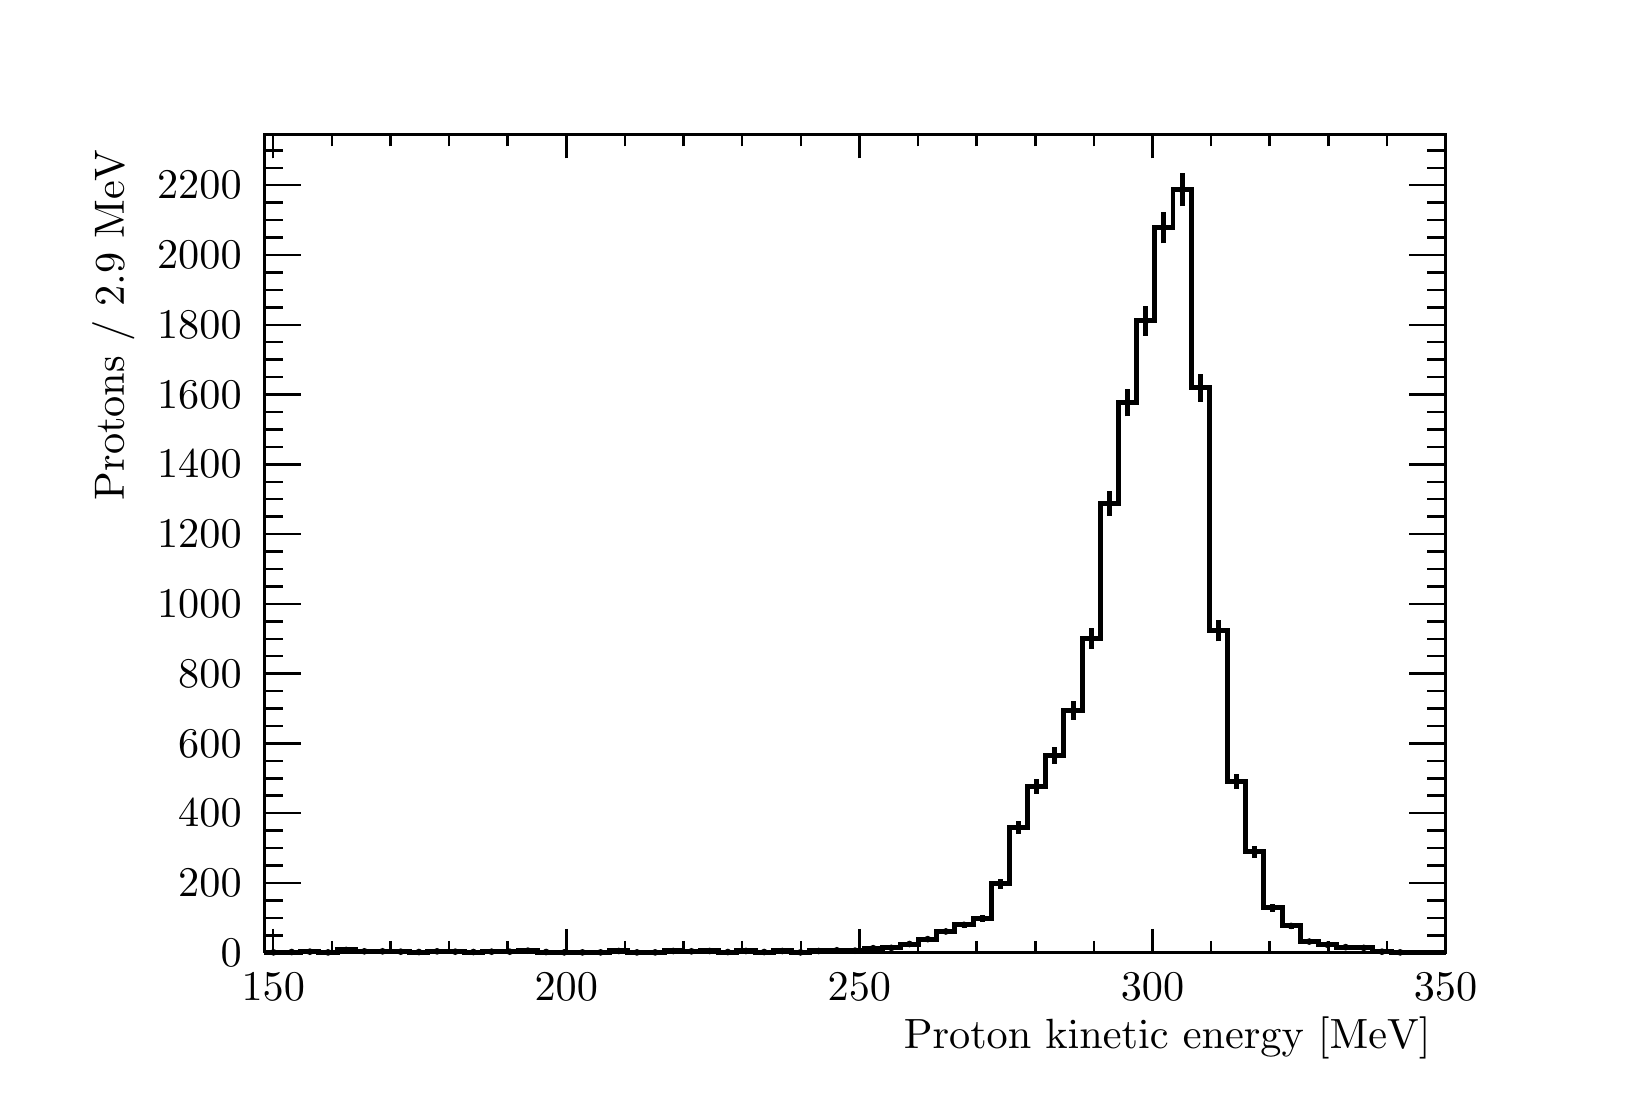
\begin{tikzpicture}
\pgfdeclareplotmark{cross} {
\pgfpathmoveto{\pgfpoint{-0.3\pgfplotmarksize}{\pgfplotmarksize}}
\pgfpathlineto{\pgfpoint{+0.3\pgfplotmarksize}{\pgfplotmarksize}}
\pgfpathlineto{\pgfpoint{+0.3\pgfplotmarksize}{0.3\pgfplotmarksize}}
\pgfpathlineto{\pgfpoint{+1\pgfplotmarksize}{0.3\pgfplotmarksize}}
\pgfpathlineto{\pgfpoint{+1\pgfplotmarksize}{-0.3\pgfplotmarksize}}
\pgfpathlineto{\pgfpoint{+0.3\pgfplotmarksize}{-0.3\pgfplotmarksize}}
\pgfpathlineto{\pgfpoint{+0.3\pgfplotmarksize}{-1.\pgfplotmarksize}}
\pgfpathlineto{\pgfpoint{-0.3\pgfplotmarksize}{-1.\pgfplotmarksize}}
\pgfpathlineto{\pgfpoint{-0.3\pgfplotmarksize}{-0.3\pgfplotmarksize}}
\pgfpathlineto{\pgfpoint{-1.\pgfplotmarksize}{-0.3\pgfplotmarksize}}
\pgfpathlineto{\pgfpoint{-1.\pgfplotmarksize}{0.3\pgfplotmarksize}}
\pgfpathlineto{\pgfpoint{-0.3\pgfplotmarksize}{0.3\pgfplotmarksize}}
\pgfpathclose
\pgfusepathqstroke
}
\pgfdeclareplotmark{cross*} {
\pgfpathmoveto{\pgfpoint{-0.3\pgfplotmarksize}{\pgfplotmarksize}}
\pgfpathlineto{\pgfpoint{+0.3\pgfplotmarksize}{\pgfplotmarksize}}
\pgfpathlineto{\pgfpoint{+0.3\pgfplotmarksize}{0.3\pgfplotmarksize}}
\pgfpathlineto{\pgfpoint{+1\pgfplotmarksize}{0.3\pgfplotmarksize}}
\pgfpathlineto{\pgfpoint{+1\pgfplotmarksize}{-0.3\pgfplotmarksize}}
\pgfpathlineto{\pgfpoint{+0.3\pgfplotmarksize}{-0.3\pgfplotmarksize}}
\pgfpathlineto{\pgfpoint{+0.3\pgfplotmarksize}{-1.\pgfplotmarksize}}
\pgfpathlineto{\pgfpoint{-0.3\pgfplotmarksize}{-1.\pgfplotmarksize}}
\pgfpathlineto{\pgfpoint{-0.3\pgfplotmarksize}{-0.3\pgfplotmarksize}}
\pgfpathlineto{\pgfpoint{-1.\pgfplotmarksize}{-0.3\pgfplotmarksize}}
\pgfpathlineto{\pgfpoint{-1.\pgfplotmarksize}{0.3\pgfplotmarksize}}
\pgfpathlineto{\pgfpoint{-0.3\pgfplotmarksize}{0.3\pgfplotmarksize}}
\pgfpathclose
\pgfusepathqfillstroke
}
\pgfdeclareplotmark{newstar} {
\pgfpathmoveto{\pgfqpoint{0pt}{\pgfplotmarksize}}
\pgfpathlineto{\pgfqpointpolar{44}{0.5\pgfplotmarksize}}
\pgfpathlineto{\pgfqpointpolar{18}{\pgfplotmarksize}}
\pgfpathlineto{\pgfqpointpolar{-20}{0.5\pgfplotmarksize}}
\pgfpathlineto{\pgfqpointpolar{-54}{\pgfplotmarksize}}
\pgfpathlineto{\pgfqpointpolar{-90}{0.5\pgfplotmarksize}}
\pgfpathlineto{\pgfqpointpolar{234}{\pgfplotmarksize}}
\pgfpathlineto{\pgfqpointpolar{198}{0.5\pgfplotmarksize}}
\pgfpathlineto{\pgfqpointpolar{162}{\pgfplotmarksize}}
\pgfpathlineto{\pgfqpointpolar{134}{0.5\pgfplotmarksize}}
\pgfpathclose
\pgfusepathqstroke
}
\pgfdeclareplotmark{newstar*} {
\pgfpathmoveto{\pgfqpoint{0pt}{\pgfplotmarksize}}
\pgfpathlineto{\pgfqpointpolar{44}{0.5\pgfplotmarksize}}
\pgfpathlineto{\pgfqpointpolar{18}{\pgfplotmarksize}}
\pgfpathlineto{\pgfqpointpolar{-20}{0.5\pgfplotmarksize}}
\pgfpathlineto{\pgfqpointpolar{-54}{\pgfplotmarksize}}
\pgfpathlineto{\pgfqpointpolar{-90}{0.5\pgfplotmarksize}}
\pgfpathlineto{\pgfqpointpolar{234}{\pgfplotmarksize}}
\pgfpathlineto{\pgfqpointpolar{198}{0.5\pgfplotmarksize}}
\pgfpathlineto{\pgfqpointpolar{162}{\pgfplotmarksize}}
\pgfpathlineto{\pgfqpointpolar{134}{0.5\pgfplotmarksize}}
\pgfpathclose
\pgfusepathqfillstroke
}
\definecolor{c}{rgb}{1,1,1};
\draw [color=c, fill=c] (0,0) rectangle (20,13.4957);
\draw [color=c, fill=c] (3,1.75444) rectangle (18,12.1461);
\definecolor{c}{rgb}{0,0,0};
\draw [c,line width=0.9] (3,1.75444) -- (3,12.1461) -- (18,12.1461) -- (18,1.75444) -- (3,1.75444);
\definecolor{c}{rgb}{1,1,1};
\draw [color=c, fill=c] (3,1.75444) rectangle (18,12.1461);
\definecolor{c}{rgb}{0,0,0};
\draw [c,line width=0.9] (3,1.75444) -- (3,12.1461) -- (18,12.1461) -- (18,1.75444) -- (3,1.75444);
\draw [c,line width=1.8] (3.11538,1.75444) -- (3.11538,1.75887);
\draw [c,line width=1.8] (3.11538,1.75887) -- (3.11538,1.7633);
\foreach \P in {(3.11538,1.75887)}{\draw[mark options={color=c,fill=c},mark size=2.402402pt,mark=*,mark size=1pt] plot coordinates {\P};}
\draw [c,line width=1.8] (3.34615,1.75704) -- (3.34615,1.7633);
\draw [c,line width=1.8] (3.34615,1.7633) -- (3.34615,1.76957);
\foreach \P in {(3.34615,1.7633)}{\draw[mark options={color=c,fill=c},mark size=2.402402pt,mark=*,mark size=1pt] plot coordinates {\P};}
\draw [c,line width=1.8] (3.57692,1.76006) -- (3.57692,1.76773);
\draw [c,line width=1.8] (3.57692,1.76773) -- (3.57692,1.77541);
\foreach \P in {(3.57692,1.76773)}{\draw[mark options={color=c,fill=c},mark size=2.402402pt,mark=*,mark size=1pt] plot coordinates {\P};}
\draw [c,line width=1.8] (3.80769,1.75444) -- (3.80769,1.75887);
\draw [c,line width=1.8] (3.80769,1.75887) -- (3.80769,1.7633);
\foreach \P in {(3.80769,1.75887)}{\draw[mark options={color=c,fill=c},mark size=2.402402pt,mark=*,mark size=1pt] plot coordinates {\P};}
\draw [c,line width=1.8] (4.03846,1.77735) -- (4.03846,1.78989);
\draw [c,line width=1.8] (4.03846,1.78989) -- (4.03846,1.80242);
\foreach \P in {(4.03846,1.78989)}{\draw[mark options={color=c,fill=c},mark size=2.402402pt,mark=*,mark size=1pt] plot coordinates {\P};}
\draw [c,line width=1.8] (4.26923,1.7633) -- (4.26923,1.77216);
\draw [c,line width=1.8] (4.26923,1.77216) -- (4.26923,1.78102);
\foreach \P in {(4.26923,1.77216)}{\draw[mark options={color=c,fill=c},mark size=2.402402pt,mark=*,mark size=1pt] plot coordinates {\P};}
\draw [c,line width=1.8] (4.5,1.7633) -- (4.5,1.77216);
\draw [c,line width=1.8] (4.5,1.77216) -- (4.5,1.78102);
\foreach \P in {(4.5,1.77216)}{\draw[mark options={color=c,fill=c},mark size=2.402402pt,mark=*,mark size=1pt] plot coordinates {\P};}
\draw [c,line width=1.8] (4.73077,1.76006) -- (4.73077,1.76773);
\draw [c,line width=1.8] (4.73077,1.76773) -- (4.73077,1.77541);
\foreach \P in {(4.73077,1.76773)}{\draw[mark options={color=c,fill=c},mark size=2.402402pt,mark=*,mark size=1pt] plot coordinates {\P};}
\draw [c,line width=1.8] (4.96154,1.75704) -- (4.96154,1.7633);
\draw [c,line width=1.8] (4.96154,1.7633) -- (4.96154,1.76957);
\foreach \P in {(4.96154,1.7633)}{\draw[mark options={color=c,fill=c},mark size=2.402402pt,mark=*,mark size=1pt] plot coordinates {\P};}
\draw [c,line width=1.8] (5.19231,1.7633) -- (5.19231,1.77216);
\draw [c,line width=1.8] (5.19231,1.77216) -- (5.19231,1.78102);
\foreach \P in {(5.19231,1.77216)}{\draw[mark options={color=c,fill=c},mark size=2.402402pt,mark=*,mark size=1pt] plot coordinates {\P};}
\draw [c,line width=1.8] (5.42308,1.76006) -- (5.42308,1.76773);
\draw [c,line width=1.8] (5.42308,1.76773) -- (5.42308,1.77541);
\foreach \P in {(5.42308,1.76773)}{\draw[mark options={color=c,fill=c},mark size=2.402402pt,mark=*,mark size=1pt] plot coordinates {\P};}
\draw [c,line width=1.8] (5.65385,1.75704) -- (5.65385,1.7633);
\draw [c,line width=1.8] (5.65385,1.7633) -- (5.65385,1.76957);
\foreach \P in {(5.65385,1.7633)}{\draw[mark options={color=c,fill=c},mark size=2.402402pt,mark=*,mark size=1pt] plot coordinates {\P};}
\draw [c,line width=1.8] (5.88462,1.76006) -- (5.88462,1.76773);
\draw [c,line width=1.8] (5.88462,1.76773) -- (5.88462,1.77541);
\foreach \P in {(5.88462,1.76773)}{\draw[mark options={color=c,fill=c},mark size=2.402402pt,mark=*,mark size=1pt] plot coordinates {\P};}
\draw [c,line width=1.8] (6.11538,1.76006) -- (6.11538,1.76773);
\draw [c,line width=1.8] (6.11538,1.76773) -- (6.11538,1.77541);
\foreach \P in {(6.11538,1.76773)}{\draw[mark options={color=c,fill=c},mark size=2.402402pt,mark=*,mark size=1pt] plot coordinates {\P};}
\draw [c,line width=1.8] (6.34615,1.77017) -- (6.34615,1.78102);
\draw [c,line width=1.8] (6.34615,1.78102) -- (6.34615,1.79188);
\foreach \P in {(6.34615,1.78102)}{\draw[mark options={color=c,fill=c},mark size=2.402402pt,mark=*,mark size=1pt] plot coordinates {\P};}
\draw [c,line width=1.8] (6.57692,1.75704) -- (6.57692,1.7633);
\draw [c,line width=1.8] (6.57692,1.7633) -- (6.57692,1.76957);
\foreach \P in {(6.57692,1.7633)}{\draw[mark options={color=c,fill=c},mark size=2.402402pt,mark=*,mark size=1pt] plot coordinates {\P};}
\draw [c,line width=1.8] (6.80769,1.75444) -- (6.80769,1.75887);
\draw [c,line width=1.8] (6.80769,1.75887) -- (6.80769,1.7633);
\foreach \P in {(6.80769,1.75887)}{\draw[mark options={color=c,fill=c},mark size=2.402402pt,mark=*,mark size=1pt] plot coordinates {\P};}
\draw [c,line width=1.8] (7.03846,1.75444) -- (7.03846,1.75887);
\draw [c,line width=1.8] (7.03846,1.75887) -- (7.03846,1.7633);
\foreach \P in {(7.03846,1.75887)}{\draw[mark options={color=c,fill=c},mark size=2.402402pt,mark=*,mark size=1pt] plot coordinates {\P};}
\draw [c,line width=1.8] (7.26923,1.75444) -- (7.26923,1.75887);
\draw [c,line width=1.8] (7.26923,1.75887) -- (7.26923,1.7633);
\foreach \P in {(7.26923,1.75887)}{\draw[mark options={color=c,fill=c},mark size=2.402402pt,mark=*,mark size=1pt] plot coordinates {\P};}
\draw [c,line width=1.8] (7.5,1.76669) -- (7.5,1.77659);
\draw [c,line width=1.8] (7.5,1.77659) -- (7.5,1.7865);
\foreach \P in {(7.5,1.77659)}{\draw[mark options={color=c,fill=c},mark size=2.402402pt,mark=*,mark size=1pt] plot coordinates {\P};}
\draw [c,line width=1.8] (7.73077,1.75444) -- (7.73077,1.75887);
\draw [c,line width=1.8] (7.73077,1.75887) -- (7.73077,1.7633);
\foreach \P in {(7.73077,1.75887)}{\draw[mark options={color=c,fill=c},mark size=2.402402pt,mark=*,mark size=1pt] plot coordinates {\P};}
\draw [c,line width=1.8] (7.96154,1.75444) -- (7.96154,1.75887);
\draw [c,line width=1.8] (7.96154,1.75887) -- (7.96154,1.7633);
\foreach \P in {(7.96154,1.75887)}{\draw[mark options={color=c,fill=c},mark size=2.402402pt,mark=*,mark size=1pt] plot coordinates {\P};}
\draw [c,line width=1.8] (8.19231,1.76669) -- (8.19231,1.77659);
\draw [c,line width=1.8] (8.19231,1.77659) -- (8.19231,1.7865);
\foreach \P in {(8.19231,1.77659)}{\draw[mark options={color=c,fill=c},mark size=2.402402pt,mark=*,mark size=1pt] plot coordinates {\P};}
\draw [c,line width=1.8] (8.42308,1.7633) -- (8.42308,1.77216);
\draw [c,line width=1.8] (8.42308,1.77216) -- (8.42308,1.78102);
\foreach \P in {(8.42308,1.77216)}{\draw[mark options={color=c,fill=c},mark size=2.402402pt,mark=*,mark size=1pt] plot coordinates {\P};}
\draw [c,line width=1.8] (8.65385,1.76669) -- (8.65385,1.77659);
\draw [c,line width=1.8] (8.65385,1.77659) -- (8.65385,1.7865);
\foreach \P in {(8.65385,1.77659)}{\draw[mark options={color=c,fill=c},mark size=2.402402pt,mark=*,mark size=1pt] plot coordinates {\P};}
\draw [c,line width=1.8] (8.88462,1.75704) -- (8.88462,1.7633);
\draw [c,line width=1.8] (8.88462,1.7633) -- (8.88462,1.76957);
\foreach \P in {(8.88462,1.7633)}{\draw[mark options={color=c,fill=c},mark size=2.402402pt,mark=*,mark size=1pt] plot coordinates {\P};}
\draw [c,line width=1.8] (9.11539,1.76669) -- (9.11539,1.77659);
\draw [c,line width=1.8] (9.11539,1.77659) -- (9.11539,1.7865);
\foreach \P in {(9.11539,1.77659)}{\draw[mark options={color=c,fill=c},mark size=2.402402pt,mark=*,mark size=1pt] plot coordinates {\P};}
\draw [c,line width=1.8] (9.34615,1.75704) -- (9.34615,1.7633);
\draw [c,line width=1.8] (9.34615,1.7633) -- (9.34615,1.76957);
\foreach \P in {(9.34615,1.7633)}{\draw[mark options={color=c,fill=c},mark size=2.402402pt,mark=*,mark size=1pt] plot coordinates {\P};}
\draw [c,line width=1.8] (9.57692,1.76669) -- (9.57692,1.77659);
\draw [c,line width=1.8] (9.57692,1.77659) -- (9.57692,1.7865);
\foreach \P in {(9.57692,1.77659)}{\draw[mark options={color=c,fill=c},mark size=2.402402pt,mark=*,mark size=1pt] plot coordinates {\P};}
\draw [c,line width=1.8] (9.80769,1.75444) -- (9.80769,1.75887);
\draw [c,line width=1.8] (9.80769,1.75887) -- (9.80769,1.7633);
\foreach \P in {(9.80769,1.75887)}{\draw[mark options={color=c,fill=c},mark size=2.402402pt,mark=*,mark size=1pt] plot coordinates {\P};}
\draw [c,line width=1.8] (10.0385,1.76669) -- (10.0385,1.77659);
\draw [c,line width=1.8] (10.0385,1.77659) -- (10.0385,1.7865);
\foreach \P in {(10.0385,1.77659)}{\draw[mark options={color=c,fill=c},mark size=2.402402pt,mark=*,mark size=1pt] plot coordinates {\P};}
\draw [c,line width=1.8] (10.2692,1.77373) -- (10.2692,1.78546);
\draw [c,line width=1.8] (10.2692,1.78546) -- (10.2692,1.79718);
\foreach \P in {(10.2692,1.78546)}{\draw[mark options={color=c,fill=c},mark size=2.402402pt,mark=*,mark size=1pt] plot coordinates {\P};}
\draw [c,line width=1.8] (10.5,1.77017) -- (10.5,1.78102);
\draw [c,line width=1.8] (10.5,1.78102) -- (10.5,1.79188);
\foreach \P in {(10.5,1.78102)}{\draw[mark options={color=c,fill=c},mark size=2.402402pt,mark=*,mark size=1pt] plot coordinates {\P};}
\draw [c,line width=1.8] (10.7308,1.79606) -- (10.7308,1.81204);
\draw [c,line width=1.8] (10.7308,1.81204) -- (10.7308,1.82801);
\foreach \P in {(10.7308,1.81204)}{\draw[mark options={color=c,fill=c},mark size=2.402402pt,mark=*,mark size=1pt] plot coordinates {\P};}
\draw [c,line width=1.8] (10.9615,1.79989) -- (10.9615,1.81647);
\draw [c,line width=1.8] (10.9615,1.81647) -- (10.9615,1.83305);
\foreach \P in {(10.9615,1.81647)}{\draw[mark options={color=c,fill=c},mark size=2.402402pt,mark=*,mark size=1pt] plot coordinates {\P};}
\draw [c,line width=1.8] (11.1923,1.84305) -- (11.1923,1.86521);
\draw [c,line width=1.8] (11.1923,1.86521) -- (11.1923,1.88736);
\foreach \P in {(11.1923,1.86521)}{\draw[mark options={color=c,fill=c},mark size=2.402402pt,mark=*,mark size=1pt] plot coordinates {\P};}
\draw [c,line width=1.8] (11.4231,1.89956) -- (11.4231,1.92723);
\draw [c,line width=1.8] (11.4231,1.92723) -- (11.4231,1.9549);
\foreach \P in {(11.4231,1.92723)}{\draw[mark options={color=c,fill=c},mark size=2.402402pt,mark=*,mark size=1pt] plot coordinates {\P};}
\draw [c,line width=1.8] (11.6538,1.9901) -- (11.6538,2.02471);
\draw [c,line width=1.8] (11.6538,2.02471) -- (11.6538,2.05931);
\foreach \P in {(11.6538,2.02471)}{\draw[mark options={color=c,fill=c},mark size=2.402402pt,mark=*,mark size=1pt] plot coordinates {\P};}
\draw [c,line width=1.8] (11.8846,2.06926) -- (11.8846,2.10889);
\draw [c,line width=1.8] (11.8846,2.10889) -- (11.8846,2.14851);
\foreach \P in {(11.8846,2.10889)}{\draw[mark options={color=c,fill=c},mark size=2.402402pt,mark=*,mark size=1pt] plot coordinates {\P};}
\draw [c,line width=1.8] (12.1154,2.14478) -- (12.1154,2.18864);
\draw [c,line width=1.8] (12.1154,2.18864) -- (12.1154,2.2325);
\foreach \P in {(12.1154,2.18864)}{\draw[mark options={color=c,fill=c},mark size=2.402402pt,mark=*,mark size=1pt] plot coordinates {\P};}
\draw [c,line width=1.8] (12.3462,2.56935) -- (12.3462,2.63169);
\draw [c,line width=1.8] (12.3462,2.63169) -- (12.3462,2.69404);
\foreach \P in {(12.3462,2.63169)}{\draw[mark options={color=c,fill=c},mark size=2.402402pt,mark=*,mark size=1pt] plot coordinates {\P};}
\draw [c,line width=1.8] (12.5769,3.26538) -- (12.5769,3.34945);
\draw [c,line width=1.8] (12.5769,3.34945) -- (12.5769,3.43351);
\foreach \P in {(12.5769,3.34945)}{\draw[mark options={color=c,fill=c},mark size=2.402402pt,mark=*,mark size=1pt] plot coordinates {\P};}
\draw [c,line width=1.8] (12.8077,3.77106) -- (12.8077,3.86782);
\draw [c,line width=1.8] (12.8077,3.86782) -- (12.8077,3.96459);
\foreach \P in {(12.8077,3.86782)}{\draw[mark options={color=c,fill=c},mark size=2.402402pt,mark=*,mark size=1pt] plot coordinates {\P};}
\draw [c,line width=1.8] (13.0385,4.1524) -- (13.0385,4.25771);
\draw [c,line width=1.8] (13.0385,4.25771) -- (13.0385,4.36303);
\foreach \P in {(13.0385,4.25771)}{\draw[mark options={color=c,fill=c},mark size=2.402402pt,mark=*,mark size=1pt] plot coordinates {\P};}
\draw [c,line width=1.8] (13.2692,4.71254) -- (13.2692,4.82926);
\draw [c,line width=1.8] (13.2692,4.82926) -- (13.2692,4.94597);
\foreach \P in {(13.2692,4.82926)}{\draw[mark options={color=c,fill=c},mark size=2.402402pt,mark=*,mark size=1pt] plot coordinates {\P};}
\draw [c,line width=1.8] (13.5,5.60904) -- (13.5,5.74195);
\draw [c,line width=1.8] (13.5,5.74195) -- (13.5,5.87487);
\foreach \P in {(13.5,5.74195)}{\draw[mark options={color=c,fill=c},mark size=2.402402pt,mark=*,mark size=1pt] plot coordinates {\P};}
\draw [c,line width=1.8] (13.7308,7.302) -- (13.7308,7.46101);
\draw [c,line width=1.8] (13.7308,7.46101) -- (13.7308,7.62002);
\foreach \P in {(13.7308,7.46101)}{\draw[mark options={color=c,fill=c},mark size=2.402402pt,mark=*,mark size=1pt] plot coordinates {\P};}
\draw [c,line width=1.8] (13.9615,8.5655) -- (13.9615,8.74145);
\draw [c,line width=1.8] (13.9615,8.74145) -- (13.9615,8.91739);
\foreach \P in {(13.9615,8.74145)}{\draw[mark options={color=c,fill=c},mark size=2.402402pt,mark=*,mark size=1pt] plot coordinates {\P};}
\draw [c,line width=1.8] (14.1923,9.58965) -- (14.1923,9.7782);
\draw [c,line width=1.8] (14.1923,9.7782) -- (14.1923,9.96675);
\foreach \P in {(14.1923,9.7782)}{\draw[mark options={color=c,fill=c},mark size=2.402402pt,mark=*,mark size=1pt] plot coordinates {\P};}
\draw [c,line width=1.8] (14.4231,10.7636) -- (14.4231,10.9656);
\draw [c,line width=1.8] (14.4231,10.9656) -- (14.4231,11.1676);
\foreach \P in {(14.4231,10.9656)}{\draw[mark options={color=c,fill=c},mark size=2.402402pt,mark=*,mark size=1pt] plot coordinates {\P};}
\draw [c,line width=1.8] (14.6538,11.2369) -- (14.6538,11.4441);
\draw [c,line width=1.8] (14.6538,11.4441) -- (14.6538,11.6513);
\foreach \P in {(14.6538,11.4441)}{\draw[mark options={color=c,fill=c},mark size=2.402402pt,mark=*,mark size=1pt] plot coordinates {\P};}
\draw [c,line width=1.8] (14.8846,8.75363) -- (14.8846,8.93196);
\draw [c,line width=1.8] (14.8846,8.93196) -- (14.8846,9.11029);
\foreach \P in {(14.8846,8.93196)}{\draw[mark options={color=c,fill=c},mark size=2.402402pt,mark=*,mark size=1pt] plot coordinates {\P};}
\draw [c,line width=1.8] (15.1154,5.70925) -- (15.1154,5.84385);
\draw [c,line width=1.8] (15.1154,5.84385) -- (15.1154,5.97846);
\foreach \P in {(15.1154,5.84385)}{\draw[mark options={color=c,fill=c},mark size=2.402402pt,mark=*,mark size=1pt] plot coordinates {\P};}
\draw [c,line width=1.8] (15.3462,3.83168) -- (15.3462,3.92985);
\draw [c,line width=1.8] (15.3462,3.92985) -- (15.3462,4.02802);
\foreach \P in {(15.3462,3.92985)}{\draw[mark options={color=c,fill=c},mark size=2.402402pt,mark=*,mark size=1pt] plot coordinates {\P};}
\draw [c,line width=1.8] (15.5769,2.95956) -- (15.5769,3.03488);
\draw [c,line width=1.8] (15.5769,3.03488) -- (15.5769,3.11019);
\foreach \P in {(15.5769,3.03488)}{\draw[mark options={color=c,fill=c},mark size=2.402402pt,mark=*,mark size=1pt] plot coordinates {\P};}
\draw [c,line width=1.8] (15.8077,2.27566) -- (15.8077,2.32598);
\draw [c,line width=1.8] (15.8077,2.32598) -- (15.8077,2.37631);
\foreach \P in {(15.8077,2.32598)}{\draw[mark options={color=c,fill=c},mark size=2.402402pt,mark=*,mark size=1pt] plot coordinates {\P};}
\draw [c,line width=1.8] (16.0385,2.05672) -- (16.0385,2.09559);
\draw [c,line width=1.8] (16.0385,2.09559) -- (16.0385,2.13447);
\foreach \P in {(16.0385,2.09559)}{\draw[mark options={color=c,fill=c},mark size=2.402402pt,mark=*,mark size=1pt] plot coordinates {\P};}
\draw [c,line width=1.8] (16.2692,1.87116) -- (16.2692,1.89622);
\draw [c,line width=1.8] (16.2692,1.89622) -- (16.2692,1.92128);
\foreach \P in {(16.2692,1.89622)}{\draw[mark options={color=c,fill=c},mark size=2.402402pt,mark=*,mark size=1pt] plot coordinates {\P};}
\draw [c,line width=1.8] (16.5,1.8351) -- (16.5,1.85634);
\draw [c,line width=1.8] (16.5,1.85634) -- (16.5,1.87759);
\foreach \P in {(16.5,1.85634)}{\draw[mark options={color=c,fill=c},mark size=2.402402pt,mark=*,mark size=1pt] plot coordinates {\P};}
\draw [c,line width=1.8] (16.7308,1.80761) -- (16.7308,1.82533);
\draw [c,line width=1.8] (16.7308,1.82533) -- (16.7308,1.84305);
\foreach \P in {(16.7308,1.82533)}{\draw[mark options={color=c,fill=c},mark size=2.402402pt,mark=*,mark size=1pt] plot coordinates {\P};}
\draw [c,line width=1.8] (16.9615,1.79989) -- (16.9615,1.81647);
\draw [c,line width=1.8] (16.9615,1.81647) -- (16.9615,1.83305);
\foreach \P in {(16.9615,1.81647)}{\draw[mark options={color=c,fill=c},mark size=2.402402pt,mark=*,mark size=1pt] plot coordinates {\P};}
\draw [c,line width=1.8] (17.1923,1.76006) -- (17.1923,1.76773);
\draw [c,line width=1.8] (17.1923,1.76773) -- (17.1923,1.77541);
\foreach \P in {(17.1923,1.76773)}{\draw[mark options={color=c,fill=c},mark size=2.402402pt,mark=*,mark size=1pt] plot coordinates {\P};}
\draw [c,line width=1.8] (17.4231,1.75444) -- (17.4231,1.75887);
\draw [c,line width=1.8] (17.4231,1.75887) -- (17.4231,1.7633);
\foreach \P in {(17.4231,1.75887)}{\draw[mark options={color=c,fill=c},mark size=2.402402pt,mark=*,mark size=1pt] plot coordinates {\P};}
\draw [c,line width=1.8] (3,1.75887) -- (3.23077,1.75887) -- (3.23077,1.7633) -- (3.46154,1.7633) -- (3.46154,1.76773) -- (3.69231,1.76773) -- (3.69231,1.75887) -- (3.92308,1.75887) -- (3.92308,1.78989) -- (4.15385,1.78989) -- (4.15385,1.77216) --
 (4.38462,1.77216) -- (4.38462,1.77216) -- (4.61538,1.77216) -- (4.61538,1.76773) -- (4.84615,1.76773) -- (4.84615,1.7633) -- (5.07692,1.7633) -- (5.07692,1.77216) -- (5.30769,1.77216) -- (5.30769,1.76773) -- (5.53846,1.76773) -- (5.53846,1.7633) --
 (5.76923,1.7633) -- (5.76923,1.76773) -- (6,1.76773) -- (6,1.76773) -- (6.23077,1.76773) -- (6.23077,1.78102) -- (6.46154,1.78102) -- (6.46154,1.7633) -- (6.69231,1.7633) -- (6.69231,1.75887) -- (6.92308,1.75887) -- (6.92308,1.75887) --
 (7.15385,1.75887) -- (7.15385,1.75887) -- (7.38462,1.75887) -- (7.38462,1.77659) -- (7.61538,1.77659) -- (7.61538,1.75887) -- (7.84615,1.75887) -- (7.84615,1.75887) -- (8.07692,1.75887) -- (8.07692,1.77659) -- (8.30769,1.77659) -- (8.30769,1.77216)
 -- (8.53846,1.77216) -- (8.53846,1.77659) -- (8.76923,1.77659) -- (8.76923,1.7633) -- (9,1.7633) -- (9,1.77659) -- (9.23077,1.77659) -- (9.23077,1.7633) -- (9.46154,1.7633) -- (9.46154,1.77659) -- (9.69231,1.77659) -- (9.69231,1.75887) --
 (9.92308,1.75887) -- (9.92308,1.77659) -- (10.1538,1.77659) -- (10.1538,1.78546) -- (10.3846,1.78546) -- (10.3846,1.78102) -- (10.6154,1.78102) -- (10.6154,1.81204) -- (10.8462,1.81204) -- (10.8462,1.81647) -- (11.0769,1.81647) -- (11.0769,1.86521)
 -- (11.3077,1.86521) -- (11.3077,1.92723) -- (11.5385,1.92723) -- (11.5385,2.02471) -- (11.7692,2.02471) -- (11.7692,2.10889) -- (12,2.10889) -- (12,2.18864) -- (12.2308,2.18864) -- (12.2308,2.63169) -- (12.4615,2.63169) -- (12.4615,3.34945) --
 (12.6923,3.34945) -- (12.6923,3.86782) -- (12.9231,3.86782) -- (12.9231,4.25771) -- (13.1538,4.25771) -- (13.1538,4.82926) -- (13.3846,4.82926) -- (13.3846,5.74195) -- (13.6154,5.74195) -- (13.6154,7.46101) -- (13.8462,7.46101) -- (13.8462,8.74145)
 -- (14.0769,8.74145) -- (14.0769,9.7782) -- (14.3077,9.7782) -- (14.3077,10.9656) -- (14.5385,10.9656) -- (14.5385,11.4441) -- (14.7692,11.4441) -- (14.7692,8.93196) -- (15,8.93196) -- (15,5.84385) -- (15.2308,5.84385) -- (15.2308,3.92985) --
 (15.4615,3.92985) -- (15.4615,3.03488) -- (15.6923,3.03488) -- (15.6923,2.32598) -- (15.9231,2.32598) -- (15.9231,2.09559) -- (16.1538,2.09559) -- (16.1538,1.89622) -- (16.3846,1.89622) -- (16.3846,1.85634) -- (16.6154,1.85634) -- (16.6154,1.82533)
 -- (16.8462,1.82533) -- (16.8462,1.81647) -- (17.0769,1.81647) -- (17.0769,1.76773) -- (17.3077,1.76773) -- (17.3077,1.75887) -- (17.5385,1.75887) -- (17.5385,1.75444) -- (17.7692,1.75444) -- (17.7692,1.75444) -- (18,1.75444);
\draw [c,line width=0.9] (3,1.75444) -- (18,1.75444);
\draw [c,line width=0.9] (3.11166,2.05809) -- (3.11166,1.75444);
\draw [c,line width=0.9] (3.85608,1.90627) -- (3.85608,1.75444);
\draw [c,line width=0.9] (4.6005,1.90627) -- (4.6005,1.75444);
\draw [c,line width=0.9] (5.34491,1.90627) -- (5.34491,1.75444);
\draw [c,line width=0.9] (6.08933,1.90627) -- (6.08933,1.75444);
\draw [c,line width=0.9] (6.83375,2.05809) -- (6.83375,1.75444);
\draw [c,line width=0.9] (7.57816,1.90627) -- (7.57816,1.75444);
\draw [c,line width=0.9] (8.32258,1.90627) -- (8.32258,1.75444);
\draw [c,line width=0.9] (9.067,1.90627) -- (9.067,1.75444);
\draw [c,line width=0.9] (9.81141,1.90627) -- (9.81141,1.75444);
\draw [c,line width=0.9] (10.5558,2.05809) -- (10.5558,1.75444);
\draw [c,line width=0.9] (11.3002,1.90627) -- (11.3002,1.75444);
\draw [c,line width=0.9] (12.0447,1.90627) -- (12.0447,1.75444);
\draw [c,line width=0.9] (12.7891,1.90627) -- (12.7891,1.75444);
\draw [c,line width=0.9] (13.5335,1.90627) -- (13.5335,1.75444);
\draw [c,line width=0.9] (14.2779,2.05809) -- (14.2779,1.75444);
\draw [c,line width=0.9] (15.0223,1.90627) -- (15.0223,1.75444);
\draw [c,line width=0.9] (15.7667,1.90627) -- (15.7667,1.75444);
\draw [c,line width=0.9] (16.5112,1.90627) -- (16.5112,1.75444);
\draw [c,line width=0.9] (17.2556,1.90627) -- (17.2556,1.75444);
\draw [c,line width=0.9] (18,2.05809) -- (18,1.75444);
\draw [c,line width=0.9] (3.11166,2.05809) -- (3.11166,1.75444);
\draw [c,line width=0.9] (18,2.05809) -- (18,1.75444);
\draw [anchor=base] (3.11166,1.14713) node[scale=1.52731, color=c, rotate=0]{150};
\draw [anchor=base] (6.83375,1.14713) node[scale=1.52731, color=c, rotate=0]{200};
\draw [anchor=base] (10.5558,1.14713) node[scale=1.52731, color=c, rotate=0]{250};
\draw [anchor=base] (14.2779,1.14713) node[scale=1.52731, color=c, rotate=0]{300};
\draw [anchor=base] (18,1.14713) node[scale=1.52731, color=c, rotate=0]{350};
\draw [anchor= east] (18,0.674785) node[scale=1.52731, color=c, rotate=0]{ Proton kinetic energy [MeV]};
\draw [c,line width=0.9] (3,12.1461) -- (18,12.1461);
\draw [c,line width=0.9] (3.11166,11.8425) -- (3.11166,12.1461);
\draw [c,line width=0.9] (3.85608,11.9943) -- (3.85608,12.1461);
\draw [c,line width=0.9] (4.6005,11.9943) -- (4.6005,12.1461);
\draw [c,line width=0.9] (5.34491,11.9943) -- (5.34491,12.1461);
\draw [c,line width=0.9] (6.08933,11.9943) -- (6.08933,12.1461);
\draw [c,line width=0.9] (6.83375,11.8425) -- (6.83375,12.1461);
\draw [c,line width=0.9] (7.57816,11.9943) -- (7.57816,12.1461);
\draw [c,line width=0.9] (8.32258,11.9943) -- (8.32258,12.1461);
\draw [c,line width=0.9] (9.067,11.9943) -- (9.067,12.1461);
\draw [c,line width=0.9] (9.81141,11.9943) -- (9.81141,12.1461);
\draw [c,line width=0.9] (10.5558,11.8425) -- (10.5558,12.1461);
\draw [c,line width=0.9] (11.3002,11.9943) -- (11.3002,12.1461);
\draw [c,line width=0.9] (12.0447,11.9943) -- (12.0447,12.1461);
\draw [c,line width=0.9] (12.7891,11.9943) -- (12.7891,12.1461);
\draw [c,line width=0.9] (13.5335,11.9943) -- (13.5335,12.1461);
\draw [c,line width=0.9] (14.2779,11.8425) -- (14.2779,12.1461);
\draw [c,line width=0.9] (15.0223,11.9943) -- (15.0223,12.1461);
\draw [c,line width=0.9] (15.7667,11.9943) -- (15.7667,12.1461);
\draw [c,line width=0.9] (16.5112,11.9943) -- (16.5112,12.1461);
\draw [c,line width=0.9] (17.2556,11.9943) -- (17.2556,12.1461);
\draw [c,line width=0.9] (18,11.8425) -- (18,12.1461);
\draw [c,line width=0.9] (3.11166,11.8425) -- (3.11166,12.1461);
\draw [c,line width=0.9] (18,11.8425) -- (18,12.1461);
\draw [c,line width=0.9] (3,1.75444) -- (3,12.1461);
\draw [c,line width=0.9] (3.462,1.75444) -- (3,1.75444);
\draw [c,line width=0.9] (3.231,1.97597) -- (3,1.97597);
\draw [c,line width=0.9] (3.231,2.1975) -- (3,2.1975);
\draw [c,line width=0.9] (3.231,2.41903) -- (3,2.41903);
\draw [c,line width=0.9] (3.462,2.64055) -- (3,2.64055);
\draw [c,line width=0.9] (3.231,2.86208) -- (3,2.86208);
\draw [c,line width=0.9] (3.231,3.08361) -- (3,3.08361);
\draw [c,line width=0.9] (3.231,3.30514) -- (3,3.30514);
\draw [c,line width=0.9] (3.462,3.52667) -- (3,3.52667);
\draw [c,line width=0.9] (3.231,3.7482) -- (3,3.7482);
\draw [c,line width=0.9] (3.231,3.96972) -- (3,3.96972);
\draw [c,line width=0.9] (3.231,4.19125) -- (3,4.19125);
\draw [c,line width=0.9] (3.462,4.41278) -- (3,4.41278);
\draw [c,line width=0.9] (3.231,4.63431) -- (3,4.63431);
\draw [c,line width=0.9] (3.231,4.85584) -- (3,4.85584);
\draw [c,line width=0.9] (3.231,5.07737) -- (3,5.07737);
\draw [c,line width=0.9] (3.462,5.29889) -- (3,5.29889);
\draw [c,line width=0.9] (3.231,5.52042) -- (3,5.52042);
\draw [c,line width=0.9] (3.231,5.74195) -- (3,5.74195);
\draw [c,line width=0.9] (3.231,5.96348) -- (3,5.96348);
\draw [c,line width=0.9] (3.462,6.18501) -- (3,6.18501);
\draw [c,line width=0.9] (3.231,6.40654) -- (3,6.40654);
\draw [c,line width=0.9] (3.231,6.62807) -- (3,6.62807);
\draw [c,line width=0.9] (3.231,6.84959) -- (3,6.84959);
\draw [c,line width=0.9] (3.462,7.07112) -- (3,7.07112);
\draw [c,line width=0.9] (3.231,7.29265) -- (3,7.29265);
\draw [c,line width=0.9] (3.231,7.51418) -- (3,7.51418);
\draw [c,line width=0.9] (3.231,7.73571) -- (3,7.73571);
\draw [c,line width=0.9] (3.462,7.95724) -- (3,7.95724);
\draw [c,line width=0.9] (3.231,8.17876) -- (3,8.17876);
\draw [c,line width=0.9] (3.231,8.40029) -- (3,8.40029);
\draw [c,line width=0.9] (3.231,8.62182) -- (3,8.62182);
\draw [c,line width=0.9] (3.462,8.84335) -- (3,8.84335);
\draw [c,line width=0.9] (3.231,9.06488) -- (3,9.06488);
\draw [c,line width=0.9] (3.231,9.28641) -- (3,9.28641);
\draw [c,line width=0.9] (3.231,9.50793) -- (3,9.50793);
\draw [c,line width=0.9] (3.462,9.72946) -- (3,9.72946);
\draw [c,line width=0.9] (3.231,9.95099) -- (3,9.95099);
\draw [c,line width=0.9] (3.231,10.1725) -- (3,10.1725);
\draw [c,line width=0.9] (3.231,10.394) -- (3,10.394);
\draw [c,line width=0.9] (3.462,10.6156) -- (3,10.6156);
\draw [c,line width=0.9] (3.231,10.8371) -- (3,10.8371);
\draw [c,line width=0.9] (3.231,11.0586) -- (3,11.0586);
\draw [c,line width=0.9] (3.231,11.2802) -- (3,11.2802);
\draw [c,line width=0.9] (3.462,11.5017) -- (3,11.5017);
\draw [c,line width=0.9] (3.462,11.5017) -- (3,11.5017);
\draw [c,line width=0.9] (3.231,11.7232) -- (3,11.7232);
\draw [c,line width=0.9] (3.231,11.9447) -- (3,11.9447);
\draw [anchor= east] (2.9,1.75444) node[scale=1.52731, color=c, rotate=0]{0};
\draw [anchor= east] (2.9,2.64055) node[scale=1.52731, color=c, rotate=0]{200};
\draw [anchor= east] (2.9,3.52667) node[scale=1.52731, color=c, rotate=0]{400};
\draw [anchor= east] (2.9,4.41278) node[scale=1.52731, color=c, rotate=0]{600};
\draw [anchor= east] (2.9,5.29889) node[scale=1.52731, color=c, rotate=0]{800};
\draw [anchor= east] (2.9,6.18501) node[scale=1.52731, color=c, rotate=0]{1000};
\draw [anchor= east] (2.9,7.07112) node[scale=1.52731, color=c, rotate=0]{1200};
\draw [anchor= east] (2.9,7.95724) node[scale=1.52731, color=c, rotate=0]{1400};
\draw [anchor= east] (2.9,8.84335) node[scale=1.52731, color=c, rotate=0]{1600};
\draw [anchor= east] (2.9,9.72946) node[scale=1.52731, color=c, rotate=0]{1800};
\draw [anchor= east] (2.9,10.6156) node[scale=1.52731, color=c, rotate=0]{2000};
\draw [anchor= east] (2.9,11.5017) node[scale=1.52731, color=c, rotate=0]{2200};
\draw [anchor= east] (1.08,12.1461) node[scale=1.52731, color=c, rotate=90]{Protons / 2.9~MeV};
\draw [c,line width=0.9] (18,1.75444) -- (18,12.1461);
\draw [c,line width=0.9] (17.538,1.75444) -- (18,1.75444);
\draw [c,line width=0.9] (17.769,1.97597) -- (18,1.97597);
\draw [c,line width=0.9] (17.769,2.1975) -- (18,2.1975);
\draw [c,line width=0.9] (17.769,2.41903) -- (18,2.41903);
\draw [c,line width=0.9] (17.538,2.64055) -- (18,2.64055);
\draw [c,line width=0.9] (17.769,2.86208) -- (18,2.86208);
\draw [c,line width=0.9] (17.769,3.08361) -- (18,3.08361);
\draw [c,line width=0.9] (17.769,3.30514) -- (18,3.30514);
\draw [c,line width=0.9] (17.538,3.52667) -- (18,3.52667);
\draw [c,line width=0.9] (17.769,3.7482) -- (18,3.7482);
\draw [c,line width=0.9] (17.769,3.96972) -- (18,3.96972);
\draw [c,line width=0.9] (17.769,4.19125) -- (18,4.19125);
\draw [c,line width=0.9] (17.538,4.41278) -- (18,4.41278);
\draw [c,line width=0.9] (17.769,4.63431) -- (18,4.63431);
\draw [c,line width=0.9] (17.769,4.85584) -- (18,4.85584);
\draw [c,line width=0.9] (17.769,5.07737) -- (18,5.07737);
\draw [c,line width=0.9] (17.538,5.29889) -- (18,5.29889);
\draw [c,line width=0.9] (17.769,5.52042) -- (18,5.52042);
\draw [c,line width=0.9] (17.769,5.74195) -- (18,5.74195);
\draw [c,line width=0.9] (17.769,5.96348) -- (18,5.96348);
\draw [c,line width=0.9] (17.538,6.18501) -- (18,6.18501);
\draw [c,line width=0.9] (17.769,6.40654) -- (18,6.40654);
\draw [c,line width=0.9] (17.769,6.62807) -- (18,6.62807);
\draw [c,line width=0.9] (17.769,6.84959) -- (18,6.84959);
\draw [c,line width=0.9] (17.538,7.07112) -- (18,7.07112);
\draw [c,line width=0.9] (17.769,7.29265) -- (18,7.29265);
\draw [c,line width=0.9] (17.769,7.51418) -- (18,7.51418);
\draw [c,line width=0.9] (17.769,7.73571) -- (18,7.73571);
\draw [c,line width=0.9] (17.538,7.95724) -- (18,7.95724);
\draw [c,line width=0.9] (17.769,8.17876) -- (18,8.17876);
\draw [c,line width=0.9] (17.769,8.40029) -- (18,8.40029);
\draw [c,line width=0.9] (17.769,8.62182) -- (18,8.62182);
\draw [c,line width=0.9] (17.538,8.84335) -- (18,8.84335);
\draw [c,line width=0.9] (17.769,9.06488) -- (18,9.06488);
\draw [c,line width=0.9] (17.769,9.28641) -- (18,9.28641);
\draw [c,line width=0.9] (17.769,9.50793) -- (18,9.50793);
\draw [c,line width=0.9] (17.538,9.72946) -- (18,9.72946);
\draw [c,line width=0.9] (17.769,9.95099) -- (18,9.95099);
\draw [c,line width=0.9] (17.769,10.1725) -- (18,10.1725);
\draw [c,line width=0.9] (17.769,10.394) -- (18,10.394);
\draw [c,line width=0.9] (17.538,10.6156) -- (18,10.6156);
\draw [c,line width=0.9] (17.769,10.8371) -- (18,10.8371);
\draw [c,line width=0.9] (17.769,11.0586) -- (18,11.0586);
\draw [c,line width=0.9] (17.769,11.2802) -- (18,11.2802);
\draw [c,line width=0.9] (17.538,11.5017) -- (18,11.5017);
\draw [c,line width=0.9] (17.538,11.5017) -- (18,11.5017);
\draw [c,line width=0.9] (17.769,11.7232) -- (18,11.7232);
\draw [c,line width=0.9] (17.769,11.9447) -- (18,11.9447);
\definecolor{c}{rgb}{1,1,1};
\draw [color=c, fill=c] (2,12.686) rectangle (18,13.4282);
\definecolor{c}{rgb}{0,0,0};
%\draw (10,13.0571) node[scale=1.40004, color=c, rotate=0]{Proton kinetic energy measured in $\mathit{S3}$};
\end{tikzpicture}

    \end{adjustbox}
  \end{minipage}
  \caption[Time of flight spectrum and proton kinetic energy for the unmoderated and unbent T10 beam]{Left: time of flight spectrum of the unmoderated and unbent CERN T10 beam across a baseline of \SI{10.8}{\metre}. Right: measured kinetic energies of protons in the unmoderated and unbent CERN T10 beam.}
  \label{fig:unmoderatedBeam}
\end{figure}

It is necessary to modify the T10 beam for several reasons, one of them being the lack of the low energy protons.
Additionally, it is important to reduce the multiplicity of particles entering the HPgTPC due to the speed of the optical readout which could otherwise become overwhelmed.
Finally, it is desirable to modify the proton-minimum ionising particle (MIP) ratio in order to isolate more particles which are of interest to a cross-section analysis.

Therefore, two modification are made to the beam flux in order to achieve these goals.
Firstly up to four \SI{10 x 10 x 10}{\cm} acrylic moderator blocks are placed in the beam.
These blocks have the effect of scattering the incident particles and reducing their energy.
Additionally, the HPgTPC is moved to an off-axis angle in order to maximise the ratio of protons to MIPs.
From previous GEANT~\cite{geant} simulations it is determined that the optimal off-axis angle for the HPgTPC is between \ang{2} and \ang{3}.

However, due to space constraints in the beam hall, the HPgTPC could not be moved this far off-axis.
Instead, the beam was steered approximately \ang{1} off its nominal axis to increase the angle between the beam and the HPgTPC.
A bird's-eye view diagram of the experimental setup, which shows the beam position relative to the HPgTPC, is shown in \citefig{fig:beamSetup}.

\begin{figure}[h]
  \centering
  \includegraphics[width=\linewidth]{files/figures/hptpc_beam_flux/hptpc_t10_planview}
  \caption[Bird's-eye view of the experimental setup within the T10 beam area]{Bird's-eye view of the experimental setup within the T10 beam area, from~\cite{beampaper}.}
  \label{fig:beamSetup}
\end{figure}

The effectiveness of this off-axis technique was assessed using several timing points which were used to measure the particle species and energies upstream and downstream of the HPgTPC prototype.
These timing points are shown in \citefig{fig:beamSetup} and, from upstream to downstream, consist of:
\begin{itemize}
    \item \SOne, a \SI{40 x 40 x 5}{\mm} plastic scintillator cross, described in \citesec{sec:hptpc_beam_flux:overview:s1s2};
    \item \STwo, a \SI{120 x 120 x 5}{\mm} plastic scintillator tile, used for coincidence measurements with \SOne, described in \citesec{sec:hptpc_beam_flux:overview:s1s2};
    \item \SThree, a large panel of plastic scintillator bars placed directly upstream of the TPC vessel, described in \citesec{sec:hptpc_beam_flux:overview:s3};
    \item \SFour, a large panel of plastic scintillator bars placed directly downstream of the HPgTPC, which is described in \citesec{sec:hptpc_beam_flux:overview:s4} (its characterisation is described in \citesec{sec:hptpc_dtof_characterisation}).
\end{itemize}
The moderator blocks were placed on a tripod stand in between \SOne and \STwo.



\subsection{Survey and coordinate system}
\label{sec:hptpc_beam_flux:overview:survey}

The distances to the various objects in the beamline from an origin point is measured by the CERN Survey, Mechatronics and Measurements (SMM) group to a precision of \SI{0.5}{\mm}.
Specifically, multiple points on each of \SOne, \STwo, \SThree, \SFour and the HPgTPC prototype were measured.
From these measurements, the distance between various timing points is calculated and displayed in \citetab{tab:pointDistances}, calculated using this survey data

\begin{table}
  \centering
  \caption[Calculated distances between objects within the T10 beamline during the beam test]{Calculated distances between objects within the T10 beamline during the beam test}
  \label{tab:pointDistances}
  \begin{tabular}{c c}
    \hline
    \hline
    Points & Distance between centres / m \\
    \hline
    $\text{Beam monitor} - \SOne$ & \num{0.288(1)} \\
    $\SOne - \STwo$ & \num{1.419(1)} \\
    $\SOne - \SThree$ & \num{10.756(1)} \\
    $\SThree - \text{TPC US side}$ & \num{1.323(2)} \\
    $\text{TPC DS side} - \SFour$ & \num{0.918(2)} \\
    $\STwo - \SFour$ & \num{12.651(1)} \\
    \hline
  \end{tabular}
\end{table}

The coordinate systeam used in this analysis is a right-handed coordinate system defined by the following directions: the $+\hat{z}$ direction is defined as the nominal beam axis, the $+\hat{y}$ direction is defined as vertically upwards and the $\hat{x}$ direction is defined as the horizontal direction which is perpendicular to the beam direction.
The origin is take to be at \SOne.
The $\hat{x}$ and $\hat{z}$ axes are labelled in \citefig{fig:beamSetup}.
In this analysis, the results are given in terms of the angles $\theta$ and $\phi$.
$\theta$ is measured in the $\hat{x}-\hat{z}$ plane with positive angle measured in the $+\hat{x}$ direction while $\phi$ is measured in the $\hat{y}-\hat{z}$ with positive angles measured in the $+\hat{y}$ direction.

\citefig{fig:angDistS1} shows the angular distribution of objects within the beamline as viewed from \SOne.
\citetab{tab:angDistS1} shows the angular extent of various beamline components as measured from \SOne.
Both of these use the data from the survey in order to calculate the results.

\begin{figure}[h]
  \begin{adjustbox}{max totalsize=.8\textwidth, center}
    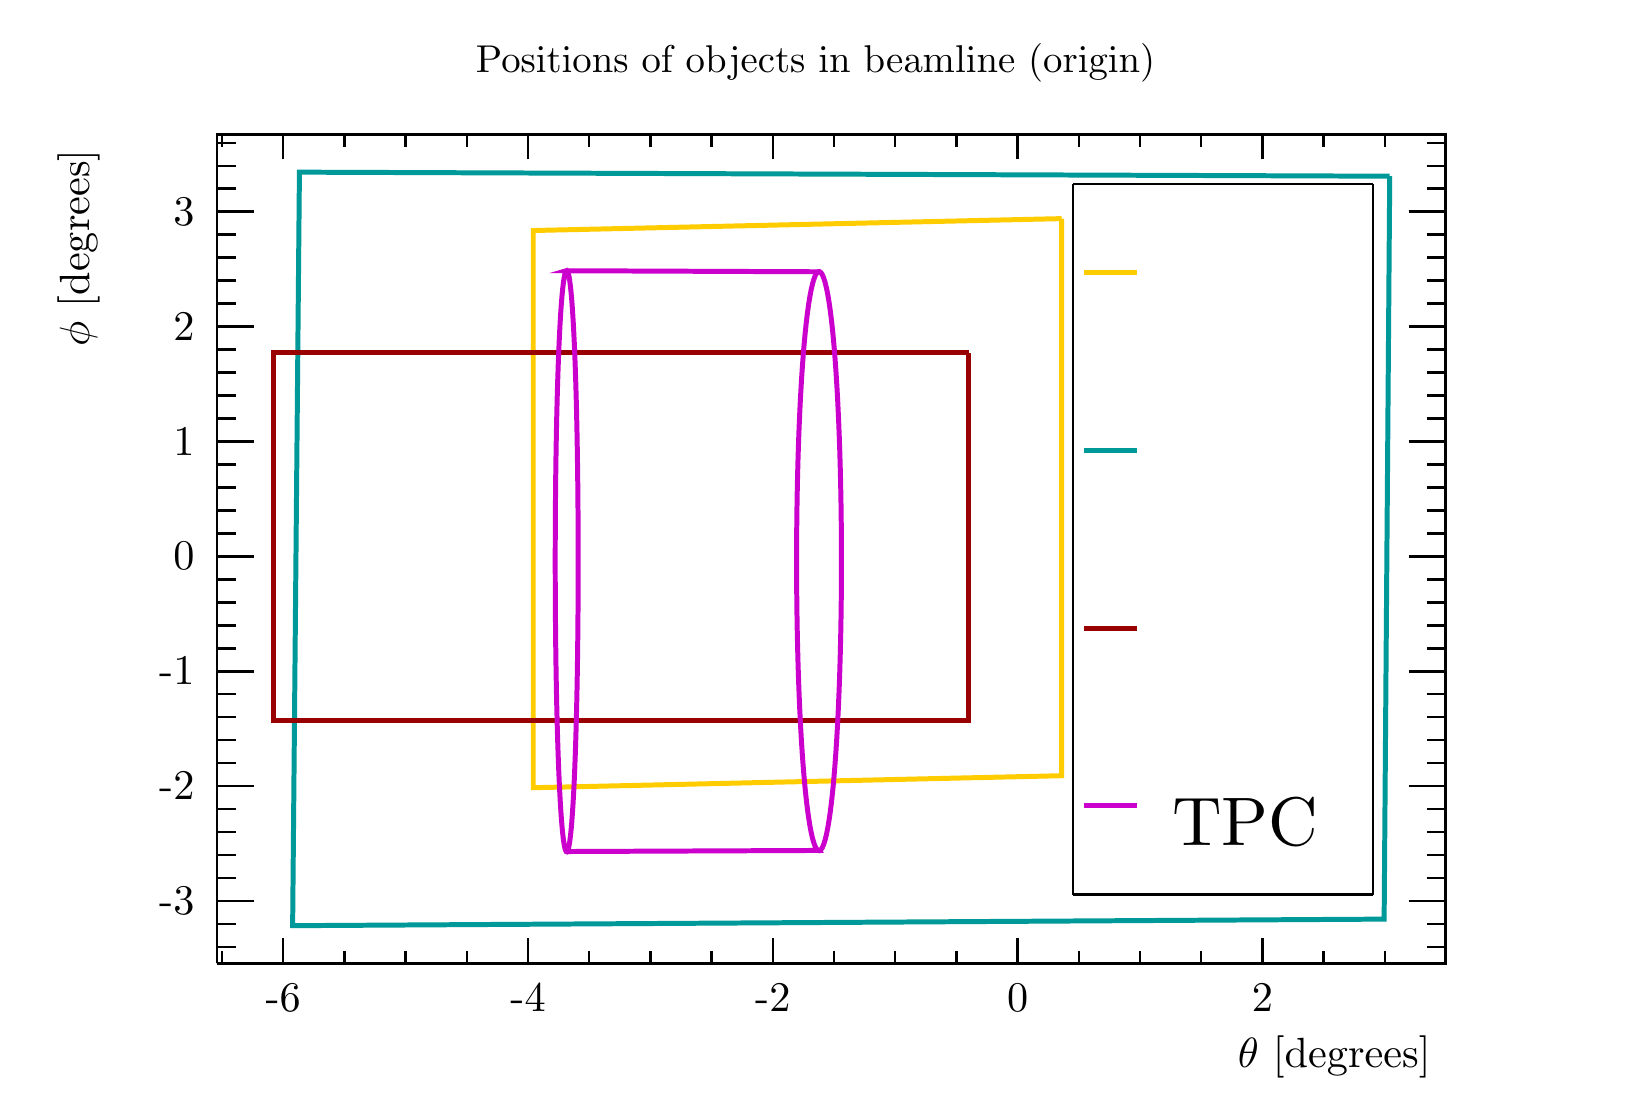
\begin{tikzpicture}
\pgfdeclareplotmark{cross} {
\pgfpathmoveto{\pgfpoint{-0.3\pgfplotmarksize}{\pgfplotmarksize}}
\pgfpathlineto{\pgfpoint{+0.3\pgfplotmarksize}{\pgfplotmarksize}}
\pgfpathlineto{\pgfpoint{+0.3\pgfplotmarksize}{0.3\pgfplotmarksize}}
\pgfpathlineto{\pgfpoint{+1\pgfplotmarksize}{0.3\pgfplotmarksize}}
\pgfpathlineto{\pgfpoint{+1\pgfplotmarksize}{-0.3\pgfplotmarksize}}
\pgfpathlineto{\pgfpoint{+0.3\pgfplotmarksize}{-0.3\pgfplotmarksize}}
\pgfpathlineto{\pgfpoint{+0.3\pgfplotmarksize}{-1.\pgfplotmarksize}}
\pgfpathlineto{\pgfpoint{-0.3\pgfplotmarksize}{-1.\pgfplotmarksize}}
\pgfpathlineto{\pgfpoint{-0.3\pgfplotmarksize}{-0.3\pgfplotmarksize}}
\pgfpathlineto{\pgfpoint{-1.\pgfplotmarksize}{-0.3\pgfplotmarksize}}
\pgfpathlineto{\pgfpoint{-1.\pgfplotmarksize}{0.3\pgfplotmarksize}}
\pgfpathlineto{\pgfpoint{-0.3\pgfplotmarksize}{0.3\pgfplotmarksize}}
\pgfpathclose
\pgfusepathqstroke
}
\pgfdeclareplotmark{cross*} {
\pgfpathmoveto{\pgfpoint{-0.3\pgfplotmarksize}{\pgfplotmarksize}}
\pgfpathlineto{\pgfpoint{+0.3\pgfplotmarksize}{\pgfplotmarksize}}
\pgfpathlineto{\pgfpoint{+0.3\pgfplotmarksize}{0.3\pgfplotmarksize}}
\pgfpathlineto{\pgfpoint{+1\pgfplotmarksize}{0.3\pgfplotmarksize}}
\pgfpathlineto{\pgfpoint{+1\pgfplotmarksize}{-0.3\pgfplotmarksize}}
\pgfpathlineto{\pgfpoint{+0.3\pgfplotmarksize}{-0.3\pgfplotmarksize}}
\pgfpathlineto{\pgfpoint{+0.3\pgfplotmarksize}{-1.\pgfplotmarksize}}
\pgfpathlineto{\pgfpoint{-0.3\pgfplotmarksize}{-1.\pgfplotmarksize}}
\pgfpathlineto{\pgfpoint{-0.3\pgfplotmarksize}{-0.3\pgfplotmarksize}}
\pgfpathlineto{\pgfpoint{-1.\pgfplotmarksize}{-0.3\pgfplotmarksize}}
\pgfpathlineto{\pgfpoint{-1.\pgfplotmarksize}{0.3\pgfplotmarksize}}
\pgfpathlineto{\pgfpoint{-0.3\pgfplotmarksize}{0.3\pgfplotmarksize}}
\pgfpathclose
\pgfusepathqfillstroke
}
\pgfdeclareplotmark{newstar} {
\pgfpathmoveto{\pgfqpoint{0pt}{\pgfplotmarksize}}
\pgfpathlineto{\pgfqpointpolar{44}{0.5\pgfplotmarksize}}
\pgfpathlineto{\pgfqpointpolar{18}{\pgfplotmarksize}}
\pgfpathlineto{\pgfqpointpolar{-20}{0.5\pgfplotmarksize}}
\pgfpathlineto{\pgfqpointpolar{-54}{\pgfplotmarksize}}
\pgfpathlineto{\pgfqpointpolar{-90}{0.5\pgfplotmarksize}}
\pgfpathlineto{\pgfqpointpolar{234}{\pgfplotmarksize}}
\pgfpathlineto{\pgfqpointpolar{198}{0.5\pgfplotmarksize}}
\pgfpathlineto{\pgfqpointpolar{162}{\pgfplotmarksize}}
\pgfpathlineto{\pgfqpointpolar{134}{0.5\pgfplotmarksize}}
\pgfpathclose
\pgfusepathqstroke
}
\pgfdeclareplotmark{newstar*} {
\pgfpathmoveto{\pgfqpoint{0pt}{\pgfplotmarksize}}
\pgfpathlineto{\pgfqpointpolar{44}{0.5\pgfplotmarksize}}
\pgfpathlineto{\pgfqpointpolar{18}{\pgfplotmarksize}}
\pgfpathlineto{\pgfqpointpolar{-20}{0.5\pgfplotmarksize}}
\pgfpathlineto{\pgfqpointpolar{-54}{\pgfplotmarksize}}
\pgfpathlineto{\pgfqpointpolar{-90}{0.5\pgfplotmarksize}}
\pgfpathlineto{\pgfqpointpolar{234}{\pgfplotmarksize}}
\pgfpathlineto{\pgfqpointpolar{198}{0.5\pgfplotmarksize}}
\pgfpathlineto{\pgfqpointpolar{162}{\pgfplotmarksize}}
\pgfpathlineto{\pgfqpointpolar{134}{0.5\pgfplotmarksize}}
\pgfpathclose
\pgfusepathqfillstroke
}
\definecolor{c}{rgb}{1,1,1};
\draw [color=c, fill=c] (0,0) rectangle (20,13.4957);
\draw [color=c, fill=c] (2.4,1.61948) rectangle (18,12.1461);
\definecolor{c}{rgb}{0,0,0};
\draw [c,line width=0.9] (2.4,1.61948) -- (2.4,12.1461) -- (18,12.1461) -- (18,1.61948) -- (2.4,1.61948);
\definecolor{c}{rgb}{1,1,1};
\draw [color=c, fill=c] (2.4,1.61948) rectangle (18,12.1461);
\definecolor{c}{rgb}{0,0,0};
\draw [c,line width=0.9] (2.4,1.61948) -- (2.4,12.1461) -- (18,12.1461) -- (18,1.61948) -- (2.4,1.61948);
\draw [c,line width=0.9] (2.4,1.61948) -- (18,1.61948);
\draw [c,line width=0.9] (3.23864,1.93528) -- (3.23864,1.61948);
\draw [c,line width=0.9] (4.01586,1.77738) -- (4.01586,1.61948);
\draw [c,line width=0.9] (4.79308,1.77738) -- (4.79308,1.61948);
\draw [c,line width=0.9] (5.5703,1.77738) -- (5.5703,1.61948);
\draw [c,line width=0.9] (6.34753,1.93528) -- (6.34753,1.61948);
\draw [c,line width=0.9] (7.12475,1.77738) -- (7.12475,1.61948);
\draw [c,line width=0.9] (7.90197,1.77738) -- (7.90197,1.61948);
\draw [c,line width=0.9] (8.67919,1.77738) -- (8.67919,1.61948);
\draw [c,line width=0.9] (9.45641,1.93528) -- (9.45641,1.61948);
\draw [c,line width=0.9] (10.2336,1.77738) -- (10.2336,1.61948);
\draw [c,line width=0.9] (11.0109,1.77738) -- (11.0109,1.61948);
\draw [c,line width=0.9] (11.7881,1.77738) -- (11.7881,1.61948);
\draw [c,line width=0.9] (12.5653,1.93528) -- (12.5653,1.61948);
\draw [c,line width=0.9] (13.3425,1.77738) -- (13.3425,1.61948);
\draw [c,line width=0.9] (14.1197,1.77738) -- (14.1197,1.61948);
\draw [c,line width=0.9] (14.897,1.77738) -- (14.897,1.61948);
\draw [c,line width=0.9] (15.6742,1.93528) -- (15.6742,1.61948);
\draw [c,line width=0.9] (3.23864,1.93528) -- (3.23864,1.61948);
\draw [c,line width=0.9] (2.46142,1.77738) -- (2.46142,1.61948);
\draw [c,line width=0.9] (15.6742,1.93528) -- (15.6742,1.61948);
\draw [c,line width=0.9] (16.4514,1.77738) -- (16.4514,1.61948);
\draw [c,line width=0.9] (17.2286,1.77738) -- (17.2286,1.61948);
\draw [anchor=base] (3.23864,1.01218) node[scale=1.52731, color=c, rotate=0]{-6};
\draw [anchor=base] (6.34753,1.01218) node[scale=1.52731, color=c, rotate=0]{-4};
\draw [anchor=base] (9.45641,1.01218) node[scale=1.52731, color=c, rotate=0]{-2};
\draw [anchor=base] (12.5653,1.01218) node[scale=1.52731, color=c, rotate=0]{0};
\draw [anchor=base] (15.6742,1.01218) node[scale=1.52731, color=c, rotate=0]{2};
\draw [anchor= east] (18,0.431862) node[scale=1.52731, color=c, rotate=0]{$ \theta$ [degrees]};
\draw [c,line width=0.9] (2.4,12.1461) -- (18,12.1461);
\draw [c,line width=0.9] (3.23864,11.8303) -- (3.23864,12.1461);
\draw [c,line width=0.9] (4.01586,11.9882) -- (4.01586,12.1461);
\draw [c,line width=0.9] (4.79308,11.9882) -- (4.79308,12.1461);
\draw [c,line width=0.9] (5.5703,11.9882) -- (5.5703,12.1461);
\draw [c,line width=0.9] (6.34753,11.8303) -- (6.34753,12.1461);
\draw [c,line width=0.9] (7.12475,11.9882) -- (7.12475,12.1461);
\draw [c,line width=0.9] (7.90197,11.9882) -- (7.90197,12.1461);
\draw [c,line width=0.9] (8.67919,11.9882) -- (8.67919,12.1461);
\draw [c,line width=0.9] (9.45641,11.8303) -- (9.45641,12.1461);
\draw [c,line width=0.9] (10.2336,11.9882) -- (10.2336,12.1461);
\draw [c,line width=0.9] (11.0109,11.9882) -- (11.0109,12.1461);
\draw [c,line width=0.9] (11.7881,11.9882) -- (11.7881,12.1461);
\draw [c,line width=0.9] (12.5653,11.8303) -- (12.5653,12.1461);
\draw [c,line width=0.9] (13.3425,11.9882) -- (13.3425,12.1461);
\draw [c,line width=0.9] (14.1197,11.9882) -- (14.1197,12.1461);
\draw [c,line width=0.9] (14.897,11.9882) -- (14.897,12.1461);
\draw [c,line width=0.9] (15.6742,11.8303) -- (15.6742,12.1461);
\draw [c,line width=0.9] (3.23864,11.8303) -- (3.23864,12.1461);
\draw [c,line width=0.9] (2.46142,11.9882) -- (2.46142,12.1461);
\draw [c,line width=0.9] (15.6742,11.8303) -- (15.6742,12.1461);
\draw [c,line width=0.9] (16.4514,11.9882) -- (16.4514,12.1461);
\draw [c,line width=0.9] (17.2286,11.9882) -- (17.2286,12.1461);
\draw [c,line width=0.9] (2.4,1.61948) -- (2.4,12.1461);
\draw [c,line width=0.9] (2.868,2.41096) -- (2.4,2.41096);
\draw [c,line width=0.9] (2.634,2.70278) -- (2.4,2.70278);
\draw [c,line width=0.9] (2.634,2.99459) -- (2.4,2.99459);
\draw [c,line width=0.9] (2.634,3.28641) -- (2.4,3.28641);
\draw [c,line width=0.9] (2.634,3.57822) -- (2.4,3.57822);
\draw [c,line width=0.9] (2.868,3.87004) -- (2.4,3.87004);
\draw [c,line width=0.9] (2.634,4.16185) -- (2.4,4.16185);
\draw [c,line width=0.9] (2.634,4.45367) -- (2.4,4.45367);
\draw [c,line width=0.9] (2.634,4.74548) -- (2.4,4.74548);
\draw [c,line width=0.9] (2.634,5.0373) -- (2.4,5.0373);
\draw [c,line width=0.9] (2.868,5.32911) -- (2.4,5.32911);
\draw [c,line width=0.9] (2.634,5.62093) -- (2.4,5.62093);
\draw [c,line width=0.9] (2.634,5.91274) -- (2.4,5.91274);
\draw [c,line width=0.9] (2.634,6.20456) -- (2.4,6.20456);
\draw [c,line width=0.9] (2.634,6.49638) -- (2.4,6.49638);
\draw [c,line width=0.9] (2.868,6.78819) -- (2.4,6.78819);
\draw [c,line width=0.9] (2.634,7.08001) -- (2.4,7.08001);
\draw [c,line width=0.9] (2.634,7.37182) -- (2.4,7.37182);
\draw [c,line width=0.9] (2.634,7.66364) -- (2.4,7.66364);
\draw [c,line width=0.9] (2.634,7.95545) -- (2.4,7.95545);
\draw [c,line width=0.9] (2.868,8.24727) -- (2.4,8.24727);
\draw [c,line width=0.9] (2.634,8.53908) -- (2.4,8.53908);
\draw [c,line width=0.9] (2.634,8.8309) -- (2.4,8.8309);
\draw [c,line width=0.9] (2.634,9.12271) -- (2.4,9.12271);
\draw [c,line width=0.9] (2.634,9.41453) -- (2.4,9.41453);
\draw [c,line width=0.9] (2.868,9.70634) -- (2.4,9.70634);
\draw [c,line width=0.9] (2.634,9.99816) -- (2.4,9.99816);
\draw [c,line width=0.9] (2.634,10.29) -- (2.4,10.29);
\draw [c,line width=0.9] (2.634,10.5818) -- (2.4,10.5818);
\draw [c,line width=0.9] (2.634,10.8736) -- (2.4,10.8736);
\draw [c,line width=0.9] (2.868,11.1654) -- (2.4,11.1654);
\draw [c,line width=0.9] (2.868,2.41096) -- (2.4,2.41096);
\draw [c,line width=0.9] (2.634,2.11915) -- (2.4,2.11915);
\draw [c,line width=0.9] (2.634,1.82733) -- (2.4,1.82733);
\draw [c,line width=0.9] (2.868,11.1654) -- (2.4,11.1654);
\draw [c,line width=0.9] (2.634,11.4572) -- (2.4,11.4572);
\draw [c,line width=0.9] (2.634,11.749) -- (2.4,11.749);
\draw [c,line width=0.9] (2.634,12.0409) -- (2.4,12.0409);
\draw [anchor= east] (2.3,2.41096) node[scale=1.52731, color=c, rotate=0]{-3};
\draw [anchor= east] (2.3,3.87004) node[scale=1.52731, color=c, rotate=0]{-2};
\draw [anchor= east] (2.3,5.32911) node[scale=1.52731, color=c, rotate=0]{-1};
\draw [anchor= east] (2.3,6.78819) node[scale=1.52731, color=c, rotate=0]{0};
\draw [anchor= east] (2.3,8.24727) node[scale=1.52731, color=c, rotate=0]{1};
\draw [anchor= east] (2.3,9.70634) node[scale=1.52731, color=c, rotate=0]{2};
\draw [anchor= east] (2.3,11.1654) node[scale=1.52731, color=c, rotate=0]{3};
\draw [anchor= east] (0.64,12.1461) node[scale=1.52731, color=c, rotate=90]{$ \phi$ [degrees]};
\draw [c,line width=0.9] (18,1.61948) -- (18,12.1461);
\draw [c,line width=0.9] (17.532,2.41096) -- (18,2.41096);
\draw [c,line width=0.9] (17.766,2.70278) -- (18,2.70278);
\draw [c,line width=0.9] (17.766,2.99459) -- (18,2.99459);
\draw [c,line width=0.9] (17.766,3.28641) -- (18,3.28641);
\draw [c,line width=0.9] (17.766,3.57822) -- (18,3.57822);
\draw [c,line width=0.9] (17.532,3.87004) -- (18,3.87004);
\draw [c,line width=0.9] (17.766,4.16185) -- (18,4.16185);
\draw [c,line width=0.9] (17.766,4.45367) -- (18,4.45367);
\draw [c,line width=0.9] (17.766,4.74548) -- (18,4.74548);
\draw [c,line width=0.9] (17.766,5.0373) -- (18,5.0373);
\draw [c,line width=0.9] (17.532,5.32911) -- (18,5.32911);
\draw [c,line width=0.9] (17.766,5.62093) -- (18,5.62093);
\draw [c,line width=0.9] (17.766,5.91274) -- (18,5.91274);
\draw [c,line width=0.9] (17.766,6.20456) -- (18,6.20456);
\draw [c,line width=0.9] (17.766,6.49638) -- (18,6.49638);
\draw [c,line width=0.9] (17.532,6.78819) -- (18,6.78819);
\draw [c,line width=0.9] (17.766,7.08001) -- (18,7.08001);
\draw [c,line width=0.9] (17.766,7.37182) -- (18,7.37182);
\draw [c,line width=0.9] (17.766,7.66364) -- (18,7.66364);
\draw [c,line width=0.9] (17.766,7.95545) -- (18,7.95545);
\draw [c,line width=0.9] (17.532,8.24727) -- (18,8.24727);
\draw [c,line width=0.9] (17.766,8.53908) -- (18,8.53908);
\draw [c,line width=0.9] (17.766,8.8309) -- (18,8.8309);
\draw [c,line width=0.9] (17.766,9.12271) -- (18,9.12271);
\draw [c,line width=0.9] (17.766,9.41453) -- (18,9.41453);
\draw [c,line width=0.9] (17.532,9.70634) -- (18,9.70634);
\draw [c,line width=0.9] (17.766,9.99816) -- (18,9.99816);
\draw [c,line width=0.9] (17.766,10.29) -- (18,10.29);
\draw [c,line width=0.9] (17.766,10.5818) -- (18,10.5818);
\draw [c,line width=0.9] (17.766,10.8736) -- (18,10.8736);
\draw [c,line width=0.9] (17.532,11.1654) -- (18,11.1654);
\draw [c,line width=0.9] (17.532,2.41096) -- (18,2.41096);
\draw [c,line width=0.9] (17.766,2.11915) -- (18,2.11915);
\draw [c,line width=0.9] (17.766,1.82733) -- (18,1.82733);
\draw [c,line width=0.9] (17.532,11.1654) -- (18,11.1654);
\draw [c,line width=0.9] (17.766,11.4572) -- (18,11.4572);
\draw [c,line width=0.9] (17.766,11.749) -- (18,11.749);
\draw [c,line width=0.9] (17.766,12.0409) -- (18,12.0409);
\definecolor{c}{rgb}{1,0.8,0};
\draw [c,line width=1.8] (13.123,11.0775) -- (13.123,4.00254) -- (6.41361,3.85009) -- (6.41361,10.9264) -- (13.123,11.0775);
\definecolor{c}{rgb}{0,0.6,0.6};
\draw [c,line width=1.8] (17.2909,11.6163) -- (3.44422,11.6676) -- (3.35799,2.09797) -- (17.22,2.18131) -- (17.2909,11.6163);
\definecolor{c}{rgb}{0.6,0,0};
\draw [c,line width=1.8] (11.9426,9.37206) -- (3.10909,9.37206) -- (3.10909,4.70729) -- (11.9426,4.70729) -- (11.9426,9.37206);
\definecolor{c}{rgb}{0.8,0,0.8};
\draw [c,line width=1.8] (6.83226,10.4157) -- (6.82314,10.3986) -- (6.81412,10.3672) -- (6.80521,10.3217) -- (6.79645,10.2624) -- (6.78788,10.1897) -- (6.77953,10.104) -- (6.77142,10.0055) -- (6.76359,9.89494) -- (6.75605,9.77263) --
 (6.74885,9.63914) -- (6.74199,9.49505) -- (6.73552,9.34093) -- (6.72943,9.17739) -- (6.72376,9.00508) -- (6.71852,8.82465) -- (6.71374,8.63678) -- (6.70941,8.44217) -- (6.70557,8.24152) -- (6.70221,8.03556) -- (6.69935,7.82503) -- (6.697,7.61067) --
 (6.69517,7.39324) -- (6.69385,7.17349) -- (6.69306,6.9522) -- (6.6928,6.73012) -- (6.69306,6.50804) -- (6.69385,6.28672) -- (6.69517,6.06693) -- (6.697,5.84944) -- (6.69935,5.635) -- (6.70221,5.42438) -- (6.70557,5.21831) -- (6.70941,5.01753) --
 (6.71374,4.82277) -- (6.71852,4.63474) -- (6.72376,4.45413) -- (6.72943,4.28163) -- (6.73552,4.11789) -- (6.74199,3.96355) -- (6.74885,3.81922) -- (6.75605,3.68549) -- (6.76359,3.56292) -- (6.77142,3.45203) -- (6.77953,3.35333) -- (6.78788,3.26727)
 -- (6.79645,3.19426) -- (6.80521,3.13469) -- (6.81412,3.08889) -- (6.82314,3.05715) -- (6.83226,3.0397) -- (6.84142,3.03673) -- (6.8506,3.04837) -- (6.85976,3.07469) -- (6.86885,3.11572) -- (6.87785,3.17139) -- (6.88671,3.24161) -- (6.8954,3.3262)
 -- (6.90388,3.42493) -- (6.91211,3.53747) -- (6.92006,3.66348) -- (6.92769,3.80249) -- (6.93496,3.95402) -- (6.94184,4.11749) -- (6.9483,4.29226) -- (6.95431,4.47764) -- (6.95985,4.67288) -- (6.96487,4.87717) -- (6.96936,5.08963) -- (6.9733,5.30937)
 -- (6.97667,5.53544) -- (6.97945,5.76682) -- (6.98163,6.00252) -- (6.98319,6.24147) -- (6.98413,6.4826) -- (6.98444,6.72484) -- (6.98413,6.96709) -- (6.98319,7.20826) -- (6.98163,7.44728) -- (6.97945,7.68305) -- (6.97667,7.91455) -- (6.9733,8.14075)
 -- (6.96936,8.36064) -- (6.96487,8.57329) -- (6.95985,8.77777) -- (6.95431,8.97322) -- (6.9483,9.15884) -- (6.94184,9.33386) -- (6.93496,9.49759) -- (6.92769,9.6494) -- (6.92006,9.7887) -- (6.91211,9.91501) -- (6.90388,10.0279) -- (6.8954,10.1269)
 -- (6.88671,10.2118) -- (6.87785,10.2824) -- (6.86885,10.3384) -- (6.85976,10.3797) -- (6.8506,10.4064) -- (6.84142,10.4184) -- (6.83226,10.4157) -- (10.0306,10.4025);
\draw [c,line width=1.8] (10.0306,3.05337) -- (10.0485,3.05045) -- (10.0665,3.06209) -- (10.0843,3.08835) -- (10.1021,3.12926) -- (10.1197,3.18477) -- (10.137,3.25476) -- (10.154,3.33907) -- (10.1705,3.43746) -- (10.1866,3.54962) -- (10.2022,3.67518)
 -- (10.2171,3.8137) -- (10.2313,3.96468) -- (10.2447,4.12756) -- (10.2573,4.30169) -- (10.2691,4.48639) -- (10.2799,4.6809) -- (10.2897,4.88442) -- (10.2985,5.09609) -- (10.3062,5.315) -- (10.3127,5.54021) -- (10.3182,5.77072) -- (10.3224,6.00552)
 -- (10.3255,6.24356) -- (10.3273,6.48377) -- (10.3279,6.72508) -- (10.3273,6.96641) -- (10.3255,7.20666) -- (10.3224,7.44476) -- (10.3182,7.67964) -- (10.3127,7.91026) -- (10.3062,8.1356) -- (10.2985,8.35466) -- (10.2897,8.56651) --
 (10.2799,8.77022) -- (10.2691,8.96495) -- (10.2573,9.14988) -- (10.2447,9.32426) -- (10.2313,9.4874) -- (10.2171,9.63865) -- (10.2022,9.77747) -- (10.1866,9.90332) -- (10.1705,10.0158) -- (10.154,10.1145) -- (10.137,10.1991) -- (10.1197,10.2695) --
 (10.1021,10.3253) -- (10.0843,10.3665) -- (10.0665,10.3931) -- (10.0485,10.4051) -- (10.0306,10.4025) -- (10.0128,10.3855) -- (9.99516,10.3542) -- (9.97776,10.3089) -- (9.96065,10.2499) -- (9.9439,10.1775) -- (9.92757,10.0921) -- (9.91173,9.99402)
 -- (9.89642,9.88383) -- (9.8817,9.76198) -- (9.86762,9.62899) -- (9.85423,9.48543) -- (9.84156,9.33188) -- (9.82967,9.16894) -- (9.81859,8.99725) -- (9.80836,8.81747) -- (9.799,8.63027) -- (9.79055,8.43635) -- (9.78303,8.23641) -- (9.77647,8.03118)
 -- (9.77088,7.82139) -- (9.76629,7.60779) -- (9.7627,7.39112) -- (9.76013,7.17214) -- (9.75859,6.95162) -- (9.75807,6.73033) -- (9.75859,6.50902) -- (9.76013,6.28848) -- (9.7627,6.06946) -- (9.76629,5.85273) -- (9.77088,5.63905) -- (9.77647,5.42916)
 -- (9.78303,5.22382) -- (9.79055,5.02376) -- (9.799,4.82969) -- (9.80836,4.64234) -- (9.81859,4.46238) -- (9.82967,4.2905) -- (9.84156,4.12736) -- (9.85423,3.97358) -- (9.86762,3.82979) -- (9.8817,3.69656) -- (9.89642,3.57445) -- (9.91173,3.46399)
 -- (9.92757,3.36567) -- (9.9439,3.27994) -- (9.96065,3.20723) -- (9.97776,3.14791) -- (9.99516,3.10231) -- (10.0128,3.07072) -- (10.0306,3.05337) -- (6.83226,3.0397);
\definecolor{c}{rgb}{1,1,1};
\draw [color=c, fill=c] (2,12.686) rectangle (18,13.4282);
\definecolor{c}{rgb}{0,0,0};
\draw (10,13.0571) node[scale=1.40004, color=c, rotate=0]{Positions of objects in beamline (\SOne origin)};
\definecolor{c}{rgb}{1,1,1};
\draw [color=c, fill=c] (13.2665,2.49284) rectangle (17.0774,11.5186);
\definecolor{c}{rgb}{0,0,0};
\draw [c,line width=0.9] (13.2665,2.49284) -- (17.0774,2.49284);
\draw [c,line width=0.9] (17.0774,2.49284) -- (17.0774,11.5186);
\draw [c,line width=0.9] (17.0774,11.5186) -- (13.2665,11.5186);
\draw [c,line width=0.9] (13.2665,11.5186) -- (13.2665,2.49284);
\draw [anchor=base west] (14.2192,9.8827) node[scale=2.48189, color=c, rotate=0]{\STwo};
\definecolor{c}{rgb}{1,0.8,0};
\draw [c,line width=1.8] (13.4094,10.3904) -- (14.0763,10.3904);
\definecolor{c}{rgb}{0,0,0};
\draw [anchor=base west] (14.2192,7.62625) node[scale=2.48189, color=c, rotate=0]{\SThree};
\definecolor{c}{rgb}{0,0.6,0.6};
\draw [c,line width=1.8] (13.4094,8.13395) -- (14.0763,8.13395);
\definecolor{c}{rgb}{0,0,0};
\draw [anchor=base west] (14.2192,5.36981) node[scale=2.48189, color=c, rotate=0]{\SFour};
\definecolor{c}{rgb}{0.6,0,0};
\draw [c,line width=1.8] (13.4094,5.87751) -- (14.0763,5.87751);
\definecolor{c}{rgb}{0,0,0};
\draw [anchor=base west] (14.2192,3.11336) node[scale=2.48189, color=c, rotate=0]{TPC};
\definecolor{c}{rgb}{0.8,0,0.8};
\draw [c,line width=1.8] (13.4094,3.62106) -- (14.0763,3.62106);
\end{tikzpicture}

  \end{adjustbox}
  \caption[Angular distribution of objects in the T10 beamline]{Angular distribution of objects within the T10 beamline. The origin here is at \SOne.}
  \label{fig:angDistS1}
\end{figure}

\begin{table}
  \centering
  \caption[Angular extent of components within the T10 beamline with \SOne as the origin]{Angular extent of components within the T10 beamline with \SOne as the origin.}
  \label{tab:angDistS1}
  \begin{tabular}{c c c c c}
    \hline
    \hline
    Object & $\theta_{\text{min}}$ & $\theta_{\text{max}}$ & $\phi_{\text{min}}$ & $\theta_{\text{max}}$ \\
    \hline
    \STwo & $\ang{-3.96} \pm \ang{0.03}$ & $\ang{0.36} \pm \ang{0.03}$ & $\ang{-2.01} \pm \ang{0.03}$ & $\ang{2.94} \pm \ang{0.03}$\\
    \SThree & $\ang{-5.923} \pm \ang{0.004}$ & $\ang{3.040} \pm \ang{0.004}$ & $\ang{-3.215} \pm \ang{0.004}$ & $\ang{3.344} \pm \ang{0.004}$ \\
    \SFour & $\ang{-6.083} \pm \ang{0.003}$ & $\ang{-0.401} \pm \ang{0.003}$ & $\ang{-1.426} \pm \ang{0.003}$ & $\ang{1.771} \pm \ang{0.003}$ \\
    TPC US face & $\ang{-3.59} \pm \ang{0.01}$ & $\ang{-1.44} \pm \ang{0.01}$ & $\ang{-2.66} \pm \ang{0.01}$ & $\ang{2.58} \pm \ang{0.01}$ \\
    TPC DS face & $\ang{-3.778} \pm \ang{0.009}$ & $\ang{-1.806} \pm \ang{0.009}$ & $\ang{-2.440} \pm \ang{0.009}$ & $\ang{2.361} \pm \ang{0.009}$ \\
    \hline 
  \end{tabular}
\end{table}

\citefig{fig:beamlinePics} shows images of the beamline with the various components of the ToF systems as well as the HPTPC and moderator blocks labelled.
In this particular image, all four moderator blocks are placed on the tripod stand.

\begin{figure}[h]
  \centering
  \includegraphics[width=\linewidth]{files/figures/hptpc_beam_flux/S1S2S3S4}
  \caption[Images of the test beam setup with various objects labelled]{Images of the T10 beamline with the apparatus used in the beam test labelled. Left: the downstream part of the beamline. Right: The upstream part of the beamline. Image from~\cite{beampaper}.}
  \label{fig:beamlinePics}
\end{figure}

\SThree and \SFour each have their own independent DAQ systems which process data from \SOne and \STwo plus either \SThree or \SFour.
The data from these two systems is synchronised offline using a signal from the PS indicating the arrival of a beam spill which is recorded by both DAQs.

T10 receives $1-3$ spills from the PS every supercycle, which has a normal duration of \SI{33}{\second}.
The duration of each of these spills is approximately \SI{0.4}{\second}.
The minimum separation in time of these spills is \SI{1}{\second} which means that the beam spill arrival signal has a frequency of less than \SI{1}{\hertz}.
This means that spills in the two DAQs can be matched by using this signal in combination with the DAQ file timestamps.

\citetab{tab:nSpills} shows the number of recorded spills used for each moderator block configuration for the variable block analysis.
One can see that significantly more spills are recorded in the 4 block configuration.
This is because this is the configuration that was used for the majority of the beam test.

\begin{table}
  \caption[Number of recorded spills for each moderator block configuration used in T10 beam flux analysis]{Number of recorded spills for each moderator block configuration used in T10 beam flux analysis}
  \label{tab:nSpills}
  \begin{tabular}{c c}
    \hline
    \hline
    Number of moderator blocks & Recorded spills \\
    \hline
    0 & 257 \\
    1 & 254 \\
    2 & 267 \\
    3 & 220 \\
    4 & 3884 \\
    \hline
  \end{tabular}
\end{table}

\subsection{The upstream beam counters (\SOne and \STwo)}
\label{sec:hptpc_beam_flux:overview:s1s2}

The \SOne beam counter consists of a cross formed from two pieces of plastic scintillator and is shown in the left hand image of \citefig{fig:s1s2Pic}.
This cross measures \SI{40 x 40 x 5}{\milli\metre} and is attached to four 1'' Hamamatsu Photonics R4998 PMTs at each end which are used to read out the light signals.

\begin{figure}[h]
  \centering
  \includegraphics[width=.7\linewidth]{files/figures/hptpc_beam_flux/S1S2FrontOn}
  \caption[The upstream beam counters \SOne and \STwo]{Images of the upstream beam counters \SOne (left) and \STwo (right) from~\cite{beampaper}.}
  \label{fig:s1s2Pic}
\end{figure}

The time resolution of the \SOne beam counter is measured using the DAQ of the upstream ToF and found to be around \SI{30}{\pico\second}.
This measurement is made by taking the average distribution of the four PMT hit times. However, because this measurement is not centred at zero, we instead calculate the quantity
\begin{equation}
  t_{\text{ave}} = \frac{1}{4} ((t_{\text{PMT1}}+t_{\text{PMT2}}) - (t_{\text{PMT3}}+t_{\text{PMT4}}))
  \label{eq:tAve}
\end{equation}
where the $t_{\text{PMT}n}$ refer to the four PMTs used to read out \SOne.
This quantity has the same spread as the average hit time but is centred at zero.
An example of the distribution produced is shown in \citefig{fig:s1Res} which contains the data from one run.

\begin{figure}[h]
  \begin{adjustbox}{max totalsize=.7\textwidth, center}
    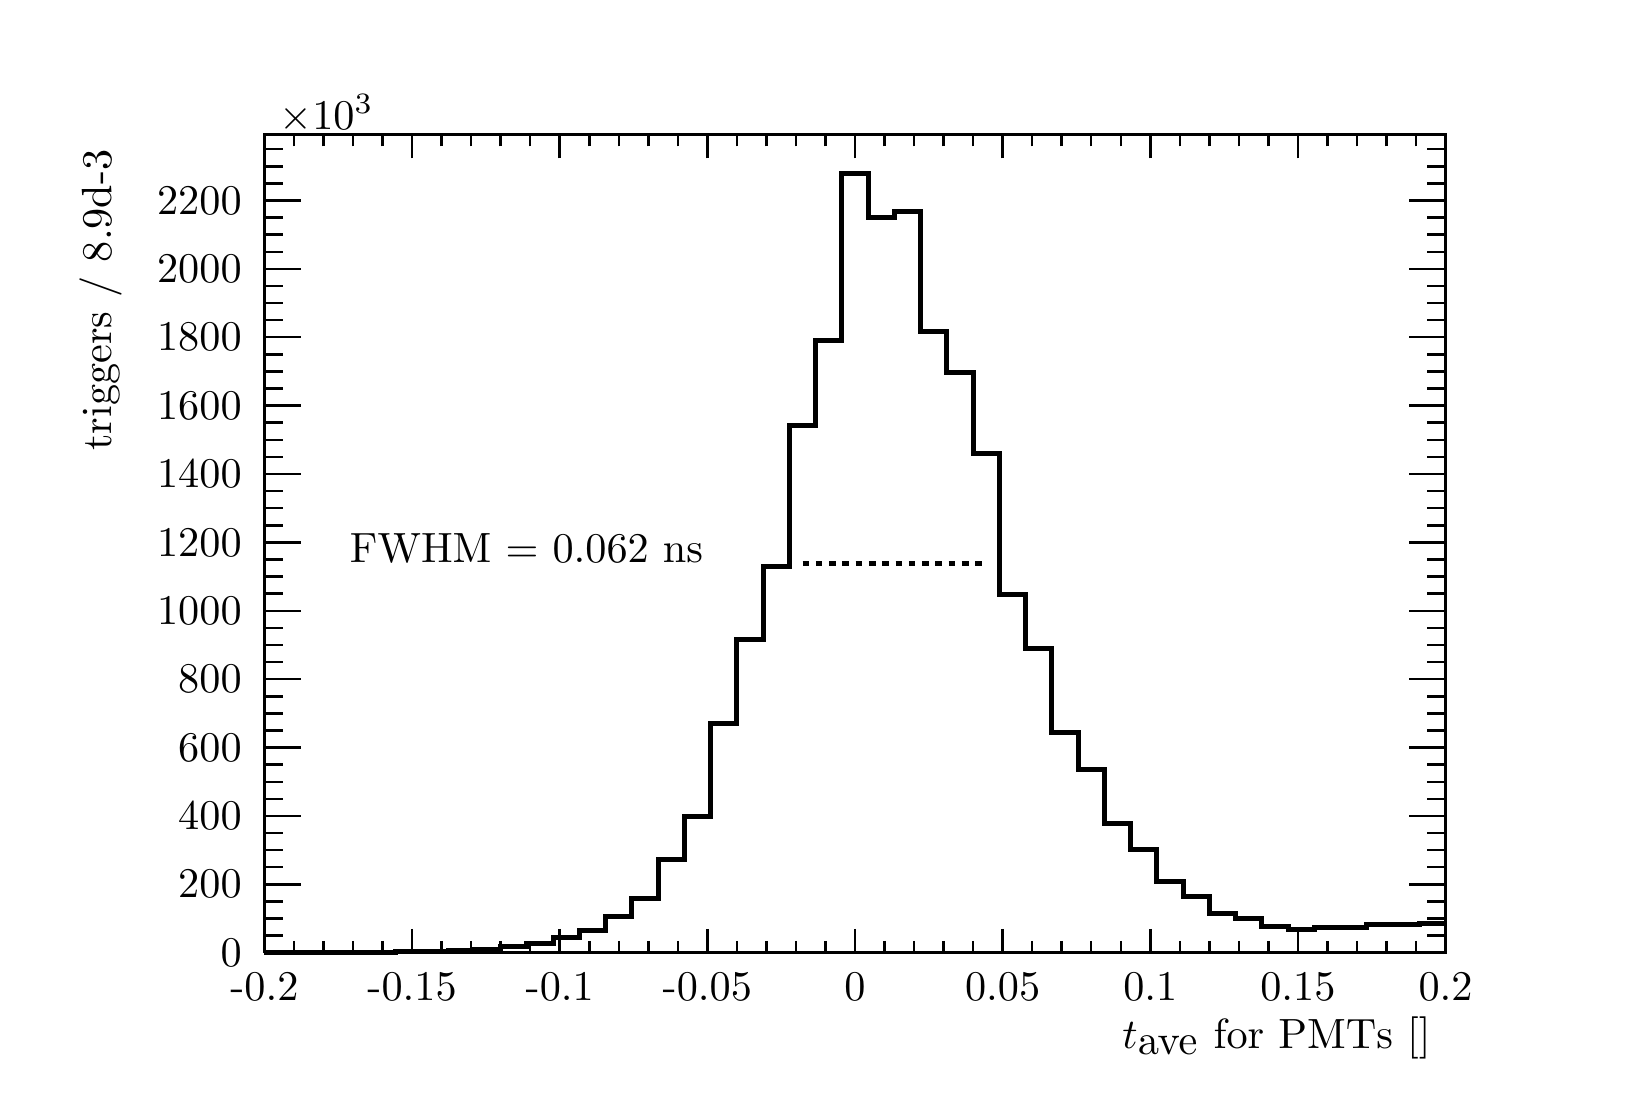
\begin{tikzpicture}
\pgfdeclareplotmark{cross} {
\pgfpathmoveto{\pgfpoint{-0.3\pgfplotmarksize}{\pgfplotmarksize}}
\pgfpathlineto{\pgfpoint{+0.3\pgfplotmarksize}{\pgfplotmarksize}}
\pgfpathlineto{\pgfpoint{+0.3\pgfplotmarksize}{0.3\pgfplotmarksize}}
\pgfpathlineto{\pgfpoint{+1\pgfplotmarksize}{0.3\pgfplotmarksize}}
\pgfpathlineto{\pgfpoint{+1\pgfplotmarksize}{-0.3\pgfplotmarksize}}
\pgfpathlineto{\pgfpoint{+0.3\pgfplotmarksize}{-0.3\pgfplotmarksize}}
\pgfpathlineto{\pgfpoint{+0.3\pgfplotmarksize}{-1.\pgfplotmarksize}}
\pgfpathlineto{\pgfpoint{-0.3\pgfplotmarksize}{-1.\pgfplotmarksize}}
\pgfpathlineto{\pgfpoint{-0.3\pgfplotmarksize}{-0.3\pgfplotmarksize}}
\pgfpathlineto{\pgfpoint{-1.\pgfplotmarksize}{-0.3\pgfplotmarksize}}
\pgfpathlineto{\pgfpoint{-1.\pgfplotmarksize}{0.3\pgfplotmarksize}}
\pgfpathlineto{\pgfpoint{-0.3\pgfplotmarksize}{0.3\pgfplotmarksize}}
\pgfpathclose
\pgfusepathqstroke
}
\pgfdeclareplotmark{cross*} {
\pgfpathmoveto{\pgfpoint{-0.3\pgfplotmarksize}{\pgfplotmarksize}}
\pgfpathlineto{\pgfpoint{+0.3\pgfplotmarksize}{\pgfplotmarksize}}
\pgfpathlineto{\pgfpoint{+0.3\pgfplotmarksize}{0.3\pgfplotmarksize}}
\pgfpathlineto{\pgfpoint{+1\pgfplotmarksize}{0.3\pgfplotmarksize}}
\pgfpathlineto{\pgfpoint{+1\pgfplotmarksize}{-0.3\pgfplotmarksize}}
\pgfpathlineto{\pgfpoint{+0.3\pgfplotmarksize}{-0.3\pgfplotmarksize}}
\pgfpathlineto{\pgfpoint{+0.3\pgfplotmarksize}{-1.\pgfplotmarksize}}
\pgfpathlineto{\pgfpoint{-0.3\pgfplotmarksize}{-1.\pgfplotmarksize}}
\pgfpathlineto{\pgfpoint{-0.3\pgfplotmarksize}{-0.3\pgfplotmarksize}}
\pgfpathlineto{\pgfpoint{-1.\pgfplotmarksize}{-0.3\pgfplotmarksize}}
\pgfpathlineto{\pgfpoint{-1.\pgfplotmarksize}{0.3\pgfplotmarksize}}
\pgfpathlineto{\pgfpoint{-0.3\pgfplotmarksize}{0.3\pgfplotmarksize}}
\pgfpathclose
\pgfusepathqfillstroke
}
\pgfdeclareplotmark{newstar} {
\pgfpathmoveto{\pgfqpoint{0pt}{\pgfplotmarksize}}
\pgfpathlineto{\pgfqpointpolar{44}{0.5\pgfplotmarksize}}
\pgfpathlineto{\pgfqpointpolar{18}{\pgfplotmarksize}}
\pgfpathlineto{\pgfqpointpolar{-20}{0.5\pgfplotmarksize}}
\pgfpathlineto{\pgfqpointpolar{-54}{\pgfplotmarksize}}
\pgfpathlineto{\pgfqpointpolar{-90}{0.5\pgfplotmarksize}}
\pgfpathlineto{\pgfqpointpolar{234}{\pgfplotmarksize}}
\pgfpathlineto{\pgfqpointpolar{198}{0.5\pgfplotmarksize}}
\pgfpathlineto{\pgfqpointpolar{162}{\pgfplotmarksize}}
\pgfpathlineto{\pgfqpointpolar{134}{0.5\pgfplotmarksize}}
\pgfpathclose
\pgfusepathqstroke
}
\pgfdeclareplotmark{newstar*} {
\pgfpathmoveto{\pgfqpoint{0pt}{\pgfplotmarksize}}
\pgfpathlineto{\pgfqpointpolar{44}{0.5\pgfplotmarksize}}
\pgfpathlineto{\pgfqpointpolar{18}{\pgfplotmarksize}}
\pgfpathlineto{\pgfqpointpolar{-20}{0.5\pgfplotmarksize}}
\pgfpathlineto{\pgfqpointpolar{-54}{\pgfplotmarksize}}
\pgfpathlineto{\pgfqpointpolar{-90}{0.5\pgfplotmarksize}}
\pgfpathlineto{\pgfqpointpolar{234}{\pgfplotmarksize}}
\pgfpathlineto{\pgfqpointpolar{198}{0.5\pgfplotmarksize}}
\pgfpathlineto{\pgfqpointpolar{162}{\pgfplotmarksize}}
\pgfpathlineto{\pgfqpointpolar{134}{0.5\pgfplotmarksize}}
\pgfpathclose
\pgfusepathqfillstroke
}
\definecolor{c}{rgb}{1,1,1};
\draw [color=c, fill=c] (0,0) rectangle (20,13.4957);
\draw [color=c, fill=c] (3,1.75444) rectangle (18,12.1461);
\definecolor{c}{rgb}{0,0,0};
\draw [c,line width=0.9] (3,1.75444) -- (3,12.1461) -- (18,12.1461) -- (18,1.75444) -- (3,1.75444);
\definecolor{c}{rgb}{1,1,1};
\draw [color=c, fill=c] (3,1.75444) rectangle (18,12.1461);
\definecolor{c}{rgb}{0,0,0};
\draw [c,line width=0.9] (3,1.75444) -- (3,12.1461) -- (18,12.1461) -- (18,1.75444) -- (3,1.75444);
\draw [c,line width=1.8] (3,1.75651) -- (3.33333,1.75651) -- (3.33333,1.75672) -- (3.66667,1.75672) -- (3.66667,1.75782) -- (4,1.75782) -- (4,1.75928) -- (4.33333,1.75928) -- (4.33333,1.76265) -- (4.66667,1.76265) -- (4.66667,1.76637) -- (5,1.76637)
 -- (5,1.77413) -- (5.33333,1.77413) -- (5.33333,1.78786) -- (5.66667,1.78786) -- (5.66667,1.80025) -- (6,1.80025) -- (6,1.83002) -- (6.33333,1.83002) -- (6.33333,1.8656) -- (6.66667,1.8656) -- (6.66667,1.94289) -- (7,1.94289) -- (7,2.03217) --
 (7.33333,2.03217) -- (7.33333,2.21951) -- (7.66667,2.21951) -- (7.66667,2.44174) -- (8,2.44174) -- (8,2.9414) -- (8.33333,2.9414) -- (8.33333,3.48698) -- (8.66667,3.48698) -- (8.66667,4.66096) -- (9,4.66096) -- (9,5.73419) -- (9.33333,5.73419) --
 (9.33333,6.66117) -- (9.66667,6.66117) -- (9.66667,8.44555) -- (10,8.44555) -- (10,9.52377) -- (10.3333,9.52377) -- (10.3333,11.6513) -- (10.6667,11.6513) -- (10.6667,11.0943) -- (11,11.0943) -- (11,11.169) -- (11.3333,11.169) -- (11.3333,9.64689)
 -- (11.6667,9.64689) -- (11.6667,9.12428) -- (12,9.12428) -- (12,8.09889) -- (12.3333,8.09889) -- (12.3333,6.29961) -- (12.6667,6.29961) -- (12.6667,5.61671) -- (13,5.61671) -- (13,4.54715) -- (13.3333,4.54715) -- (13.3333,4.0756) --
 (13.6667,4.0756) -- (13.6667,3.39822) -- (14,3.39822) -- (14,3.07106) -- (14.3333,3.07106) -- (14.3333,2.65631) -- (14.6667,2.65631) -- (14.6667,2.46793) -- (15,2.46793) -- (15,2.25342) -- (15.3333,2.25342) -- (15.3333,2.18649) -- (15.6667,2.18649)
 -- (15.6667,2.08911) -- (16,2.08911) -- (16,2.05201) -- (16.3333,2.05201) -- (16.3333,2.07377) -- (16.6667,2.07377) -- (16.6667,2.07323) -- (17,2.07323) -- (17,2.1138) -- (17.3333,2.1138) -- (17.3333,2.11352) -- (17.6667,2.11352) --
 (17.6667,2.12843) -- (18,2.12843);
\draw [c,line width=0.9] (3,1.75444) -- (18,1.75444);
\draw [c,line width=0.9] (3,2.05809) -- (3,1.75444);
\draw [c,line width=0.9] (3.375,1.90627) -- (3.375,1.75444);
\draw [c,line width=0.9] (3.75,1.90627) -- (3.75,1.75444);
\draw [c,line width=0.9] (4.125,1.90627) -- (4.125,1.75444);
\draw [c,line width=0.9] (4.5,1.90627) -- (4.5,1.75444);
\draw [c,line width=0.9] (4.875,2.05809) -- (4.875,1.75444);
\draw [c,line width=0.9] (5.25,1.90627) -- (5.25,1.75444);
\draw [c,line width=0.9] (5.625,1.90627) -- (5.625,1.75444);
\draw [c,line width=0.9] (6,1.90627) -- (6,1.75444);
\draw [c,line width=0.9] (6.375,1.90627) -- (6.375,1.75444);
\draw [c,line width=0.9] (6.75,2.05809) -- (6.75,1.75444);
\draw [c,line width=0.9] (7.125,1.90627) -- (7.125,1.75444);
\draw [c,line width=0.9] (7.5,1.90627) -- (7.5,1.75444);
\draw [c,line width=0.9] (7.875,1.90627) -- (7.875,1.75444);
\draw [c,line width=0.9] (8.25,1.90627) -- (8.25,1.75444);
\draw [c,line width=0.9] (8.625,2.05809) -- (8.625,1.75444);
\draw [c,line width=0.9] (9,1.90627) -- (9,1.75444);
\draw [c,line width=0.9] (9.375,1.90627) -- (9.375,1.75444);
\draw [c,line width=0.9] (9.75,1.90627) -- (9.75,1.75444);
\draw [c,line width=0.9] (10.125,1.90627) -- (10.125,1.75444);
\draw [c,line width=0.9] (10.5,2.05809) -- (10.5,1.75444);
\draw [c,line width=0.9] (10.875,1.90627) -- (10.875,1.75444);
\draw [c,line width=0.9] (11.25,1.90627) -- (11.25,1.75444);
\draw [c,line width=0.9] (11.625,1.90627) -- (11.625,1.75444);
\draw [c,line width=0.9] (12,1.90627) -- (12,1.75444);
\draw [c,line width=0.9] (12.375,2.05809) -- (12.375,1.75444);
\draw [c,line width=0.9] (12.75,1.90627) -- (12.75,1.75444);
\draw [c,line width=0.9] (13.125,1.90627) -- (13.125,1.75444);
\draw [c,line width=0.9] (13.5,1.90627) -- (13.5,1.75444);
\draw [c,line width=0.9] (13.875,1.90627) -- (13.875,1.75444);
\draw [c,line width=0.9] (14.25,2.05809) -- (14.25,1.75444);
\draw [c,line width=0.9] (14.625,1.90627) -- (14.625,1.75444);
\draw [c,line width=0.9] (15,1.90627) -- (15,1.75444);
\draw [c,line width=0.9] (15.375,1.90627) -- (15.375,1.75444);
\draw [c,line width=0.9] (15.75,1.90627) -- (15.75,1.75444);
\draw [c,line width=0.9] (16.125,2.05809) -- (16.125,1.75444);
\draw [c,line width=0.9] (16.5,1.90627) -- (16.5,1.75444);
\draw [c,line width=0.9] (16.875,1.90627) -- (16.875,1.75444);
\draw [c,line width=0.9] (17.25,1.90627) -- (17.25,1.75444);
\draw [c,line width=0.9] (17.625,1.90627) -- (17.625,1.75444);
\draw [c,line width=0.9] (18,2.05809) -- (18,1.75444);
\draw [anchor=base] (3,1.14713) node[scale=1.52731, color=c, rotate=0]{-0.2};
\draw [anchor=base] (4.875,1.14713) node[scale=1.52731, color=c, rotate=0]{-0.15};
\draw [anchor=base] (6.75,1.14713) node[scale=1.52731, color=c, rotate=0]{-0.1};
\draw [anchor=base] (8.625,1.14713) node[scale=1.52731, color=c, rotate=0]{-0.05};
\draw [anchor=base] (10.5,1.14713) node[scale=1.52731, color=c, rotate=0]{0};
\draw [anchor=base] (12.375,1.14713) node[scale=1.52731, color=c, rotate=0]{0.05};
\draw [anchor=base] (14.25,1.14713) node[scale=1.52731, color=c, rotate=0]{0.1};
\draw [anchor=base] (16.125,1.14713) node[scale=1.52731, color=c, rotate=0]{0.15};
\draw [anchor=base] (18,1.14713) node[scale=1.52731, color=c, rotate=0]{0.2};
\draw [anchor= east] (18,0.674785) node[scale=1.52731, color=c, rotate=0]{$t_{\textrm{ave}}$ for \SOne PMTs [\si{\nano\second}]};
\draw [c,line width=0.9] (3,12.1461) -- (18,12.1461);
\draw [c,line width=0.9] (3,11.8425) -- (3,12.1461);
\draw [c,line width=0.9] (3.375,11.9943) -- (3.375,12.1461);
\draw [c,line width=0.9] (3.75,11.9943) -- (3.75,12.1461);
\draw [c,line width=0.9] (4.125,11.9943) -- (4.125,12.1461);
\draw [c,line width=0.9] (4.5,11.9943) -- (4.5,12.1461);
\draw [c,line width=0.9] (4.875,11.8425) -- (4.875,12.1461);
\draw [c,line width=0.9] (5.25,11.9943) -- (5.25,12.1461);
\draw [c,line width=0.9] (5.625,11.9943) -- (5.625,12.1461);
\draw [c,line width=0.9] (6,11.9943) -- (6,12.1461);
\draw [c,line width=0.9] (6.375,11.9943) -- (6.375,12.1461);
\draw [c,line width=0.9] (6.75,11.8425) -- (6.75,12.1461);
\draw [c,line width=0.9] (7.125,11.9943) -- (7.125,12.1461);
\draw [c,line width=0.9] (7.5,11.9943) -- (7.5,12.1461);
\draw [c,line width=0.9] (7.875,11.9943) -- (7.875,12.1461);
\draw [c,line width=0.9] (8.25,11.9943) -- (8.25,12.1461);
\draw [c,line width=0.9] (8.625,11.8425) -- (8.625,12.1461);
\draw [c,line width=0.9] (9,11.9943) -- (9,12.1461);
\draw [c,line width=0.9] (9.375,11.9943) -- (9.375,12.1461);
\draw [c,line width=0.9] (9.75,11.9943) -- (9.75,12.1461);
\draw [c,line width=0.9] (10.125,11.9943) -- (10.125,12.1461);
\draw [c,line width=0.9] (10.5,11.8425) -- (10.5,12.1461);
\draw [c,line width=0.9] (10.875,11.9943) -- (10.875,12.1461);
\draw [c,line width=0.9] (11.25,11.9943) -- (11.25,12.1461);
\draw [c,line width=0.9] (11.625,11.9943) -- (11.625,12.1461);
\draw [c,line width=0.9] (12,11.9943) -- (12,12.1461);
\draw [c,line width=0.9] (12.375,11.8425) -- (12.375,12.1461);
\draw [c,line width=0.9] (12.75,11.9943) -- (12.75,12.1461);
\draw [c,line width=0.9] (13.125,11.9943) -- (13.125,12.1461);
\draw [c,line width=0.9] (13.5,11.9943) -- (13.5,12.1461);
\draw [c,line width=0.9] (13.875,11.9943) -- (13.875,12.1461);
\draw [c,line width=0.9] (14.25,11.8425) -- (14.25,12.1461);
\draw [c,line width=0.9] (14.625,11.9943) -- (14.625,12.1461);
\draw [c,line width=0.9] (15,11.9943) -- (15,12.1461);
\draw [c,line width=0.9] (15.375,11.9943) -- (15.375,12.1461);
\draw [c,line width=0.9] (15.75,11.9943) -- (15.75,12.1461);
\draw [c,line width=0.9] (16.125,11.8425) -- (16.125,12.1461);
\draw [c,line width=0.9] (16.5,11.9943) -- (16.5,12.1461);
\draw [c,line width=0.9] (16.875,11.9943) -- (16.875,12.1461);
\draw [c,line width=0.9] (17.25,11.9943) -- (17.25,12.1461);
\draw [c,line width=0.9] (17.625,11.9943) -- (17.625,12.1461);
\draw [c,line width=0.9] (18,11.8425) -- (18,12.1461);
\draw [c,line width=0.9] (3,1.75444) -- (3,12.1461);
\draw [c,line width=0.9] (3.462,1.75444) -- (3,1.75444);
\draw [c,line width=0.9] (3.231,1.97157) -- (3,1.97157);
\draw [c,line width=0.9] (3.231,2.1887) -- (3,2.1887);
\draw [c,line width=0.9] (3.231,2.40582) -- (3,2.40582);
\draw [c,line width=0.9] (3.462,2.62295) -- (3,2.62295);
\draw [c,line width=0.9] (3.231,2.84008) -- (3,2.84008);
\draw [c,line width=0.9] (3.231,3.0572) -- (3,3.0572);
\draw [c,line width=0.9] (3.231,3.27433) -- (3,3.27433);
\draw [c,line width=0.9] (3.462,3.49146) -- (3,3.49146);
\draw [c,line width=0.9] (3.231,3.70859) -- (3,3.70859);
\draw [c,line width=0.9] (3.231,3.92571) -- (3,3.92571);
\draw [c,line width=0.9] (3.231,4.14284) -- (3,4.14284);
\draw [c,line width=0.9] (3.462,4.35997) -- (3,4.35997);
\draw [c,line width=0.9] (3.231,4.57709) -- (3,4.57709);
\draw [c,line width=0.9] (3.231,4.79422) -- (3,4.79422);
\draw [c,line width=0.9] (3.231,5.01135) -- (3,5.01135);
\draw [c,line width=0.9] (3.462,5.22847) -- (3,5.22847);
\draw [c,line width=0.9] (3.231,5.4456) -- (3,5.4456);
\draw [c,line width=0.9] (3.231,5.66273) -- (3,5.66273);
\draw [c,line width=0.9] (3.231,5.87986) -- (3,5.87986);
\draw [c,line width=0.9] (3.462,6.09698) -- (3,6.09698);
\draw [c,line width=0.9] (3.231,6.31411) -- (3,6.31411);
\draw [c,line width=0.9] (3.231,6.53124) -- (3,6.53124);
\draw [c,line width=0.9] (3.231,6.74836) -- (3,6.74836);
\draw [c,line width=0.9] (3.462,6.96549) -- (3,6.96549);
\draw [c,line width=0.9] (3.231,7.18262) -- (3,7.18262);
\draw [c,line width=0.9] (3.231,7.39975) -- (3,7.39975);
\draw [c,line width=0.9] (3.231,7.61687) -- (3,7.61687);
\draw [c,line width=0.9] (3.462,7.834) -- (3,7.834);
\draw [c,line width=0.9] (3.231,8.05113) -- (3,8.05113);
\draw [c,line width=0.9] (3.231,8.26825) -- (3,8.26825);
\draw [c,line width=0.9] (3.231,8.48538) -- (3,8.48538);
\draw [c,line width=0.9] (3.462,8.70251) -- (3,8.70251);
\draw [c,line width=0.9] (3.231,8.91963) -- (3,8.91963);
\draw [c,line width=0.9] (3.231,9.13676) -- (3,9.13676);
\draw [c,line width=0.9] (3.231,9.35389) -- (3,9.35389);
\draw [c,line width=0.9] (3.462,9.57102) -- (3,9.57102);
\draw [c,line width=0.9] (3.231,9.78814) -- (3,9.78814);
\draw [c,line width=0.9] (3.231,10.0053) -- (3,10.0053);
\draw [c,line width=0.9] (3.231,10.2224) -- (3,10.2224);
\draw [c,line width=0.9] (3.462,10.4395) -- (3,10.4395);
\draw [c,line width=0.9] (3.231,10.6567) -- (3,10.6567);
\draw [c,line width=0.9] (3.231,10.8738) -- (3,10.8738);
\draw [c,line width=0.9] (3.231,11.0909) -- (3,11.0909);
\draw [c,line width=0.9] (3.462,11.308) -- (3,11.308);
\draw [c,line width=0.9] (3.462,11.308) -- (3,11.308);
\draw [c,line width=0.9] (3.231,11.5252) -- (3,11.5252);
\draw [c,line width=0.9] (3.231,11.7423) -- (3,11.7423);
\draw [c,line width=0.9] (3.231,11.9594) -- (3,11.9594);
\draw [anchor= east] (2.9,1.75444) node[scale=1.52731, color=c, rotate=0]{0};
\draw [anchor= east] (2.9,2.62295) node[scale=1.52731, color=c, rotate=0]{200};
\draw [anchor= east] (2.9,3.49146) node[scale=1.52731, color=c, rotate=0]{400};
\draw [anchor= east] (2.9,4.35997) node[scale=1.52731, color=c, rotate=0]{600};
\draw [anchor= east] (2.9,5.22847) node[scale=1.52731, color=c, rotate=0]{800};
\draw [anchor= east] (2.9,6.09698) node[scale=1.52731, color=c, rotate=0]{1000};
\draw [anchor= east] (2.9,6.96549) node[scale=1.52731, color=c, rotate=0]{1200};
\draw [anchor= east] (2.9,7.834) node[scale=1.52731, color=c, rotate=0]{1400};
\draw [anchor= east] (2.9,8.70251) node[scale=1.52731, color=c, rotate=0]{1600};
\draw [anchor= east] (2.9,9.57102) node[scale=1.52731, color=c, rotate=0]{1800};
\draw [anchor= east] (2.9,10.4395) node[scale=1.52731, color=c, rotate=0]{2000};
\draw [anchor= east] (2.9,11.308) node[scale=1.52731, color=c, rotate=0]{2200};
\draw [anchor=base west] (3,12.2136) node[scale=1.52731, color=c, rotate=0]{$\times10^{3}$};
\draw [anchor= east] (0.92,12.1461) node[scale=1.52731, color=c, rotate=90]{\SOne triggers / \SI{8.9d-3}{\nano\second}};
\draw [c,line width=0.9] (18,1.75444) -- (18,12.1461);
\draw [c,line width=0.9] (17.538,1.75444) -- (18,1.75444);
\draw [c,line width=0.9] (17.769,1.97157) -- (18,1.97157);
\draw [c,line width=0.9] (17.769,2.1887) -- (18,2.1887);
\draw [c,line width=0.9] (17.769,2.40582) -- (18,2.40582);
\draw [c,line width=0.9] (17.538,2.62295) -- (18,2.62295);
\draw [c,line width=0.9] (17.769,2.84008) -- (18,2.84008);
\draw [c,line width=0.9] (17.769,3.0572) -- (18,3.0572);
\draw [c,line width=0.9] (17.769,3.27433) -- (18,3.27433);
\draw [c,line width=0.9] (17.538,3.49146) -- (18,3.49146);
\draw [c,line width=0.9] (17.769,3.70859) -- (18,3.70859);
\draw [c,line width=0.9] (17.769,3.92571) -- (18,3.92571);
\draw [c,line width=0.9] (17.769,4.14284) -- (18,4.14284);
\draw [c,line width=0.9] (17.538,4.35997) -- (18,4.35997);
\draw [c,line width=0.9] (17.769,4.57709) -- (18,4.57709);
\draw [c,line width=0.9] (17.769,4.79422) -- (18,4.79422);
\draw [c,line width=0.9] (17.769,5.01135) -- (18,5.01135);
\draw [c,line width=0.9] (17.538,5.22847) -- (18,5.22847);
\draw [c,line width=0.9] (17.769,5.4456) -- (18,5.4456);
\draw [c,line width=0.9] (17.769,5.66273) -- (18,5.66273);
\draw [c,line width=0.9] (17.769,5.87986) -- (18,5.87986);
\draw [c,line width=0.9] (17.538,6.09698) -- (18,6.09698);
\draw [c,line width=0.9] (17.769,6.31411) -- (18,6.31411);
\draw [c,line width=0.9] (17.769,6.53124) -- (18,6.53124);
\draw [c,line width=0.9] (17.769,6.74836) -- (18,6.74836);
\draw [c,line width=0.9] (17.538,6.96549) -- (18,6.96549);
\draw [c,line width=0.9] (17.769,7.18262) -- (18,7.18262);
\draw [c,line width=0.9] (17.769,7.39975) -- (18,7.39975);
\draw [c,line width=0.9] (17.769,7.61687) -- (18,7.61687);
\draw [c,line width=0.9] (17.538,7.834) -- (18,7.834);
\draw [c,line width=0.9] (17.769,8.05113) -- (18,8.05113);
\draw [c,line width=0.9] (17.769,8.26825) -- (18,8.26825);
\draw [c,line width=0.9] (17.769,8.48538) -- (18,8.48538);
\draw [c,line width=0.9] (17.538,8.70251) -- (18,8.70251);
\draw [c,line width=0.9] (17.769,8.91963) -- (18,8.91963);
\draw [c,line width=0.9] (17.769,9.13676) -- (18,9.13676);
\draw [c,line width=0.9] (17.769,9.35389) -- (18,9.35389);
\draw [c,line width=0.9] (17.538,9.57102) -- (18,9.57102);
\draw [c,line width=0.9] (17.769,9.78814) -- (18,9.78814);
\draw [c,line width=0.9] (17.769,10.0053) -- (18,10.0053);
\draw [c,line width=0.9] (17.769,10.2224) -- (18,10.2224);
\draw [c,line width=0.9] (17.538,10.4395) -- (18,10.4395);
\draw [c,line width=0.9] (17.769,10.6567) -- (18,10.6567);
\draw [c,line width=0.9] (17.769,10.8738) -- (18,10.8738);
\draw [c,line width=0.9] (17.769,11.0909) -- (18,11.0909);
\draw [c,line width=0.9] (17.538,11.308) -- (18,11.308);
\draw [c,line width=0.9] (17.538,11.308) -- (18,11.308);
\draw [c,line width=0.9] (17.769,11.5252) -- (18,11.5252);
\draw [c,line width=0.9] (17.769,11.7423) -- (18,11.7423);
\draw [c,line width=0.9] (17.769,11.9594) -- (18,11.9594);
\definecolor{c}{rgb}{1,1,1};
\draw [color=c, fill=c] (2,12.686) rectangle (18,13.4282);
\definecolor{c}{rgb}{0,0,0};
%\draw (10,13.0571) node[scale=1.40004, color=c, rotate=0]{Measurement of the difference S1 PMT trigger times};
\draw [c,dash pattern=on 2.40pt off 2.40pt ,line width=1.8] (9.83333,6.70287) -- (12.1667,6.70287);
\draw [anchor=base west] (3.89685,6.70487) node[scale=1.52731, color=c, rotate=0]{FWHM = 0.062 ns};
\end{tikzpicture}

  \end{adjustbox}
  \caption[Example of \SOne time resolution measurement]{An example of an \SOne time resolution measurement made using the quantity $t_{\text{ave}}$, defined in \citeeq{eq:tAve}.}
  \label{fig:s1Res}
\end{figure}

\STwo consists of a single piece of plastic scintillator, measuring \SI{120 x 120 x 5}{\milli\metre} which is read out, via a light guide, by a 2'' Hamamatsu Photonics R1309 PMT~\cite{hamamatsu}.
An image of \STwo is shown on the right of \citefig{fig:s1s2Pic} where the light guide is also indicated.
\STwo is situated \SI{1.419(1)}{\metre} downstream of \SOne and away from the nominal beam axis.
This off-axis positioning means that all of the beam particles impinging on the HPgTPC should pass through \STwo.

The analog signals produced by the PMTs in \SOne and \STwo are fed into LeCroy 620AL NIM discriminator units with a threshold of \SI{30}{\milli\volt}.
These discriminated signals were then fed into a NIM coincidence unit.
The output of this unit was recorded by the DAQ system of the downstream time of flight panel (\SFour).
The signals from \SOne and \STwo were fed individually into the DAQ system of the upstream time of flight panel (\SThree).

\subsection{The upstream time of flight detector (\SThree)}
\label{sec:hptpc_beam_flux:overview:s3}

\SThree (also referred to as the upstream time of flight system) is situated \SI{1.323(2)}{\metre} upstream of the upstream side of the TPC and \SI{10.756(1)}{\metre} in the beamline.
It consists of 22 bars of EJ-200~\cite{ej200} plastic scintillator.
20 of these bars measure \SI{168 x 6 x 1}{\centi\metre} while the remaining 2 measure \SI{150 x 6 x 1}{\centi\metre}~\cite{s3Paper}.
The bars are arranged in a staggered setup with an overlap between the bars of \SI{5}{\milli\metre} while the two smaller bars are placed at the top and bottom of the panel.
The total active area of the detector is \SI{2.0214}{\centi\metre\square}.
Schematic diagrams of \SThree are shown in \citefig{fig:s3Diag} along with dimensions.

\begin{figure}[h]
  \begin{minipage}[t]{.55\linewidth}
    \includegraphics[width=\linewidth]{files/figures/hptpc_beam_flux/uToF_sketch}
  \end{minipage}
  \hfill
  \begin{minipage}[t]{.41\linewidth}
    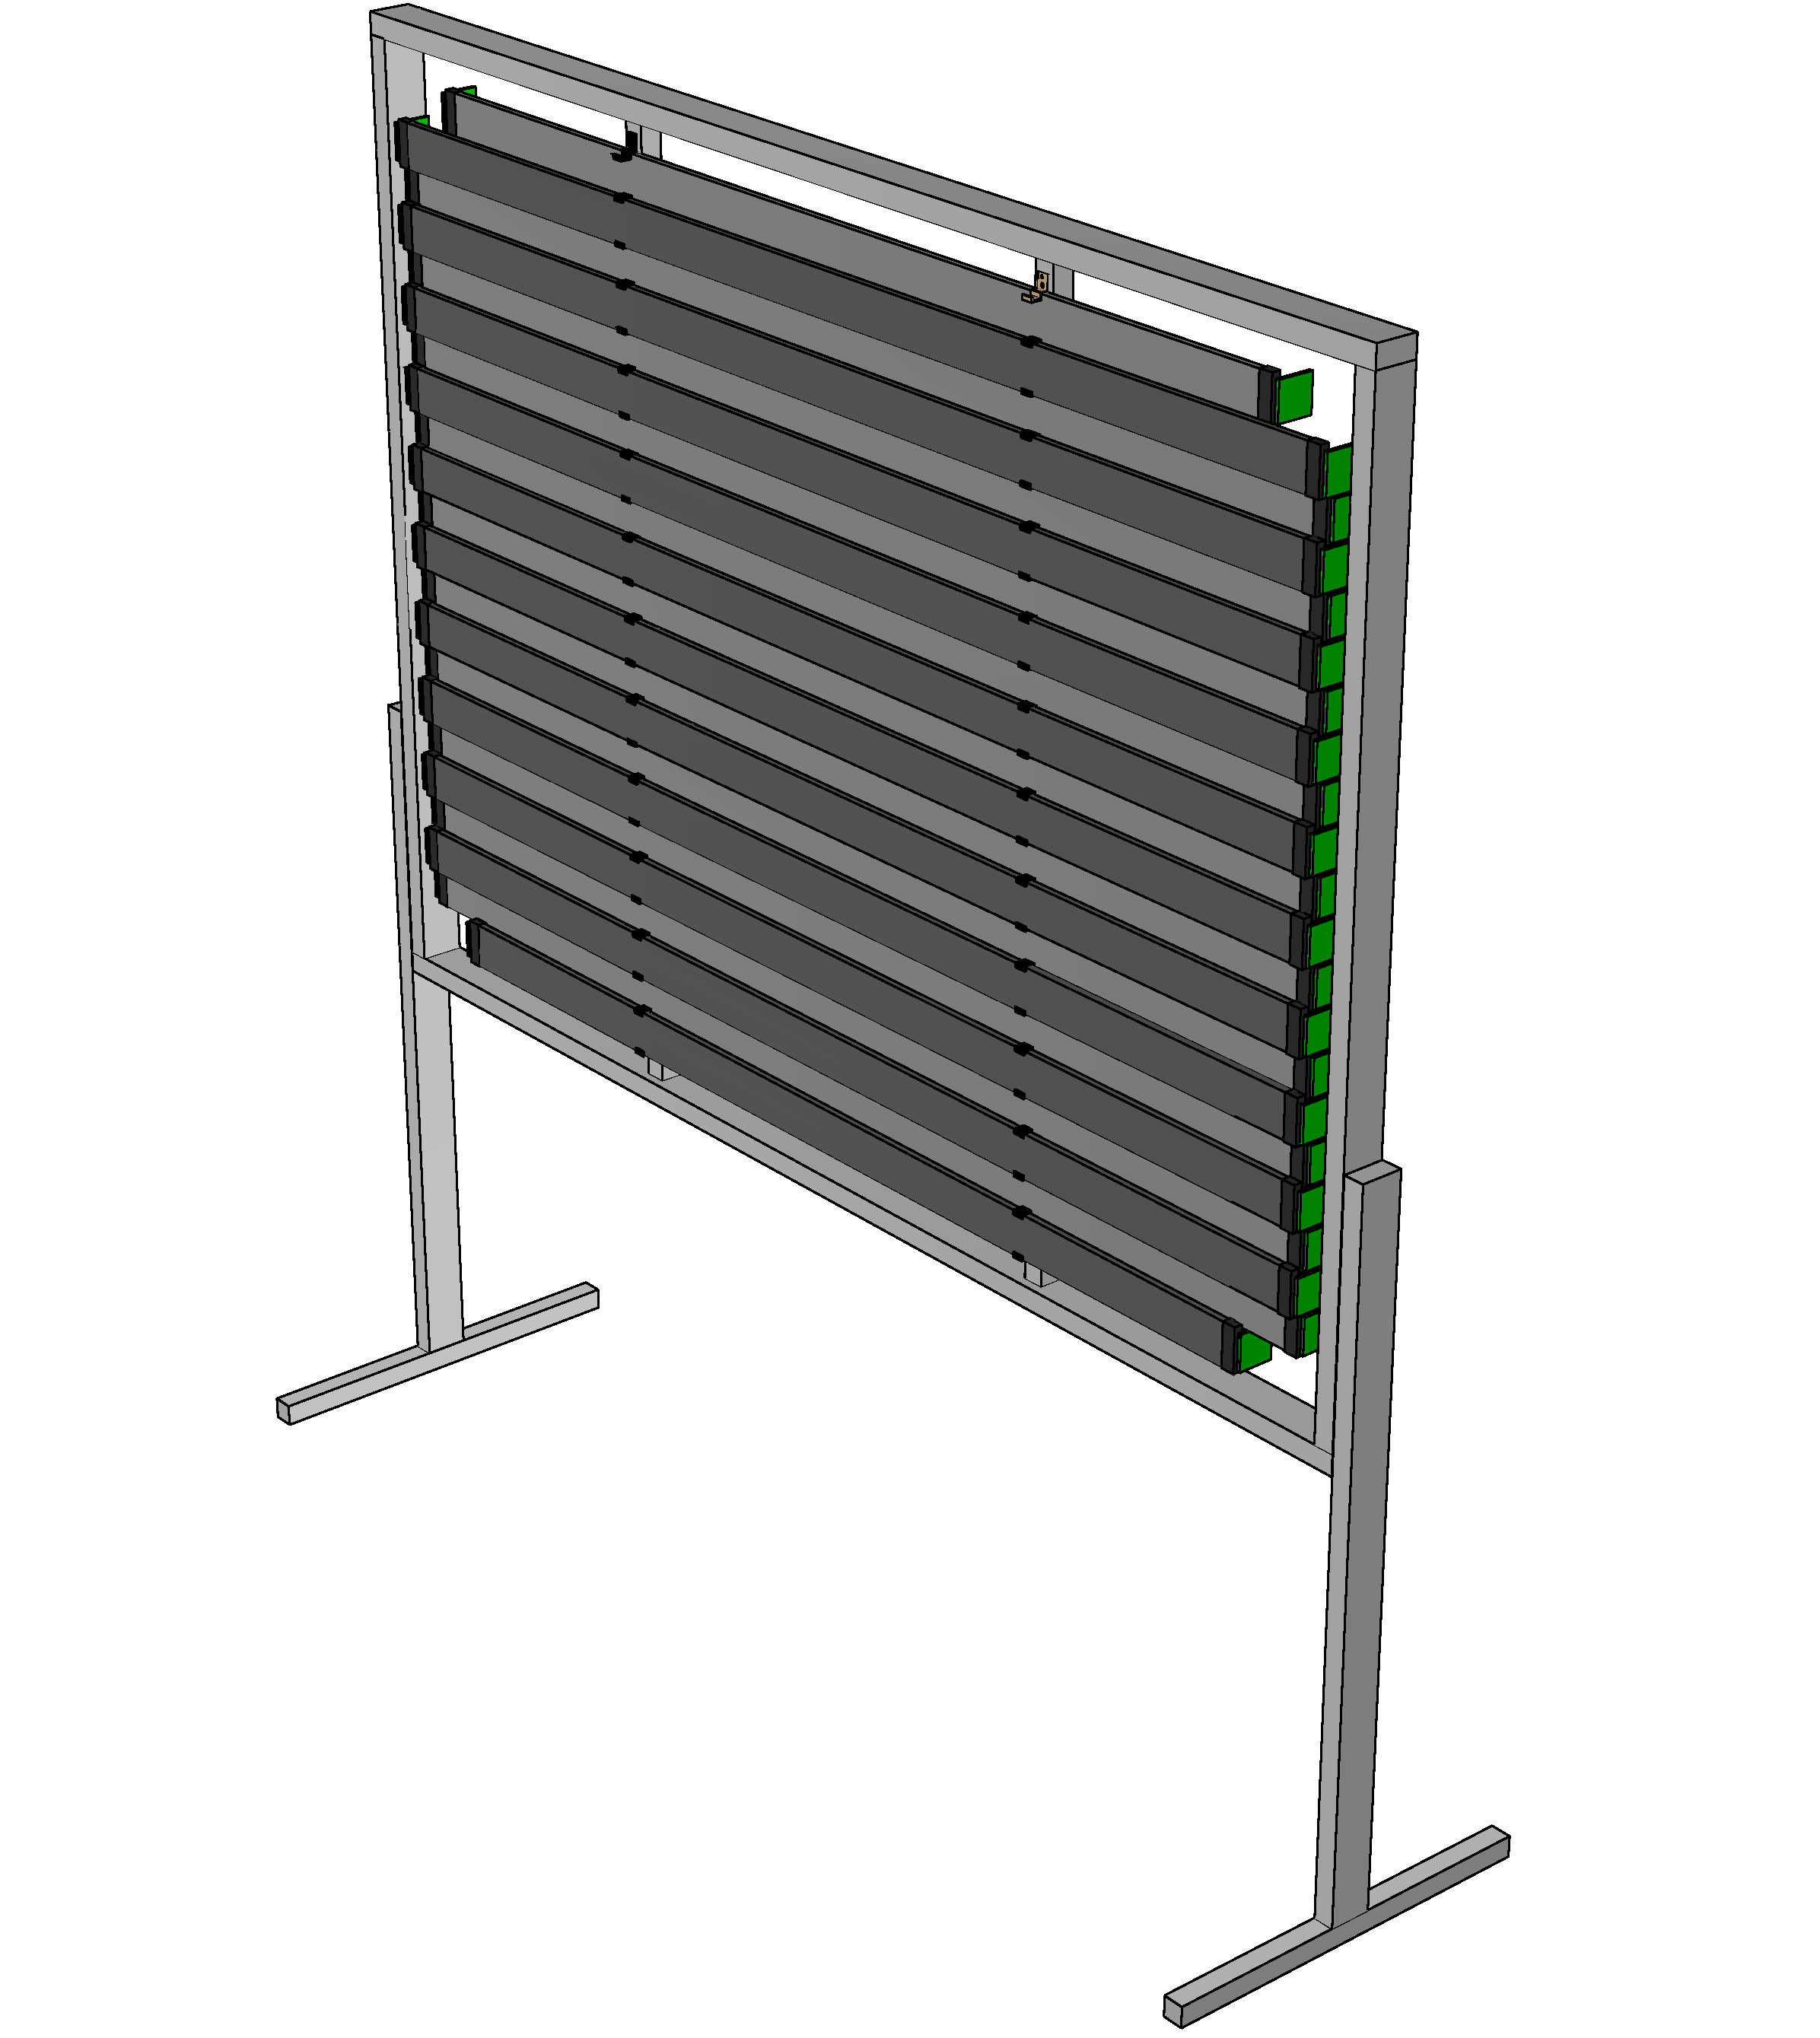
\includegraphics[width=\linewidth]{files/figures/hptpc_beam_flux/uTOF_rot}
  \end{minipage}
  \caption[Schematic diagrams of \SThree]{Front-on and rotated schematic diagrams of \SThree from~\cite{s3Paper} along with dimensions.}
  \label{fig:s3Diag}
\end{figure}

EJ-200 plastic scintillator (of which the bars are made) has a brightness of \num{10000}~photons/MeV deposited.
Additionally, it has a large optical attenuation length (\SI{4}{\metre}) along with a fast rise time and decay time constant (\SI{0.9}{\nano\second} and \SI{2.1}{\nano\second} respectively.
The scintillation emission spectrum peaks at a wavelength of \SI{435}{\nano\metre}~\cite{ej200}.
In order to increase the light collection capabilities of the bars while excluding background light, they are wrapped in aluminium foil which has a reflectivity of 60\%.

The scintillation photons produced by the bars are detected by S13360-6050PE Hamamatsu Photonics~\cite{hamamatsu} silicon photomultipliers (SiPMs) arranged at either end of the bar.
These photosensors, each measuring \SI{6 x 6}{\milli\metre}, are arranged in groups of eight and then coupled to the end of the bar.
These photomultipliers have a wavelength range that is well suited to the scintillation light produced by the bars (the sensitivity of the SiPMs at a wavelength of \SI{450}{\nano\metre} is 40\%~\cite{hamamatsu}).
The anode signals produced by these SiPMs are read out, summed and shaped by a dedicated circuit as described in~\cite{s3SiPM}.

These signals, along with those from \SOne and \STwo, are then fed into a DAQ based upon the SAMPIC chip, further details of which are given in~\cite{sampic}.

\SThree triggers are formed in the following manner, shown graphically in \citefig{fig:s3Trigger}, and are intended to identify the prescence of a beam particle travelling between \SOne and \SThree.
An \SOne signal is considered to have occurred when at least three of the four \SOne PMTs register a signal above the threshold of \SI{30}{\milli\volt}.
An \SThree signal is deemed to have occurred if the SiPMs on either end of a given bar register a signal above a threshold of \SI{30}{\milli\volt}.
If an \SOne signal and an \SThree signal occur within a time window of \SI{70}{\nano\second}, the DAQ is triggered and writes the event.
The DAQ also acquires signals from the coincidence of \SOne and \STwo as well as the signal indicating the start of the beam spill.

\begin{figure}[h]
  \centering
  \includegraphics[width=.8\linewidth]{files/figures/hptpc_beam_flux/utofTrig}
  \caption[Trigger logic for the upstream time of flight DAQ]{Trigger logic showing the necessary conditions for the identification of a $\SOne-\SThree$ beam particle by the upstream ToF DAQ.}
  \label{fig:s3Trigger}
\end{figure}


\subsection{The downstream time of flight detector (\SFour)}
\label{sec:hptpc_beam_flux:overview:s4}

The design of \SFour is primarily discussed in \citesec{sec:hptpc_dtof_characterisation:dtof}, however it will be briefly revisited here.
\SFour consists of 10 scintillator bars which together form an active area of \SI{1.40 x 0.78}{\metre}.
A diagram of one such bar is shown in \citefig{fig:barDiag}.
Each of these scintillator bars has a PMT attached to each end and these observe the scintillation light produced by charged particles traversing the bars.
A diagram of \SFour is shown in \citefig{fig:dtofDiag}.

The anode signal of each of the PMTs is fed into a LeCroy 620AL NIM discriminator with a threshold of \SI{-20}{\milli\volt}.
Any PMT signals above this threshold are digitised using a time-to-digital converted (TDC)
Additionally, the signal indicating the start of a beam spill as well as a signal indicating a coincidence between \SOne and \STwo were fed into the TDC.
A particle (either beam induced or otherwise) is considered to have been observed in \SFour if a signal above the discriminator threshold is recorded in both PMTs on the same bar, within \SI{20}{\nano\second} of each other.

Unlike the UToF DAQ system, the DToF DAQ is operated in self-triggering mode and thus acquired data both inside and outside the beam spill.


\section{Methods}
\label{sec:hptpc_beam_flux:methods}

In a beamline such as the T10 beamline at CERN, charged particles are selected using by momentum using a magnetic field.
This results in a beam of particles that are all of the same momentum but of different species.
Different particles of the same momentum will take different times to cover the same distance.
The time of flight, $t$, of a particle of mass, $m$, with a momentum, $p$, is given by
\begin{equation}
t = L \sqrt{ \frac{1}{c^{2}} + \frac{m^{2}}{p^{2}} }\, ,
\end{equation}
where $L$ is the distance travelled by the particle.
\citefig{fig:tofVsMom}, left and right, show the time of flight for various particles as a function of particle momentum for the $\SOne - \SThree$ and  $\STwo - \SFour$ distances respectively.
If the beam momentum is known, by measuring a particle's time of flight it should be possible to identify the particle in question.
One can see that, assuming a time resolution of around \SI{1}{\nano\second}, it should be possible to distinguish between deuterons, protons and pions/muons at the momenta used in this study.

\begin{figure}[h]
  \begin{minipage}[t]{.5\linewidth}
    \begin{adjustbox}{max totalsize=\textwidth, center}
      \begin{tikzpicture}
\pgfdeclareplotmark{cross} {
\pgfpathmoveto{\pgfpoint{-0.3\pgfplotmarksize}{\pgfplotmarksize}}
\pgfpathlineto{\pgfpoint{+0.3\pgfplotmarksize}{\pgfplotmarksize}}
\pgfpathlineto{\pgfpoint{+0.3\pgfplotmarksize}{0.3\pgfplotmarksize}}
\pgfpathlineto{\pgfpoint{+1\pgfplotmarksize}{0.3\pgfplotmarksize}}
\pgfpathlineto{\pgfpoint{+1\pgfplotmarksize}{-0.3\pgfplotmarksize}}
\pgfpathlineto{\pgfpoint{+0.3\pgfplotmarksize}{-0.3\pgfplotmarksize}}
\pgfpathlineto{\pgfpoint{+0.3\pgfplotmarksize}{-1.\pgfplotmarksize}}
\pgfpathlineto{\pgfpoint{-0.3\pgfplotmarksize}{-1.\pgfplotmarksize}}
\pgfpathlineto{\pgfpoint{-0.3\pgfplotmarksize}{-0.3\pgfplotmarksize}}
\pgfpathlineto{\pgfpoint{-1.\pgfplotmarksize}{-0.3\pgfplotmarksize}}
\pgfpathlineto{\pgfpoint{-1.\pgfplotmarksize}{0.3\pgfplotmarksize}}
\pgfpathlineto{\pgfpoint{-0.3\pgfplotmarksize}{0.3\pgfplotmarksize}}
\pgfpathclose
\pgfusepathqstroke
}
\pgfdeclareplotmark{cross*} {
\pgfpathmoveto{\pgfpoint{-0.3\pgfplotmarksize}{\pgfplotmarksize}}
\pgfpathlineto{\pgfpoint{+0.3\pgfplotmarksize}{\pgfplotmarksize}}
\pgfpathlineto{\pgfpoint{+0.3\pgfplotmarksize}{0.3\pgfplotmarksize}}
\pgfpathlineto{\pgfpoint{+1\pgfplotmarksize}{0.3\pgfplotmarksize}}
\pgfpathlineto{\pgfpoint{+1\pgfplotmarksize}{-0.3\pgfplotmarksize}}
\pgfpathlineto{\pgfpoint{+0.3\pgfplotmarksize}{-0.3\pgfplotmarksize}}
\pgfpathlineto{\pgfpoint{+0.3\pgfplotmarksize}{-1.\pgfplotmarksize}}
\pgfpathlineto{\pgfpoint{-0.3\pgfplotmarksize}{-1.\pgfplotmarksize}}
\pgfpathlineto{\pgfpoint{-0.3\pgfplotmarksize}{-0.3\pgfplotmarksize}}
\pgfpathlineto{\pgfpoint{-1.\pgfplotmarksize}{-0.3\pgfplotmarksize}}
\pgfpathlineto{\pgfpoint{-1.\pgfplotmarksize}{0.3\pgfplotmarksize}}
\pgfpathlineto{\pgfpoint{-0.3\pgfplotmarksize}{0.3\pgfplotmarksize}}
\pgfpathclose
\pgfusepathqfillstroke
}
\pgfdeclareplotmark{newstar} {
\pgfpathmoveto{\pgfqpoint{0pt}{\pgfplotmarksize}}
\pgfpathlineto{\pgfqpointpolar{44}{0.5\pgfplotmarksize}}
\pgfpathlineto{\pgfqpointpolar{18}{\pgfplotmarksize}}
\pgfpathlineto{\pgfqpointpolar{-20}{0.5\pgfplotmarksize}}
\pgfpathlineto{\pgfqpointpolar{-54}{\pgfplotmarksize}}
\pgfpathlineto{\pgfqpointpolar{-90}{0.5\pgfplotmarksize}}
\pgfpathlineto{\pgfqpointpolar{234}{\pgfplotmarksize}}
\pgfpathlineto{\pgfqpointpolar{198}{0.5\pgfplotmarksize}}
\pgfpathlineto{\pgfqpointpolar{162}{\pgfplotmarksize}}
\pgfpathlineto{\pgfqpointpolar{134}{0.5\pgfplotmarksize}}
\pgfpathclose
\pgfusepathqstroke
}
\pgfdeclareplotmark{newstar*} {
\pgfpathmoveto{\pgfqpoint{0pt}{\pgfplotmarksize}}
\pgfpathlineto{\pgfqpointpolar{44}{0.5\pgfplotmarksize}}
\pgfpathlineto{\pgfqpointpolar{18}{\pgfplotmarksize}}
\pgfpathlineto{\pgfqpointpolar{-20}{0.5\pgfplotmarksize}}
\pgfpathlineto{\pgfqpointpolar{-54}{\pgfplotmarksize}}
\pgfpathlineto{\pgfqpointpolar{-90}{0.5\pgfplotmarksize}}
\pgfpathlineto{\pgfqpointpolar{234}{\pgfplotmarksize}}
\pgfpathlineto{\pgfqpointpolar{198}{0.5\pgfplotmarksize}}
\pgfpathlineto{\pgfqpointpolar{162}{\pgfplotmarksize}}
\pgfpathlineto{\pgfqpointpolar{134}{0.5\pgfplotmarksize}}
\pgfpathclose
\pgfusepathqfillstroke
}
\definecolor{c}{rgb}{1,1,1};
\draw [color=c, fill=c] (0,0) rectangle (20,13.639);
\draw [color=c, fill=c] (2.60745,1.76218) rectangle (17.0201,11.8768);
\definecolor{c}{rgb}{0,0,0};
\draw [c,line width=0.9] (2.60745,1.76218) -- (2.60745,11.8768) -- (17.0201,11.8768) -- (17.0201,1.76218) -- (2.60745,1.76218);
\definecolor{c}{rgb}{1,1,1};
\draw [color=c, fill=c] (2.60745,1.76218) rectangle (17.0201,11.8768);
\definecolor{c}{rgb}{0,0,0};
\draw [c,line width=0.9] (2.60745,1.76218) -- (2.60745,11.8768) -- (17.0201,11.8768) -- (17.0201,1.76218) -- (2.60745,1.76218);
\definecolor{c}{rgb}{0,0.8,0.8};
\draw [c,line width=1.8] (2.67951,3.58458) -- (2.82364,3.40401) -- (2.96777,3.25475) -- (3.11189,3.12999) -- (3.25602,3.02465) -- (3.40014,2.93493) -- (3.54427,2.85792) -- (3.6884,2.79135) -- (3.83252,2.73344) -- (3.97665,2.68276) --
 (4.12077,2.63817) -- (4.2649,2.59875) -- (4.40903,2.56374) -- (4.55315,2.53252) -- (4.69728,2.50455) -- (4.8414,2.47942) -- (4.98553,2.45675) -- (5.12966,2.43624) -- (5.27378,2.41763) -- (5.41791,2.40068) -- (5.56203,2.38522) -- (5.70616,2.37107) --
 (5.85029,2.35809) -- (5.99441,2.34616) -- (6.13854,2.33516) -- (6.28266,2.32501) -- (6.42679,2.31562) -- (6.57092,2.30691) -- (6.71504,2.29883) -- (6.85917,2.29131) -- (7.0033,2.2843) -- (7.14742,2.27777) -- (7.29155,2.27166) -- (7.43567,2.26594) --
 (7.5798,2.26058) -- (7.72393,2.25555) -- (7.86805,2.25083) -- (8.01218,2.24638) -- (8.1563,2.24219) -- (8.30043,2.23824) -- (8.44456,2.23451) -- (8.58868,2.23099) -- (8.73281,2.22766) -- (8.87693,2.2245) -- (9.02106,2.22151) -- (9.16519,2.21867) --
 (9.30931,2.21598) -- (9.45344,2.21342) -- (9.59756,2.21098) -- (9.74169,2.20866);
\draw [c,line width=1.8] (9.74169,2.20866) -- (9.88582,2.20645) -- (10.0299,2.20435) -- (10.1741,2.20234) -- (10.3182,2.20042) -- (10.4623,2.19858) -- (10.6064,2.19683) -- (10.7506,2.19516) -- (10.8947,2.19355) -- (11.0388,2.19201) --
 (11.183,2.19054) -- (11.3271,2.18913) -- (11.4712,2.18777) -- (11.6153,2.18647) -- (11.7595,2.18522) -- (11.9036,2.18401) -- (12.0477,2.18286) -- (12.1918,2.18175) -- (12.336,2.18068) -- (12.4801,2.17965) -- (12.6242,2.17865) -- (12.7683,2.17769) --
 (12.9125,2.17677) -- (13.0566,2.17588) -- (13.2007,2.17502) -- (13.3448,2.17419) -- (13.489,2.17339) -- (13.6331,2.17261) -- (13.7772,2.17187) -- (13.9213,2.17114) -- (14.0655,2.17044) -- (14.2096,2.16976) -- (14.3537,2.16911) -- (14.4979,2.16847)
 -- (14.642,2.16786) -- (14.7861,2.16726) -- (14.9302,2.16668) -- (15.0744,2.16612) -- (15.2185,2.16558) -- (15.3626,2.16505) -- (15.5067,2.16454) -- (15.6509,2.16404) -- (15.795,2.16356) -- (15.9391,2.16309) -- (16.0832,2.16263) -- (16.2274,2.16219)
 -- (16.3715,2.16176) -- (16.5156,2.16134) -- (16.6597,2.16093) -- (16.8039,2.16053);
\draw [c,line width=1.8] (16.8039,2.16053) -- (16.948,2.16015);
\definecolor{c}{rgb}{0,0,0};
\draw [c,line width=0.9] (2.60745,1.76218) -- (17.0201,1.76218);
\draw [c,line width=0.9] (2.60745,2.05704) -- (2.60745,1.76218);
\draw [c,line width=0.9] (2.92773,1.90961) -- (2.92773,1.76218);
\draw [c,line width=0.9] (3.24801,1.90961) -- (3.24801,1.76218);
\draw [c,line width=0.9] (3.56829,1.90961) -- (3.56829,1.76218);
\draw [c,line width=0.9] (3.88857,1.90961) -- (3.88857,1.76218);
\draw [c,line width=0.9] (4.20885,2.05704) -- (4.20885,1.76218);
\draw [c,line width=0.9] (4.52913,1.90961) -- (4.52913,1.76218);
\draw [c,line width=0.9] (4.84941,1.90961) -- (4.84941,1.76218);
\draw [c,line width=0.9] (5.16969,1.90961) -- (5.16969,1.76218);
\draw [c,line width=0.9] (5.48997,1.90961) -- (5.48997,1.76218);
\draw [c,line width=0.9] (5.81025,2.05704) -- (5.81025,1.76218);
\draw [c,line width=0.9] (6.13053,1.90961) -- (6.13053,1.76218);
\draw [c,line width=0.9] (6.45081,1.90961) -- (6.45081,1.76218);
\draw [c,line width=0.9] (6.77109,1.90961) -- (6.77109,1.76218);
\draw [c,line width=0.9] (7.09137,1.90961) -- (7.09137,1.76218);
\draw [c,line width=0.9] (7.41165,2.05704) -- (7.41165,1.76218);
\draw [c,line width=0.9] (7.73193,1.90961) -- (7.73193,1.76218);
\draw [c,line width=0.9] (8.05221,1.90961) -- (8.05221,1.76218);
\draw [c,line width=0.9] (8.37249,1.90961) -- (8.37249,1.76218);
\draw [c,line width=0.9] (8.69277,1.90961) -- (8.69277,1.76218);
\draw [c,line width=0.9] (9.01305,2.05704) -- (9.01305,1.76218);
\draw [c,line width=0.9] (9.33333,1.90961) -- (9.33333,1.76218);
\draw [c,line width=0.9] (9.65361,1.90961) -- (9.65361,1.76218);
\draw [c,line width=0.9] (9.97389,1.90961) -- (9.97389,1.76218);
\draw [c,line width=0.9] (10.2942,1.90961) -- (10.2942,1.76218);
\draw [c,line width=0.9] (10.6145,2.05704) -- (10.6145,1.76218);
\draw [c,line width=0.9] (10.9347,1.90961) -- (10.9347,1.76218);
\draw [c,line width=0.9] (11.255,1.90961) -- (11.255,1.76218);
\draw [c,line width=0.9] (11.5753,1.90961) -- (11.5753,1.76218);
\draw [c,line width=0.9] (11.8956,1.90961) -- (11.8956,1.76218);
\draw [c,line width=0.9] (12.2159,2.05704) -- (12.2159,1.76218);
\draw [c,line width=0.9] (12.5361,1.90961) -- (12.5361,1.76218);
\draw [c,line width=0.9] (12.8564,1.90961) -- (12.8564,1.76218);
\draw [c,line width=0.9] (13.1767,1.90961) -- (13.1767,1.76218);
\draw [c,line width=0.9] (13.497,1.90961) -- (13.497,1.76218);
\draw [c,line width=0.9] (13.8173,2.05704) -- (13.8173,1.76218);
\draw [c,line width=0.9] (14.1375,1.90961) -- (14.1375,1.76218);
\draw [c,line width=0.9] (14.4578,1.90961) -- (14.4578,1.76218);
\draw [c,line width=0.9] (14.7781,1.90961) -- (14.7781,1.76218);
\draw [c,line width=0.9] (15.0984,1.90961) -- (15.0984,1.76218);
\draw [c,line width=0.9] (15.4187,2.05704) -- (15.4187,1.76218);
\draw [c,line width=0.9] (15.7389,1.90961) -- (15.7389,1.76218);
\draw [c,line width=0.9] (16.0592,1.90961) -- (16.0592,1.76218);
\draw [c,line width=0.9] (16.3795,1.90961) -- (16.3795,1.76218);
\draw [c,line width=0.9] (16.6998,1.90961) -- (16.6998,1.76218);
\draw [c,line width=0.9] (17.0201,2.05704) -- (17.0201,1.76218);
\draw [anchor=base] (2.60745,1.14842) node[scale=1.52731, color=c, rotate=0]{0.1};
\draw [anchor=base] (4.20885,1.14842) node[scale=1.52731, color=c, rotate=0]{0.2};
\draw [anchor=base] (5.81025,1.14842) node[scale=1.52731, color=c, rotate=0]{0.3};
\draw [anchor=base] (7.41165,1.14842) node[scale=1.52731, color=c, rotate=0]{0.4};
\draw [anchor=base] (9.01305,1.14842) node[scale=1.52731, color=c, rotate=0]{0.5};
\draw [anchor=base] (10.6145,1.14842) node[scale=1.52731, color=c, rotate=0]{0.6};
\draw [anchor=base] (12.2159,1.14842) node[scale=1.52731, color=c, rotate=0]{0.7};
\draw [anchor=base] (13.8173,1.14842) node[scale=1.52731, color=c, rotate=0]{0.8};
\draw [anchor=base] (15.4187,1.14842) node[scale=1.52731, color=c, rotate=0]{0.9};
\draw [anchor=base] (17.0201,1.14842) node[scale=1.52731, color=c, rotate=0]{1};
\draw [anchor= east] (17.0201,0.561948) node[scale=1.52731, color=c, rotate=0]{ Particle momentum [\si{\giga\electronvolt\per\clight}]};
\draw [c,line width=0.9] (2.60745,11.8768) -- (17.0201,11.8768);
\draw [c,line width=0.9] (2.60745,11.5819) -- (2.60745,11.8768);
\draw [c,line width=0.9] (2.92773,11.7294) -- (2.92773,11.8768);
\draw [c,line width=0.9] (3.24801,11.7294) -- (3.24801,11.8768);
\draw [c,line width=0.9] (3.56829,11.7294) -- (3.56829,11.8768);
\draw [c,line width=0.9] (3.88857,11.7294) -- (3.88857,11.8768);
\draw [c,line width=0.9] (4.20885,11.5819) -- (4.20885,11.8768);
\draw [c,line width=0.9] (4.52913,11.7294) -- (4.52913,11.8768);
\draw [c,line width=0.9] (4.84941,11.7294) -- (4.84941,11.8768);
\draw [c,line width=0.9] (5.16969,11.7294) -- (5.16969,11.8768);
\draw [c,line width=0.9] (5.48997,11.7294) -- (5.48997,11.8768);
\draw [c,line width=0.9] (5.81025,11.5819) -- (5.81025,11.8768);
\draw [c,line width=0.9] (6.13053,11.7294) -- (6.13053,11.8768);
\draw [c,line width=0.9] (6.45081,11.7294) -- (6.45081,11.8768);
\draw [c,line width=0.9] (6.77109,11.7294) -- (6.77109,11.8768);
\draw [c,line width=0.9] (7.09137,11.7294) -- (7.09137,11.8768);
\draw [c,line width=0.9] (7.41165,11.5819) -- (7.41165,11.8768);
\draw [c,line width=0.9] (7.73193,11.7294) -- (7.73193,11.8768);
\draw [c,line width=0.9] (8.05221,11.7294) -- (8.05221,11.8768);
\draw [c,line width=0.9] (8.37249,11.7294) -- (8.37249,11.8768);
\draw [c,line width=0.9] (8.69277,11.7294) -- (8.69277,11.8768);
\draw [c,line width=0.9] (9.01305,11.5819) -- (9.01305,11.8768);
\draw [c,line width=0.9] (9.33333,11.7294) -- (9.33333,11.8768);
\draw [c,line width=0.9] (9.65361,11.7294) -- (9.65361,11.8768);
\draw [c,line width=0.9] (9.97389,11.7294) -- (9.97389,11.8768);
\draw [c,line width=0.9] (10.2942,11.7294) -- (10.2942,11.8768);
\draw [c,line width=0.9] (10.6145,11.5819) -- (10.6145,11.8768);
\draw [c,line width=0.9] (10.9347,11.7294) -- (10.9347,11.8768);
\draw [c,line width=0.9] (11.255,11.7294) -- (11.255,11.8768);
\draw [c,line width=0.9] (11.5753,11.7294) -- (11.5753,11.8768);
\draw [c,line width=0.9] (11.8956,11.7294) -- (11.8956,11.8768);
\draw [c,line width=0.9] (12.2159,11.5819) -- (12.2159,11.8768);
\draw [c,line width=0.9] (12.5361,11.7294) -- (12.5361,11.8768);
\draw [c,line width=0.9] (12.8564,11.7294) -- (12.8564,11.8768);
\draw [c,line width=0.9] (13.1767,11.7294) -- (13.1767,11.8768);
\draw [c,line width=0.9] (13.497,11.7294) -- (13.497,11.8768);
\draw [c,line width=0.9] (13.8173,11.5819) -- (13.8173,11.8768);
\draw [c,line width=0.9] (14.1375,11.7294) -- (14.1375,11.8768);
\draw [c,line width=0.9] (14.4578,11.7294) -- (14.4578,11.8768);
\draw [c,line width=0.9] (14.7781,11.7294) -- (14.7781,11.8768);
\draw [c,line width=0.9] (15.0984,11.7294) -- (15.0984,11.8768);
\draw [c,line width=0.9] (15.4187,11.5819) -- (15.4187,11.8768);
\draw [c,line width=0.9] (15.7389,11.7294) -- (15.7389,11.8768);
\draw [c,line width=0.9] (16.0592,11.7294) -- (16.0592,11.8768);
\draw [c,line width=0.9] (16.3795,11.7294) -- (16.3795,11.8768);
\draw [c,line width=0.9] (16.6998,11.7294) -- (16.6998,11.8768);
\draw [c,line width=0.9] (17.0201,11.5819) -- (17.0201,11.8768);
\draw [c,line width=0.9] (2.60745,1.76218) -- (2.60745,11.8768);
\draw [c,line width=0.9] (3.05241,2.35715) -- (2.60745,2.35715);
\draw [c,line width=0.9] (2.82993,2.65464) -- (2.60745,2.65464);
\draw [c,line width=0.9] (2.82993,2.95213) -- (2.60745,2.95213);
\draw [c,line width=0.9] (2.82993,3.24962) -- (2.60745,3.24962);
\draw [c,line width=0.9] (3.05241,3.54711) -- (2.60745,3.54711);
\draw [c,line width=0.9] (2.82993,3.8446) -- (2.60745,3.8446);
\draw [c,line width=0.9] (2.82993,4.14209) -- (2.60745,4.14209);
\draw [c,line width=0.9] (2.82993,4.43958) -- (2.60745,4.43958);
\draw [c,line width=0.9] (3.05241,4.73706) -- (2.60745,4.73706);
\draw [c,line width=0.9] (2.82993,5.03455) -- (2.60745,5.03455);
\draw [c,line width=0.9] (2.82993,5.33204) -- (2.60745,5.33204);
\draw [c,line width=0.9] (2.82993,5.62953) -- (2.60745,5.62953);
\draw [c,line width=0.9] (3.05241,5.92702) -- (2.60745,5.92702);
\draw [c,line width=0.9] (2.82993,6.22451) -- (2.60745,6.22451);
\draw [c,line width=0.9] (2.82993,6.522) -- (2.60745,6.522);
\draw [c,line width=0.9] (2.82993,6.81948) -- (2.60745,6.81948);
\draw [c,line width=0.9] (3.05241,7.11697) -- (2.60745,7.11697);
\draw [c,line width=0.9] (2.82993,7.41446) -- (2.60745,7.41446);
\draw [c,line width=0.9] (2.82993,7.71195) -- (2.60745,7.71195);
\draw [c,line width=0.9] (2.82993,8.00944) -- (2.60745,8.00944);
\draw [c,line width=0.9] (3.05241,8.30693) -- (2.60745,8.30693);
\draw [c,line width=0.9] (2.82993,8.60442) -- (2.60745,8.60442);
\draw [c,line width=0.9] (2.82993,8.90191) -- (2.60745,8.90191);
\draw [c,line width=0.9] (2.82993,9.19939) -- (2.60745,9.19939);
\draw [c,line width=0.9] (3.05241,9.49688) -- (2.60745,9.49688);
\draw [c,line width=0.9] (2.82993,9.79437) -- (2.60745,9.79437);
\draw [c,line width=0.9] (2.82993,10.0919) -- (2.60745,10.0919);
\draw [c,line width=0.9] (2.82993,10.3893) -- (2.60745,10.3893);
\draw [c,line width=0.9] (3.05241,10.6868) -- (2.60745,10.6868);
\draw [c,line width=0.9] (2.82993,10.9843) -- (2.60745,10.9843);
\draw [c,line width=0.9] (2.82993,11.2818) -- (2.60745,11.2818);
\draw [c,line width=0.9] (2.82993,11.5793) -- (2.60745,11.5793);
\draw [c,line width=0.9] (3.05241,11.8768) -- (2.60745,11.8768);
\draw [c,line width=0.9] (3.05241,2.35715) -- (2.60745,2.35715);
\draw [c,line width=0.9] (2.82993,2.05967) -- (2.60745,2.05967);
\draw [c,line width=0.9] (2.82993,1.76218) -- (2.60745,1.76218);
\draw [anchor= east] (2.50745,2.35715) node[scale=1.52731, color=c, rotate=0]{40};
\draw [anchor= east] (2.50745,3.54711) node[scale=1.52731, color=c, rotate=0]{60};
\draw [anchor= east] (2.50745,4.73706) node[scale=1.52731, color=c, rotate=0]{80};
\draw [anchor= east] (2.50745,5.92702) node[scale=1.52731, color=c, rotate=0]{100};
\draw [anchor= east] (2.50745,7.11697) node[scale=1.52731, color=c, rotate=0]{120};
\draw [anchor= east] (2.50745,8.30693) node[scale=1.52731, color=c, rotate=0]{140};
\draw [anchor= east] (2.50745,9.49688) node[scale=1.52731, color=c, rotate=0]{160};
\draw [anchor= east] (2.50745,10.6868) node[scale=1.52731, color=c, rotate=0]{180};
\draw [anchor= east] (2.50745,11.8768) node[scale=1.52731, color=c, rotate=0]{200};
\draw [anchor= east] (0.84745,11.8768) node[scale=1.52731, color=c, rotate=90]{ Time of flight [\si{\nano\second}]};
\draw [c,line width=0.9] (17.0201,1.76218) -- (17.0201,11.8768);
\draw [c,line width=0.9] (16.5751,2.35715) -- (17.0201,2.35715);
\draw [c,line width=0.9] (16.7976,2.65464) -- (17.0201,2.65464);
\draw [c,line width=0.9] (16.7976,2.95213) -- (17.0201,2.95213);
\draw [c,line width=0.9] (16.7976,3.24962) -- (17.0201,3.24962);
\draw [c,line width=0.9] (16.5751,3.54711) -- (17.0201,3.54711);
\draw [c,line width=0.9] (16.7976,3.8446) -- (17.0201,3.8446);
\draw [c,line width=0.9] (16.7976,4.14209) -- (17.0201,4.14209);
\draw [c,line width=0.9] (16.7976,4.43958) -- (17.0201,4.43958);
\draw [c,line width=0.9] (16.5751,4.73706) -- (17.0201,4.73706);
\draw [c,line width=0.9] (16.7976,5.03455) -- (17.0201,5.03455);
\draw [c,line width=0.9] (16.7976,5.33204) -- (17.0201,5.33204);
\draw [c,line width=0.9] (16.7976,5.62953) -- (17.0201,5.62953);
\draw [c,line width=0.9] (16.5751,5.92702) -- (17.0201,5.92702);
\draw [c,line width=0.9] (16.7976,6.22451) -- (17.0201,6.22451);
\draw [c,line width=0.9] (16.7976,6.522) -- (17.0201,6.522);
\draw [c,line width=0.9] (16.7976,6.81948) -- (17.0201,6.81948);
\draw [c,line width=0.9] (16.5751,7.11697) -- (17.0201,7.11697);
\draw [c,line width=0.9] (16.7976,7.41446) -- (17.0201,7.41446);
\draw [c,line width=0.9] (16.7976,7.71195) -- (17.0201,7.71195);
\draw [c,line width=0.9] (16.7976,8.00944) -- (17.0201,8.00944);
\draw [c,line width=0.9] (16.5751,8.30693) -- (17.0201,8.30693);
\draw [c,line width=0.9] (16.7976,8.60442) -- (17.0201,8.60442);
\draw [c,line width=0.9] (16.7976,8.90191) -- (17.0201,8.90191);
\draw [c,line width=0.9] (16.7976,9.19939) -- (17.0201,9.19939);
\draw [c,line width=0.9] (16.5751,9.49688) -- (17.0201,9.49688);
\draw [c,line width=0.9] (16.7976,9.79437) -- (17.0201,9.79437);
\draw [c,line width=0.9] (16.7976,10.0919) -- (17.0201,10.0919);
\draw [c,line width=0.9] (16.7976,10.3893) -- (17.0201,10.3893);
\draw [c,line width=0.9] (16.5751,10.6868) -- (17.0201,10.6868);
\draw [c,line width=0.9] (16.7976,10.9843) -- (17.0201,10.9843);
\draw [c,line width=0.9] (16.7976,11.2818) -- (17.0201,11.2818);
\draw [c,line width=0.9] (16.7976,11.5793) -- (17.0201,11.5793);
\draw [c,line width=0.9] (16.5751,11.8768) -- (17.0201,11.8768);
\draw [c,line width=0.9] (16.5751,2.35715) -- (17.0201,2.35715);
\draw [c,line width=0.9] (16.7976,2.05967) -- (17.0201,2.05967);
\draw [c,line width=0.9] (16.7976,1.76218) -- (17.0201,1.76218);
\definecolor{c}{rgb}{1,0,0};
\draw [c,line width=1.8] (3.78368,11.8768) -- (3.83252,11.671);
\draw [c,line width=1.8] (3.83252,11.671) -- (3.97665,11.1235) -- (4.12077,10.6276) -- (4.2649,10.1764) -- (4.40903,9.76425) -- (4.55315,9.38637) -- (4.69728,9.03875) -- (4.8414,8.71797) -- (4.98553,8.42111) -- (5.12966,8.14566) -- (5.27378,7.88943)
 -- (5.41791,7.65056) -- (5.56203,7.42737) -- (5.70616,7.21843) -- (5.85029,7.02246) -- (5.99441,6.83832) -- (6.13854,6.66503) -- (6.28266,6.50169) -- (6.42679,6.34749) -- (6.57092,6.20173) -- (6.71504,6.06376) -- (6.85917,5.933) -- (7.0033,5.80893)
 -- (7.14742,5.69107) -- (7.29155,5.57899) -- (7.43567,5.47231) -- (7.5798,5.37065) -- (7.72393,5.2737) -- (7.86805,5.18115) -- (8.01218,5.09273) -- (8.1563,5.00819) -- (8.30043,4.92729) -- (8.44456,4.84982) -- (8.58868,4.77557) -- (8.73281,4.70437)
 -- (8.87693,4.63605) -- (9.02106,4.57044) -- (9.16519,4.5074) -- (9.30931,4.4468) -- (9.45344,4.3885) -- (9.59756,4.33238) -- (9.74169,4.27834) -- (9.88582,4.22628) -- (10.0299,4.17608) -- (10.1741,4.12767) -- (10.3182,4.08096) -- (10.4623,4.03587)
 -- (10.6064,3.99232) -- (10.7506,3.95024);
\draw [c,line width=1.8] (10.7506,3.95024) -- (10.8947,3.90957) -- (11.0388,3.87024) -- (11.183,3.83219) -- (11.3271,3.79537) -- (11.4712,3.75972) -- (11.6153,3.72519) -- (11.7595,3.69175) -- (11.9036,3.65933) -- (12.0477,3.62791) --
 (12.1918,3.59744) -- (12.336,3.56787) -- (12.4801,3.53918) -- (12.6242,3.51134) -- (12.7683,3.4843) -- (12.9125,3.45804) -- (13.0566,3.43252) -- (13.2007,3.40773) -- (13.3448,3.38363) -- (13.489,3.36019) -- (13.6331,3.3374) -- (13.7772,3.31523) --
 (13.9213,3.29365) -- (14.0655,3.27265) -- (14.2096,3.25221) -- (14.3537,3.2323) -- (14.4979,3.21291) -- (14.642,3.19402) -- (14.7861,3.17561) -- (14.9302,3.15767) -- (15.0744,3.14019) -- (15.2185,3.12314) -- (15.3626,3.10651) -- (15.5067,3.09029) --
 (15.6509,3.07446) -- (15.795,3.05902) -- (15.9391,3.04395) -- (16.0832,3.02923) -- (16.2274,3.01487) -- (16.3715,3.00084) -- (16.5156,2.98714) -- (16.6597,2.97375) -- (16.8039,2.96067) -- (16.948,2.94789);
\definecolor{c}{rgb}{0,0,1};
\draw [c,line width=1.8] (2.67951,3.05203) -- (2.82364,2.93124) -- (2.96777,2.83249) -- (3.11189,2.75078) -- (3.25602,2.68244) -- (3.40014,2.62473) -- (3.54427,2.5756) -- (3.6884,2.53343) -- (3.83252,2.497) -- (3.97665,2.46531) -- (4.12077,2.43759)
 -- (4.2649,2.41321) -- (4.40903,2.39166) -- (4.55315,2.37252) -- (4.69728,2.35545) -- (4.8414,2.34017) -- (4.98553,2.32643) -- (5.12966,2.31404) -- (5.27378,2.30282) -- (5.41791,2.29264) -- (5.56203,2.28337) -- (5.70616,2.27491) -- (5.85029,2.26717)
 -- (5.99441,2.26006) -- (6.13854,2.25353) -- (6.28266,2.2475) -- (6.42679,2.24194) -- (6.57092,2.23679) -- (6.71504,2.23201) -- (6.85917,2.22758) -- (7.0033,2.22345) -- (7.14742,2.2196) -- (7.29155,2.21601) -- (7.43567,2.21265) -- (7.5798,2.20951)
 -- (7.72393,2.20656) -- (7.86805,2.20379) -- (8.01218,2.20119) -- (8.1563,2.19874) -- (8.30043,2.19644) -- (8.44456,2.19426) -- (8.58868,2.1922) -- (8.73281,2.19026) -- (8.87693,2.18842) -- (9.02106,2.18668) -- (9.16519,2.18503) -- (9.30931,2.18346)
 -- (9.45344,2.18197) -- (9.59756,2.18055) -- (9.74169,2.1792);
\draw [c,line width=1.8] (9.74169,2.1792) -- (9.88582,2.17792) -- (10.0299,2.1767) -- (10.1741,2.17553) -- (10.3182,2.17442) -- (10.4623,2.17336) -- (10.6064,2.17234) -- (10.7506,2.17137) -- (10.8947,2.17044) -- (11.0388,2.16955) -- (11.183,2.16869)
 -- (11.3271,2.16788) -- (11.4712,2.16709) -- (11.6153,2.16634) -- (11.7595,2.16561) -- (11.9036,2.16492) -- (12.0477,2.16425) -- (12.1918,2.16361) -- (12.336,2.16299) -- (12.4801,2.16239) -- (12.6242,2.16182) -- (12.7683,2.16127) --
 (12.9125,2.16073) -- (13.0566,2.16022) -- (13.2007,2.15972) -- (13.3448,2.15924) -- (13.489,2.15878) -- (13.6331,2.15833) -- (13.7772,2.1579) -- (13.9213,2.15748) -- (14.0655,2.15708) -- (14.2096,2.15669) -- (14.3537,2.15631) -- (14.4979,2.15594) --
 (14.642,2.15559) -- (14.7861,2.15524) -- (14.9302,2.15491) -- (15.0744,2.15459) -- (15.2185,2.15427) -- (15.3626,2.15397) -- (15.5067,2.15367) -- (15.6509,2.15339) -- (15.795,2.15311) -- (15.9391,2.15284) -- (16.0832,2.15258) -- (16.2274,2.15232) --
 (16.3715,2.15207) -- (16.5156,2.15183) -- (16.6597,2.1516) -- (16.8039,2.15137);
\draw [c,line width=1.8] (16.8039,2.15137) -- (16.948,2.15115);
\definecolor{c}{rgb}{1,0.6,0.2};
\draw [c,line width=1.8] (2.67951,10.4165) -- (2.82364,9.62568) -- (2.96777,8.95373) -- (3.11189,8.37623) -- (3.25602,7.87499) -- (3.40014,7.43621) -- (3.54427,7.04923) -- (3.6884,6.70565) -- (3.83252,6.39883) -- (3.97665,6.12337) -- (4.12077,5.8749)
 -- (4.2649,5.64981) -- (4.40903,5.44511) -- (4.55315,5.25828) -- (4.69728,5.08721) -- (4.8414,4.9301) -- (4.98553,4.78541) -- (5.12966,4.65181) -- (5.27378,4.52817) -- (5.41791,4.41348) -- (5.56203,4.30688) -- (5.70616,4.2076) -- (5.85029,4.11497)
 -- (5.99441,4.02841) -- (6.13854,3.94737) -- (6.28266,3.8714) -- (6.42679,3.80006) -- (6.57092,3.733) -- (6.71504,3.66987) -- (6.85917,3.61036) -- (7.0033,3.5542) -- (7.14742,3.50115) -- (7.29155,3.45098) -- (7.43567,3.40348) -- (7.5798,3.35846) --
 (7.72393,3.31576) -- (7.86805,3.27522) -- (8.01218,3.2367) -- (8.1563,3.20007) -- (8.30043,3.16519) -- (8.44456,3.13198) -- (8.58868,3.10031) -- (8.73281,3.07011) -- (8.87693,3.04127) -- (9.02106,3.01373) -- (9.16519,2.98739) -- (9.30931,2.96221) --
 (9.45344,2.9381) -- (9.59756,2.91501) -- (9.74169,2.89289);
\draw [c,line width=1.8] (9.74169,2.89289) -- (9.88582,2.87167) -- (10.0299,2.85132) -- (10.1741,2.83179) -- (10.3182,2.81303) -- (10.4623,2.79501) -- (10.6064,2.77768) -- (10.7506,2.76102) -- (10.8947,2.74498) -- (11.0388,2.72955) --
 (11.183,2.71468) -- (11.3271,2.70035) -- (11.4712,2.68655) -- (11.6153,2.67323) -- (11.7595,2.66038) -- (11.9036,2.64799) -- (12.0477,2.63602) -- (12.1918,2.62446) -- (12.336,2.61329) -- (12.4801,2.60249) -- (12.6242,2.59205) -- (12.7683,2.58195) --
 (12.9125,2.57218) -- (13.0566,2.56272) -- (13.2007,2.55356) -- (13.3448,2.5447) -- (13.489,2.5361) -- (13.6331,2.52778) -- (13.7772,2.5197) -- (13.9213,2.51187) -- (14.0655,2.50428) -- (14.2096,2.49691) -- (14.3537,2.48976) -- (14.4979,2.48282) --
 (14.642,2.47607) -- (14.7861,2.46952) -- (14.9302,2.46316) -- (15.0744,2.45697) -- (15.2185,2.45096) -- (15.3626,2.44512) -- (15.5067,2.43943) -- (15.6509,2.4339) -- (15.795,2.42852) -- (15.9391,2.42328) -- (16.0832,2.41818) -- (16.2274,2.41321) --
 (16.3715,2.40837) -- (16.5156,2.40366) -- (16.6597,2.39907) -- (16.8039,2.3946);
\draw [c,line width=1.8] (16.8039,2.3946) -- (16.948,2.39024);
\definecolor{c}{rgb}{0,0,0};
\draw [c,line width=1.8] (6.55527,11.8768) -- (6.57092,11.8437);
\draw [c,line width=1.8] (6.57092,11.8437) -- (6.71504,11.5542) -- (6.85917,11.2792) -- (7.0033,11.0176) -- (7.14742,10.7686) -- (7.29155,10.5312) -- (7.43567,10.3046) -- (7.5798,10.0882) -- (7.72393,9.88131) -- (7.86805,9.6833) -- (8.01218,9.49364)
 -- (8.1563,9.31182) -- (8.30043,9.13736) -- (8.44456,8.96986) -- (8.58868,8.8089) -- (8.73281,8.65412) -- (8.87693,8.50519) -- (9.02106,8.36177) -- (9.16519,8.22359) -- (9.30931,8.09037) -- (9.45344,7.96186) -- (9.59756,7.83781) -- (9.74169,7.718)
 -- (9.88582,7.60224) -- (10.0299,7.49032) -- (10.1741,7.38206) -- (10.3182,7.27729) -- (10.4623,7.17585) -- (10.6064,7.0776) -- (10.7506,6.98238) -- (10.8947,6.89007) -- (11.0388,6.80054) -- (11.183,6.71367) -- (11.3271,6.62935) -- (11.4712,6.54747)
 -- (11.6153,6.46793) -- (11.7595,6.39065) -- (11.9036,6.31552) -- (12.0477,6.24247) -- (12.1918,6.17141) -- (12.336,6.10226) -- (12.4801,6.03497) -- (12.6242,5.96944) -- (12.7683,5.90562) -- (12.9125,5.84345) -- (13.0566,5.78287) --
 (13.2007,5.72382) -- (13.3448,5.66624) -- (13.489,5.61009);
\draw [c,line width=1.8] (13.489,5.61009) -- (13.6331,5.55531) -- (13.7772,5.50186) -- (13.9213,5.44969) -- (14.0655,5.39877) -- (14.2096,5.34904) -- (14.3537,5.30047) -- (14.4979,5.25303) -- (14.642,5.20667) -- (14.7861,5.16136) -- (14.9302,5.11707)
 -- (15.0744,5.07377) -- (15.2185,5.03142) -- (15.3626,4.99001) -- (15.5067,4.94949) -- (15.6509,4.90984) -- (15.795,4.87104) -- (15.9391,4.83306) -- (16.0832,4.79588) -- (16.2274,4.75947) -- (16.3715,4.72381) -- (16.5156,4.68889) --
 (16.6597,4.65467) -- (16.8039,4.62115) -- (16.948,4.58829);
\definecolor{c}{rgb}{1,1,1};
\draw [color=c, fill=c] (9.11175,8.45272) rectangle (16.7908,11.49);
\definecolor{c}{rgb}{0,0,0};
\draw [anchor=base west] (10.0716,10.756) node[scale=1.40004, color=c, rotate=0]{Pion};
\definecolor{c}{rgb}{0,0.8,0.8};
\draw [c,line width=1.8] (9.25573,10.9838) -- (9.92765,10.9838);
\definecolor{c}{rgb}{0,0,0};
\draw [anchor=base west] (14.3845,10.756) node[scale=1.40004, color=c, rotate=0]{Muon};
\definecolor{c}{rgb}{0,0,1};
\draw [c,line width=1.8] (13.5686,10.9838) -- (14.2406,10.9838);
\definecolor{c}{rgb}{0,0,0};
\draw [anchor=base west] (10.0716,9.74355) node[scale=1.40004, color=c, rotate=0]{Kaon};
\definecolor{c}{rgb}{1,0.6,0.2};
\draw [c,line width=1.8] (9.25573,9.97135) -- (9.92765,9.97135);
\definecolor{c}{rgb}{0,0,0};
\draw [anchor=base west] (14.3845,9.74355) node[scale=1.40004, color=c, rotate=0]{Proton};
\definecolor{c}{rgb}{1,0,0};
\draw [c,line width=1.8] (13.5686,9.97135) -- (14.2406,9.97135);
\definecolor{c}{rgb}{0,0,0};
\draw [anchor=base west] (10.0716,8.73114) node[scale=1.40004, color=c, rotate=0]{Deuteron};
\draw [c,line width=1.8] (9.25573,8.95893) -- (9.92765,8.95893);
\definecolor{c}{rgb}{1,1,1};
\draw [color=c, fill=c] (2,12.8206) rectangle (18,13.5708);
\definecolor{c}{rgb}{0,0,0};
%\draw (10,13.1957) node[scale=1.40004, color=c, rotate=0]{Predicted time of flight from S1 to S3};
\end{tikzpicture}

    \end{adjustbox}
  \end{minipage}
  \hfill
  \begin{minipage}[t]{.5\linewidth}
    \begin{adjustbox}{max totalsize=\textwidth, center}
      \begin{tikzpicture}
\pgfdeclareplotmark{cross} {
\pgfpathmoveto{\pgfpoint{-0.3\pgfplotmarksize}{\pgfplotmarksize}}
\pgfpathlineto{\pgfpoint{+0.3\pgfplotmarksize}{\pgfplotmarksize}}
\pgfpathlineto{\pgfpoint{+0.3\pgfplotmarksize}{0.3\pgfplotmarksize}}
\pgfpathlineto{\pgfpoint{+1\pgfplotmarksize}{0.3\pgfplotmarksize}}
\pgfpathlineto{\pgfpoint{+1\pgfplotmarksize}{-0.3\pgfplotmarksize}}
\pgfpathlineto{\pgfpoint{+0.3\pgfplotmarksize}{-0.3\pgfplotmarksize}}
\pgfpathlineto{\pgfpoint{+0.3\pgfplotmarksize}{-1.\pgfplotmarksize}}
\pgfpathlineto{\pgfpoint{-0.3\pgfplotmarksize}{-1.\pgfplotmarksize}}
\pgfpathlineto{\pgfpoint{-0.3\pgfplotmarksize}{-0.3\pgfplotmarksize}}
\pgfpathlineto{\pgfpoint{-1.\pgfplotmarksize}{-0.3\pgfplotmarksize}}
\pgfpathlineto{\pgfpoint{-1.\pgfplotmarksize}{0.3\pgfplotmarksize}}
\pgfpathlineto{\pgfpoint{-0.3\pgfplotmarksize}{0.3\pgfplotmarksize}}
\pgfpathclose
\pgfusepathqstroke
}
\pgfdeclareplotmark{cross*} {
\pgfpathmoveto{\pgfpoint{-0.3\pgfplotmarksize}{\pgfplotmarksize}}
\pgfpathlineto{\pgfpoint{+0.3\pgfplotmarksize}{\pgfplotmarksize}}
\pgfpathlineto{\pgfpoint{+0.3\pgfplotmarksize}{0.3\pgfplotmarksize}}
\pgfpathlineto{\pgfpoint{+1\pgfplotmarksize}{0.3\pgfplotmarksize}}
\pgfpathlineto{\pgfpoint{+1\pgfplotmarksize}{-0.3\pgfplotmarksize}}
\pgfpathlineto{\pgfpoint{+0.3\pgfplotmarksize}{-0.3\pgfplotmarksize}}
\pgfpathlineto{\pgfpoint{+0.3\pgfplotmarksize}{-1.\pgfplotmarksize}}
\pgfpathlineto{\pgfpoint{-0.3\pgfplotmarksize}{-1.\pgfplotmarksize}}
\pgfpathlineto{\pgfpoint{-0.3\pgfplotmarksize}{-0.3\pgfplotmarksize}}
\pgfpathlineto{\pgfpoint{-1.\pgfplotmarksize}{-0.3\pgfplotmarksize}}
\pgfpathlineto{\pgfpoint{-1.\pgfplotmarksize}{0.3\pgfplotmarksize}}
\pgfpathlineto{\pgfpoint{-0.3\pgfplotmarksize}{0.3\pgfplotmarksize}}
\pgfpathclose
\pgfusepathqfillstroke
}
\pgfdeclareplotmark{newstar} {
\pgfpathmoveto{\pgfqpoint{0pt}{\pgfplotmarksize}}
\pgfpathlineto{\pgfqpointpolar{44}{0.5\pgfplotmarksize}}
\pgfpathlineto{\pgfqpointpolar{18}{\pgfplotmarksize}}
\pgfpathlineto{\pgfqpointpolar{-20}{0.5\pgfplotmarksize}}
\pgfpathlineto{\pgfqpointpolar{-54}{\pgfplotmarksize}}
\pgfpathlineto{\pgfqpointpolar{-90}{0.5\pgfplotmarksize}}
\pgfpathlineto{\pgfqpointpolar{234}{\pgfplotmarksize}}
\pgfpathlineto{\pgfqpointpolar{198}{0.5\pgfplotmarksize}}
\pgfpathlineto{\pgfqpointpolar{162}{\pgfplotmarksize}}
\pgfpathlineto{\pgfqpointpolar{134}{0.5\pgfplotmarksize}}
\pgfpathclose
\pgfusepathqstroke
}
\pgfdeclareplotmark{newstar*} {
\pgfpathmoveto{\pgfqpoint{0pt}{\pgfplotmarksize}}
\pgfpathlineto{\pgfqpointpolar{44}{0.5\pgfplotmarksize}}
\pgfpathlineto{\pgfqpointpolar{18}{\pgfplotmarksize}}
\pgfpathlineto{\pgfqpointpolar{-20}{0.5\pgfplotmarksize}}
\pgfpathlineto{\pgfqpointpolar{-54}{\pgfplotmarksize}}
\pgfpathlineto{\pgfqpointpolar{-90}{0.5\pgfplotmarksize}}
\pgfpathlineto{\pgfqpointpolar{234}{\pgfplotmarksize}}
\pgfpathlineto{\pgfqpointpolar{198}{0.5\pgfplotmarksize}}
\pgfpathlineto{\pgfqpointpolar{162}{\pgfplotmarksize}}
\pgfpathlineto{\pgfqpointpolar{134}{0.5\pgfplotmarksize}}
\pgfpathclose
\pgfusepathqfillstroke
}
\definecolor{c}{rgb}{1,1,1};
\draw [color=c, fill=c] (0,0) rectangle (20,13.639);
\draw [color=c, fill=c] (2.6,1.77307) rectangle (17,11.8659);
\definecolor{c}{rgb}{0,0,0};
\draw [c,line width=0.9] (2.6,1.77307) -- (2.6,11.8659) -- (17,11.8659) -- (17,1.77307) -- (2.6,1.77307);
\definecolor{c}{rgb}{1,1,1};
\draw [color=c, fill=c] (2.6,1.77307) rectangle (17,11.8659);
\definecolor{c}{rgb}{0,0,0};
\draw [c,line width=0.9] (2.6,1.77307) -- (2.6,11.8659) -- (17,11.8659) -- (17,1.77307) -- (2.6,1.77307);
\definecolor{c}{rgb}{0,0.8,0.8};
\draw [c,line width=1.8] (2.672,3.82229) -- (2.816,3.66545) -- (2.96,3.5358) -- (3.104,3.42742) -- (3.248,3.33593) -- (3.392,3.258) -- (3.536,3.19111) -- (3.68,3.13328) -- (3.824,3.08298) -- (3.968,3.03896) -- (4.112,3.00023) -- (4.256,2.96599) --
 (4.4,2.93558) -- (4.544,2.90845) -- (4.688,2.88416) -- (4.832,2.86233) -- (4.976,2.84264) -- (5.12,2.82483) -- (5.264,2.80866) -- (5.408,2.79394) -- (5.552,2.78051) -- (5.696,2.76822) -- (5.84,2.75694) -- (5.984,2.74658) -- (6.128,2.73703) --
 (6.272,2.72821) -- (6.416,2.72005) -- (6.56,2.71249) -- (6.704,2.70547) -- (6.848,2.69893) -- (6.992,2.69285) -- (7.136,2.68717) -- (7.28,2.68186) -- (7.424,2.6769) -- (7.568,2.67224) -- (7.712,2.66787) -- (7.856,2.66377) -- (8,2.65991) --
 (8.144,2.65627) -- (8.288,2.65284) -- (8.432,2.6496) -- (8.576,2.64654) -- (8.72,2.64365) -- (8.864,2.6409) -- (9.008,2.63831) -- (9.152,2.63584) -- (9.296,2.6335) -- (9.44,2.63128) -- (9.584,2.62916) -- (9.728,2.62715);
\draw [c,line width=1.8] (9.728,2.62715) -- (9.872,2.62523) -- (10.016,2.6234) -- (10.16,2.62165) -- (10.304,2.61999) -- (10.448,2.61839) -- (10.592,2.61687) -- (10.736,2.61541) -- (10.88,2.61402) -- (11.024,2.61268) -- (11.168,2.6114) --
 (11.312,2.61018) -- (11.456,2.609) -- (11.6,2.60787) -- (11.744,2.60678) -- (11.888,2.60574) -- (12.032,2.60473) -- (12.176,2.60377) -- (12.32,2.60284) -- (12.464,2.60194) -- (12.608,2.60108) -- (12.752,2.60025) -- (12.896,2.59945) --
 (13.04,2.59867) -- (13.184,2.59793) -- (13.328,2.5972) -- (13.472,2.59651) -- (13.616,2.59583) -- (13.76,2.59518) -- (13.904,2.59456) -- (14.048,2.59395) -- (14.192,2.59336) -- (14.336,2.59279) -- (14.48,2.59224) -- (14.624,2.5917) --
 (14.768,2.59118) -- (14.912,2.59068) -- (15.056,2.59019) -- (15.2,2.58972) -- (15.344,2.58926) -- (15.488,2.58882) -- (15.632,2.58839) -- (15.776,2.58797) -- (15.92,2.58756) -- (16.064,2.58716) -- (16.208,2.58678) -- (16.352,2.5864) --
 (16.496,2.58604) -- (16.64,2.58569) -- (16.784,2.58534);
\draw [c,line width=1.8] (16.784,2.58534) -- (16.928,2.58501);
\definecolor{c}{rgb}{0,0,0};
\draw [c,line width=0.9] (2.6,1.77307) -- (17,1.77307);
\draw [c,line width=0.9] (2.6,2.06767) -- (2.6,1.77307);
\draw [c,line width=0.9] (2.92,1.92037) -- (2.92,1.77307);
\draw [c,line width=0.9] (3.24,1.92037) -- (3.24,1.77307);
\draw [c,line width=0.9] (3.56,1.92037) -- (3.56,1.77307);
\draw [c,line width=0.9] (3.88,1.92037) -- (3.88,1.77307);
\draw [c,line width=0.9] (4.2,2.06767) -- (4.2,1.77307);
\draw [c,line width=0.9] (4.52,1.92037) -- (4.52,1.77307);
\draw [c,line width=0.9] (4.84,1.92037) -- (4.84,1.77307);
\draw [c,line width=0.9] (5.16,1.92037) -- (5.16,1.77307);
\draw [c,line width=0.9] (5.48,1.92037) -- (5.48,1.77307);
\draw [c,line width=0.9] (5.8,2.06767) -- (5.8,1.77307);
\draw [c,line width=0.9] (6.12,1.92037) -- (6.12,1.77307);
\draw [c,line width=0.9] (6.44,1.92037) -- (6.44,1.77307);
\draw [c,line width=0.9] (6.76,1.92037) -- (6.76,1.77307);
\draw [c,line width=0.9] (7.08,1.92037) -- (7.08,1.77307);
\draw [c,line width=0.9] (7.4,2.06767) -- (7.4,1.77307);
\draw [c,line width=0.9] (7.72,1.92037) -- (7.72,1.77307);
\draw [c,line width=0.9] (8.04,1.92037) -- (8.04,1.77307);
\draw [c,line width=0.9] (8.36,1.92037) -- (8.36,1.77307);
\draw [c,line width=0.9] (8.68,1.92037) -- (8.68,1.77307);
\draw [c,line width=0.9] (9,2.06767) -- (9,1.77307);
\draw [c,line width=0.9] (9.32,1.92037) -- (9.32,1.77307);
\draw [c,line width=0.9] (9.64,1.92037) -- (9.64,1.77307);
\draw [c,line width=0.9] (9.96,1.92037) -- (9.96,1.77307);
\draw [c,line width=0.9] (10.28,1.92037) -- (10.28,1.77307);
\draw [c,line width=0.9] (10.6,2.06767) -- (10.6,1.77307);
\draw [c,line width=0.9] (10.92,1.92037) -- (10.92,1.77307);
\draw [c,line width=0.9] (11.24,1.92037) -- (11.24,1.77307);
\draw [c,line width=0.9] (11.56,1.92037) -- (11.56,1.77307);
\draw [c,line width=0.9] (11.88,1.92037) -- (11.88,1.77307);
\draw [c,line width=0.9] (12.2,2.06767) -- (12.2,1.77307);
\draw [c,line width=0.9] (12.52,1.92037) -- (12.52,1.77307);
\draw [c,line width=0.9] (12.84,1.92037) -- (12.84,1.77307);
\draw [c,line width=0.9] (13.16,1.92037) -- (13.16,1.77307);
\draw [c,line width=0.9] (13.48,1.92037) -- (13.48,1.77307);
\draw [c,line width=0.9] (13.8,2.06767) -- (13.8,1.77307);
\draw [c,line width=0.9] (14.12,1.92037) -- (14.12,1.77307);
\draw [c,line width=0.9] (14.44,1.92037) -- (14.44,1.77307);
\draw [c,line width=0.9] (14.76,1.92037) -- (14.76,1.77307);
\draw [c,line width=0.9] (15.08,1.92037) -- (15.08,1.77307);
\draw [c,line width=0.9] (15.4,2.06767) -- (15.4,1.77307);
\draw [c,line width=0.9] (15.72,1.92037) -- (15.72,1.77307);
\draw [c,line width=0.9] (16.04,1.92037) -- (16.04,1.77307);
\draw [c,line width=0.9] (16.36,1.92037) -- (16.36,1.77307);
\draw [c,line width=0.9] (16.68,1.92037) -- (16.68,1.77307);
\draw [c,line width=0.9] (17,2.06767) -- (17,1.77307);
\draw [anchor=base] (2.6,1.15931) node[scale=1.52731, color=c, rotate=0]{0.1};
\draw [anchor=base] (4.2,1.15931) node[scale=1.52731, color=c, rotate=0]{0.2};
\draw [anchor=base] (5.8,1.15931) node[scale=1.52731, color=c, rotate=0]{0.3};
\draw [anchor=base] (7.4,1.15931) node[scale=1.52731, color=c, rotate=0]{0.4};
\draw [anchor=base] (9,1.15931) node[scale=1.52731, color=c, rotate=0]{0.5};
\draw [anchor=base] (10.6,1.15931) node[scale=1.52731, color=c, rotate=0]{0.6};
\draw [anchor=base] (12.2,1.15931) node[scale=1.52731, color=c, rotate=0]{0.7};
\draw [anchor=base] (13.8,1.15931) node[scale=1.52731, color=c, rotate=0]{0.8};
\draw [anchor=base] (15.4,1.15931) node[scale=1.52731, color=c, rotate=0]{0.9};
\draw [anchor=base] (17,1.15931) node[scale=1.52731, color=c, rotate=0]{1};
\draw [anchor= east] (17,0.572837) node[scale=1.52731, color=c, rotate=0]{ Particle momentum [\si{\giga\electronvolt\per\clight}]};
\draw [c,line width=0.9] (2.6,11.8659) -- (17,11.8659);
\draw [c,line width=0.9] (2.6,11.5713) -- (2.6,11.8659);
\draw [c,line width=0.9] (2.92,11.7186) -- (2.92,11.8659);
\draw [c,line width=0.9] (3.24,11.7186) -- (3.24,11.8659);
\draw [c,line width=0.9] (3.56,11.7186) -- (3.56,11.8659);
\draw [c,line width=0.9] (3.88,11.7186) -- (3.88,11.8659);
\draw [c,line width=0.9] (4.2,11.5713) -- (4.2,11.8659);
\draw [c,line width=0.9] (4.52,11.7186) -- (4.52,11.8659);
\draw [c,line width=0.9] (4.84,11.7186) -- (4.84,11.8659);
\draw [c,line width=0.9] (5.16,11.7186) -- (5.16,11.8659);
\draw [c,line width=0.9] (5.48,11.7186) -- (5.48,11.8659);
\draw [c,line width=0.9] (5.8,11.5713) -- (5.8,11.8659);
\draw [c,line width=0.9] (6.12,11.7186) -- (6.12,11.8659);
\draw [c,line width=0.9] (6.44,11.7186) -- (6.44,11.8659);
\draw [c,line width=0.9] (6.76,11.7186) -- (6.76,11.8659);
\draw [c,line width=0.9] (7.08,11.7186) -- (7.08,11.8659);
\draw [c,line width=0.9] (7.4,11.5713) -- (7.4,11.8659);
\draw [c,line width=0.9] (7.72,11.7186) -- (7.72,11.8659);
\draw [c,line width=0.9] (8.04,11.7186) -- (8.04,11.8659);
\draw [c,line width=0.9] (8.36,11.7186) -- (8.36,11.8659);
\draw [c,line width=0.9] (8.68,11.7186) -- (8.68,11.8659);
\draw [c,line width=0.9] (9,11.5713) -- (9,11.8659);
\draw [c,line width=0.9] (9.32,11.7186) -- (9.32,11.8659);
\draw [c,line width=0.9] (9.64,11.7186) -- (9.64,11.8659);
\draw [c,line width=0.9] (9.96,11.7186) -- (9.96,11.8659);
\draw [c,line width=0.9] (10.28,11.7186) -- (10.28,11.8659);
\draw [c,line width=0.9] (10.6,11.5713) -- (10.6,11.8659);
\draw [c,line width=0.9] (10.92,11.7186) -- (10.92,11.8659);
\draw [c,line width=0.9] (11.24,11.7186) -- (11.24,11.8659);
\draw [c,line width=0.9] (11.56,11.7186) -- (11.56,11.8659);
\draw [c,line width=0.9] (11.88,11.7186) -- (11.88,11.8659);
\draw [c,line width=0.9] (12.2,11.5713) -- (12.2,11.8659);
\draw [c,line width=0.9] (12.52,11.7186) -- (12.52,11.8659);
\draw [c,line width=0.9] (12.84,11.7186) -- (12.84,11.8659);
\draw [c,line width=0.9] (13.16,11.7186) -- (13.16,11.8659);
\draw [c,line width=0.9] (13.48,11.7186) -- (13.48,11.8659);
\draw [c,line width=0.9] (13.8,11.5713) -- (13.8,11.8659);
\draw [c,line width=0.9] (14.12,11.7186) -- (14.12,11.8659);
\draw [c,line width=0.9] (14.44,11.7186) -- (14.44,11.8659);
\draw [c,line width=0.9] (14.76,11.7186) -- (14.76,11.8659);
\draw [c,line width=0.9] (15.08,11.7186) -- (15.08,11.8659);
\draw [c,line width=0.9] (15.4,11.5713) -- (15.4,11.8659);
\draw [c,line width=0.9] (15.72,11.7186) -- (15.72,11.8659);
\draw [c,line width=0.9] (16.04,11.7186) -- (16.04,11.8659);
\draw [c,line width=0.9] (16.36,11.7186) -- (16.36,11.8659);
\draw [c,line width=0.9] (16.68,11.7186) -- (16.68,11.8659);
\draw [c,line width=0.9] (17,11.5713) -- (17,11.8659);
\draw [c,line width=0.9] (2.6,1.77307) -- (2.6,11.8659);
\draw [c,line width=0.9] (3.044,2.9243) -- (2.6,2.9243);
\draw [c,line width=0.9] (2.822,3.37138) -- (2.6,3.37138);
\draw [c,line width=0.9] (2.822,3.81846) -- (2.6,3.81846);
\draw [c,line width=0.9] (2.822,4.26554) -- (2.6,4.26554);
\draw [c,line width=0.9] (2.822,4.71262) -- (2.6,4.71262);
\draw [c,line width=0.9] (3.044,5.1597) -- (2.6,5.1597);
\draw [c,line width=0.9] (2.822,5.60678) -- (2.6,5.60678);
\draw [c,line width=0.9] (2.822,6.05386) -- (2.6,6.05386);
\draw [c,line width=0.9] (2.822,6.50094) -- (2.6,6.50094);
\draw [c,line width=0.9] (2.822,6.94802) -- (2.6,6.94802);
\draw [c,line width=0.9] (3.044,7.3951) -- (2.6,7.3951);
\draw [c,line width=0.9] (2.822,7.84218) -- (2.6,7.84218);
\draw [c,line width=0.9] (2.822,8.28926) -- (2.6,8.28926);
\draw [c,line width=0.9] (2.822,8.73634) -- (2.6,8.73634);
\draw [c,line width=0.9] (2.822,9.18342) -- (2.6,9.18342);
\draw [c,line width=0.9] (3.044,9.6305) -- (2.6,9.6305);
\draw [c,line width=0.9] (2.822,10.0776) -- (2.6,10.0776);
\draw [c,line width=0.9] (2.822,10.5247) -- (2.6,10.5247);
\draw [c,line width=0.9] (2.822,10.9717) -- (2.6,10.9717);
\draw [c,line width=0.9] (2.822,11.4188) -- (2.6,11.4188);
\draw [c,line width=0.9] (3.044,11.8659) -- (2.6,11.8659);
\draw [c,line width=0.9] (3.044,2.9243) -- (2.6,2.9243);
\draw [c,line width=0.9] (2.822,2.47722) -- (2.6,2.47722);
\draw [c,line width=0.9] (2.822,2.03014) -- (2.6,2.03014);
\draw [anchor= east] (2.5,2.9243) node[scale=1.52731, color=c, rotate=0]{50};
\draw [anchor= east] (2.5,5.1597) node[scale=1.52731, color=c, rotate=0]{100};
\draw [anchor= east] (2.5,7.3951) node[scale=1.52731, color=c, rotate=0]{150};
\draw [anchor= east] (2.5,9.6305) node[scale=1.52731, color=c, rotate=0]{200};
\draw [anchor= east] (2.5,11.8659) node[scale=1.52731, color=c, rotate=0]{250};
\draw [anchor= east] (0.84,11.8659) node[scale=1.52731, color=c, rotate=90]{ Time of flight [\si{\nano\second}]};
\draw [c,line width=0.9] (17,1.77307) -- (17,11.8659);
\draw [c,line width=0.9] (16.556,2.9243) -- (17,2.9243);
\draw [c,line width=0.9] (16.778,3.37138) -- (17,3.37138);
\draw [c,line width=0.9] (16.778,3.81846) -- (17,3.81846);
\draw [c,line width=0.9] (16.778,4.26554) -- (17,4.26554);
\draw [c,line width=0.9] (16.778,4.71262) -- (17,4.71262);
\draw [c,line width=0.9] (16.556,5.1597) -- (17,5.1597);
\draw [c,line width=0.9] (16.778,5.60678) -- (17,5.60678);
\draw [c,line width=0.9] (16.778,6.05386) -- (17,6.05386);
\draw [c,line width=0.9] (16.778,6.50094) -- (17,6.50094);
\draw [c,line width=0.9] (16.778,6.94802) -- (17,6.94802);
\draw [c,line width=0.9] (16.556,7.3951) -- (17,7.3951);
\draw [c,line width=0.9] (16.778,7.84218) -- (17,7.84218);
\draw [c,line width=0.9] (16.778,8.28926) -- (17,8.28926);
\draw [c,line width=0.9] (16.778,8.73634) -- (17,8.73634);
\draw [c,line width=0.9] (16.778,9.18342) -- (17,9.18342);
\draw [c,line width=0.9] (16.556,9.6305) -- (17,9.6305);
\draw [c,line width=0.9] (16.778,10.0776) -- (17,10.0776);
\draw [c,line width=0.9] (16.778,10.5247) -- (17,10.5247);
\draw [c,line width=0.9] (16.778,10.9717) -- (17,10.9717);
\draw [c,line width=0.9] (16.778,11.4188) -- (17,11.4188);
\draw [c,line width=0.9] (16.556,11.8659) -- (17,11.8659);
\draw [c,line width=0.9] (16.556,2.9243) -- (17,2.9243);
\draw [c,line width=0.9] (16.778,2.47722) -- (17,2.47722);
\draw [c,line width=0.9] (16.778,2.03014) -- (17,2.03014);
\definecolor{c}{rgb}{1,0,0};
\draw [c,line width=1.8] (3.5596,11.8659) -- (3.68,11.3739);
\draw [c,line width=1.8] (3.68,11.3739) -- (3.824,10.8463) -- (3.968,10.3707) -- (4.112,9.93998) -- (4.256,9.54807) -- (4.4,9.19007) -- (4.544,8.86184) -- (4.688,8.55989) -- (4.832,8.28126) -- (4.976,8.0234) -- (5.12,7.78413) -- (5.264,7.56157) --
 (5.408,7.35408) -- (5.552,7.16021) -- (5.696,6.97872) -- (5.84,6.8085) -- (5.984,6.64856) -- (6.128,6.49803) -- (6.272,6.35615) -- (6.416,6.22221) -- (6.56,6.0956) -- (6.704,5.97575) -- (6.848,5.86217) -- (6.992,5.7544) -- (7.136,5.65203) --
 (7.28,5.55468) -- (7.424,5.46201) -- (7.568,5.37371) -- (7.712,5.28949) -- (7.856,5.20911) -- (8,5.13231) -- (8.144,5.05887) -- (8.288,4.9886) -- (8.432,4.9213) -- (8.576,4.85681) -- (8.72,4.79497) -- (8.864,4.73562) -- (9.008,4.67863) --
 (9.152,4.62388) -- (9.296,4.57123) -- (9.44,4.52059) -- (9.584,4.47185) -- (9.728,4.42491) -- (9.872,4.37968) -- (10.016,4.33608) -- (10.16,4.29404) -- (10.304,4.25346) -- (10.448,4.21429) -- (10.592,4.17646);
\draw [c,line width=1.8] (10.592,4.17646) -- (10.736,4.13991) -- (10.88,4.10458) -- (11.024,4.07042) -- (11.168,4.03737) -- (11.312,4.00539) -- (11.456,3.97442) -- (11.6,3.94443) -- (11.744,3.91538) -- (11.888,3.88723) -- (12.032,3.85993) --
 (12.176,3.83346) -- (12.32,3.80778) -- (12.464,3.78286) -- (12.608,3.75867) -- (12.752,3.73519) -- (12.896,3.71238) -- (13.04,3.69021) -- (13.184,3.66868) -- (13.328,3.64774) -- (13.472,3.62739) -- (13.616,3.60759) -- (13.76,3.58833) --
 (13.904,3.56959) -- (14.048,3.55135) -- (14.192,3.53359) -- (14.336,3.5163) -- (14.48,3.49945) -- (14.624,3.48305) -- (14.768,3.46706) -- (14.912,3.45148) -- (15.056,3.43629) -- (15.2,3.42147) -- (15.344,3.40703) -- (15.488,3.39294) --
 (15.632,3.37919) -- (15.776,3.36578) -- (15.92,3.35269) -- (16.064,3.33991) -- (16.208,3.32743) -- (16.352,3.31524) -- (16.496,3.30334) -- (16.64,3.29172) -- (16.784,3.28036) -- (16.928,3.26925);
\definecolor{c}{rgb}{0,0,1};
\draw [c,line width=1.8] (2.672,3.35971) -- (2.816,3.25479) -- (2.96,3.16902) -- (3.104,3.09804) -- (3.248,3.03868) -- (3.392,2.98855) -- (3.536,2.94587) -- (3.68,2.90925) -- (3.824,2.8776) -- (3.968,2.85008) -- (4.112,2.826) -- (4.256,2.80482) --
 (4.4,2.7861) -- (4.544,2.76948) -- (4.688,2.75465) -- (4.832,2.74137) -- (4.976,2.72944) -- (5.12,2.71868) -- (5.264,2.70893) -- (5.408,2.70009) -- (5.552,2.69204) -- (5.696,2.68469) -- (5.84,2.67796) -- (5.984,2.67179) -- (6.128,2.66612) --
 (6.272,2.66088) -- (6.416,2.65605) -- (6.56,2.65158) -- (6.704,2.64743) -- (6.848,2.64358) -- (6.992,2.63999) -- (7.136,2.63665) -- (7.28,2.63353) -- (7.424,2.63061) -- (7.568,2.62788) -- (7.712,2.62532) -- (7.856,2.62292) -- (8,2.62066) --
 (8.144,2.61853) -- (8.288,2.61653) -- (8.432,2.61464) -- (8.576,2.61285) -- (8.72,2.61116) -- (8.864,2.60956) -- (9.008,2.60805) -- (9.152,2.60662) -- (9.296,2.60525) -- (9.44,2.60396) -- (9.584,2.60273) -- (9.728,2.60156);
\draw [c,line width=1.8] (9.728,2.60156) -- (9.872,2.60044) -- (10.016,2.59938) -- (10.16,2.59837) -- (10.304,2.5974) -- (10.448,2.59648) -- (10.592,2.5956) -- (10.736,2.59475) -- (10.88,2.59394) -- (11.024,2.59317) -- (11.168,2.59243) --
 (11.312,2.59172) -- (11.456,2.59104) -- (11.6,2.59038) -- (11.744,2.58975) -- (11.888,2.58915) -- (12.032,2.58857) -- (12.176,2.58801) -- (12.32,2.58747) -- (12.464,2.58696) -- (12.608,2.58646) -- (12.752,2.58598) -- (12.896,2.58551) --
 (13.04,2.58507) -- (13.184,2.58464) -- (13.328,2.58422) -- (13.472,2.58382) -- (13.616,2.58343) -- (13.76,2.58305) -- (13.904,2.58269) -- (14.048,2.58234) -- (14.192,2.582) -- (14.336,2.58167) -- (14.48,2.58135) -- (14.624,2.58105) --
 (14.768,2.58075) -- (14.912,2.58046) -- (15.056,2.58018) -- (15.2,2.5799) -- (15.344,2.57964) -- (15.488,2.57938) -- (15.632,2.57913) -- (15.776,2.57889) -- (15.92,2.57866) -- (16.064,2.57843) -- (16.208,2.57821) -- (16.352,2.57799) --
 (16.496,2.57778) -- (16.64,2.57758) -- (16.784,2.57738);
\draw [c,line width=1.8] (16.784,2.57738) -- (16.928,2.57719);
\definecolor{c}{rgb}{1,0.6,0.2};
\draw [c,line width=1.8] (2.672,9.75663) -- (2.816,9.0697) -- (2.96,8.48604) -- (3.104,7.98441) -- (3.248,7.54902) -- (3.392,7.16789) -- (3.536,6.83175) -- (3.68,6.53332) -- (3.824,6.2668) -- (3.968,6.02753) -- (4.112,5.81171) -- (4.256,5.61619) --
 (4.4,5.43838) -- (4.544,5.2761) -- (4.688,5.12751) -- (4.832,4.99104) -- (4.976,4.86536) -- (5.12,4.74931) -- (5.264,4.64191) -- (5.408,4.54229) -- (5.552,4.4497) -- (5.696,4.36346) -- (5.84,4.283) -- (5.984,4.20781) -- (6.128,4.13742) --
 (6.272,4.07143) -- (6.416,4.00947) -- (6.56,3.95121) -- (6.704,3.89638) -- (6.848,3.84469) -- (6.992,3.79591) -- (7.136,3.74983) -- (7.28,3.70624) -- (7.424,3.66498) -- (7.568,3.62588) -- (7.712,3.58879) -- (7.856,3.55358) -- (8,3.52012) --
 (8.144,3.4883) -- (8.288,3.45801) -- (8.432,3.42916) -- (8.576,3.40165) -- (8.72,3.37541) -- (8.864,3.35037) -- (9.008,3.32644) -- (9.152,3.30357) -- (9.296,3.28169) -- (9.44,3.26075) -- (9.584,3.24069) -- (9.728,3.22148);
\draw [c,line width=1.8] (9.728,3.22148) -- (9.872,3.20305) -- (10.016,3.18537) -- (10.16,3.16841) -- (10.304,3.15211) -- (10.448,3.13646) -- (10.592,3.12141) -- (10.736,3.10693) -- (10.88,3.093) -- (11.024,3.07959) -- (11.168,3.06668) --
 (11.312,3.05424) -- (11.456,3.04225) -- (11.6,3.03068) -- (11.744,3.01952) -- (11.888,3.00875) -- (12.032,2.99836) -- (12.176,2.98831) -- (12.32,2.97861) -- (12.464,2.96923) -- (12.608,2.96016) -- (12.752,2.95139) -- (12.896,2.9429) --
 (13.04,2.93469) -- (13.184,2.92674) -- (13.328,2.91903) -- (13.472,2.91157) -- (13.616,2.90433) -- (13.76,2.89732) -- (13.904,2.89052) -- (14.048,2.88392) -- (14.192,2.87752) -- (14.336,2.87131) -- (14.48,2.86528) -- (14.624,2.85942) --
 (14.768,2.85373) -- (14.912,2.84821) -- (15.056,2.84284) -- (15.2,2.83761) -- (15.344,2.83253) -- (15.488,2.8276) -- (15.632,2.82279) -- (15.776,2.81812) -- (15.92,2.81357) -- (16.064,2.80914) -- (16.208,2.80482) -- (16.352,2.80062) --
 (16.496,2.79653) -- (16.64,2.79254) -- (16.784,2.78865);
\draw [c,line width=1.8] (16.784,2.78865) -- (16.928,2.78486);
\definecolor{c}{rgb}{0,0,0};
\draw [c,line width=1.8] (6.11466,11.8659) -- (6.128,11.8369);
\draw [c,line width=1.8] (6.128,11.8369) -- (6.272,11.5412) -- (6.416,11.2614) -- (6.56,10.9963) -- (6.704,10.7448) -- (6.848,10.5059) -- (6.992,10.2788) -- (7.136,10.0624) -- (7.28,9.85622) -- (7.424,9.65944) -- (7.568,9.47147) -- (7.712,9.29175) --
 (7.856,9.11976) -- (8,8.95502) -- (8.144,8.79708) -- (8.288,8.64555) -- (8.432,8.50005) -- (8.576,8.36024) -- (8.72,8.22579) -- (8.864,8.09642) -- (9.008,7.97185) -- (9.152,7.85183) -- (9.296,7.73611) -- (9.44,7.62448) -- (9.584,7.51673) --
 (9.728,7.41266) -- (9.872,7.31211) -- (10.016,7.21489) -- (10.16,7.12085) -- (10.304,7.02985) -- (10.448,6.94174) -- (10.592,6.85639) -- (10.736,6.77369) -- (10.88,6.6935) -- (11.024,6.61573) -- (11.168,6.54028) -- (11.312,6.46703) --
 (11.456,6.39591) -- (11.6,6.32683) -- (11.744,6.2597) -- (11.888,6.19444) -- (12.032,6.13099) -- (12.176,6.06926) -- (12.32,6.0092) -- (12.464,5.95074) -- (12.608,5.89383) -- (12.752,5.8384) -- (12.896,5.78439) -- (13.04,5.73177);
\draw [c,line width=1.8] (13.04,5.73177) -- (13.184,5.68048) -- (13.328,5.63046) -- (13.472,5.58169) -- (13.616,5.53411) -- (13.76,5.48768) -- (13.904,5.44237) -- (14.048,5.39813) -- (14.192,5.35494) -- (14.336,5.31275) -- (14.48,5.27154) --
 (14.624,5.23127) -- (14.768,5.19192) -- (14.912,5.15345) -- (15.056,5.11583) -- (15.2,5.07905) -- (15.344,5.04307) -- (15.488,5.00788) -- (15.632,4.97344) -- (15.776,4.93974) -- (15.92,4.90675) -- (16.064,4.87445) -- (16.208,4.84282) --
 (16.352,4.81185) -- (16.496,4.78152) -- (16.64,4.75179) -- (16.784,4.72267) -- (16.928,4.69414);
\definecolor{c}{rgb}{1,1,1};
\draw [color=c, fill=c] (11.8338,6.38968) rectangle (16.7335,11.4613);
\definecolor{c}{rgb}{0,0,0};
\draw [anchor=base west] (13.0587,10.7259) node[scale=1.46368, color=c, rotate=0]{Pion};
\definecolor{c}{rgb}{0,0.8,0.8};
\draw [c,line width=1.8] (12.0176,10.9542) -- (12.875,10.9542);
\definecolor{c}{rgb}{0,0,0};
\draw [anchor=base west] (13.0587,9.7116) node[scale=1.46368, color=c, rotate=0]{Muon};
\definecolor{c}{rgb}{0,0,1};
\draw [c,line width=1.8] (12.0176,9.93983) -- (12.875,9.93983);
\definecolor{c}{rgb}{0,0,0};
\draw [anchor=base west] (13.0587,8.69728) node[scale=1.46368, color=c, rotate=0]{Kaon};
\definecolor{c}{rgb}{1,0.6,0.2};
\draw [c,line width=1.8] (12.0176,8.9255) -- (12.875,8.9255);
\definecolor{c}{rgb}{0,0,0};
\draw [anchor=base west] (13.0587,7.68295) node[scale=1.46368, color=c, rotate=0]{Proton};
\definecolor{c}{rgb}{1,0,0};
\draw [c,line width=1.8] (12.0176,7.91117) -- (12.875,7.91117);
\definecolor{c}{rgb}{0,0,0};
\draw [anchor=base west] (13.0587,6.66862) node[scale=1.46368, color=c, rotate=0]{Deuteron};
\draw [c,line width=1.8] (12.0176,6.89685) -- (12.875,6.89685);
\definecolor{c}{rgb}{1,1,1};
\draw [color=c, fill=c] (2,12.8206) rectangle (18,13.5708);
\definecolor{c}{rgb}{0,0,0};
%\draw (10,13.1957) node[scale=1.40004, color=c, rotate=0]{Predicted time of flight from S2 to S4};
\end{tikzpicture}

    \end{adjustbox}
  \end{minipage}
  \caption[Predicted time of flight as a function of momentum for various particle types across the distances used in the HPgTPC beam test]{Predicted time of flight as a function of momentum for various particle types across the distances used in the HPgTPC beam test. Right: the $\SOne - \SThree$ distance. Left: the $\STwo - \SFour$ distance.}
  \label{fig:tofVsMom}
\end{figure}

The basic methods by which the time of flight systems are calibrated are discussed in \citesec{sec:hptpc_beam_flux:methods:general}.
The process used for the identification of particles in \SThree as well as corrections specific to \SThree are discussed in \citesec{sec:hptpc_beam_flux:methods:s3} while the same topics involving \SFour are discussed in \citesec{sec:hptpc_beam_flux:methods:s4}.

\subsection{Analysis methods}
\label{sec:hptpc_beam_flux:methods:general}

\subsection{\SThree specific methods}
\label{sec:hptpc_beam_flux:methods:s3}

\subsection{\SFour specific methods}
\label{sec:hptpc_beam_flux:methods:s4}

\section{Results}
\label{sec:hptpc_beam_flux:results}

Beam flux measurements made with the \SThree detector are detailed in \citesec{sec:hptpc_beam_flux:results:s3} while those made with the \SFour detector are detailed in \citesec{sec:hptpc_beam_flux:results:s3}.
A comparison of the data with simulation is shown in \citesec{sec:hptpc_beam_flux:results:MCData}.

\subsection{Flux measurements at \SThree}
\label{sec:hptpc_beam_flux:results:s3}

\subsection{Flux measurements at \SFour}
\label{sec:hptpc_beam_flux:results:s4}

\subsection{Comparison with simulation}
\label{sec:hptpc_beam_flux:results:MCData}

\begin{figure}[h]
  \begin{adjustbox}{max totalsize=.7\textwidth, center}
    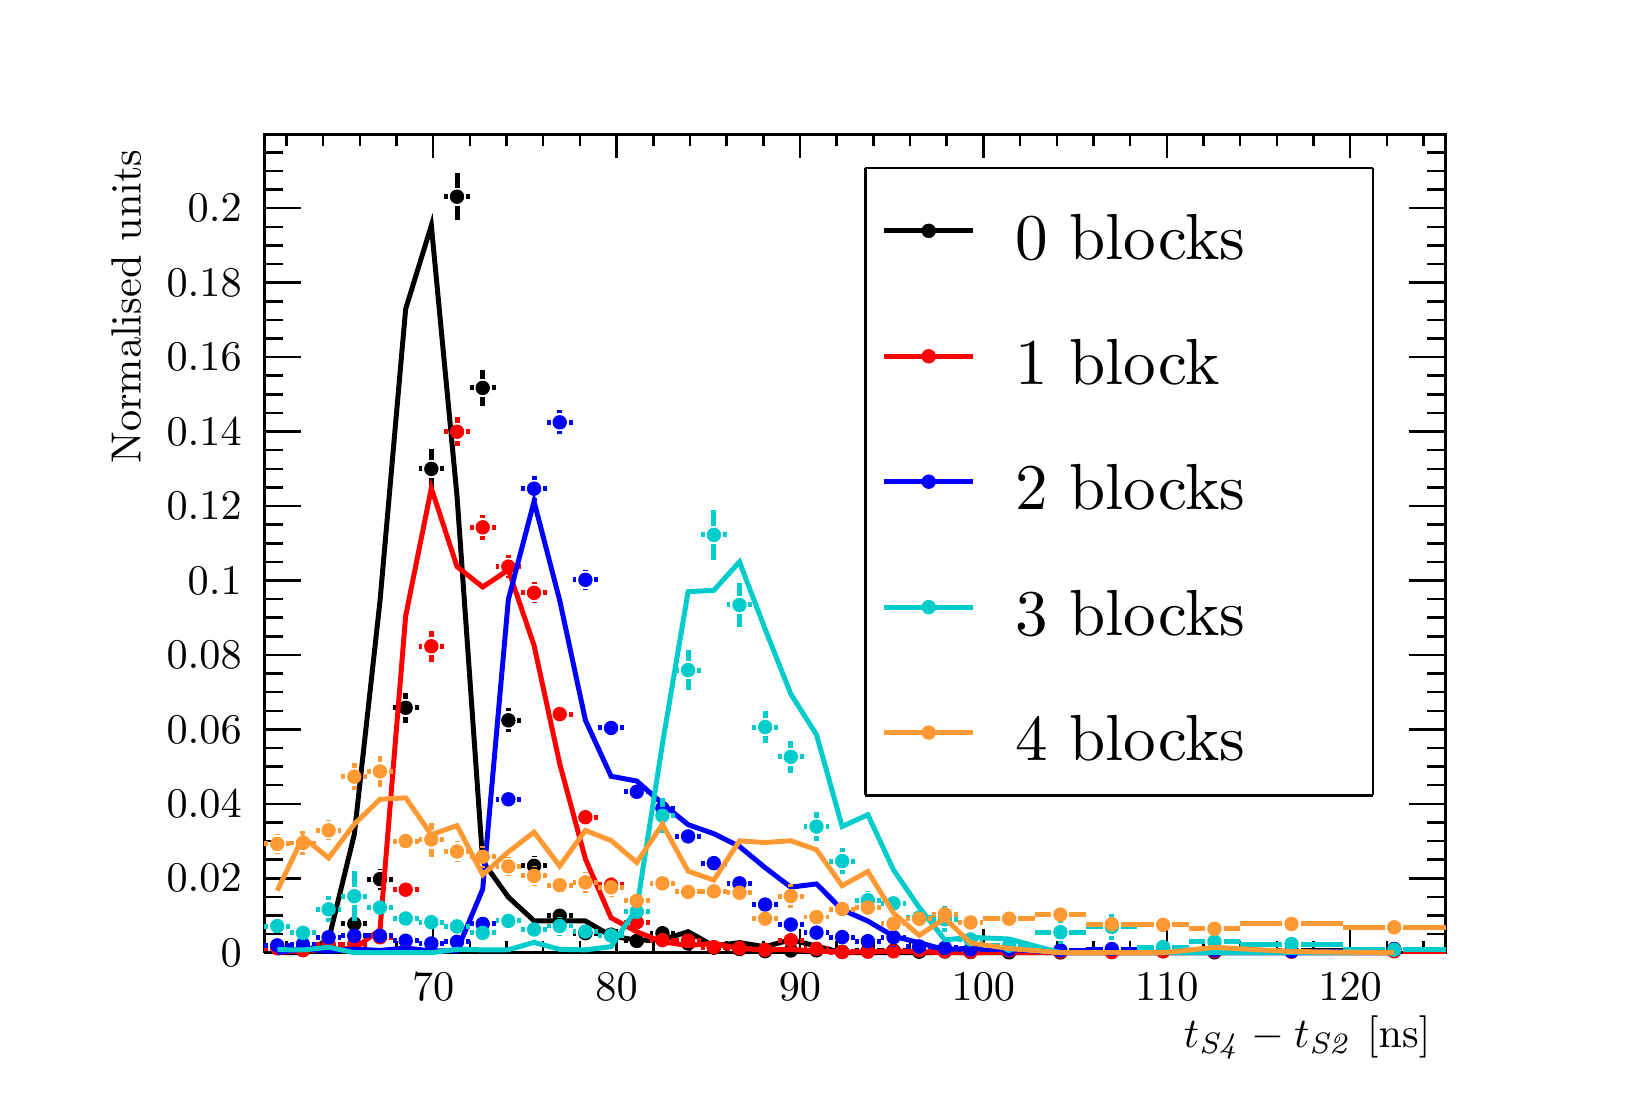
\begin{tikzpicture}
\pgfdeclareplotmark{cross} {
\pgfpathmoveto{\pgfpoint{-0.3\pgfplotmarksize}{\pgfplotmarksize}}
\pgfpathlineto{\pgfpoint{+0.3\pgfplotmarksize}{\pgfplotmarksize}}
\pgfpathlineto{\pgfpoint{+0.3\pgfplotmarksize}{0.3\pgfplotmarksize}}
\pgfpathlineto{\pgfpoint{+1\pgfplotmarksize}{0.3\pgfplotmarksize}}
\pgfpathlineto{\pgfpoint{+1\pgfplotmarksize}{-0.3\pgfplotmarksize}}
\pgfpathlineto{\pgfpoint{+0.3\pgfplotmarksize}{-0.3\pgfplotmarksize}}
\pgfpathlineto{\pgfpoint{+0.3\pgfplotmarksize}{-1.\pgfplotmarksize}}
\pgfpathlineto{\pgfpoint{-0.3\pgfplotmarksize}{-1.\pgfplotmarksize}}
\pgfpathlineto{\pgfpoint{-0.3\pgfplotmarksize}{-0.3\pgfplotmarksize}}
\pgfpathlineto{\pgfpoint{-1.\pgfplotmarksize}{-0.3\pgfplotmarksize}}
\pgfpathlineto{\pgfpoint{-1.\pgfplotmarksize}{0.3\pgfplotmarksize}}
\pgfpathlineto{\pgfpoint{-0.3\pgfplotmarksize}{0.3\pgfplotmarksize}}
\pgfpathclose
\pgfusepathqstroke
}
\pgfdeclareplotmark{cross*} {
\pgfpathmoveto{\pgfpoint{-0.3\pgfplotmarksize}{\pgfplotmarksize}}
\pgfpathlineto{\pgfpoint{+0.3\pgfplotmarksize}{\pgfplotmarksize}}
\pgfpathlineto{\pgfpoint{+0.3\pgfplotmarksize}{0.3\pgfplotmarksize}}
\pgfpathlineto{\pgfpoint{+1\pgfplotmarksize}{0.3\pgfplotmarksize}}
\pgfpathlineto{\pgfpoint{+1\pgfplotmarksize}{-0.3\pgfplotmarksize}}
\pgfpathlineto{\pgfpoint{+0.3\pgfplotmarksize}{-0.3\pgfplotmarksize}}
\pgfpathlineto{\pgfpoint{+0.3\pgfplotmarksize}{-1.\pgfplotmarksize}}
\pgfpathlineto{\pgfpoint{-0.3\pgfplotmarksize}{-1.\pgfplotmarksize}}
\pgfpathlineto{\pgfpoint{-0.3\pgfplotmarksize}{-0.3\pgfplotmarksize}}
\pgfpathlineto{\pgfpoint{-1.\pgfplotmarksize}{-0.3\pgfplotmarksize}}
\pgfpathlineto{\pgfpoint{-1.\pgfplotmarksize}{0.3\pgfplotmarksize}}
\pgfpathlineto{\pgfpoint{-0.3\pgfplotmarksize}{0.3\pgfplotmarksize}}
\pgfpathclose
\pgfusepathqfillstroke
}
\pgfdeclareplotmark{newstar} {
\pgfpathmoveto{\pgfqpoint{0pt}{\pgfplotmarksize}}
\pgfpathlineto{\pgfqpointpolar{44}{0.5\pgfplotmarksize}}
\pgfpathlineto{\pgfqpointpolar{18}{\pgfplotmarksize}}
\pgfpathlineto{\pgfqpointpolar{-20}{0.5\pgfplotmarksize}}
\pgfpathlineto{\pgfqpointpolar{-54}{\pgfplotmarksize}}
\pgfpathlineto{\pgfqpointpolar{-90}{0.5\pgfplotmarksize}}
\pgfpathlineto{\pgfqpointpolar{234}{\pgfplotmarksize}}
\pgfpathlineto{\pgfqpointpolar{198}{0.5\pgfplotmarksize}}
\pgfpathlineto{\pgfqpointpolar{162}{\pgfplotmarksize}}
\pgfpathlineto{\pgfqpointpolar{134}{0.5\pgfplotmarksize}}
\pgfpathclose
\pgfusepathqstroke
}
\pgfdeclareplotmark{newstar*} {
\pgfpathmoveto{\pgfqpoint{0pt}{\pgfplotmarksize}}
\pgfpathlineto{\pgfqpointpolar{44}{0.5\pgfplotmarksize}}
\pgfpathlineto{\pgfqpointpolar{18}{\pgfplotmarksize}}
\pgfpathlineto{\pgfqpointpolar{-20}{0.5\pgfplotmarksize}}
\pgfpathlineto{\pgfqpointpolar{-54}{\pgfplotmarksize}}
\pgfpathlineto{\pgfqpointpolar{-90}{0.5\pgfplotmarksize}}
\pgfpathlineto{\pgfqpointpolar{234}{\pgfplotmarksize}}
\pgfpathlineto{\pgfqpointpolar{198}{0.5\pgfplotmarksize}}
\pgfpathlineto{\pgfqpointpolar{162}{\pgfplotmarksize}}
\pgfpathlineto{\pgfqpointpolar{134}{0.5\pgfplotmarksize}}
\pgfpathclose
\pgfusepathqfillstroke
}
\definecolor{c}{rgb}{1,1,1};
\draw [color=c, fill=c] (0,0) rectangle (20,13.4957);
\draw [color=c, fill=c] (3,1.75444) rectangle (18,12.1461);
\definecolor{c}{rgb}{0,0,0};
\draw [c,line width=0.9] (3,1.75444) -- (3,12.1461) -- (18,12.1461) -- (18,1.75444) -- (3,1.75444);
\definecolor{c}{rgb}{1,1,1};
\draw [color=c, fill=c] (3,1.75444) rectangle (18,12.1461);
\definecolor{c}{rgb}{0,0,0};
\draw [c,line width=0.9] (3,1.75444) -- (3,12.1461) -- (18,12.1461) -- (18,1.75444) -- (3,1.75444);
\draw [c,line width=1.8] (3,1.83114) -- (3.04843,1.83114);
\draw [c,line width=1.8] (3.27766,1.83114) -- (3.32609,1.83114);
\foreach \P in {(3.16304,1.83114)}{\draw[mark options={color=c,fill=c},mark size=2.402402pt,mark=*] plot coordinates {\P};}
\draw [c,line width=1.8] (3.32609,1.82516) -- (3.37452,1.82516);
\draw [c,line width=1.8] (3.60374,1.82516) -- (3.65217,1.82516);
\foreach \P in {(3.48913,1.82516)}{\draw[mark options={color=c,fill=c},mark size=2.402402pt,mark=*] plot coordinates {\P};}
\draw [c,line width=1.8] (3.65217,1.84454) -- (3.7006,1.84454);
\draw [c,line width=1.8] (3.92983,1.84454) -- (3.97826,1.84454);
\foreach \P in {(3.81522,1.84454)}{\draw[mark options={color=c,fill=c},mark size=2.402402pt,mark=*] plot coordinates {\P};}
\draw [c,line width=1.8] (3.97826,2.12085) -- (4.02669,2.12085);
\draw [c,line width=1.8] (4.25592,2.12085) -- (4.30435,2.12085);
\foreach \P in {(4.1413,2.12085)}{\draw[mark options={color=c,fill=c},mark size=2.402402pt,mark=*] plot coordinates {\P};}
\draw [c,line width=1.8] (4.46739,2.55475) -- (4.46739,2.57465);
\draw [c,line width=1.8] (4.46739,2.80387) -- (4.46739,2.82376);
\draw [c,line width=1.8] (4.30435,2.68926) -- (4.35278,2.68926);
\draw [c,line width=1.8] (4.582,2.68926) -- (4.63043,2.68926);
\foreach \P in {(4.46739,2.68926)}{\draw[mark options={color=c,fill=c},mark size=2.402402pt,mark=*] plot coordinates {\P};}
\draw [c,line width=1.8] (4.79348,4.67286) -- (4.79348,4.75114);
\draw [c,line width=1.8] (4.79348,4.98037) -- (4.79348,5.05865);
\draw [c,line width=1.8] (4.63043,4.86575) -- (4.67886,4.86575);
\draw [c,line width=1.8] (4.90809,4.86575) -- (4.95652,4.86575);
\foreach \P in {(4.79348,4.86575)}{\draw[mark options={color=c,fill=c},mark size=2.402402pt,mark=*] plot coordinates {\P};}
\draw [c,line width=1.8] (5.11957,7.64548) -- (5.11957,7.78469);
\draw [c,line width=1.8] (5.11957,8.01391) -- (5.11957,8.15312);
\draw [c,line width=1.8] (4.95652,7.8993) -- (5.00495,7.8993);
\draw [c,line width=1.8] (5.23418,7.8993) -- (5.28261,7.8993);
\foreach \P in {(5.11957,7.8993)}{\draw[mark options={color=c,fill=c},mark size=2.402402pt,mark=*] plot coordinates {\P};}
\draw [c,line width=1.8] (5.44565,11.0614) -- (5.44565,11.2417);
\draw [c,line width=1.8] (5.44565,11.4709) -- (5.44565,11.6513);
\draw [c,line width=1.8] (5.28261,11.3563) -- (5.33104,11.3563);
\draw [c,line width=1.8] (5.56027,11.3563) -- (5.6087,11.3563);
\foreach \P in {(5.44565,11.3563)}{\draw[mark options={color=c,fill=c},mark size=2.402402pt,mark=*] plot coordinates {\P};}
\draw [c,line width=1.8] (5.77174,8.694) -- (5.77174,8.81308);
\draw [c,line width=1.8] (5.77174,9.04231) -- (5.77174,9.1614);
\draw [c,line width=1.8] (5.6087,8.9277) -- (5.65713,8.9277);
\draw [c,line width=1.8] (5.88635,8.9277) -- (5.93478,8.9277);
\foreach \P in {(5.77174,8.9277)}{\draw[mark options={color=c,fill=c},mark size=2.402402pt,mark=*] plot coordinates {\P};}
\draw [c,line width=1.8] (6.09783,4.55419) -- (6.09783,4.59147);
\draw [c,line width=1.8] (6.09783,4.8207) -- (6.09783,4.85798);
\draw [c,line width=1.8] (5.93478,4.70608) -- (5.98321,4.70608);
\draw [c,line width=1.8] (6.21244,4.70608) -- (6.26087,4.70608);
\foreach \P in {(6.09783,4.70608)}{\draw[mark options={color=c,fill=c},mark size=2.402402pt,mark=*] plot coordinates {\P};}
\draw [c,line width=1.8] (6.42391,2.73278) -- (6.42391,2.74337);
\draw [c,line width=1.8] (6.42391,2.9726) -- (6.42391,2.98319);
\draw [c,line width=1.8] (6.26087,2.85799) -- (6.3093,2.85799);
\draw [c,line width=1.8] (6.53853,2.85799) -- (6.58696,2.85799);
\foreach \P in {(6.42391,2.85799)}{\draw[mark options={color=c,fill=c},mark size=2.402402pt,mark=*] plot coordinates {\P};}
\draw [c,line width=1.8] (6.58696,2.22344) -- (6.63539,2.22344);
\draw [c,line width=1.8] (6.86461,2.22344) -- (6.91304,2.22344);
\foreach \P in {(6.75,2.22344)}{\draw[mark options={color=c,fill=c},mark size=2.402402pt,mark=*] plot coordinates {\P};}
\draw [c,line width=1.8] (6.91304,2.00306) -- (6.96147,2.00306);
\draw [c,line width=1.8] (7.1907,2.00306) -- (7.23913,2.00306);
\foreach \P in {(7.07609,2.00306)}{\draw[mark options={color=c,fill=c},mark size=2.402402pt,mark=*] plot coordinates {\P};}
\draw [c,line width=1.8] (7.23913,1.98414) -- (7.28756,1.98414);
\draw [c,line width=1.8] (7.51679,1.98414) -- (7.56522,1.98414);
\foreach \P in {(7.40217,1.98414)}{\draw[mark options={color=c,fill=c},mark size=2.402402pt,mark=*] plot coordinates {\P};}
\draw [c,line width=1.8] (7.56522,1.90433) -- (7.61365,1.90433);
\draw [c,line width=1.8] (7.84287,1.90433) -- (7.8913,1.90433);
\foreach \P in {(7.72826,1.90433)}{\draw[mark options={color=c,fill=c},mark size=2.402402pt,mark=*] plot coordinates {\P};}
\draw [c,line width=1.8] (7.8913,2.00177) -- (7.93973,2.00177);
\draw [c,line width=1.8] (8.16896,2.00177) -- (8.21739,2.00177);
\foreach \P in {(8.05435,2.00177)}{\draw[mark options={color=c,fill=c},mark size=2.402402pt,mark=*] plot coordinates {\P};}
\draw [c,line width=1.8] (8.21739,1.87216) -- (8.26582,1.87216);
\draw [c,line width=1.8] (8.49505,1.87216) -- (8.54348,1.87216);
\foreach \P in {(8.38043,1.87216)}{\draw[mark options={color=c,fill=c},mark size=2.402402pt,mark=*] plot coordinates {\P};}
\draw [c,line width=1.8] (8.54348,1.81906) -- (8.59191,1.81906);
\draw [c,line width=1.8] (8.82113,1.81906) -- (8.86957,1.81906);
\foreach \P in {(8.70652,1.81906)}{\draw[mark options={color=c,fill=c},mark size=2.402402pt,mark=*] plot coordinates {\P};}
\draw [c,line width=1.8] (8.86957,1.80095) -- (8.918,1.80095);
\draw [c,line width=1.8] (9.14722,1.80095) -- (9.19565,1.80095);
\foreach \P in {(9.03261,1.80095)}{\draw[mark options={color=c,fill=c},mark size=2.402402pt,mark=*] plot coordinates {\P};}
\draw [c,line width=1.8] (9.19565,1.77486) -- (9.24408,1.77486);
\draw [c,line width=1.8] (9.47331,1.77486) -- (9.52174,1.77486);
\foreach \P in {(9.3587,1.77486)}{\draw[mark options={color=c,fill=c},mark size=2.402402pt,mark=*] plot coordinates {\P};}
\draw [c,line width=1.8] (9.52174,1.78306) -- (9.57017,1.78306);
\draw [c,line width=1.8] (9.7994,1.78306) -- (9.84783,1.78306);
\foreach \P in {(9.68478,1.78306)}{\draw[mark options={color=c,fill=c},mark size=2.402402pt,mark=*] plot coordinates {\P};}
\draw [c,line width=1.8] (9.84783,1.78487) -- (9.89626,1.78487);
\draw [c,line width=1.8] (10.1255,1.78487) -- (10.1739,1.78487);
\foreach \P in {(10.0109,1.78487)}{\draw[mark options={color=c,fill=c},mark size=2.402402pt,mark=*] plot coordinates {\P};}
\draw [c,line width=1.8] (10.1739,1.76533) -- (10.2223,1.76533);
\draw [c,line width=1.8] (10.4516,1.76533) -- (10.5,1.76533);
\foreach \P in {(10.337,1.76533)}{\draw[mark options={color=c,fill=c},mark size=2.402402pt,mark=*] plot coordinates {\P};}
\draw [c,line width=1.8] (10.5,1.7786) -- (10.5484,1.7786);
\draw [c,line width=1.8] (10.7777,1.7786) -- (10.8261,1.7786);
\foreach \P in {(10.663,1.7786)}{\draw[mark options={color=c,fill=c},mark size=2.402402pt,mark=*] plot coordinates {\P};}
\draw [c,line width=1.8] (10.8261,1.78124) -- (10.8745,1.78124);
\draw [c,line width=1.8] (11.1037,1.78124) -- (11.1522,1.78124);
\foreach \P in {(10.9891,1.78124)}{\draw[mark options={color=c,fill=c},mark size=2.402402pt,mark=*] plot coordinates {\P};}
\draw [c,line width=1.8] (11.1522,1.767) -- (11.2006,1.767);
\draw [c,line width=1.8] (11.4298,1.767) -- (11.4783,1.767);
\foreach \P in {(11.3152,1.767)}{\draw[mark options={color=c,fill=c},mark size=2.402402pt,mark=*] plot coordinates {\P};}
\draw [c,line width=1.8] (11.4783,1.77006) -- (11.5267,1.77006);
\draw [c,line width=1.8] (11.7559,1.77006) -- (11.8043,1.77006);
\foreach \P in {(11.6413,1.77006)}{\draw[mark options={color=c,fill=c},mark size=2.402402pt,mark=*] plot coordinates {\P};}
\draw [c,line width=1.8] (11.8043,1.76448) -- (11.8528,1.76448);
\draw [c,line width=1.8] (12.082,1.76448) -- (12.1304,1.76448);
\foreach \P in {(11.9674,1.76448)}{\draw[mark options={color=c,fill=c},mark size=2.402402pt,mark=*] plot coordinates {\P};}
\draw [c,line width=1.8] (12.1304,1.76013) -- (12.3419,1.76013);
\draw [c,line width=1.8] (12.5711,1.76013) -- (12.7826,1.76013);
\foreach \P in {(12.4565,1.76013)}{\draw[mark options={color=c,fill=c},mark size=2.402402pt,mark=*] plot coordinates {\P};}
\draw [c,line width=1.8] (12.7826,1.75877) -- (12.9941,1.75877);
\draw [c,line width=1.8] (13.2233,1.75877) -- (13.4348,1.75877);
\foreach \P in {(13.1087,1.75877)}{\draw[mark options={color=c,fill=c},mark size=2.402402pt,mark=*] plot coordinates {\P};}
\draw [c,line width=1.8] (13.4348,1.7716) -- (13.6463,1.7716);
\draw [c,line width=1.8] (13.8755,1.7716) -- (14.087,1.7716);
\foreach \P in {(13.7609,1.7716)}{\draw[mark options={color=c,fill=c},mark size=2.402402pt,mark=*] plot coordinates {\P};}
\draw [c,line width=1.8] (14.087,1.77325) -- (14.2984,1.77325);
\draw [c,line width=1.8] (14.5277,1.77325) -- (14.7391,1.77325);
\foreach \P in {(14.413,1.77325)}{\draw[mark options={color=c,fill=c},mark size=2.402402pt,mark=*] plot coordinates {\P};}
\draw [c,line width=1.8] (14.7391,1.76012) -- (14.9506,1.76012);
\draw [c,line width=1.8] (15.1798,1.76012) -- (15.3913,1.76012);
\foreach \P in {(15.0652,1.76012)}{\draw[mark options={color=c,fill=c},mark size=2.402402pt,mark=*] plot coordinates {\P};}
\draw [c,line width=1.8] (15.3913,1.77863) -- (15.9289,1.77863);
\draw [c,line width=1.8] (16.1581,1.77863) -- (16.6957,1.77863);
\foreach \P in {(16.0435,1.77863)}{\draw[mark options={color=c,fill=c},mark size=2.402402pt,mark=*] plot coordinates {\P};}
\draw [c,line width=1.8] (16.6957,1.80192) -- (17.2332,1.80192);
\draw [c,line width=1.8] (17.4624,1.80192) -- (18,1.80192);
\foreach \P in {(17.3478,1.80192)}{\draw[mark options={color=c,fill=c},mark size=2.402402pt,mark=*] plot coordinates {\P};}
\draw [c,line width=0.9] (3,1.75444) -- (18,1.75444);
\draw [c,line width=0.9] (5.14286,2.05809) -- (5.14286,1.75444);
\draw [c,line width=0.9] (5.6087,1.90627) -- (5.6087,1.75444);
\draw [c,line width=0.9] (6.07453,1.90627) -- (6.07453,1.75444);
\draw [c,line width=0.9] (6.54037,1.90627) -- (6.54037,1.75444);
\draw [c,line width=0.9] (7.00621,1.90627) -- (7.00621,1.75444);
\draw [c,line width=0.9] (7.47205,2.05809) -- (7.47205,1.75444);
\draw [c,line width=0.9] (7.93789,1.90627) -- (7.93789,1.75444);
\draw [c,line width=0.9] (8.40373,1.90627) -- (8.40373,1.75444);
\draw [c,line width=0.9] (8.86957,1.90627) -- (8.86957,1.75444);
\draw [c,line width=0.9] (9.3354,1.90627) -- (9.3354,1.75444);
\draw [c,line width=0.9] (9.80124,2.05809) -- (9.80124,1.75444);
\draw [c,line width=0.9] (10.2671,1.90627) -- (10.2671,1.75444);
\draw [c,line width=0.9] (10.7329,1.90627) -- (10.7329,1.75444);
\draw [c,line width=0.9] (11.1988,1.90627) -- (11.1988,1.75444);
\draw [c,line width=0.9] (11.6646,1.90627) -- (11.6646,1.75444);
\draw [c,line width=0.9] (12.1304,2.05809) -- (12.1304,1.75444);
\draw [c,line width=0.9] (12.5963,1.90627) -- (12.5963,1.75444);
\draw [c,line width=0.9] (13.0621,1.90627) -- (13.0621,1.75444);
\draw [c,line width=0.9] (13.528,1.90627) -- (13.528,1.75444);
\draw [c,line width=0.9] (13.9938,1.90627) -- (13.9938,1.75444);
\draw [c,line width=0.9] (14.4596,2.05809) -- (14.4596,1.75444);
\draw [c,line width=0.9] (14.9255,1.90627) -- (14.9255,1.75444);
\draw [c,line width=0.9] (15.3913,1.90627) -- (15.3913,1.75444);
\draw [c,line width=0.9] (15.8571,1.90627) -- (15.8571,1.75444);
\draw [c,line width=0.9] (16.323,1.90627) -- (16.323,1.75444);
\draw [c,line width=0.9] (16.7888,2.05809) -- (16.7888,1.75444);
\draw [c,line width=0.9] (5.14286,2.05809) -- (5.14286,1.75444);
\draw [c,line width=0.9] (4.67702,1.90627) -- (4.67702,1.75444);
\draw [c,line width=0.9] (4.21118,1.90627) -- (4.21118,1.75444);
\draw [c,line width=0.9] (3.74534,1.90627) -- (3.74534,1.75444);
\draw [c,line width=0.9] (3.2795,1.90627) -- (3.2795,1.75444);
\draw [c,line width=0.9] (16.7888,2.05809) -- (16.7888,1.75444);
\draw [c,line width=0.9] (17.2547,1.90627) -- (17.2547,1.75444);
\draw [c,line width=0.9] (17.7205,1.90627) -- (17.7205,1.75444);
\draw [anchor=base] (5.14286,1.14713) node[scale=1.52731, color=c, rotate=0]{70};
\draw [anchor=base] (7.47205,1.14713) node[scale=1.52731, color=c, rotate=0]{80};
\draw [anchor=base] (9.80124,1.14713) node[scale=1.52731, color=c, rotate=0]{90};
\draw [anchor=base] (12.1304,1.14713) node[scale=1.52731, color=c, rotate=0]{100};
\draw [anchor=base] (14.4596,1.14713) node[scale=1.52731, color=c, rotate=0]{110};
\draw [anchor=base] (16.7888,1.14713) node[scale=1.52731, color=c, rotate=0]{120};
\draw [anchor= east] (18,0.674785) node[scale=1.52731, color=c, rotate=0]{$t_{\mathit{S4}} - t_{\mathit{S2}}$ [ns]};
\draw [c,line width=0.9] (3,12.1461) -- (18,12.1461);
\draw [c,line width=0.9] (5.14286,11.8425) -- (5.14286,12.1461);
\draw [c,line width=0.9] (5.6087,11.9943) -- (5.6087,12.1461);
\draw [c,line width=0.9] (6.07453,11.9943) -- (6.07453,12.1461);
\draw [c,line width=0.9] (6.54037,11.9943) -- (6.54037,12.1461);
\draw [c,line width=0.9] (7.00621,11.9943) -- (7.00621,12.1461);
\draw [c,line width=0.9] (7.47205,11.8425) -- (7.47205,12.1461);
\draw [c,line width=0.9] (7.93789,11.9943) -- (7.93789,12.1461);
\draw [c,line width=0.9] (8.40373,11.9943) -- (8.40373,12.1461);
\draw [c,line width=0.9] (8.86957,11.9943) -- (8.86957,12.1461);
\draw [c,line width=0.9] (9.3354,11.9943) -- (9.3354,12.1461);
\draw [c,line width=0.9] (9.80124,11.8425) -- (9.80124,12.1461);
\draw [c,line width=0.9] (10.2671,11.9943) -- (10.2671,12.1461);
\draw [c,line width=0.9] (10.7329,11.9943) -- (10.7329,12.1461);
\draw [c,line width=0.9] (11.1988,11.9943) -- (11.1988,12.1461);
\draw [c,line width=0.9] (11.6646,11.9943) -- (11.6646,12.1461);
\draw [c,line width=0.9] (12.1304,11.8425) -- (12.1304,12.1461);
\draw [c,line width=0.9] (12.5963,11.9943) -- (12.5963,12.1461);
\draw [c,line width=0.9] (13.0621,11.9943) -- (13.0621,12.1461);
\draw [c,line width=0.9] (13.528,11.9943) -- (13.528,12.1461);
\draw [c,line width=0.9] (13.9938,11.9943) -- (13.9938,12.1461);
\draw [c,line width=0.9] (14.4596,11.8425) -- (14.4596,12.1461);
\draw [c,line width=0.9] (14.9255,11.9943) -- (14.9255,12.1461);
\draw [c,line width=0.9] (15.3913,11.9943) -- (15.3913,12.1461);
\draw [c,line width=0.9] (15.8571,11.9943) -- (15.8571,12.1461);
\draw [c,line width=0.9] (16.323,11.9943) -- (16.323,12.1461);
\draw [c,line width=0.9] (16.7888,11.8425) -- (16.7888,12.1461);
\draw [c,line width=0.9] (5.14286,11.8425) -- (5.14286,12.1461);
\draw [c,line width=0.9] (4.67702,11.9943) -- (4.67702,12.1461);
\draw [c,line width=0.9] (4.21118,11.9943) -- (4.21118,12.1461);
\draw [c,line width=0.9] (3.74534,11.9943) -- (3.74534,12.1461);
\draw [c,line width=0.9] (3.2795,11.9943) -- (3.2795,12.1461);
\draw [c,line width=0.9] (16.7888,11.8425) -- (16.7888,12.1461);
\draw [c,line width=0.9] (17.2547,11.9943) -- (17.2547,12.1461);
\draw [c,line width=0.9] (17.7205,11.9943) -- (17.7205,12.1461);
\draw [c,line width=0.9] (3,1.75444) -- (3,12.1461);
\draw [c,line width=0.9] (3.462,1.75444) -- (3,1.75444);
\draw [c,line width=0.9] (3.231,1.99082) -- (3,1.99082);
\draw [c,line width=0.9] (3.231,2.2272) -- (3,2.2272);
\draw [c,line width=0.9] (3.231,2.46357) -- (3,2.46357);
\draw [c,line width=0.9] (3.462,2.69995) -- (3,2.69995);
\draw [c,line width=0.9] (3.231,2.93633) -- (3,2.93633);
\draw [c,line width=0.9] (3.231,3.1727) -- (3,3.1727);
\draw [c,line width=0.9] (3.231,3.40908) -- (3,3.40908);
\draw [c,line width=0.9] (3.462,3.64546) -- (3,3.64546);
\draw [c,line width=0.9] (3.231,3.88184) -- (3,3.88184);
\draw [c,line width=0.9] (3.231,4.11821) -- (3,4.11821);
\draw [c,line width=0.9] (3.231,4.35459) -- (3,4.35459);
\draw [c,line width=0.9] (3.462,4.59097) -- (3,4.59097);
\draw [c,line width=0.9] (3.231,4.82734) -- (3,4.82734);
\draw [c,line width=0.9] (3.231,5.06372) -- (3,5.06372);
\draw [c,line width=0.9] (3.231,5.3001) -- (3,5.3001);
\draw [c,line width=0.9] (3.462,5.53648) -- (3,5.53648);
\draw [c,line width=0.9] (3.231,5.77285) -- (3,5.77285);
\draw [c,line width=0.9] (3.231,6.00923) -- (3,6.00923);
\draw [c,line width=0.9] (3.231,6.24561) -- (3,6.24561);
\draw [c,line width=0.9] (3.462,6.48199) -- (3,6.48199);
\draw [c,line width=0.9] (3.231,6.71836) -- (3,6.71836);
\draw [c,line width=0.9] (3.231,6.95474) -- (3,6.95474);
\draw [c,line width=0.9] (3.231,7.19112) -- (3,7.19112);
\draw [c,line width=0.9] (3.462,7.42749) -- (3,7.42749);
\draw [c,line width=0.9] (3.231,7.66387) -- (3,7.66387);
\draw [c,line width=0.9] (3.231,7.90025) -- (3,7.90025);
\draw [c,line width=0.9] (3.231,8.13663) -- (3,8.13663);
\draw [c,line width=0.9] (3.462,8.373) -- (3,8.373);
\draw [c,line width=0.9] (3.231,8.60938) -- (3,8.60938);
\draw [c,line width=0.9] (3.231,8.84576) -- (3,8.84576);
\draw [c,line width=0.9] (3.231,9.08213) -- (3,9.08213);
\draw [c,line width=0.9] (3.462,9.31851) -- (3,9.31851);
\draw [c,line width=0.9] (3.231,9.55489) -- (3,9.55489);
\draw [c,line width=0.9] (3.231,9.79127) -- (3,9.79127);
\draw [c,line width=0.9] (3.231,10.0276) -- (3,10.0276);
\draw [c,line width=0.9] (3.462,10.264) -- (3,10.264);
\draw [c,line width=0.9] (3.231,10.5004) -- (3,10.5004);
\draw [c,line width=0.9] (3.231,10.7368) -- (3,10.7368);
\draw [c,line width=0.9] (3.231,10.9732) -- (3,10.9732);
\draw [c,line width=0.9] (3.462,11.2095) -- (3,11.2095);
\draw [c,line width=0.9] (3.462,11.2095) -- (3,11.2095);
\draw [c,line width=0.9] (3.231,11.4459) -- (3,11.4459);
\draw [c,line width=0.9] (3.231,11.6823) -- (3,11.6823);
\draw [c,line width=0.9] (3.231,11.9187) -- (3,11.9187);
\draw [anchor= east] (2.9,1.75444) node[scale=1.52731, color=c, rotate=0]{0};
\draw [anchor= east] (2.9,2.69995) node[scale=1.52731, color=c, rotate=0]{0.02};
\draw [anchor= east] (2.9,3.64546) node[scale=1.52731, color=c, rotate=0]{0.04};
\draw [anchor= east] (2.9,4.59097) node[scale=1.52731, color=c, rotate=0]{0.06};
\draw [anchor= east] (2.9,5.53648) node[scale=1.52731, color=c, rotate=0]{0.08};
\draw [anchor= east] (2.9,6.48199) node[scale=1.52731, color=c, rotate=0]{0.1};
\draw [anchor= east] (2.9,7.42749) node[scale=1.52731, color=c, rotate=0]{0.12};
\draw [anchor= east] (2.9,8.373) node[scale=1.52731, color=c, rotate=0]{0.14};
\draw [anchor= east] (2.9,9.31851) node[scale=1.52731, color=c, rotate=0]{0.16};
\draw [anchor= east] (2.9,10.264) node[scale=1.52731, color=c, rotate=0]{0.18};
\draw [anchor= east] (2.9,11.2095) node[scale=1.52731, color=c, rotate=0]{0.2};
\draw [anchor= east] (1.24,12.1461) node[scale=1.52731, color=c, rotate=90]{Normalised units};
\draw [c,line width=0.9] (18,1.75444) -- (18,12.1461);
\draw [c,line width=0.9] (17.538,1.75444) -- (18,1.75444);
\draw [c,line width=0.9] (17.769,1.99082) -- (18,1.99082);
\draw [c,line width=0.9] (17.769,2.2272) -- (18,2.2272);
\draw [c,line width=0.9] (17.769,2.46357) -- (18,2.46357);
\draw [c,line width=0.9] (17.538,2.69995) -- (18,2.69995);
\draw [c,line width=0.9] (17.769,2.93633) -- (18,2.93633);
\draw [c,line width=0.9] (17.769,3.1727) -- (18,3.1727);
\draw [c,line width=0.9] (17.769,3.40908) -- (18,3.40908);
\draw [c,line width=0.9] (17.538,3.64546) -- (18,3.64546);
\draw [c,line width=0.9] (17.769,3.88184) -- (18,3.88184);
\draw [c,line width=0.9] (17.769,4.11821) -- (18,4.11821);
\draw [c,line width=0.9] (17.769,4.35459) -- (18,4.35459);
\draw [c,line width=0.9] (17.538,4.59097) -- (18,4.59097);
\draw [c,line width=0.9] (17.769,4.82734) -- (18,4.82734);
\draw [c,line width=0.9] (17.769,5.06372) -- (18,5.06372);
\draw [c,line width=0.9] (17.769,5.3001) -- (18,5.3001);
\draw [c,line width=0.9] (17.538,5.53648) -- (18,5.53648);
\draw [c,line width=0.9] (17.769,5.77285) -- (18,5.77285);
\draw [c,line width=0.9] (17.769,6.00923) -- (18,6.00923);
\draw [c,line width=0.9] (17.769,6.24561) -- (18,6.24561);
\draw [c,line width=0.9] (17.538,6.48199) -- (18,6.48199);
\draw [c,line width=0.9] (17.769,6.71836) -- (18,6.71836);
\draw [c,line width=0.9] (17.769,6.95474) -- (18,6.95474);
\draw [c,line width=0.9] (17.769,7.19112) -- (18,7.19112);
\draw [c,line width=0.9] (17.538,7.42749) -- (18,7.42749);
\draw [c,line width=0.9] (17.769,7.66387) -- (18,7.66387);
\draw [c,line width=0.9] (17.769,7.90025) -- (18,7.90025);
\draw [c,line width=0.9] (17.769,8.13663) -- (18,8.13663);
\draw [c,line width=0.9] (17.538,8.373) -- (18,8.373);
\draw [c,line width=0.9] (17.769,8.60938) -- (18,8.60938);
\draw [c,line width=0.9] (17.769,8.84576) -- (18,8.84576);
\draw [c,line width=0.9] (17.769,9.08213) -- (18,9.08213);
\draw [c,line width=0.9] (17.538,9.31851) -- (18,9.31851);
\draw [c,line width=0.9] (17.769,9.55489) -- (18,9.55489);
\draw [c,line width=0.9] (17.769,9.79127) -- (18,9.79127);
\draw [c,line width=0.9] (17.769,10.0276) -- (18,10.0276);
\draw [c,line width=0.9] (17.538,10.264) -- (18,10.264);
\draw [c,line width=0.9] (17.769,10.5004) -- (18,10.5004);
\draw [c,line width=0.9] (17.769,10.7368) -- (18,10.7368);
\draw [c,line width=0.9] (17.769,10.9732) -- (18,10.9732);
\draw [c,line width=0.9] (17.538,11.2095) -- (18,11.2095);
\draw [c,line width=0.9] (17.538,11.2095) -- (18,11.2095);
\draw [c,line width=0.9] (17.769,11.4459) -- (18,11.4459);
\draw [c,line width=0.9] (17.769,11.6823) -- (18,11.6823);
\draw [c,line width=0.9] (17.769,11.9187) -- (18,11.9187);
\draw [c,line width=1.8] (3.16304,1.75444) -- (3.48913,1.75444) -- (3.81522,1.91963) -- (4.1413,3.2586) -- (4.46739,6.21923) -- (4.79348,9.93097) -- (5.11957,10.9903) -- (5.44565,7.5521) -- (5.77174,2.91629) -- (6.09783,2.46021) -- (6.42391,2.16031)
 -- (6.75,2.15888) -- (7.07609,2.1576) -- (7.40217,1.96821) -- (7.72826,1.91351) -- (8.05435,1.91827) -- (8.38043,2.02123) -- (8.70652,1.84056) -- (9.03261,1.88256) -- (9.3587,1.83017) -- (9.68478,1.92059) -- (10.0109,1.83781) -- (10.337,1.75444) --
 (10.663,1.75444) -- (10.9891,1.75444) -- (11.3152,1.75444) -- (11.6413,1.75444) -- (11.9674,1.75444) -- (12.4565,1.75444) -- (13.1087,1.75444) -- (13.7609,1.75444) -- (14.413,1.75444) -- (15.0652,1.75444) -- (16.0435,1.75444) -- (17.3478,1.75444);
\definecolor{c}{rgb}{1,0,0};
\draw [c,line width=1.8] (3,1.81211) -- (3.04843,1.81211);
\draw [c,line width=1.8] (3.27766,1.81211) -- (3.32609,1.81211);
\foreach \P in {(3.16304,1.81211)}{\draw[mark options={color=c,fill=c},mark size=2.402402pt,mark=*] plot coordinates {\P};}
\draw [c,line width=1.8] (3.32609,1.78648) -- (3.37452,1.78648);
\draw [c,line width=1.8] (3.60374,1.78648) -- (3.65217,1.78648);
\foreach \P in {(3.48913,1.78648)}{\draw[mark options={color=c,fill=c},mark size=2.402402pt,mark=*] plot coordinates {\P};}
\draw [c,line width=1.8] (3.65217,1.86159) -- (3.7006,1.86159);
\draw [c,line width=1.8] (3.92983,1.86159) -- (3.97826,1.86159);
\foreach \P in {(3.81522,1.86159)}{\draw[mark options={color=c,fill=c},mark size=2.402402pt,mark=*] plot coordinates {\P};}
\draw [c,line width=1.8] (3.97826,1.86397) -- (4.02669,1.86397);
\draw [c,line width=1.8] (4.25592,1.86397) -- (4.30435,1.86397);
\foreach \P in {(4.1413,1.86397)}{\draw[mark options={color=c,fill=c},mark size=2.402402pt,mark=*] plot coordinates {\P};}
\draw [c,line width=1.8] (4.30435,1.95008) -- (4.35278,1.95008);
\draw [c,line width=1.8] (4.582,1.95008) -- (4.63043,1.95008);
\foreach \P in {(4.46739,1.95008)}{\draw[mark options={color=c,fill=c},mark size=2.402402pt,mark=*] plot coordinates {\P};}
\draw [c,line width=1.8] (4.63043,2.55497) -- (4.67886,2.55497);
\draw [c,line width=1.8] (4.90809,2.55497) -- (4.95652,2.55497);
\foreach \P in {(4.79348,2.55497)}{\draw[mark options={color=c,fill=c},mark size=2.402402pt,mark=*] plot coordinates {\P};}
\draw [c,line width=1.8] (5.11957,5.44535) -- (5.11957,5.53144);
\draw [c,line width=1.8] (5.11957,5.76067) -- (5.11957,5.84676);
\draw [c,line width=1.8] (4.95652,5.64606) -- (5.00495,5.64606);
\draw [c,line width=1.8] (5.23418,5.64606) -- (5.28261,5.64606);
\foreach \P in {(5.11957,5.64606)}{\draw[mark options={color=c,fill=c},mark size=2.402402pt,mark=*] plot coordinates {\P};}
\draw [c,line width=1.8] (5.44565,8.18679) -- (5.44565,8.25649);
\draw [c,line width=1.8] (5.44565,8.48571) -- (5.44565,8.55541);
\draw [c,line width=1.8] (5.28261,8.3711) -- (5.33104,8.3711);
\draw [c,line width=1.8] (5.56027,8.3711) -- (5.6087,8.3711);
\foreach \P in {(5.44565,8.3711)}{\draw[mark options={color=c,fill=c},mark size=2.402402pt,mark=*] plot coordinates {\P};}
\draw [c,line width=1.8] (5.77174,6.99625) -- (5.77174,7.04232);
\draw [c,line width=1.8] (5.77174,7.27155) -- (5.77174,7.31762);
\draw [c,line width=1.8] (5.6087,7.15694) -- (5.65713,7.15694);
\draw [c,line width=1.8] (5.88635,7.15694) -- (5.93478,7.15694);
\foreach \P in {(5.77174,7.15694)}{\draw[mark options={color=c,fill=c},mark size=2.402402pt,mark=*] plot coordinates {\P};}
\draw [c,line width=1.8] (6.09783,6.51144) -- (6.09783,6.54373);
\draw [c,line width=1.8] (6.09783,6.77295) -- (6.09783,6.80523);
\draw [c,line width=1.8] (5.93478,6.65834) -- (5.98321,6.65834);
\draw [c,line width=1.8] (6.21244,6.65834) -- (6.26087,6.65834);
\foreach \P in {(6.09783,6.65834)}{\draw[mark options={color=c,fill=c},mark size=2.402402pt,mark=*] plot coordinates {\P};}
\draw [c,line width=1.8] (6.42391,6.19165) -- (6.42391,6.21023);
\draw [c,line width=1.8] (6.42391,6.43946) -- (6.42391,6.45803);
\draw [c,line width=1.8] (6.26087,6.32484) -- (6.3093,6.32484);
\draw [c,line width=1.8] (6.53853,6.32484) -- (6.58696,6.32484);
\foreach \P in {(6.42391,6.32484)}{\draw[mark options={color=c,fill=c},mark size=2.402402pt,mark=*] plot coordinates {\P};}
\draw [c,line width=1.8] (6.58696,4.78522) -- (6.63539,4.78522);
\draw [c,line width=1.8] (6.86461,4.78522) -- (6.91304,4.78522);
\foreach \P in {(6.75,4.78522)}{\draw[mark options={color=c,fill=c},mark size=2.402402pt,mark=*] plot coordinates {\P};}
\draw [c,line width=1.8] (6.91304,3.47547) -- (6.96147,3.47547);
\draw [c,line width=1.8] (7.1907,3.47547) -- (7.23913,3.47547);
\foreach \P in {(7.07609,3.47547)}{\draw[mark options={color=c,fill=c},mark size=2.402402pt,mark=*] plot coordinates {\P};}
\draw [c,line width=1.8] (7.23913,2.61559) -- (7.28756,2.61559);
\draw [c,line width=1.8] (7.51679,2.61559) -- (7.56522,2.61559);
\foreach \P in {(7.40217,2.61559)}{\draw[mark options={color=c,fill=c},mark size=2.402402pt,mark=*] plot coordinates {\P};}
\draw [c,line width=1.8] (7.56522,2.14104) -- (7.61365,2.14104);
\draw [c,line width=1.8] (7.84287,2.14104) -- (7.8913,2.14104);
\foreach \P in {(7.72826,2.14104)}{\draw[mark options={color=c,fill=c},mark size=2.402402pt,mark=*] plot coordinates {\P};}
\draw [c,line width=1.8] (7.8913,1.91483) -- (7.93973,1.91483);
\draw [c,line width=1.8] (8.16896,1.91483) -- (8.21739,1.91483);
\foreach \P in {(8.05435,1.91483)}{\draw[mark options={color=c,fill=c},mark size=2.402402pt,mark=*] plot coordinates {\P};}
\draw [c,line width=1.8] (8.21739,1.90786) -- (8.26582,1.90786);
\draw [c,line width=1.8] (8.49505,1.90786) -- (8.54348,1.90786);
\foreach \P in {(8.38043,1.90786)}{\draw[mark options={color=c,fill=c},mark size=2.402402pt,mark=*] plot coordinates {\P};}
\draw [c,line width=1.8] (8.54348,1.82528) -- (8.59191,1.82528);
\draw [c,line width=1.8] (8.82113,1.82528) -- (8.86957,1.82528);
\foreach \P in {(8.70652,1.82528)}{\draw[mark options={color=c,fill=c},mark size=2.402402pt,mark=*] plot coordinates {\P};}
\draw [c,line width=1.8] (8.86957,1.81201) -- (8.918,1.81201);
\draw [c,line width=1.8] (9.14722,1.81201) -- (9.19565,1.81201);
\foreach \P in {(9.03261,1.81201)}{\draw[mark options={color=c,fill=c},mark size=2.402402pt,mark=*] plot coordinates {\P};}
\draw [c,line width=1.8] (9.19565,1.79221) -- (9.24408,1.79221);
\draw [c,line width=1.8] (9.47331,1.79221) -- (9.52174,1.79221);
\foreach \P in {(9.3587,1.79221)}{\draw[mark options={color=c,fill=c},mark size=2.402402pt,mark=*] plot coordinates {\P};}
\draw [c,line width=1.8] (9.52174,1.91331) -- (9.57017,1.91331);
\draw [c,line width=1.8] (9.7994,1.91331) -- (9.84783,1.91331);
\foreach \P in {(9.68478,1.91331)}{\draw[mark options={color=c,fill=c},mark size=2.402402pt,mark=*] plot coordinates {\P};}
\draw [c,line width=1.8] (9.84783,1.80433) -- (9.89626,1.80433);
\draw [c,line width=1.8] (10.1255,1.80433) -- (10.1739,1.80433);
\foreach \P in {(10.0109,1.80433)}{\draw[mark options={color=c,fill=c},mark size=2.402402pt,mark=*] plot coordinates {\P};}
\draw [c,line width=1.8] (10.1739,1.76343) -- (10.2223,1.76343);
\draw [c,line width=1.8] (10.4516,1.76343) -- (10.5,1.76343);
\foreach \P in {(10.337,1.76343)}{\draw[mark options={color=c,fill=c},mark size=2.402402pt,mark=*] plot coordinates {\P};}
\draw [c,line width=1.8] (10.5,1.76754) -- (10.5484,1.76754);
\draw [c,line width=1.8] (10.7777,1.76754) -- (10.8261,1.76754);
\foreach \P in {(10.663,1.76754)}{\draw[mark options={color=c,fill=c},mark size=2.402402pt,mark=*] plot coordinates {\P};}
\draw [c,line width=1.8] (10.8261,1.77221) -- (10.8745,1.77221);
\draw [c,line width=1.8] (11.1037,1.77221) -- (11.1522,1.77221);
\foreach \P in {(10.9891,1.77221)}{\draw[mark options={color=c,fill=c},mark size=2.402402pt,mark=*] plot coordinates {\P};}
\draw [c,line width=1.8] (11.1522,1.785) -- (11.2006,1.785);
\draw [c,line width=1.8] (11.4298,1.785) -- (11.4783,1.785);
\foreach \P in {(11.3152,1.785)}{\draw[mark options={color=c,fill=c},mark size=2.402402pt,mark=*] plot coordinates {\P};}
\draw [c,line width=1.8] (11.4783,1.77279) -- (11.5267,1.77279);
\draw [c,line width=1.8] (11.7559,1.77279) -- (11.8043,1.77279);
\foreach \P in {(11.6413,1.77279)}{\draw[mark options={color=c,fill=c},mark size=2.402402pt,mark=*] plot coordinates {\P};}
\draw [c,line width=1.8] (11.8043,1.76728) -- (11.8528,1.76728);
\draw [c,line width=1.8] (12.082,1.76728) -- (12.1304,1.76728);
\foreach \P in {(11.9674,1.76728)}{\draw[mark options={color=c,fill=c},mark size=2.402402pt,mark=*] plot coordinates {\P};}
\draw [c,line width=1.8] (12.1304,1.7819) -- (12.3419,1.7819);
\draw [c,line width=1.8] (12.5711,1.7819) -- (12.7826,1.7819);
\foreach \P in {(12.4565,1.7819)}{\draw[mark options={color=c,fill=c},mark size=2.402402pt,mark=*] plot coordinates {\P};}
\draw [c,line width=1.8] (12.7826,1.76786) -- (12.9941,1.76786);
\draw [c,line width=1.8] (13.2233,1.76786) -- (13.4348,1.76786);
\foreach \P in {(13.1087,1.76786)}{\draw[mark options={color=c,fill=c},mark size=2.402402pt,mark=*] plot coordinates {\P};}
\draw [c,line width=1.8] (13.4348,1.76158) -- (13.6463,1.76158);
\draw [c,line width=1.8] (13.8755,1.76158) -- (14.087,1.76158);
\foreach \P in {(13.7609,1.76158)}{\draw[mark options={color=c,fill=c},mark size=2.402402pt,mark=*] plot coordinates {\P};}
\draw [c,line width=1.8] (14.087,1.77305) -- (14.2984,1.77305);
\draw [c,line width=1.8] (14.5277,1.77305) -- (14.7391,1.77305);
\foreach \P in {(14.413,1.77305)}{\draw[mark options={color=c,fill=c},mark size=2.402402pt,mark=*] plot coordinates {\P};}
\draw [c,line width=1.8] (14.7391,1.77051) -- (14.9506,1.77051);
\draw [c,line width=1.8] (15.1798,1.77051) -- (15.3913,1.77051);
\foreach \P in {(15.0652,1.77051)}{\draw[mark options={color=c,fill=c},mark size=2.402402pt,mark=*] plot coordinates {\P};}
\draw [c,line width=1.8] (15.3913,1.76731) -- (15.9289,1.76731);
\draw [c,line width=1.8] (16.1581,1.76731) -- (16.6957,1.76731);
\foreach \P in {(16.0435,1.76731)}{\draw[mark options={color=c,fill=c},mark size=2.402402pt,mark=*] plot coordinates {\P};}
\draw [c,line width=1.8] (16.6957,1.77289) -- (17.2332,1.77289);
\draw [c,line width=1.8] (17.4624,1.77289) -- (18,1.77289);
\foreach \P in {(17.3478,1.77289)}{\draw[mark options={color=c,fill=c},mark size=2.402402pt,mark=*] plot coordinates {\P};}
\draw [c,line width=1.8] (3.16304,1.75444) -- (3.48913,1.78544) -- (3.81522,1.79914) -- (4.1413,1.80957) -- (4.46739,2.04422) -- (4.79348,6.03159) -- (5.11957,7.65407) -- (5.44565,6.65773) -- (5.77174,6.39961) -- (6.09783,6.61606) --
 (6.42391,5.65677) -- (6.75,4.15407) -- (7.07609,2.94562) -- (7.40217,2.19736) -- (7.72826,2.0213) -- (8.05435,1.89342) -- (8.38043,1.84477) -- (8.70652,1.87479) -- (9.03261,1.80696) -- (9.3587,1.79074) -- (9.68478,1.79576) -- (10.0109,1.77547) --
 (10.337,1.76332) -- (10.663,1.76492) -- (10.9891,1.77752) -- (11.3152,1.76899) -- (11.6413,1.75444) -- (11.9674,1.75444) -- (12.4565,1.75444) -- (13.1087,1.75444) -- (13.7609,1.75444) -- (14.413,1.75444) -- (15.0652,1.75444) -- (16.0435,1.75444) --
 (17.3478,1.75444);
\definecolor{c}{rgb}{0,0,1};
\draw [c,line width=1.8] (3,1.8478) -- (3.04843,1.8478);
\draw [c,line width=1.8] (3.27766,1.8478) -- (3.32609,1.8478);
\foreach \P in {(3.16304,1.8478)}{\draw[mark options={color=c,fill=c},mark size=2.402402pt,mark=*] plot coordinates {\P};}
\draw [c,line width=1.8] (3.32609,1.86213) -- (3.37452,1.86213);
\draw [c,line width=1.8] (3.60374,1.86213) -- (3.65217,1.86213);
\foreach \P in {(3.48913,1.86213)}{\draw[mark options={color=c,fill=c},mark size=2.402402pt,mark=*] plot coordinates {\P};}
\draw [c,line width=1.8] (3.65217,1.95125) -- (3.7006,1.95125);
\draw [c,line width=1.8] (3.92983,1.95125) -- (3.97826,1.95125);
\foreach \P in {(3.81522,1.95125)}{\draw[mark options={color=c,fill=c},mark size=2.402402pt,mark=*] plot coordinates {\P};}
\draw [c,line width=1.8] (3.97826,1.969) -- (4.02669,1.969);
\draw [c,line width=1.8] (4.25592,1.969) -- (4.30435,1.969);
\foreach \P in {(4.1413,1.969)}{\draw[mark options={color=c,fill=c},mark size=2.402402pt,mark=*] plot coordinates {\P};}
\draw [c,line width=1.8] (4.30435,1.96916) -- (4.35278,1.96916);
\draw [c,line width=1.8] (4.582,1.96916) -- (4.63043,1.96916);
\foreach \P in {(4.46739,1.96916)}{\draw[mark options={color=c,fill=c},mark size=2.402402pt,mark=*] plot coordinates {\P};}
\draw [c,line width=1.8] (4.63043,1.90663) -- (4.67886,1.90663);
\draw [c,line width=1.8] (4.90809,1.90663) -- (4.95652,1.90663);
\foreach \P in {(4.79348,1.90663)}{\draw[mark options={color=c,fill=c},mark size=2.402402pt,mark=*] plot coordinates {\P};}
\draw [c,line width=1.8] (4.95652,1.872) -- (5.00495,1.872);
\draw [c,line width=1.8] (5.23418,1.872) -- (5.28261,1.872);
\foreach \P in {(5.11957,1.872)}{\draw[mark options={color=c,fill=c},mark size=2.402402pt,mark=*] plot coordinates {\P};}
\draw [c,line width=1.8] (5.28261,1.89287) -- (5.33104,1.89287);
\draw [c,line width=1.8] (5.56027,1.89287) -- (5.6087,1.89287);
\foreach \P in {(5.44565,1.89287)}{\draw[mark options={color=c,fill=c},mark size=2.402402pt,mark=*] plot coordinates {\P};}
\draw [c,line width=1.8] (5.6087,2.11977) -- (5.65713,2.11977);
\draw [c,line width=1.8] (5.88635,2.11977) -- (5.93478,2.11977);
\foreach \P in {(5.77174,2.11977)}{\draw[mark options={color=c,fill=c},mark size=2.402402pt,mark=*] plot coordinates {\P};}
\draw [c,line width=1.8] (5.93478,3.70281) -- (5.98321,3.70281);
\draw [c,line width=1.8] (6.21244,3.70281) -- (6.26087,3.70281);
\foreach \P in {(6.09783,3.70281)}{\draw[mark options={color=c,fill=c},mark size=2.402402pt,mark=*] plot coordinates {\P};}
\draw [c,line width=1.8] (6.42391,7.49274) -- (6.42391,7.53335);
\draw [c,line width=1.8] (6.42391,7.76258) -- (6.42391,7.80318);
\draw [c,line width=1.8] (6.26087,7.64796) -- (6.3093,7.64796);
\draw [c,line width=1.8] (6.53853,7.64796) -- (6.58696,7.64796);
\foreach \P in {(6.42391,7.64796)}{\draw[mark options={color=c,fill=c},mark size=2.402402pt,mark=*] plot coordinates {\P};}
\draw [c,line width=1.8] (6.75,8.33596) -- (6.75,8.37558);
\draw [c,line width=1.8] (6.75,8.6048) -- (6.75,8.64442);
\draw [c,line width=1.8] (6.58696,8.49019) -- (6.63539,8.49019);
\draw [c,line width=1.8] (6.86461,8.49019) -- (6.91304,8.49019);
\foreach \P in {(6.75,8.49019)}{\draw[mark options={color=c,fill=c},mark size=2.402402pt,mark=*] plot coordinates {\P};}
\draw [c,line width=1.8] (7.07609,6.36945) -- (7.07609,6.37624);
\draw [c,line width=1.8] (7.07609,6.60546) -- (7.07609,6.61224);
\draw [c,line width=1.8] (6.91304,6.49085) -- (6.96147,6.49085);
\draw [c,line width=1.8] (7.1907,6.49085) -- (7.23913,6.49085);
\foreach \P in {(7.07609,6.49085)}{\draw[mark options={color=c,fill=c},mark size=2.402402pt,mark=*] plot coordinates {\P};}
\draw [c,line width=1.8] (7.23913,4.60902) -- (7.28756,4.60902);
\draw [c,line width=1.8] (7.51679,4.60902) -- (7.56522,4.60902);
\foreach \P in {(7.40217,4.60902)}{\draw[mark options={color=c,fill=c},mark size=2.402402pt,mark=*] plot coordinates {\P};}
\draw [c,line width=1.8] (7.56522,3.79828) -- (7.61365,3.79828);
\draw [c,line width=1.8] (7.84287,3.79828) -- (7.8913,3.79828);
\foreach \P in {(7.72826,3.79828)}{\draw[mark options={color=c,fill=c},mark size=2.402402pt,mark=*] plot coordinates {\P};}
\draw [c,line width=1.8] (7.8913,3.59022) -- (7.93973,3.59022);
\draw [c,line width=1.8] (8.16896,3.59022) -- (8.21739,3.59022);
\foreach \P in {(8.05435,3.59022)}{\draw[mark options={color=c,fill=c},mark size=2.402402pt,mark=*] plot coordinates {\P};}
\draw [c,line width=1.8] (8.21739,3.23198) -- (8.26582,3.23198);
\draw [c,line width=1.8] (8.49505,3.23198) -- (8.54348,3.23198);
\foreach \P in {(8.38043,3.23198)}{\draw[mark options={color=c,fill=c},mark size=2.402402pt,mark=*] plot coordinates {\P};}
\draw [c,line width=1.8] (8.54348,2.89212) -- (8.59191,2.89212);
\draw [c,line width=1.8] (8.82113,2.89212) -- (8.86957,2.89212);
\foreach \P in {(8.70652,2.89212)}{\draw[mark options={color=c,fill=c},mark size=2.402402pt,mark=*] plot coordinates {\P};}
\draw [c,line width=1.8] (8.86957,2.63581) -- (8.918,2.63581);
\draw [c,line width=1.8] (9.14722,2.63581) -- (9.19565,2.63581);
\foreach \P in {(9.03261,2.63581)}{\draw[mark options={color=c,fill=c},mark size=2.402402pt,mark=*] plot coordinates {\P};}
\draw [c,line width=1.8] (9.19565,2.36642) -- (9.24408,2.36642);
\draw [c,line width=1.8] (9.47331,2.36642) -- (9.52174,2.36642);
\foreach \P in {(9.3587,2.36642)}{\draw[mark options={color=c,fill=c},mark size=2.402402pt,mark=*] plot coordinates {\P};}
\draw [c,line width=1.8] (9.52174,2.1125) -- (9.57017,2.1125);
\draw [c,line width=1.8] (9.7994,2.1125) -- (9.84783,2.1125);
\foreach \P in {(9.68478,2.1125)}{\draw[mark options={color=c,fill=c},mark size=2.402402pt,mark=*] plot coordinates {\P};}
\draw [c,line width=1.8] (9.84783,2.00994) -- (9.89626,2.00994);
\draw [c,line width=1.8] (10.1255,2.00994) -- (10.1739,2.00994);
\foreach \P in {(10.0109,2.00994)}{\draw[mark options={color=c,fill=c},mark size=2.402402pt,mark=*] plot coordinates {\P};}
\draw [c,line width=1.8] (10.1739,1.95316) -- (10.2223,1.95316);
\draw [c,line width=1.8] (10.4516,1.95316) -- (10.5,1.95316);
\foreach \P in {(10.337,1.95316)}{\draw[mark options={color=c,fill=c},mark size=2.402402pt,mark=*] plot coordinates {\P};}
\draw [c,line width=1.8] (10.5,1.90083) -- (10.5484,1.90083);
\draw [c,line width=1.8] (10.7777,1.90083) -- (10.8261,1.90083);
\foreach \P in {(10.663,1.90083)}{\draw[mark options={color=c,fill=c},mark size=2.402402pt,mark=*] plot coordinates {\P};}
\draw [c,line width=1.8] (10.9891,1.83674) -- (10.9891,1.83744);
\draw [c,line width=1.8] (10.9891,2.06666) -- (10.9891,2.06736);
\draw [c,line width=1.8] (10.8261,1.95205) -- (10.8745,1.95205);
\draw [c,line width=1.8] (11.1037,1.95205) -- (11.1522,1.95205);
\foreach \P in {(10.9891,1.95205)}{\draw[mark options={color=c,fill=c},mark size=2.402402pt,mark=*] plot coordinates {\P};}
\draw [c,line width=1.8] (11.1522,1.8342) -- (11.2006,1.8342);
\draw [c,line width=1.8] (11.4298,1.8342) -- (11.4783,1.8342);
\foreach \P in {(11.3152,1.8342)}{\draw[mark options={color=c,fill=c},mark size=2.402402pt,mark=*] plot coordinates {\P};}
\draw [c,line width=1.8] (11.4783,1.81544) -- (11.5267,1.81544);
\draw [c,line width=1.8] (11.7559,1.81544) -- (11.8043,1.81544);
\foreach \P in {(11.6413,1.81544)}{\draw[mark options={color=c,fill=c},mark size=2.402402pt,mark=*] plot coordinates {\P};}
\draw [c,line width=1.8] (11.8043,1.79728) -- (11.8528,1.79728);
\draw [c,line width=1.8] (12.082,1.79728) -- (12.1304,1.79728);
\foreach \P in {(11.9674,1.79728)}{\draw[mark options={color=c,fill=c},mark size=2.402402pt,mark=*] plot coordinates {\P};}
\draw [c,line width=1.8] (12.1304,1.79647) -- (12.3419,1.79647);
\draw [c,line width=1.8] (12.5711,1.79647) -- (12.7826,1.79647);
\foreach \P in {(12.4565,1.79647)}{\draw[mark options={color=c,fill=c},mark size=2.402402pt,mark=*] plot coordinates {\P};}
\draw [c,line width=1.8] (12.7826,1.78491) -- (12.9941,1.78491);
\draw [c,line width=1.8] (13.2233,1.78491) -- (13.4348,1.78491);
\foreach \P in {(13.1087,1.78491)}{\draw[mark options={color=c,fill=c},mark size=2.402402pt,mark=*] plot coordinates {\P};}
\draw [c,line width=1.8] (13.4348,1.80178) -- (13.6463,1.80178);
\draw [c,line width=1.8] (13.8755,1.80178) -- (14.087,1.80178);
\foreach \P in {(13.7609,1.80178)}{\draw[mark options={color=c,fill=c},mark size=2.402402pt,mark=*] plot coordinates {\P};}
\draw [c,line width=1.8] (14.087,1.81619) -- (14.2984,1.81619);
\draw [c,line width=1.8] (14.5277,1.81619) -- (14.7391,1.81619);
\foreach \P in {(14.413,1.81619)}{\draw[mark options={color=c,fill=c},mark size=2.402402pt,mark=*] plot coordinates {\P};}
\draw [c,line width=1.8] (14.7391,1.78527) -- (14.9506,1.78527);
\draw [c,line width=1.8] (15.1798,1.78527) -- (15.3913,1.78527);
\foreach \P in {(15.0652,1.78527)}{\draw[mark options={color=c,fill=c},mark size=2.402402pt,mark=*] plot coordinates {\P};}
\draw [c,line width=1.8] (15.3913,1.77305) -- (15.9289,1.77305);
\draw [c,line width=1.8] (16.1581,1.77305) -- (16.6957,1.77305);
\foreach \P in {(16.0435,1.77305)}{\draw[mark options={color=c,fill=c},mark size=2.402402pt,mark=*] plot coordinates {\P};}
\draw [c,line width=1.8] (16.6957,1.79734) -- (17.2332,1.79734);
\draw [c,line width=1.8] (17.4624,1.79734) -- (18,1.79734);
\foreach \P in {(17.3478,1.79734)}{\draw[mark options={color=c,fill=c},mark size=2.402402pt,mark=*] plot coordinates {\P};}
\draw [c,line width=1.8] (3.16304,1.75444) -- (3.48913,1.80585) -- (3.81522,1.77305) -- (4.1413,1.8013) -- (4.46739,1.78334) -- (4.79348,1.81354) -- (5.11957,1.77739) -- (5.44565,1.78148) -- (5.77174,2.56181) -- (6.09783,6.24229) -- (6.42391,7.48541)
 -- (6.75,6.22779) -- (7.07609,4.70841) -- (7.40217,3.9954) -- (7.72826,3.93513) -- (8.05435,3.64841) -- (8.38043,3.38114) -- (8.70652,3.26634) -- (9.03261,3.10473) -- (9.3587,2.83411) -- (9.68478,2.5874) -- (10.0109,2.62838) -- (10.337,2.30041) --
 (10.663,2.15715) -- (10.9891,1.9643) -- (11.3152,1.8818) -- (11.6413,1.79413) -- (11.9674,1.81227) -- (12.4565,1.79709) -- (13.1087,1.75444) -- (13.7609,1.75444) -- (14.413,1.75444) -- (15.0652,1.75444) -- (16.0435,1.75444) -- (17.3478,1.75444);
\definecolor{c}{rgb}{0,0.8,0.8};
\draw [c,line width=1.8] (3,2.09277) -- (3.04843,2.09277);
\draw [c,line width=1.8] (3.27766,2.09277) -- (3.32609,2.09277);
\foreach \P in {(3.16304,2.09277)}{\draw[mark options={color=c,fill=c},mark size=2.402402pt,mark=*] plot coordinates {\P};}
\draw [c,line width=1.8] (3.32609,2.00686) -- (3.37452,2.00686);
\draw [c,line width=1.8] (3.60374,2.00686) -- (3.65217,2.00686);
\foreach \P in {(3.48913,2.00686)}{\draw[mark options={color=c,fill=c},mark size=2.402402pt,mark=*] plot coordinates {\P};}
\draw [c,line width=1.8] (3.81522,2.13958) -- (3.81522,2.19128);
\draw [c,line width=1.8] (3.81522,2.4205) -- (3.81522,2.4722);
\draw [c,line width=1.8] (3.65217,2.30589) -- (3.7006,2.30589);
\draw [c,line width=1.8] (3.92983,2.30589) -- (3.97826,2.30589);
\foreach \P in {(3.81522,2.30589)}{\draw[mark options={color=c,fill=c},mark size=2.402402pt,mark=*] plot coordinates {\P};}
\draw [c,line width=1.8] (4.1413,2.15228) -- (4.1413,2.35746);
\draw [c,line width=1.8] (4.1413,2.58668) -- (4.1413,2.79186);
\draw [c,line width=1.8] (3.97826,2.47207) -- (4.02669,2.47207);
\draw [c,line width=1.8] (4.25592,2.47207) -- (4.30435,2.47207);
\foreach \P in {(4.1413,2.47207)}{\draw[mark options={color=c,fill=c},mark size=2.402402pt,mark=*] plot coordinates {\P};}
\draw [c,line width=1.8] (4.30435,2.32716) -- (4.35278,2.32716);
\draw [c,line width=1.8] (4.582,2.32716) -- (4.63043,2.32716);
\foreach \P in {(4.46739,2.32716)}{\draw[mark options={color=c,fill=c},mark size=2.402402pt,mark=*] plot coordinates {\P};}
\draw [c,line width=1.8] (4.63043,2.18968) -- (4.67886,2.18968);
\draw [c,line width=1.8] (4.90809,2.18968) -- (4.95652,2.18968);
\foreach \P in {(4.79348,2.18968)}{\draw[mark options={color=c,fill=c},mark size=2.402402pt,mark=*] plot coordinates {\P};}
\draw [c,line width=1.8] (4.95652,2.1425) -- (5.00495,2.1425);
\draw [c,line width=1.8] (5.23418,2.1425) -- (5.28261,2.1425);
\foreach \P in {(5.11957,2.1425)}{\draw[mark options={color=c,fill=c},mark size=2.402402pt,mark=*] plot coordinates {\P};}
\draw [c,line width=1.8] (5.28261,2.08886) -- (5.33104,2.08886);
\draw [c,line width=1.8] (5.56027,2.08886) -- (5.6087,2.08886);
\foreach \P in {(5.44565,2.08886)}{\draw[mark options={color=c,fill=c},mark size=2.402402pt,mark=*] plot coordinates {\P};}
\draw [c,line width=1.8] (5.6087,2.00664) -- (5.65713,2.00664);
\draw [c,line width=1.8] (5.88635,2.00664) -- (5.93478,2.00664);
\foreach \P in {(5.77174,2.00664)}{\draw[mark options={color=c,fill=c},mark size=2.402402pt,mark=*] plot coordinates {\P};}
\draw [c,line width=1.8] (5.93478,2.15819) -- (5.98321,2.15819);
\draw [c,line width=1.8] (6.21244,2.15819) -- (6.26087,2.15819);
\foreach \P in {(6.09783,2.15819)}{\draw[mark options={color=c,fill=c},mark size=2.402402pt,mark=*] plot coordinates {\P};}
\draw [c,line width=1.8] (6.26087,2.04901) -- (6.3093,2.04901);
\draw [c,line width=1.8] (6.53853,2.04901) -- (6.58696,2.04901);
\foreach \P in {(6.42391,2.04901)}{\draw[mark options={color=c,fill=c},mark size=2.402402pt,mark=*] plot coordinates {\P};}
\draw [c,line width=1.8] (6.75,1.97804) -- (6.75,1.97924);
\draw [c,line width=1.8] (6.75,2.20847) -- (6.75,2.20967);
\draw [c,line width=1.8] (6.58696,2.09385) -- (6.63539,2.09385);
\draw [c,line width=1.8] (6.86461,2.09385) -- (6.91304,2.09385);
\foreach \P in {(6.75,2.09385)}{\draw[mark options={color=c,fill=c},mark size=2.402402pt,mark=*] plot coordinates {\P};}
\draw [c,line width=1.8] (6.91304,2.02273) -- (6.96147,2.02273);
\draw [c,line width=1.8] (7.1907,2.02273) -- (7.23913,2.02273);
\foreach \P in {(7.07609,2.02273)}{\draw[mark options={color=c,fill=c},mark size=2.402402pt,mark=*] plot coordinates {\P};}
\draw [c,line width=1.8] (7.23913,1.97407) -- (7.28756,1.97407);
\draw [c,line width=1.8] (7.51679,1.97407) -- (7.56522,1.97407);
\foreach \P in {(7.40217,1.97407)}{\draw[mark options={color=c,fill=c},mark size=2.402402pt,mark=*] plot coordinates {\P};}
\draw [c,line width=1.8] (7.56522,2.27541) -- (7.61365,2.27541);
\draw [c,line width=1.8] (7.84287,2.27541) -- (7.8913,2.27541);
\foreach \P in {(7.72826,2.27541)}{\draw[mark options={color=c,fill=c},mark size=2.402402pt,mark=*] plot coordinates {\P};}
\draw [c,line width=1.8] (8.05435,3.27389) -- (8.05435,3.38004);
\draw [c,line width=1.8] (8.05435,3.60926) -- (8.05435,3.71541);
\draw [c,line width=1.8] (7.8913,3.49465) -- (7.93973,3.49465);
\draw [c,line width=1.8] (8.16896,3.49465) -- (8.21739,3.49465);
\foreach \P in {(8.05435,3.49465)}{\draw[mark options={color=c,fill=c},mark size=2.402402pt,mark=*] plot coordinates {\P};}
\draw [c,line width=1.8] (8.38043,5.08486) -- (8.38043,5.22884);
\draw [c,line width=1.8] (8.38043,5.45806) -- (8.38043,5.60205);
\draw [c,line width=1.8] (8.21739,5.34345) -- (8.26582,5.34345);
\draw [c,line width=1.8] (8.49505,5.34345) -- (8.54348,5.34345);
\foreach \P in {(8.38043,5.34345)}{\draw[mark options={color=c,fill=c},mark size=2.402402pt,mark=*] plot coordinates {\P};}
\draw [c,line width=1.8] (8.70652,6.73868) -- (8.70652,6.94635);
\draw [c,line width=1.8] (8.70652,7.17558) -- (8.70652,7.38326);
\draw [c,line width=1.8] (8.54348,7.06097) -- (8.59191,7.06097);
\draw [c,line width=1.8] (8.82113,7.06097) -- (8.86957,7.06097);
\foreach \P in {(8.70652,7.06097)}{\draw[mark options={color=c,fill=c},mark size=2.402402pt,mark=*] plot coordinates {\P};}
\draw [c,line width=1.8] (9.03261,5.88863) -- (9.03261,6.05618);
\draw [c,line width=1.8] (9.03261,6.28541) -- (9.03261,6.45297);
\draw [c,line width=1.8] (8.86957,6.1708) -- (8.918,6.1708);
\draw [c,line width=1.8] (9.14722,6.1708) -- (9.19565,6.1708);
\foreach \P in {(9.03261,6.1708)}{\draw[mark options={color=c,fill=c},mark size=2.402402pt,mark=*] plot coordinates {\P};}
\draw [c,line width=1.8] (9.3587,4.41456) -- (9.3587,4.50611);
\draw [c,line width=1.8] (9.3587,4.73533) -- (9.3587,4.82689);
\draw [c,line width=1.8] (9.19565,4.62072) -- (9.24408,4.62072);
\draw [c,line width=1.8] (9.47331,4.62072) -- (9.52174,4.62072);
\foreach \P in {(9.3587,4.62072)}{\draw[mark options={color=c,fill=c},mark size=2.402402pt,mark=*] plot coordinates {\P};}
\draw [c,line width=1.8] (9.68478,4.0349) -- (9.68478,4.12756);
\draw [c,line width=1.8] (9.68478,4.35679) -- (9.68478,4.44945);
\draw [c,line width=1.8] (9.52174,4.24217) -- (9.57017,4.24217);
\draw [c,line width=1.8] (9.7994,4.24217) -- (9.84783,4.24217);
\foreach \P in {(9.68478,4.24217)}{\draw[mark options={color=c,fill=c},mark size=2.402402pt,mark=*] plot coordinates {\P};}
\draw [c,line width=1.8] (10.0109,3.1761) -- (10.0109,3.24214);
\draw [c,line width=1.8] (10.0109,3.47137) -- (10.0109,3.53741);
\draw [c,line width=1.8] (9.84783,3.35675) -- (9.89626,3.35675);
\draw [c,line width=1.8] (10.1255,3.35675) -- (10.1739,3.35675);
\foreach \P in {(10.0109,3.35675)}{\draw[mark options={color=c,fill=c},mark size=2.402402pt,mark=*] plot coordinates {\P};}
\draw [c,line width=1.8] (10.337,2.75799) -- (10.337,2.80362);
\draw [c,line width=1.8] (10.337,3.03285) -- (10.337,3.07848);
\draw [c,line width=1.8] (10.1739,2.91823) -- (10.2223,2.91823);
\draw [c,line width=1.8] (10.4516,2.91823) -- (10.5,2.91823);
\foreach \P in {(10.337,2.91823)}{\draw[mark options={color=c,fill=c},mark size=2.402402pt,mark=*] plot coordinates {\P};}
\draw [c,line width=1.8] (10.663,2.30233) -- (10.663,2.30627);
\draw [c,line width=1.8] (10.663,2.5355) -- (10.663,2.53944);
\draw [c,line width=1.8] (10.5,2.42088) -- (10.5484,2.42088);
\draw [c,line width=1.8] (10.7777,2.42088) -- (10.8261,2.42088);
\foreach \P in {(10.663,2.42088)}{\draw[mark options={color=c,fill=c},mark size=2.402402pt,mark=*] plot coordinates {\P};}
\draw [c,line width=1.8] (10.8261,2.38137) -- (10.8745,2.38137);
\draw [c,line width=1.8] (11.1037,2.38137) -- (11.1522,2.38137);
\foreach \P in {(10.9891,2.38137)}{\draw[mark options={color=c,fill=c},mark size=2.402402pt,mark=*] plot coordinates {\P};}
\draw [c,line width=1.8] (11.1522,2.20058) -- (11.2006,2.20058);
\draw [c,line width=1.8] (11.4298,2.20058) -- (11.4783,2.20058);
\foreach \P in {(11.3152,2.20058)}{\draw[mark options={color=c,fill=c},mark size=2.402402pt,mark=*] plot coordinates {\P};}
\draw [c,line width=1.8] (11.6413,2.01389) -- (11.6413,2.06403);
\draw [c,line width=1.8] (11.6413,2.29326) -- (11.6413,2.34341);
\draw [c,line width=1.8] (11.4783,2.17865) -- (11.5267,2.17865);
\draw [c,line width=1.8] (11.7559,2.17865) -- (11.8043,2.17865);
\foreach \P in {(11.6413,2.17865)}{\draw[mark options={color=c,fill=c},mark size=2.402402pt,mark=*] plot coordinates {\P};}
\draw [c,line width=1.8] (11.8043,1.9229) -- (11.8528,1.9229);
\draw [c,line width=1.8] (12.082,1.9229) -- (12.1304,1.9229);
\foreach \P in {(11.9674,1.9229)}{\draw[mark options={color=c,fill=c},mark size=2.402402pt,mark=*] plot coordinates {\P};}
\draw [c,line width=1.8] (12.1304,1.84422) -- (12.3419,1.84422);
\draw [c,line width=1.8] (12.5711,1.84422) -- (12.7826,1.84422);
\foreach \P in {(12.4565,1.84422)}{\draw[mark options={color=c,fill=c},mark size=2.402402pt,mark=*] plot coordinates {\P};}
\draw [c,line width=1.8] (13.1087,1.87156) -- (13.1087,1.90036);
\draw [c,line width=1.8] (13.1087,2.12959) -- (13.1087,2.15839);
\draw [c,line width=1.8] (12.7826,2.01498) -- (12.9941,2.01498);
\draw [c,line width=1.8] (13.2233,2.01498) -- (13.4348,2.01498);
\foreach \P in {(13.1087,2.01498)}{\draw[mark options={color=c,fill=c},mark size=2.402402pt,mark=*] plot coordinates {\P};}
\draw [c,line width=1.8] (13.7609,1.91684) -- (13.7609,1.96756);
\draw [c,line width=1.8] (13.7609,2.19679) -- (13.7609,2.24751);
\draw [c,line width=1.8] (13.4348,2.08218) -- (13.6463,2.08218);
\draw [c,line width=1.8] (13.8755,2.08218) -- (14.087,2.08218);
\foreach \P in {(13.7609,2.08218)}{\draw[mark options={color=c,fill=c},mark size=2.402402pt,mark=*] plot coordinates {\P};}
\draw [c,line width=1.8] (14.087,1.8261) -- (14.2984,1.8261);
\draw [c,line width=1.8] (14.5277,1.8261) -- (14.7391,1.8261);
\foreach \P in {(14.413,1.8261)}{\draw[mark options={color=c,fill=c},mark size=2.402402pt,mark=*] plot coordinates {\P};}
\draw [c,line width=1.8] (14.7391,1.89567) -- (14.9506,1.89567);
\draw [c,line width=1.8] (15.1798,1.89567) -- (15.3913,1.89567);
\foreach \P in {(15.0652,1.89567)}{\draw[mark options={color=c,fill=c},mark size=2.402402pt,mark=*] plot coordinates {\P};}
\draw [c,line width=1.8] (15.3913,1.86464) -- (15.9289,1.86464);
\draw [c,line width=1.8] (16.1581,1.86464) -- (16.6957,1.86464);
\foreach \P in {(16.0435,1.86464)}{\draw[mark options={color=c,fill=c},mark size=2.402402pt,mark=*] plot coordinates {\P};}
\draw [c,line width=1.8] (16.6957,1.79245) -- (17.2332,1.79245);
\draw [c,line width=1.8] (17.4624,1.79245) -- (18,1.79245);
\foreach \P in {(17.3478,1.79245)}{\draw[mark options={color=c,fill=c},mark size=2.402402pt,mark=*] plot coordinates {\P};}
\draw [c,line width=1.8] (3.16304,1.79419) -- (3.48913,1.78935) -- (3.81522,1.825) -- (4.1413,1.75444) -- (4.46739,1.75444) -- (4.79348,1.75444) -- (5.11957,1.75444) -- (5.44565,1.79802) -- (5.77174,1.79114) -- (6.09783,1.79237) -- (6.42391,1.88588)
 -- (6.75,1.79759) -- (7.07609,1.79114) -- (7.40217,1.83123) -- (7.72826,2.31698) -- (8.05435,4.40635) -- (8.38043,6.33923) -- (8.70652,6.35692) -- (9.03261,6.71819) -- (9.3587,5.86326) -- (9.68478,5.04002) -- (10.0109,4.52309) -- (10.337,3.35776) --
 (10.663,3.50698) -- (10.9891,2.80537) -- (11.3152,2.32915) -- (11.6413,1.91755) -- (11.9674,1.94973) -- (12.4565,1.92858) -- (13.1087,1.75444) -- (13.7609,1.75444) -- (14.413,1.75444) -- (15.0652,1.75444) -- (16.0435,1.75444) -- (17.3478,1.75444);
\definecolor{c}{rgb}{1,0.6,0.2};
\draw [c,line width=1.8] (3.16304,3.00678) -- (3.16304,3.02231);
\draw [c,line width=1.8] (3.16304,3.25154) -- (3.16304,3.26707);
\draw [c,line width=1.8] (3,3.13693) -- (3.04843,3.13693);
\draw [c,line width=1.8] (3.27766,3.13693) -- (3.32609,3.13693);
\foreach \P in {(3.16304,3.13693)}{\draw[mark options={color=c,fill=c},mark size=2.402402pt,mark=*] plot coordinates {\P};}
\draw [c,line width=1.8] (3.48913,3.00001) -- (3.48913,3.03353);
\draw [c,line width=1.8] (3.48913,3.26276) -- (3.48913,3.29628);
\draw [c,line width=1.8] (3.32609,3.14814) -- (3.37452,3.14814);
\draw [c,line width=1.8] (3.60374,3.14814) -- (3.65217,3.14814);
\foreach \P in {(3.48913,3.14814)}{\draw[mark options={color=c,fill=c},mark size=2.402402pt,mark=*] plot coordinates {\P};}
\draw [c,line width=1.8] (3.81522,3.18211) -- (3.81522,3.19419);
\draw [c,line width=1.8] (3.81522,3.42341) -- (3.81522,3.43548);
\draw [c,line width=1.8] (3.65217,3.3088) -- (3.7006,3.3088);
\draw [c,line width=1.8] (3.92983,3.3088) -- (3.97826,3.3088);
\foreach \P in {(3.81522,3.3088)}{\draw[mark options={color=c,fill=c},mark size=2.402402pt,mark=*] plot coordinates {\P};}
\draw [c,line width=1.8] (4.1413,3.81874) -- (4.1413,3.8759);
\draw [c,line width=1.8] (4.1413,4.10513) -- (4.1413,4.16229);
\draw [c,line width=1.8] (3.97826,3.99051) -- (4.02669,3.99051);
\draw [c,line width=1.8] (4.25592,3.99051) -- (4.30435,3.99051);
\foreach \P in {(4.1413,3.99051)}{\draw[mark options={color=c,fill=c},mark size=2.402402pt,mark=*] plot coordinates {\P};}
\draw [c,line width=1.8] (4.46739,3.85578) -- (4.46739,3.94181);
\draw [c,line width=1.8] (4.46739,4.17103) -- (4.46739,4.25706);
\draw [c,line width=1.8] (4.30435,4.05642) -- (4.35278,4.05642);
\draw [c,line width=1.8] (4.582,4.05642) -- (4.63043,4.05642);
\foreach \P in {(4.46739,4.05642)}{\draw[mark options={color=c,fill=c},mark size=2.402402pt,mark=*] plot coordinates {\P};}
\draw [c,line width=1.8] (4.63043,3.17273) -- (4.67886,3.17273);
\draw [c,line width=1.8] (4.90809,3.17273) -- (4.95652,3.17273);
\foreach \P in {(4.79348,3.17273)}{\draw[mark options={color=c,fill=c},mark size=2.402402pt,mark=*] plot coordinates {\P};}
\draw [c,line width=1.8] (5.11957,2.97656) -- (5.11957,3.07762);
\draw [c,line width=1.8] (5.11957,3.30685) -- (5.11957,3.40791);
\draw [c,line width=1.8] (4.95652,3.19224) -- (5.00495,3.19224);
\draw [c,line width=1.8] (5.23418,3.19224) -- (5.28261,3.19224);
\foreach \P in {(5.11957,3.19224)}{\draw[mark options={color=c,fill=c},mark size=2.402402pt,mark=*] plot coordinates {\P};}
\draw [c,line width=1.8] (5.44565,2.9027) -- (5.44565,2.92563);
\draw [c,line width=1.8] (5.44565,3.15486) -- (5.44565,3.17779);
\draw [c,line width=1.8] (5.28261,3.04025) -- (5.33104,3.04025);
\draw [c,line width=1.8] (5.56027,3.04025) -- (5.6087,3.04025);
\foreach \P in {(5.44565,3.04025)}{\draw[mark options={color=c,fill=c},mark size=2.402402pt,mark=*] plot coordinates {\P};}
\draw [c,line width=1.8] (5.77174,2.83511) -- (5.77174,2.85894);
\draw [c,line width=1.8] (5.77174,3.08817) -- (5.77174,3.112);
\draw [c,line width=1.8] (5.6087,2.97356) -- (5.65713,2.97356);
\draw [c,line width=1.8] (5.88635,2.97356) -- (5.93478,2.97356);
\foreach \P in {(5.77174,2.97356)}{\draw[mark options={color=c,fill=c},mark size=2.402402pt,mark=*] plot coordinates {\P};}
\draw [c,line width=1.8] (6.09783,2.73373) -- (6.09783,2.73629);
\draw [c,line width=1.8] (6.09783,2.96551) -- (6.09783,2.96807);
\draw [c,line width=1.8] (5.93478,2.8509) -- (5.98321,2.8509);
\draw [c,line width=1.8] (6.21244,2.8509) -- (6.26087,2.8509);
\foreach \P in {(6.09783,2.8509)}{\draw[mark options={color=c,fill=c},mark size=2.402402pt,mark=*] plot coordinates {\P};}
\draw [c,line width=1.8] (6.42391,2.60952) -- (6.42391,2.61599);
\draw [c,line width=1.8] (6.42391,2.84521) -- (6.42391,2.85168);
\draw [c,line width=1.8] (6.26087,2.7306) -- (6.3093,2.7306);
\draw [c,line width=1.8] (6.53853,2.7306) -- (6.58696,2.7306);
\foreach \P in {(6.42391,2.7306)}{\draw[mark options={color=c,fill=c},mark size=2.402402pt,mark=*] plot coordinates {\P};}
\draw [c,line width=1.8] (6.58696,2.61229) -- (6.63539,2.61229);
\draw [c,line width=1.8] (6.86461,2.61229) -- (6.91304,2.61229);
\foreach \P in {(6.75,2.61229)}{\draw[mark options={color=c,fill=c},mark size=2.402402pt,mark=*] plot coordinates {\P};}
\draw [c,line width=1.8] (7.07609,2.51735) -- (7.07609,2.53298);
\draw [c,line width=1.8] (7.07609,2.7622) -- (7.07609,2.77783);
\draw [c,line width=1.8] (6.91304,2.64759) -- (6.96147,2.64759);
\draw [c,line width=1.8] (7.1907,2.64759) -- (7.23913,2.64759);
\foreach \P in {(7.07609,2.64759)}{\draw[mark options={color=c,fill=c},mark size=2.402402pt,mark=*] plot coordinates {\P};}
\draw [c,line width=1.8] (7.40217,2.45754) -- (7.40217,2.47052);
\draw [c,line width=1.8] (7.40217,2.69974) -- (7.40217,2.71272);
\draw [c,line width=1.8] (7.23913,2.58513) -- (7.28756,2.58513);
\draw [c,line width=1.8] (7.51679,2.58513) -- (7.56522,2.58513);
\foreach \P in {(7.40217,2.58513)}{\draw[mark options={color=c,fill=c},mark size=2.402402pt,mark=*] plot coordinates {\P};}
\draw [c,line width=1.8] (7.56522,2.41319) -- (7.61365,2.41319);
\draw [c,line width=1.8] (7.84287,2.41319) -- (7.8913,2.41319);
\foreach \P in {(7.72826,2.41319)}{\draw[mark options={color=c,fill=c},mark size=2.402402pt,mark=*] plot coordinates {\P};}
\draw [c,line width=1.8] (7.8913,2.63547) -- (7.93973,2.63547);
\draw [c,line width=1.8] (8.16896,2.63547) -- (8.21739,2.63547);
\foreach \P in {(8.05435,2.63547)}{\draw[mark options={color=c,fill=c},mark size=2.402402pt,mark=*] plot coordinates {\P};}
\draw [c,line width=1.8] (8.21739,2.52742) -- (8.26582,2.52742);
\draw [c,line width=1.8] (8.49505,2.52742) -- (8.54348,2.52742);
\foreach \P in {(8.38043,2.52742)}{\draw[mark options={color=c,fill=c},mark size=2.402402pt,mark=*] plot coordinates {\P};}
\draw [c,line width=1.8] (8.54348,2.53434) -- (8.59191,2.53434);
\draw [c,line width=1.8] (8.82113,2.53434) -- (8.86957,2.53434);
\foreach \P in {(8.70652,2.53434)}{\draw[mark options={color=c,fill=c},mark size=2.402402pt,mark=*] plot coordinates {\P};}
\draw [c,line width=1.8] (8.86957,2.51597) -- (8.918,2.51597);
\draw [c,line width=1.8] (9.14722,2.51597) -- (9.19565,2.51597);
\foreach \P in {(9.03261,2.51597)}{\draw[mark options={color=c,fill=c},mark size=2.402402pt,mark=*] plot coordinates {\P};}
\draw [c,line width=1.8] (9.19565,2.18669) -- (9.24408,2.18669);
\draw [c,line width=1.8] (9.47331,2.18669) -- (9.52174,2.18669);
\foreach \P in {(9.3587,2.18669)}{\draw[mark options={color=c,fill=c},mark size=2.402402pt,mark=*] plot coordinates {\P};}
\draw [c,line width=1.8] (9.68478,2.31921) -- (9.68478,2.35974);
\draw [c,line width=1.8] (9.68478,2.58897) -- (9.68478,2.6295);
\draw [c,line width=1.8] (9.52174,2.47435) -- (9.57017,2.47435);
\draw [c,line width=1.8] (9.7994,2.47435) -- (9.84783,2.47435);
\foreach \P in {(9.68478,2.47435)}{\draw[mark options={color=c,fill=c},mark size=2.402402pt,mark=*] plot coordinates {\P};}
\draw [c,line width=1.8] (9.84783,2.20824) -- (9.89626,2.20824);
\draw [c,line width=1.8] (10.1255,2.20824) -- (10.1739,2.20824);
\foreach \P in {(10.0109,2.20824)}{\draw[mark options={color=c,fill=c},mark size=2.402402pt,mark=*] plot coordinates {\P};}
\draw [c,line width=1.8] (10.1739,2.30951) -- (10.2223,2.30951);
\draw [c,line width=1.8] (10.4516,2.30951) -- (10.5,2.30951);
\foreach \P in {(10.337,2.30951)}{\draw[mark options={color=c,fill=c},mark size=2.402402pt,mark=*] plot coordinates {\P};}
\draw [c,line width=1.8] (10.5,2.32815) -- (10.5484,2.32815);
\draw [c,line width=1.8] (10.7777,2.32815) -- (10.8261,2.32815);
\foreach \P in {(10.663,2.32815)}{\draw[mark options={color=c,fill=c},mark size=2.402402pt,mark=*] plot coordinates {\P};}
\draw [c,line width=1.8] (10.8261,2.12183) -- (10.8745,2.12183);
\draw [c,line width=1.8] (11.1037,2.12183) -- (11.1522,2.12183);
\foreach \P in {(10.9891,2.12183)}{\draw[mark options={color=c,fill=c},mark size=2.402402pt,mark=*] plot coordinates {\P};}
\draw [c,line width=1.8] (11.1522,2.18507) -- (11.2006,2.18507);
\draw [c,line width=1.8] (11.4298,2.18507) -- (11.4783,2.18507);
\foreach \P in {(11.3152,2.18507)}{\draw[mark options={color=c,fill=c},mark size=2.402402pt,mark=*] plot coordinates {\P};}
\draw [c,line width=1.8] (11.4783,2.2423) -- (11.5267,2.2423);
\draw [c,line width=1.8] (11.7559,2.2423) -- (11.8043,2.2423);
\foreach \P in {(11.6413,2.2423)}{\draw[mark options={color=c,fill=c},mark size=2.402402pt,mark=*] plot coordinates {\P};}
\draw [c,line width=1.8] (11.8043,2.13916) -- (11.8528,2.13916);
\draw [c,line width=1.8] (12.082,2.13916) -- (12.1304,2.13916);
\foreach \P in {(11.9674,2.13916)}{\draw[mark options={color=c,fill=c},mark size=2.402402pt,mark=*] plot coordinates {\P};}
\draw [c,line width=1.8] (12.1304,2.18752) -- (12.3419,2.18752);
\draw [c,line width=1.8] (12.5711,2.18752) -- (12.7826,2.18752);
\foreach \P in {(12.4565,2.18752)}{\draw[mark options={color=c,fill=c},mark size=2.402402pt,mark=*] plot coordinates {\P};}
\draw [c,line width=1.8] (12.7826,2.23887) -- (12.9941,2.23887);
\draw [c,line width=1.8] (13.2233,2.23887) -- (13.4348,2.23887);
\foreach \P in {(13.1087,2.23887)}{\draw[mark options={color=c,fill=c},mark size=2.402402pt,mark=*] plot coordinates {\P};}
\draw [c,line width=1.8] (13.4348,2.11614) -- (13.6463,2.11614);
\draw [c,line width=1.8] (13.8755,2.11614) -- (14.087,2.11614);
\foreach \P in {(13.7609,2.11614)}{\draw[mark options={color=c,fill=c},mark size=2.402402pt,mark=*] plot coordinates {\P};}
\draw [c,line width=1.8] (14.087,2.10812) -- (14.2984,2.10812);
\draw [c,line width=1.8] (14.5277,2.10812) -- (14.7391,2.10812);
\foreach \P in {(14.413,2.10812)}{\draw[mark options={color=c,fill=c},mark size=2.402402pt,mark=*] plot coordinates {\P};}
\draw [c,line width=1.8] (14.7391,2.05873) -- (14.9506,2.05873);
\draw [c,line width=1.8] (15.1798,2.05873) -- (15.3913,2.05873);
\foreach \P in {(15.0652,2.05873)}{\draw[mark options={color=c,fill=c},mark size=2.402402pt,mark=*] plot coordinates {\P};}
\draw [c,line width=1.8] (15.3913,2.11952) -- (15.9289,2.11952);
\draw [c,line width=1.8] (16.1581,2.11952) -- (16.6957,2.11952);
\foreach \P in {(16.0435,2.11952)}{\draw[mark options={color=c,fill=c},mark size=2.402402pt,mark=*] plot coordinates {\P};}
\draw [c,line width=1.8] (16.6957,2.07696) -- (17.2332,2.07696);
\draw [c,line width=1.8] (17.4624,2.07696) -- (18,2.07696);
\foreach \P in {(17.3478,2.07696)}{\draw[mark options={color=c,fill=c},mark size=2.402402pt,mark=*] plot coordinates {\P};}
\draw [c,line width=1.8] (3.16304,2.5443) -- (3.48913,3.22332) -- (3.81522,2.95787) -- (4.1413,3.38784) -- (4.46739,3.70357) -- (4.79348,3.72174) -- (5.11957,3.25415) -- (5.44565,3.36872) -- (5.77174,2.74518) -- (6.09783,3.03496) -- (6.42391,3.28596)
 -- (6.75,2.85604) -- (7.07609,3.30712) -- (7.40217,3.17983) -- (7.72826,2.90043) -- (8.05435,3.3868) -- (8.38043,2.79033) -- (8.70652,2.67691) -- (9.03261,3.17451) -- (9.3587,3.15429) -- (9.68478,3.17682) -- (10.0109,3.0626) -- (10.337,2.60582) --
 (10.663,2.78556) -- (10.9891,2.2576) -- (11.3152,1.97471) -- (11.6413,2.19142) -- (11.9674,1.87877) -- (12.4565,1.80799) -- (13.1087,1.75444) -- (13.7609,1.75444) -- (14.413,1.75444) -- (15.0652,1.82253) -- (16.0435,1.76995) -- (17.3478,1.75444);
\definecolor{c}{rgb}{1,1,1};
\draw [color=c, fill=c] (2,12.686) rectangle (18,13.4282);
\definecolor{c}{rgb}{0,0,0};
%\draw (10,13.0571) node[scale=1.40004, color=c, rotate=0]{Time of flight};
\definecolor{c}{rgb}{1,1,1};
\draw [color=c, fill=c] (10.6304,3.75358) rectangle (17.0774,11.7192);
\definecolor{c}{rgb}{0,0,0};
\draw [c,line width=0.9] (10.6304,3.75358) -- (17.0774,3.75358);
\draw [c,line width=0.9] (17.0774,3.75358) -- (17.0774,11.7192);
\draw [c,line width=0.9] (17.0774,11.7192) -- (10.6304,11.7192);
\draw [c,line width=0.9] (10.6304,11.7192) -- (10.6304,3.75358);
\draw [anchor=base west] (12.2421,10.5642) node[scale=2.35461, color=c, rotate=0]{0 blocks};
\definecolor{c}{rgb}{1,1,1};
\draw [c, fill=c] (10.8721,10.365) -- (12.0004,10.365) -- (12.0004,11.4802) -- (10.8721,11.4802);
\definecolor{c}{rgb}{0,0,0};
\draw [c,line width=1.8] (10.8721,10.9226) -- (12.0004,10.9226);
\foreach \P in {(11.4362,10.9226)}{\draw[mark options={color=c,fill=c},mark size=2.402402pt,mark=*] plot coordinates {\P};}
\draw [anchor=base west] (12.2421,8.97106) node[scale=2.35461, color=c, rotate=0]{1 block};
\definecolor{c}{rgb}{1,1,1};
\draw [c, fill=c] (10.8721,8.77192) -- (12.0004,8.77192) -- (12.0004,9.88711) -- (10.8721,9.88711);
\definecolor{c}{rgb}{1,0,0};
\draw [c,line width=1.8] (10.8721,9.32951) -- (12.0004,9.32951);
\foreach \P in {(11.4362,9.32951)}{\draw[mark options={color=c,fill=c},mark size=2.402402pt,mark=*] plot coordinates {\P};}
\definecolor{c}{rgb}{0,0,0};
\draw [anchor=base west] (12.2421,7.37794) node[scale=2.35461, color=c, rotate=0]{2 blocks};
\definecolor{c}{rgb}{1,1,1};
\draw [c, fill=c] (10.8721,7.1788) -- (12.0004,7.1788) -- (12.0004,8.29398) -- (10.8721,8.29398);
\definecolor{c}{rgb}{0,0,1};
\draw [c,line width=1.8] (10.8721,7.73639) -- (12.0004,7.73639);
\foreach \P in {(11.4362,7.73639)}{\draw[mark options={color=c,fill=c},mark size=2.402402pt,mark=*] plot coordinates {\P};}
\definecolor{c}{rgb}{0,0,0};
\draw [anchor=base west] (12.2421,5.78481) node[scale=2.35461, color=c, rotate=0]{3 blocks};
\definecolor{c}{rgb}{1,1,1};
\draw [c, fill=c] (10.8721,5.58567) -- (12.0004,5.58567) -- (12.0004,6.70086) -- (10.8721,6.70086);
\definecolor{c}{rgb}{0,0.8,0.8};
\draw [c,line width=1.8] (10.8721,6.14327) -- (12.0004,6.14327);
\foreach \P in {(11.4362,6.14327)}{\draw[mark options={color=c,fill=c},mark size=2.402402pt,mark=*] plot coordinates {\P};}
\definecolor{c}{rgb}{0,0,0};
\draw [anchor=base west] (12.2421,4.19169) node[scale=2.35461, color=c, rotate=0]{4 blocks};
\definecolor{c}{rgb}{1,1,1};
\draw [c, fill=c] (10.8721,3.99255) -- (12.0004,3.99255) -- (12.0004,5.10774) -- (10.8721,5.10774);
\definecolor{c}{rgb}{1,0.6,0.2};
\draw [c,line width=1.8] (10.8721,4.55014) -- (12.0004,4.55014);
\foreach \P in {(11.4362,4.55014)}{\draw[mark options={color=c,fill=c},mark size=2.402402pt,mark=*] plot coordinates {\P};}
\end{tikzpicture}

  \end{adjustbox}
  \caption[]{}
  \label{fig:tofS4Sim}
\end{figure}

\begin{table}
  \centering
  %% NEED TO CHANGE CAPTION SO IT IS NOT THE SAME AS THE BEAM FLUX PAPER
  \caption[Comparison of number of protons reaching \SThree and \SFour in data and Monte Carlo]{Ratio of number of protons reaching \SFour to number protons reaching \SThree for different numbers of moderator blocks in MC and data. In each instance, the combined statistical and systematic errors are shown.}
  \begin{tabular}{c|c c c}
    \hline
    \hline
    Number of moderator blocks & Monte Carlo & Data & Data/MC\\
    \hline
    $0$ & $0.027 \pm 0.003$ & $0.049 \pm 0.007$ & $1.8 \pm 0.3$ \\
    $1$ & $0.067 \pm 0.005$ & $0.09 \pm 0.01$ & $1.3 \pm 0.2$ \\
    $2$ & $0.084 \pm 0.007$ & $0.10 \pm 0.01$ & $1.2 \pm 0.2$ \\
    $3$ & $0.06 \pm 0.01$ & $0.036 \pm 0.007$ & $0.7 \pm 0.2$ \\
    $4$ & $0.011 \pm 0.001$ & $0.008 \pm 0.001$ & $0.7 \pm 0.1$ \\
    \hline
  \end{tabular}
  \label{tab:s3s4Ratios}
\end{table}

